\documentclass[12pt]{book}
\usepackage[utf8]{inputenc}
\usepackage[T1]{fontenc}
\usepackage{lmodern}        % Fuentes vectoriales Type 1
\usepackage{microtype}      % Mejora la legibilidad
\usepackage[spanish]{babel}
\usepackage[margin=2.5cm]{geometry}
\usepackage{amsmath}
\usepackage{amssymb}
\usepackage{graphicx}
\usepackage{booktabs}
\usepackage{tabularx}
\usepackage{sidecap}
\usepackage{threeparttable}
\usepackage{enumitem}
\usepackage{mathptmx}
\usepackage{url}

\graphicspath{{imagenes/}}

\AtBeginDocument{\shorthandoff{"}}

\begin{document}
\setcounter{chapter}{5}

% --- INICIO DEL CAPÍTULO 6 ---
\chapter[Metabolismo y Bioenergética]{Metabolismo: Energía, Calor, Trabajo y Potencia del Cuerpo}

\begin{flushleft}
    \textit{Resumen --- El estudio de la energía en el cuerpo comienza con una visión general del calor y del flujo de calor. El análisis del contenido energético de los alimentos es seguido por cómo se almacena la energía en el cuerpo y se utiliza en forma de ATP. El uso de energía por el cuerpo se describe en términos de la tasa metabólica bajo condiciones pasivas y activas, y cómo se relaciona con el peso corporal. La energética neta del cuerpo incluye varios modos de pérdida de calor pasiva y activa, y esto se relaciona con la temperatura corporal.}
\end{flushleft}

\hrule
\vspace{1em}

No podemos funcionar sin energía. Los procesos involucrados en la ingesta, almacenamiento y uso de energía por parte del cuerpo se denominan colectivamente metabolismo; la disciplina que describe esta área a veces se llama bioenergética. Más generalmente, el metabolismo es cualquier uso de energía por parte del cuerpo, y es la suma de todos los procesos químicos realizados por las células para mantener el cuerpo vivo. Para tener una imagen completa, necesitamos incluir la ingesta de alimentos y oxígeno al cuerpo, el almacenamiento de energía y la pérdida de energía por el cuerpo a través de la pérdida de calor y el trabajo realizado por el cuerpo, como se muestra en la Fig. 6.1.

\begin{SCfigure}[0.75][htbp]
  \centering
  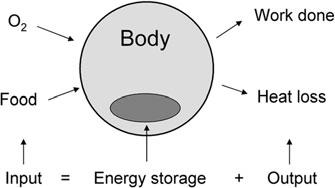
\includegraphics[width=0.6\textwidth]{61.png}
  \caption{Flujo de energía hacia y desde el cuerpo.}
  \label{fig:61}
\end{SCfigure}



Los procesos metabólicos se pueden dividir en reacciones catabólicas y anabólicas. En las reacciones catabólicas, las moléculas complejas se descomponen en otras más simples, con fines tales como el uso de energía. En las reacciones anabólicas, las moléculas simples se combinan para formar otras complejas, con fines tales como el almacenamiento de energía.

El cuerpo utiliza los alimentos para (1) hacer funcionar los órganos, (2) mantener una temperatura constante utilizando parte del calor generado por el funcionamiento de los órganos (mientras que el resto es rechazado), (3) realizar trabajo externo, (4) acumular una reserva de energía almacenada (grasa) para necesidades posteriores, (5) crecer hasta la edad adulta y (6) ayudar al feto a crecer durante el embarazo y luego amamantar a los lactantes. Aproximadamente el $5\text{--}10\%$ de la ingesta de energía de los alimentos se excreta en las heces y la orina.

Primero consideraremos los conceptos básicos de la conservación de la energía (termodinámica). Luego examinaremos el contenido energético de los alimentos y la forma en que se almacenan en el cuerpo. Veremos cuál debe ser la tasa metabólica del cuerpo para realizar tareas. (Esta es técnicamente la tasa catabólica). A continuación, analizaremos cómo el cuerpo pierde energía en forma de calor. Estos pasos están interrelacionados en un modo complejo de retroalimentación y control que se analiza en el Cap. 13.

Para excelentes discusiones generales sobre el metabolismo, véase \cite{10,11,19,20,35,57,89,106}.

\section{Conservación de la energía y flujo de calor}

Repasemos brevemente algunos de los conceptos básicos de la termodinámica y la física del flujo de calor que utilizaremos en esta discusión.

La primera ley de la termodinámica es esencialmente la conservación de la energía en cualquier proceso. Con referencia al cuerpo, se puede expresar como
\begin{equation}
\Delta U = Q - W,
\label{eq:61}
\end{equation}
donde $\Delta U$ es el cambio en la energía almacenada, $Q$ es el flujo de calor hacia el cuerpo y $W$ es el trabajo mecánico realizado por el cuerpo. La energía almacenada disminuye, $\Delta U < 0$, cuando hay flujo de calor desde el cuerpo, $Q < 0$, y trabajo realizado por el cuerpo, $W > 0$. Este tipo de trabajo es de naturaleza puramente mecánica, como al mover y levantar objetos. El flujo de calor incluye la producción de calor a partir del metabolismo ($Q_{\text{met}}$) y la pérdida de calor ($Q_{\text{loss}}$) por radiación, convección, conducción y evaporación. Podemos expresar $Q = Q_{\text{met}} + Q_{\text{loss}}$, donde la producción de calor metabólico es positiva y un $Q_{\text{loss}}$ negativo indica un flujo de calor que se aleja del cuerpo, por lo que
\begin{equation}
\Delta U = Q_{\text{met}} + Q_{\text{loss}} - W.
\label{eq:62}
\end{equation}

$Q_{\text{met}}$ se denomina tasa metabólica (TM).

Las relaciones en termodinámica involucran cantidades de energía que cambian en un proceso en equilibrio y no aquellas que cambian por unidad de tiempo, es decir, la cinética de ese proceso, que involucra las tasas de cambios o flujos de energía. El estudio del metabolismo usualmente involucra tasas y, por lo tanto,
\begin{equation}
\frac{dU}{dt} = \frac{dQ_{\text{met}}}{dt} + \frac{dQ_{\text{loss}}}{dt} - \frac{dW}{dt}
\label{eq:63}
\end{equation}
es más apropiada. (Debemos tener cuidado con los signos. El cuerpo incrementa su energía con términos como $dQ_{\text{met}}/dt$ que son positivos y la pierde con términos como $dQ_{\text{loss}}/dt$ que son negativos. La cantidad de calor que fluye desde el cuerpo es $-dQ_{\text{loss}}/dt$, que es una cantidad positiva).

\begin{table}[htbp]
\centering
\caption{Unidades de potencia}
\label{tab:61}
\begin{tabularx}{0.6\textwidth}{l >{\raggedright\arraybackslash}X}
\toprule
$1\text{ vatio (W)}$ & $= 1\text{ J/s}$ \\
$100\text{ W}$ & $= 1,43\text{ kcal/min}$ \\
$1\text{ caballo de fuerza (hp)}$ & $= 746\text{ W} = 642\text{ kcal/h}$ \\
$1\text{ kcal/min}$ & $= 69,7\text{ W} = 0,094\text{ hp}$ \\
$1\text{ kcal/h}$ & $= 1,162\text{ W}$ \\
\bottomrule
\end{tabularx}
\end{table}

Todos los tipos de energía tienen las mismas unidades, incluyendo el calor (a menudo expresado en términos de calorías) y el trabajo (a menudo expresado en términos de julios). Una conversión importante entre unidades es
\begin{equation}
1\text{ caloría (cal)} = 4,184\text{ julios (J)}.
\label{eq:64}
\end{equation}

Una kilocaloría ($1\text{ kcal} = 1000\text{ cal}$) a veces se llama $1\text{ Cal}$, la cual también se conoce como caloría alimentaria. El contenido energético de los alimentos siempre se expresa en términos de estas unidades de $\text{Cal}$ ($\text{kcal}$). Las relaciones entre las diversas unidades de potencia (energía/tiempo) se presentan en la Tabla 6.1.

Un concepto importante en la física térmica del cuerpo es la capacidad calorífica $C$, que es la energía (or más específicamente, el calor) requerida para elevar la temperatura $T$ de un objeto en $1^\circ\text{C}$. La capacidad calorífica por unidad de volumen o masa es el calor específico $c$. La capacidad calorífica es una propiedad extensiva de un objeto dado, mientras que el calor específico es una propiedad intensiva de un material. (Esta clasificación es análoga a la de las propiedades mecánicas descritas en el Cap. 4). Si el calor específico se expresa por unidad de masa, se puede convertir a calor específico por unidad de volumen multiplicándolo por la densidad de masa $\rho$. La capacidad calorífica $C$ es el calor específico (expresado por unidad de masa) $\times$ la masa total del objeto $m$, por lo que $C = mc$.

El aumento de temperatura $\Delta T$ de un objeto con un flujo de calor $Q$ hacia el cuerpo es
\begin{equation}
\Delta T = \frac{Q}{mc}.
\label{eq:65}
\end{equation}

Para el agua, $c_{\text{water}} = 1{,}0\text{ cal/g-}^\circ\text{C} = 1{,}0\text{ kcal/kg-}^\circ\text{C}$. Aunque el cuerpo humano contiene mucha agua, el calor específico promedio del cuerpo es un poco menor, $c_{\text{b}} = 0{,}83\text{ cal/g-}^\circ\text{C}$ (equivalente a $0{,}83\text{ kcal/kg-}^\circ\text{C}$). Esto significa que se necesitan $83\text{ kcal}$ para elevar la temperatura de una persona de $100\text{ kg}$ en $1^\circ\text{C}$. Estas $83\text{ kcal}$ ($83\text{ calorías alimentarias}$) representan aproximadamente el contenido de energía alimentaria de una rebanada de pan. Surge una pregunta obvia: si la mayor parte de nuestra energía metabolizada se convierte en calor, ¿por qué la temperatura de nuestro cuerpo no aumenta en $1,0^\circ\text{C} = 1,8^\circ\text{F}$ cada vez que comemos y metabolizamos una rebanada de pan? Somos muy afortunados de que no sea así. (La razón es la pérdida de calor por parte del cuerpo).

La capacidad calorífica de un objeto describe cómo cambia su temperatura con el tiempo debido al flujo de calor hacia y desde el objeto. La conductividad térmica $K$ describe cómo varía la temperatura ($\Delta T$) espacialmente debido al flujo de calor entre diferentes regiones que están separadas por una distancia $\Delta x$. (A la inversa, también describe cuánto calor fluye debido a esta variación espacial de la temperatura). Esta relación es
\begin{equation}
\frac{1}{A} \frac{dQ}{dt} = -K \frac{dT}{dx} \sim -K \frac{\Delta T}{\Delta x}.
\label{eq:66}
\end{equation}

El lado izquierdo es la cantidad de calor que fluye por unidad de área $A$ por unidad de tiempo, y también se denomina flujo de calor. El signo menos indica que el calor fluye de las regiones más calientes a las más frías. Cuando existe una distancia bien definida $d = \Delta x$ entre dos regiones de temperatura diferente pero uniforme, por ejemplo debido al grosor de la ropa o a una capa límite de aire, podemos definir un coeficiente de transferencia de calor por unidad de área $h = K/d$ y entonces
\begin{equation}
\frac{1}{A} \frac{dQ}{dt} = -h \Delta T.
\label{eq:67}
\end{equation}

El flujo de calor debido a otros mecanismos, como la radiación, a menudo se puede expresar en términos de las ecuaciones (\ref{eq:66}) o (\ref{eq:67}).

Una consecuencia de la termodinámica es que las máquinas que convierten la energía química en calor y utilizan ese calor para realizar trabajo mecánico, llamadas máquinas térmicas, tienen una eficiencia limitada para realizar dicho trabajo mecánico útil. Una máquina térmica ideal tiene una eficiencia máxima de $\epsilon = 1 - (T_{\text{c}}/T_{\text{h}})$ cuando funciona a una temperatura $T_{\text{h}}$ y rechaza calor a una temperatura más baja $T_{\text{c}}$ (ambas expresadas en $\text{K}$). Los seres humanos funcionan internamente a aproximadamente $T_{\text{h}} = 310\text{ K}$ y rechazan calor a un ambiente a $T_{\text{c}} \simeq 293\text{ K}$, por lo que $\epsilon$ sería del $5,5\%$ si fuéramos máquinas térmicas. Esto es mucho menor que la eficiencia de aproximadamente el $25\%$ de los seres humanos al convertir la energía química en trabajo mecánico. Esto no es una contradicción porque utilizamos la energía química directamente para realizar trabajo mecánico, como se vio en el Cap. 5, y no producimos calor en un paso intermedio.

\section{Contenido de energía del combustible corporal}

Existe cierta similitud entre la oxidación metabólica y la combustión, a pesar de que el cuerpo no «quema» sus combustibles en oxígeno. Es útil aprender sobre la combustión de estos combustibles porque la combustión indica la cantidad máxima de energía disponible a partir de la ruptura y el reordenamiento de los enlaces. La oxidación metabólica es un poco menos eficiente, como veremos. Las energías de combustión (entalpías) se obtienen a partir de la calorimetría de «bomba», en la cual los materiales se queman en recipientes de paredes gruesas. Las energías resultantes son útiles y aproximadamente correctas, aunque las condiciones de esta bomba —su funcionamiento a volumen constante y la temperatura real de la «bomba»— son diferentes a las del cuerpo. Por ejemplo, muchos procesos en el cuerpo ocurren a presión constante y no a volumen constante.

\textbf{Glucosa.} El metabolismo de la glucosa es representativo del de los carbohidratos. Si comenzamos con $1\text{ mol}$ de glucosa ($180\text{ g}$, $6,02 \times 10^{23}$ moléculas) y la oxidamos con $6\text{ mol}$ de moléculas de oxígeno ($192\text{ g} = 134,4\text{ L}$ en condiciones estándar, dado que hay $22,4\text{ L/mol}$ a $1\text{ atm}$ y $0^\circ\text{C}$), se producen $6\text{ mol}$ de dióxido de carbono, $6\text{ mol}$ de agua ($108\text{ g}$, $108\text{ mL}$) y $686\text{ kcal}$ de energía. Esto se puede representar mediante
\begin{equation}
\text{C}_6\text{H}_{12}\text{O}_6 + 6\text{O}_2 \rightarrow 6\text{CO}_2 + 6\text{H}_2\text{O} + 686\text{ kcal}.
\label{eq:68}
\end{equation}

La energía producida por masa de combustible es $686\text{ kcal}/180\text{ g} = 3,80\text{ kcal/g}$ de glucosa. También definimos un equivalente calórico, la energía producida por litro de oxígeno consumido, que aquí es $686\text{ kcal}/134,4\text{ L de O}_2 = 5,5\text{ kcal/L de O}_2$.

En la oxidación metabólica el cuerpo combina este $1\text{ mol}$ de glucosa con $30\text{--}32\text{ mol}$ de ADP y $30\text{--}32\text{ mol}$ del grupo fosfato $\text{P}_i$ para formar $30\text{--}32\text{ mol}$ de la molécula de almacenamiento de energía ATP.

\textbf{Ácido palmítico.} La oxidación del ácido palmítico es representativa de la de los ácidos grasos. La oxidación procede mediante
\begin{equation}
\text{CH}_3(\text{CH}_2)_{14}\text{COOH} + 23\text{O}_2 \rightarrow 16\text{CO}_2 + 16\text{H}_2\text{O} + 2397\text{ kcal},
\label{eq:69}
\end{equation}
de modo que $1\text{ mol}$ ($256,4\text{ g}$) de ácido palmítico es quemado por $23\text{ mol}$ ($515,2\text{ L}$) de oxígeno para formar $16\text{ mol}$ ($358,4\text{ L}$) de cada uno de dióxido de carbono y agua, y $2397\text{ kcal}$. La energía liberada es $2397\text{ kcal}/256,4\text{ g} = 9,3\text{ kcal/g}$ y el equivalente calórico es $2397\text{ kcal}/515,2\text{ L de O}_2 = 4,7\text{ kcal/L de O}_2$. En la oxidación metabólica, el cuerpo utiliza este $1\text{ mol}$ de ácido palmítico para combinar $106\text{ mol}$ de ADP y del grupo fosfato $\text{P}_i$ para formar $106\text{ mol}$ de ATP.

Al comparar la glucosa $\text{C}_6\text{H}_{12}\text{O}_6$ con el ácido palmítico $\text{C}_{16}\text{H}_{32}\text{O}_2$, ambos tienen la misma relación $1:2$ de $\text{C}$ e $\text{H}$, por lo que, después de la oxidación, se forman números iguales de moles de $\text{CO}_2$ y $\text{H}_2\text{O}$ en ambos casos. Sin embargo, el ácido palmítico y otras grasas tienen mucho menos oxígeno por $\text{C}$ e $\text{H}$ que la glucosa y otros carbohidratos, por lo que se consume una menor masa de ellos por mol de $\text{CO}_2$ y $\text{H}_2\text{O}$ formado. (La masa molar del ácido palmítico es de $256\text{ g}$, y esto es mucho menor que la masa molar de $480\text{ g}$ del «carbohidrato equivalente» $\text{C}_{16}\text{H}_{32}\text{O}_{16}$). Alternativamente (y de manera equivalente), podemos decir que las grasas están menos oxidadas, están más reducidas y tienen un mayor poder reductor que los carbohidratos.

Los calores de combustión de los carbohidratos, las grasas y las proteínas difieren ligeramente para diferentes tipos de alimentos. Para los carbohidratos, varían de $3,7$ a $4,4\text{ kcal/g}$ y se pueden promediar y agrupar en diferentes grupos de alimentos con $3,90$, $3,95$, $4,00$ y $4,20\text{ kcal/g}$ respectivamente para productos de origen animal, carnes y productos lácteos; azúcares; frutas; cereales, legumbres, almidones y verduras. Los calores de combustión por gramo para grasas y aceites varían de $\sim 9,0\text{--}9,5\text{ kcal/g}$, y estos se agrupan en $9,25$, $9,30$ y $9,50\text{ kcal/g}$ respectivamente para productos lácteos; cereales, verduras y frutas; y carne, pescado y huevos. La comparación es más compleja para los componentes alimenticios nitrogenados, que generalmente se denominan proteínas en este campo. Esto incluye todos los compuestos que contienen nitrógeno y generalmente se determina a partir de la masa analizada de nitrógeno en los alimentos. Para las proteínas verdaderas, a veces llamadas proteidos en este campo, hay $6,25\text{ g}$ de proteidos por gramo de $\text{N}$ ($16\%$ de $\text{N}$), que tienen calores de combustión de $\sim 5,8\text{ kcal/g de proteína}$. Para otros componentes nitrogenados de los alimentos, a veces llamados no proteidos, la fracción de $\text{N}$ y los calores de combustión son diferentes. Por ejemplo, para la gelatina, la creatina (común en alimentos de origen animal) y la asparagina (alimentos de origen vegetal), los calores de combustión son respectivamente $5,27$, $4,27$ y $3,45\text{ kcal/g}$, lo cual es inferior al de los proteidos. El promedio ponderado (utilizando los métodos abordados en el Problema 6.26) conduce a calores de combustión promedio de $5,00$, $5,20$, $5,65$, $5,70$, $5,75$ y $5,80\text{ kcal/g}$ respectivamente para las proteínas (generales) en las verduras (que son $60\%$ proteidos); frutas ($70\%$ proteidos); productos lácteos y carne; legumbres ($96\%$ proteidos); huevos; y cereales ($96\%$ proteidos) \cite{68}. El calor de combustión para el alcohol es de $7,07\text{ kcal/g}$. El etanol tiene un alto calor de combustión y, como veremos, proporciona una gran cantidad de aporte calórico, lo que explica por qué es fácil ganar peso al beber alcohol, como la cerveza. Si tu aporte calórico proviene principalmente del alcohol, puedes «morir de hambre» en el sentido de que tus necesidades calóricas están cubiertas, pero no tus necesidades de micronutrientes, como vitaminas y minerales. (Ten en cuenta que algunos de los valores promedio que se presentan aquí obtenidos de \cite{68} difieren ligeramente de los enumerados en la Tabla 6.2 obtenidos de \cite{35}).

Estas energías liberadas por unidad de masa, o calores de combustión, son las energías máximas disponibles, y en realidad se denominan energías de calorimetría de bomba porque a menudo se miden en explosiones controladas en laboratorio. La cantidad disponible para el cuerpo es algo menor y se define como el valor calórico. La Tabla 6.2 muestra los valores calóricos promedio y los equivalentes calóricos de los tipos de combustibles corporales básicos.

\begin{table}[htbp]
\centering
\caption{Contenido calórico promedio de los alimentos}
\label{tab:62}
\footnotesize
\begin{tabularx}{\textwidth}{>{\hsize=0.8\hsize\raggedright\arraybackslash}X >{\hsize=0.9\hsize\centering\arraybackslash}X >{\hsize=1.1\hsize\centering\arraybackslash}X >{\hsize=1.1\hsize\centering\arraybackslash}X >{\hsize=1.1\hsize\centering\arraybackslash}X >{\hsize=1.0\hsize\centering\arraybackslash}X}
\toprule
\textbf{Alimento} & \textbf{Valor calórico} & \textbf{Energía de} & \textbf{Equivalente} & \textbf{Producción de} & \textbf{RER} \\
 & \textbf{neto (kcal/g)} & \textbf{calorimetría (kcal/g)} & \textbf{calórico ($\text{kcal/L O}_2$)} & \textbf{CO$_2$ ($\text{kcal/L CO}_2$)} & \textbf{($\text{L CO}_2/\text{L O}_2$)} \\
\midrule
Carbohidrato & 4,02 & 4,10 & 5,05 & 5,05 & 1,0 \\
Proteína & 4,20 & 5,65 & 4,46 & 5,57 & 0,80 \\
Etanol & 7,00 & 7,10 & 4,86 & 7,25 & 0,67 \\
Grasa & 8,98 & 9,45 & 4,74 & 6,67 & 0,71 \\
\bottomrule
\end{tabularx}
\begin{flushleft}
    \small RER es la relación de intercambio respiratorio.\\
    Utilizando datos de \cite{35}.
\end{flushleft}
\end{table}

Los valores calóricos son inferiores a los de la calorimetría de bomba debido a las pérdidas durante la digestión, que promedian el $2\%$ para los carbohidratos, el $5\%$ para las grasas y el $8\%$ para las proteínas, más una pérdida adicional del $17\%$ de la energía de las proteínas en la orina \cite{68}. Las pequeñas pérdidas para el etanol, de $\sim 2\%$, se encuentran en la orina y en el aire espirado. Con estas correcciones y otras relacionadas, el valor calórico promedio de los carbohidratos y las proteínas es $\simeq 4\text{ kcal/g}$ y el de las grasas es $\simeq 9\text{ kcal/g}$, los cuales se conocen como los valores del sistema de Atwater \cite{68}. (Cada $\text{kcal}$ es una caloría alimentaria, o $\text{Cal}$, que se denomina caloría en las etiquetas de los envases de alimentos).

El uso de estos valores suele ser una aproximación muy buena, pero no es perfecto. Los valores de la energía digerible a partir de estas fuentes para alimentos específicos se presentan en \cite{100}, junto con el contenido de nutrientes del alimento. Una discusión más general sobre el contenido de energía y nutrientes se encuentra en \cite{23}, y un análisis más detallado sobre el contenido de energía se presenta en \cite{6,68}. Estos valores calóricos se pueden comparar con los combustibles comunes de calefacción y automoción: gasolina, $11,4\text{ kcal/g}$; carbón, $8,0\text{ kcal/g}$; y madera de pino, $18,5\text{ kcal/g}$. Las densidades de almacenamiento de energía de diferentes combustibles químicos se comparan en la Tabla 6.3.

Podemos poner el valor calórico en perspectiva desarrollando una unidad estándar: El Donut. Utilizaremos $1$ Donut Entenmann's\texttrademark\ Rich Frosted (es decir, glaseado de chocolate) como el donut estándar. La etiqueta del envase indica que un donut contiene $18\text{ g}$ de grasa, $29\text{ g}$ de carbohidratos y $2\text{ g}$ de proteína (en 2005), por lo que podemos estimar el valor calórico de cada donut, como se muestra en la Tabla 6.4. Vemos que $49\text{ g}$ de la masa total de $57\text{ g}$ del donut tienen contenido calórico. Nuestro cálculo sugiere que hay $286\text{ kcal}$ ($286\text{ calorías alimentarias}$) por donut. El envase dice que hay $280\text{ kcal}$ por donut, lo cual tomaremos como el contenido calórico del donut estándar. Estos valores son muy consistentes entre sí porque hemos utilizado valores calóricos promedio para la grasa, los carbohidratos y la proteína. Además, hemos redondeado los valores calóricos y ellos han proporcionado los valores de la masa de cada combustible corporal en gramos redondeados al entero más cercano (según lo requerido por la FDA de los EE.~UU. (Administración de Alimentos y Medicamentos)). (Para más información sobre el redondeo, véanse los Problemas 6.11 y 6.12). Aproximadamente el $57\%$ de las calorías ($162\text{ kcal}/286\text{ kcal}$) proviene de la grasa. Pronto determinaremos cuánto esfuerzo físico se necesita para eliminar las consecuencias «engordantes» de comer un donut estándar. Además, notamos que durante la redacción de esta segunda edición (2015), el Donut Entenmann's\texttrademark\ Rich Frosted tenía $300\text{ kcal}$. Exploraremos este aspecto de nuestro mundo en constante cambio en el Problema 6.15. En cualquier caso, seguiremos asumiendo que el donut estándar tiene $280\text{ kcal}$. (Los Problemas 6.13 y 6.14 abordan otros posibles donuts estándar).

\begin{table}[htbp]
\centering
\caption{Densidad de almacenamiento de energía para combustibles químicos}
\label{tab:63}
\small
\begin{tabularx}{\textwidth}{Xcc}
\toprule
\textbf{Combustible de almacenamiento de energía} & \textbf{Densidad de almacenamiento ($\text{J/m}^3$)} & \textbf{Densidad de almacenamiento ($\text{J/kg}$)} \\
\midrule
ATP & $1,4 \times 10^8$ & $1,0 \times 10^5$ \\
Gas H$_2$, $10^3\text{ atm}$ & $4,9 \times 10^9$ & $1,2 \times 10^8$ \\
Nitroglicerina & $1,0 \times 10^{10}$ & $6,3 \times 10^6$ \\
Glicina (aminoácido) & $1,0 \times 10^{10}$ & $6,5 \times 10^6$ \\
Madera & $1,1 \times 10^{10}$ & $1,9 \times 10^7$ \\
Urea & $1,4 \times 10^{10}$ & $1,1 \times 10^7$ \\
Metanol & $1,8 \times 10^{10}$ & $2,2 \times 10^7$ \\
Proteína vegetal & $2,3 \times 10^{10}$ & $1,7 \times 10^7$ \\
Acetona & $2,4 \times 10^{10}$ & $3,1 \times 10^7$ \\
Glucosa & $2,4 \times 10^{10}$ & $1,6 \times 10^7$ \\
Glucógeno (almidón) & $2,5 \times 10^{10}$ & $1,8 \times 10^7$ \\
Proteína animal & $2,5 \times 10^{10}$ & $1,8 \times 10^7$ \\
Carbohidrato & $2,6 \times 10^{10}$ & $1,7 \times 10^7$ \\
Gasolina & $2,8 \times 10^{10}$ & $4,4 \times 10^7$ \\
Butano & $3,0 \times 10^{10}$ & $4,9 \times 10^7$ \\
Grasa & $3,3 \times 10^{10}$ & $3,9 \times 10^7$ \\
Colesterol (lípido) & $4,2 \times 10^{10}$ & $3,9 \times 10^7$ \\
H$_2$ sólido ($10^5\text{ atm}$) & $7,2 \times 10^{10}$ & $1,2 \times 10^8$ \\
Diamante & $1,2 \times 10^{11}$ & $3,3 \times 10^7$ \\
\bottomrule
\end{tabularx}
\begin{flushleft}
    \small Nota: tenga en cuenta que $10^{10}\text{ J/m}^3 = 2,39\text{ kcal/cm}^3$ y $10^7\text{ J/kg} = 2,39\text{ kcal/g}$.\\
    Utilizando datos de \cite{38}.
\end{flushleft}
\end{table}

\begin{table}[htbp]
\centering
\caption{Valor calórico de 1 donut Entenmann's\texttrademark\ Rich Frosted (en 2005)}
\label{tab:64}
\begin{tabularx}{0.6\textwidth}{X}
\toprule
$18\text{ g de grasa} \times 9\text{ kcal/g} = 162\text{ kcal}$ \\
$29\text{ g de carbohidratos} \times 4\text{ kcal/g} = 116\text{ kcal}$ \\
$2\text{ g de proteína} \times 4\text{ kcal/g} = 8\text{ kcal}$ \\
\midrule
$49\text{ g en total} = 286\text{ kcal}$ \\
\bottomrule
\end{tabularx}
\end{table}

La energía liberada por litro de $\text{O}_2$ (equivalente calórico) es bastante constante para todos los combustibles corporales, variando de $\sim 4,5$ a $5,5\text{ kcal/L de O}_2$. Para una «dieta mixta», el equivalente calórico se estima en $4,83\text{ kcal/L de O}_2$ y la producción de $\text{CO}_2$ en $5,89\text{ kcal/L de CO}_2$.

La relación de intercambio respiratorio (RER) (o cociente respiratorio (RQ)) es otra forma de caracterizar los procesos metabólicos. Es el número de moles de $\text{CO}_2$ producidos dividido por el número de moles de $\text{O}_2$ utilizados, y es una medida de cuánto dióxido de carbono necesita ser liberado en la respiración en relación con la cantidad de oxígeno que el cuerpo necesita incorporar mediante la respiración. Vemos que $\text{RER} = 6\text{ L de CO}_2/6\text{ L de O}_2 = 1,0$ para la oxidación de la glucosa y $16\text{ L}/23\text{ L} = 0,7$ para la oxidación del ácido palmítico. Normalmente es de $0,8$ para la oxidación de proteínas.

\subsection{Energía metabolizable}

Deberíamos tener un poco más de cuidado al definir qué cantidad de la energía de los alimentos se metaboliza y se utiliza realmente, aunque estas distinciones relativamente sutiles en la energética corporal puedan no ser de gran importancia para nosotros aquí. La tasa de energía aparentemente digerida es la diferencia entre la tasa de ingesta de energía de la dieta y la tasa de pérdida de energía en las heces. La tasa de obtención de energía metabolizable ($\text{ME}$), $d(\text{ME})/dt$, es la diferencia entre la tasa de ingesta de energía de la dieta y la suma de las tasas de pérdida de energía en las heces, la orina y los gases combustibles. Esta es la tasa real a la que la energía se pone a disposición del cuerpo \cite{11}.

La Tabla 6.5 muestra el contenido calórico y los componentes de varios tipos de alimentos. El contenido calórico por unidad de masa depende de las cantidades relativas de carbohidratos, proteínas y grasas, y de etanol para las bebidas alcohólicas, así como de las cantidades de agua y «ceniza». Para comparar, nuestro donut estándar tiene $280\text{ kcal}$, o $280\text{ kcal}/57\text{ g} = 4,91\text{ kcal/g}$.

\begin{table}[htbp]
\centering
\caption{Componentes y energía (kcal) de partes comestibles de alimentos comunes}
\label{tab:65}
\small
\begin{tabularx}{\textwidth}{Xcccccc}
\toprule
\textbf{Alimento, tamaño de la porción} & \textbf{Masa (g)} & \textbf{Energía (kcal)} & \textbf{Carb.$^{\text{a}}$ (g)} & \textbf{Proteína (g)} & \textbf{Grasa (g)} & \textbf{Agua (\%)} \\
\midrule
\multicolumn{7}{l}{\textit{Granos y pasteles}} \\
Pan, blanco, 1 rebanada & 25 & 67 & 12 & 2 & 1 & 37 \\
Avena, regular, 1 taza preparada & 234 & 145 & 25 & 6 & 2 & 85 \\
Pastel amarillo, glaseado de chocolate, 1 pieza & 64 & 243 & 35 & 2 & 11 & 22 \\
Pastel de queso, 1/6 de pastel de 17 oz & 80 & 257 & 20 & 4 & 18 & 46 \\
\midrule
\multicolumn{7}{l}{\textit{Lácteos}} \\
Leche, entera, 1 taza & 244 & 150 & 11 & 8 & 8 & 88 \\
Mantequilla, con sal, barra de 1/4 lb & 113 & 813 & $\text{Tr}^{\text{b}}$ & 1 & 92 & 16 \\
Queso cheddar, 1 oz & 28 & 114 & $\text{Tr}$ & 7 & 9 & 37 \\
Queso cottage, $4\%$, 1 taza & 225 & 233 & 6 & 28 & 10 & 79 \\
Helado, chocolate, 1/2 taza & 66 & 143 & 19 & 3 & 7 & 56 \\
Huevos, crudos, 1 grande & 50 & 75 & 1 & 6 & 5 & 75 \\
\midrule
\multicolumn{7}{l}{\textit{Carne y pescado}} \\
Pollo, solo carne, asado, 1/2 pechuga & 86 & 142 & 0 & 27 & 3 & 65 \\
Carne de res, molida, $79\%$ magra, a la parrilla, 3 oz & 85 & 231 & 0 & 21 & 16 & 56 \\
Salmón, a la parrilla, 3 oz & 85 & 184 & 0 & 23 & 9 & 62 \\
\bottomrule
\end{tabularx}
\begin{flushleft}
    $^{\text{a}}$ Carbohidratos.\\
    $^{\text{b}}$ Traza (cantidad insignificante).\\
    Utilizando datos de \cite{41}.
\end{flushleft}
\end{table}

\begin{table}[htbp]
\centering
\addtocounter{table}{-1}
\caption{Componentes y energía (kcal) de partes comestibles de alimentos comunes (continuación)}
\small
\begin{tabularx}{\textwidth}{Xcccccc}
\toprule
\textbf{Alimento, tamaño de la porción} & \textbf{Masa (g)} & \textbf{Energía (kcal)} & \textbf{Carb.$^{\text{a}}$ (g)} & \textbf{Proteína (g)} & \textbf{Grasa (g)} & \textbf{Agua (\%)} \\
\midrule
\multicolumn{7}{l}{\textit{Frutas, verduras, frutos secos y aceites}} \\
Manzana, cruda, sin pelar, 1 entera & 138 & 81 & 21 & $\text{Tr}$ & $\text{Tr}$ & 84 \\
Albaricoques, crudos, sin hueso, 1 entero & 35 & 17 & 4 & $\text{Tr}$ & $\text{Tr}$ & 86 \\
Albaricoques, secos, sulfurados, 10 mitades & 35 & 83 & 22 & 1 & $\text{Tr}$ & 31 \\
Naranja, pelada, 1 entera & 131 & 62 & 15 & 1 & $\text{Tr}$ & 87 \\
Zanahorias, crudas, $7\ \frac{1}{2}\text{ in}$ de largo & 72 & 31 & 7 & 1 & $\text{Tr}$ & 88 \\
Patata, horneada, con piel & 202 & 220 & 51 & 5 & $\text{Tr}$ & 71 \\
Patatas fritas, porción mediana & 134 & 458 & 53 & 6 & 25 & 35 \\
Maníes, tostados en seco, 1 taza & 146 & 854 & 31 & 35 & 73 & 2 \\
Nueces, 1 taza picada & 120 & 785 & 16 & 18 & 78 & 4 \\
Aceite de canola, 1 taza & 218 & 1927 & 0 & 0 & 218 & 0 \\
\midrule
\multicolumn{7}{l}{\textit{Bebidas}} \\
Refresco de cola, $12\text{ fl oz}$ & 370 & 152 & 38 & 0 & 0 & 89 \\
Cerveza (regular), $12\text{ fl oz}$ & 355 & 146 & 13 & 1 & 0 & 92 \\
Ginebra, vodka, whisky, grado 86, $1,5\text{ fl oz}$ & 42 & 105 & $\text{Tr}$ & 0 & 0 & 64 \\
Vino, tinto, $3,5\text{ fl oz}$ & 103 & 74 & 2 & $\text{Tr}$ & 0 & 89 \\
\bottomrule
\end{tabularx}
\begin{flushleft}
    $^{\text{a}}$ Carbohidratos.\\
    $^{\text{b}}$ Traza (cantidad insignificante).\\
    Utilizando datos de \cite{41}.
\end{flushleft}
\end{table}

La Tabla 6.6 muestra la entalpía de combustión para diferentes tipos de leche; esto constituye energía consumida y no necesariamente metabolizable. La entalpía disponible a partir de grasa, proteína y carbohidratos es bastante diferente para cada fuente. Con una dieta de $42\%$ de grasa y $18\%$ de proteína, aproximadamente el $89,3\%$ de los alimentos consumidos suele ser metabolizable, lo que significa que esta es la fracción del contenido energético de los alimentos que representa energía metabolizable. Aproximadamente el $5,8\%$ de la energía consumida se pierde en las heces, el $4,5\%$ en la orina y el $0,4\%$ se pierde en forma de metano. La diferencia entre el contenido energético utilizando los factores de Atwater y la energía consumible puede ser mucho mayor que esta en algunos alimentos. Por ejemplo, es de $\sim 30\%$ para las almendras \cite{76}.

\begin{table}[htbp]
\centering
\caption{Contenido alimentario de la leche}
\label{tab:66}
\begin{tabularx}{\textwidth}{Xccccc}
\toprule
\textbf{Especie} & \textbf{Entalpía de} & \multicolumn{3}{c}{\textbf{Distribución de la entalpía (\%)}} & \textbf{Materia} \\
\cmidrule(lr){3-5}
 & \textbf{combustión (kcal/g)} & \textbf{Grasa} & \textbf{Proteína} & \textbf{Carbohidrato} & \textbf{seca (\%)} \\
\midrule
Humana & 0,69 & 54 & 7 & 39 & 12,4 \\
Vaca & 0,71 & 48 & 26 & 26 & 12,4 \\
Cabra & 0,69 & 50 & 22 & 27 & 12,0 \\
Caballo & 0,51 & 23 & 22 & 54 & 10,5 \\
Foca (peletera del norte) & 5,09 & 88 & 11 & 0,1 & 61,0 \\
\bottomrule
\end{tabularx}
\begin{flushleft}
    \small Utilizando datos de \cite{11}.
\end{flushleft}
\end{table}

Dedicamos relativamente poco tiempo y energía a metabolizar los alimentos debido a su alto valor calórico y digestibilidad (y por lo tanto tenemos mucho tiempo para participar en actividades distintas a comer y digerir alimentos). A menudo afectamos ambos mediante el procesamiento de alimentos, por lo que el verdadero valor calórico o $\text{ME}$ de un alimento depende no solo de su calor de combustión y de las pérdidas metabólicas descritas anteriormente, sino de cómo lo procesemos antes de consumirlo \cite{100}. El procesamiento de los alimentos al cocinarlos aumenta nuestra ingesta calórica y de nutrientes después de comerlos en comparación con los alimentos que se comen crudos \cite{14,21,56}. En algunos casos, la ingesta calórica se puede incrementar en comparación con los alimentos crudos mediante procesamiento mecánico, como machacar, moler o cortar los alimentos en trozos pequeños. El costo energético de metabolizar los alimentos disminuye en $\sim 10\%$ cuando se procesan en trozos componentes más pequeños (como el procesamiento de maníes para obtener mantequilla de maní) \cite{14,56}. La cocción de tubérculos (estructuras de plantas que se expanden para almacenar energía, como las patatas (tubérculos de tallo) y las patatas dulces y ñames (tubérculos de raíz)) convierte los almidones de estructuras semicristalinas a materiales amorfos que se hidrolizan fácilmente a azúcares. La cocción de la carne aumenta la ingesta calórica porque desnaturaliza las proteínas, haciéndolas más digeribles, y facilita la separación de las fibras musculares, aumentando el área expuesta para las actividades digestivas. De manera similar, la digestibilidad de los huevos cocidos ($\sim 93\%$) supera a la de los huevos crudos ($\sim 58\%$) \cite{31,32}. La cocción también reduce la energía necesaria para combatir enfermedades que podrían ser causadas por comer algunos alimentos crudos. La forma en que el procesamiento de alimentos afecta sus propiedades mecánicas se describe en el Cap. 4.

El tiempo promedio de retención de los alimentos en el tracto digestivo humano es de $46\text{ h}$; la primera aparición de los residuos de los alimentos ocurre en aproximadamente un tercio de este tiempo medio y la última en aproximadamente cuatro veces este tiempo.

De manera muy aproximada, se necesitan $10\text{ kcal}$ de energía para producir, enviar y procesar cada $1\text{ kcal}$ de energía alimentaria (y esta cantidad es muy diferente para los distintos tipos de alimentos) \cite{56,80}.

\subsection{Almacenamiento de energía}

La energía puede ser retenida o secretada (como leche) por el cuerpo como la entalpía de los tejidos $R$ (que incluye grasa, proteína y carbohidratos). (La entalpía (o contenido de calor) es la energía térmica máxima que se puede obtener a presión constante). La tasa a la que se retiene la entalpía, $dR/dt$, es la diferencia entre la tasa de entrada de energía metabolizable y la producción de calor a través del metabolismo
\begin{equation}
\frac{dR}{dt} = \frac{d(\text{ME})}{dt} - \frac{dQ_{\text{met}}}{dt}.
\label{eq:610}
\end{equation}
(Esto ignora la lactancia). Combinamos esto con la ecuación (6.3) para obtener
\begin{equation}
\frac{dR}{dt} = \frac{d(\text{ME})}{dt} + \frac{dQ_{\text{loss}}}{dt} - \frac{dW}{dt} - \frac{dU}{dt}.
\label{eq:611}
\end{equation}

Cuando no se consumen alimentos ($d(\text{ME})/dt = 0$), $dR/dt$ es negativo y su magnitud es el calor de catabolismo de los tejidos corporales. A medida que se consumen más alimentos, $dR/dt$ aumenta, se utiliza menos energía almacenada (o retenida) y se incrementa la producción de calor; este aumento en la producción de calor es el efecto dinámico específico o efecto termogénico de los alimentos. Cuando la retención de energía es cero durante varios días (de modo que no se utiliza ni se forma energía almacenada neta y el promedio de $dR/dt$ es cero), la energía dietética de entrada $\text{ME}$ es la requerida para el mantenimiento. Para valores mayores de $\text{ME}$, la energía se almacena en el cuerpo.

La Tabla 6.7 muestra los resultados de experimentos calorimétricos para personas que están en ayunas (para quienes la energía almacenada en proteínas y grasas se convierte en calor), que comen y no hacen ejercicio (quienes tienen un almacenamiento neto de grasa corporal) y que comen y hacen ejercicio (para quienes una pequeña cantidad de energía almacenada se convierte en calor, a pesar de que hay una mayor ingesta de alimentos).

\begin{figure}[htbp]
  \centering
  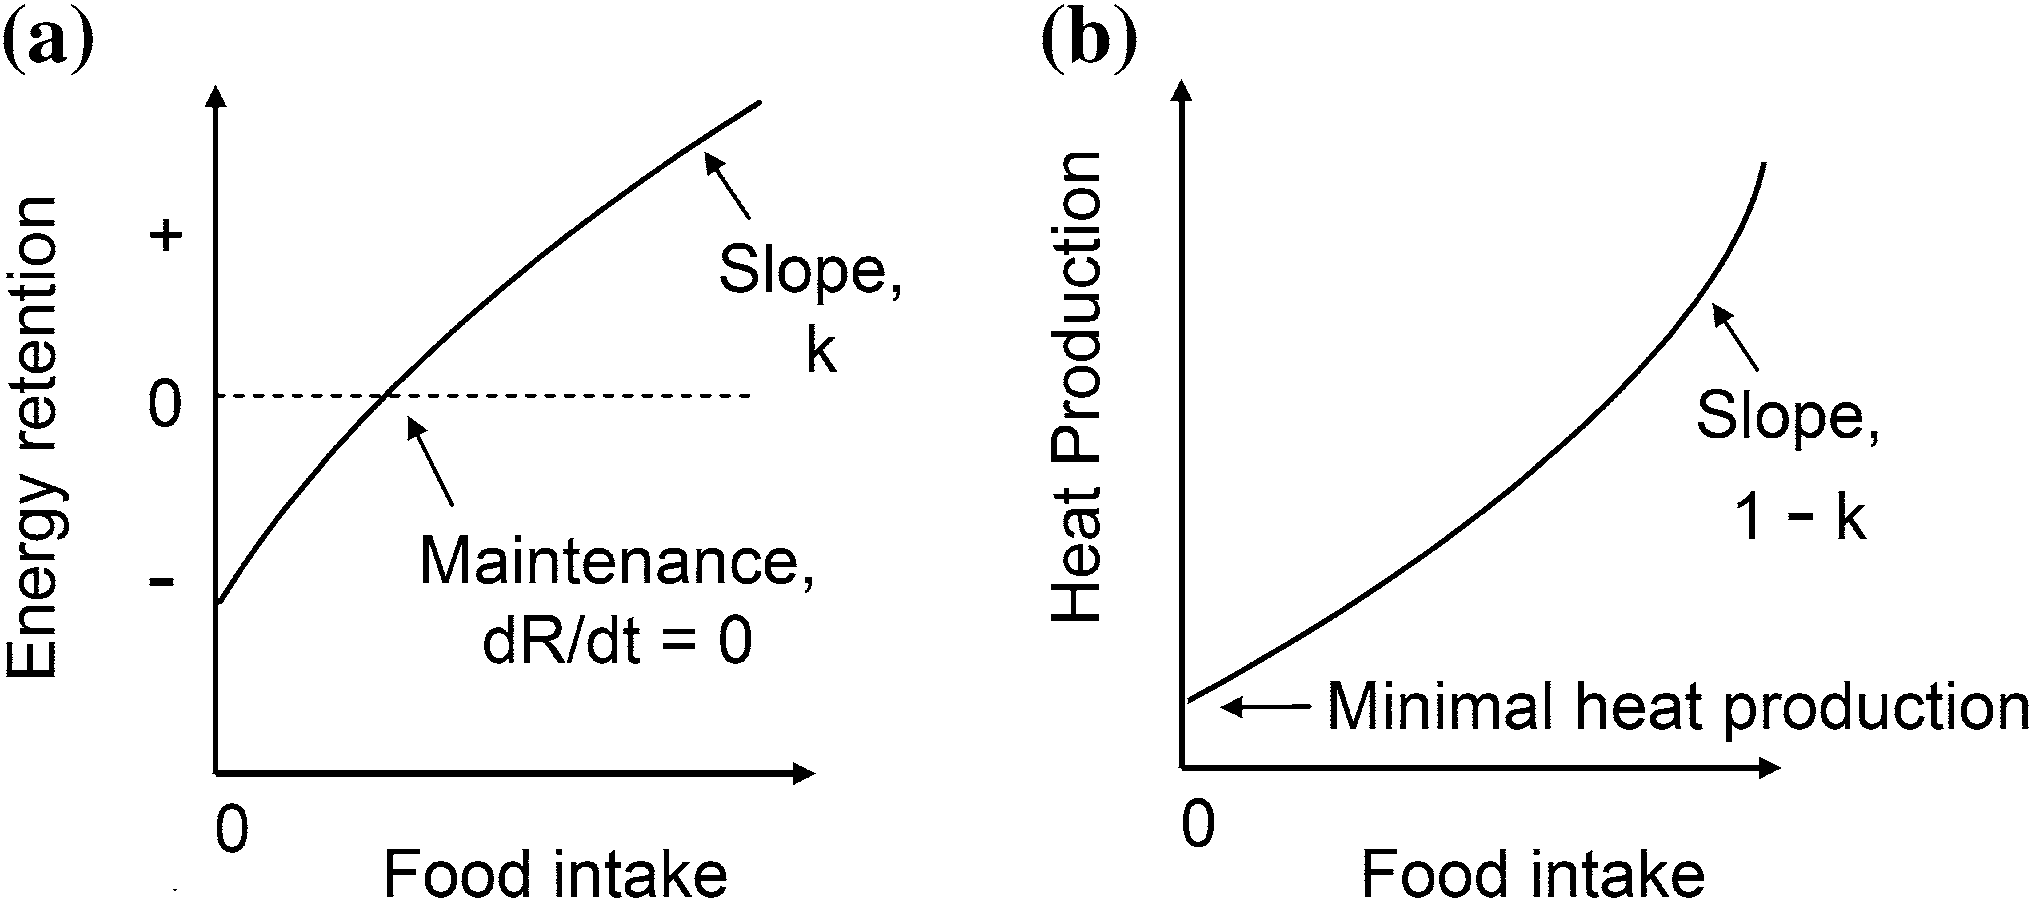
\includegraphics[width=0.8\textwidth]{62.png}
  \caption{Retención de energía y producción de calor en el cuerpo frente a la ingesta de alimentos (basado en \cite{11}).}
  \label{fig:62}
\end{figure}



\begin{table}[htbp]
\centering
\caption{Experimentos calorimétricos, cada uno promediado sobre varias ejecuciones (en kcal/día)}
\label{tab:67}
\small
\begin{tabularx}{\textwidth}{Xccc}
\toprule
\textbf{Energía} & \textbf{Alimentación, sin ejercicio} & \textbf{Alimentación, con ejercicio (bicicleta)} & \textbf{Ayuno} \\
\midrule
Energía de ingesta & 2659 & 4340 & 0 \\
Energía en heces & 107 & 176 & 0 \\
Energía en orina & 134 & 138 & 105 \\
Cambio en proteína corporal & $-16$ & $-57$ & $-463$ \\
Cambio en grasa corporal & 176 & $-484$ & $-1892$ \\
Calor producido & 2270 & 4554 & 2187 \\
\midrule
Discrepancia & 12 & $-13$ & $-63$ \\
\bottomrule
\end{tabularx}
\begin{flushleft}
    \small Utilizando datos de \cite{11}, obtenidos de \cite{6}.
\end{flushleft}
\end{table}

La Figura 6.2 muestra la retención de energía y la producción de calor (efecto termogénico) frente a la ingesta de alimentos. Una fracción de la energía metabolizable proveniente de la ingesta de alimentos es retenida en el cuerpo, $K$, y una fracción se pierde como calor, $1 - K$. La pendiente de la curva de retención $k$ es
\begin{equation}
k = \frac{dR/dt}{d(\text{ME})/dt}
\label{eq:612}
\end{equation}
y la pendiente de la curva de producción de calor es $1 - k$. $K$ es un valor promedio de $k$. Debido a que las curvas en la Fig. 6.2 no son lineales, $k$ y $K$ usualmente no son iguales. El parámetro $k$, también llamado eficiencia de la utilización de la energía metabolizable, varía con la cantidad de alimentos consumidos. Por debajo del mantenimiento, $k$ es $\simeq 0,90$ —donde representa la eficiencia de utilizar la energía almacenada— y por encima es $\simeq 0,75$ —donde representa la eficiencia de formar energía almacenada—. Esto significa que por debajo del mantenimiento solo alrededor del $10\%$ de los alimentos se convierte en calor y por encima alrededor del $\simeq 25\%$ se destina a la producción de calor —y por lo tanto el $\simeq 75\%$ se destina a hacernos más gordos (a menos que estemos desarrollando nuestros músculos)—. Estos números son para dietas promedio. Para los carbohidratos, $k = 0,94$ por debajo del mantenimiento y $0,78$ por encima de este. Para las grasas, $k = 0,98$ por debajo del mantenimiento y $0,85$ por encima de este. Para las proteínas, $k = 0,77$ por debajo del mantenimiento y $0,64$ por encima de este. El cuerpo es más eficiente al utilizar la energía almacenada que al depositar grasa y proteínas. Las proteínas se metabolizan con menor eficiencia que los carbohidratos y las grasas \cite{11}.

Hemos visto cómo los carbohidratos, las grasas y las proteínas metabolizados contribuyen a nuestro balance energético. Sin embargo, los detalles de cómo se utiliza cada uno en el cuerpo son diferentes \cite{56}, por lo que, además de proporcionar la energía que se necesita, lo que comemos marca la diferencia. Las proteínas se utilizan para construir y mantener tejidos, pero normalmente no de forma directa como combustible. Parte de la grasa se almacena en el hígado, parte se quema, parte se almacena en los músculos en forma de glucógeno, como veremos pronto, y el resto se almacena en células grasas. Estas células se encuentran por todo el cuerpo debajo de la piel (grasa subcutánea), en los músculos y en otros órganos, como la grasa abdominal (grasa visceral), que se considera particularmente perjudicial para la salud. La glucosa y la fructosa son productos básicos importantes en el metabolismo de los carbohidratos. La glucosa puede provenir de la descomposición de los almidones, así como de la sacarosa (azúcar de mesa) y la lactosa (azúcar de la leche), que son ambas una mitad glucosa. Se utiliza directamente como combustible o para obtener glucógeno, y la insulina convierte los niveles excesivos de glucosa en sangre en grasa (véase más abajo). Otro azúcar básico común es la fructosa, que se empareja con la glucosa en la sacarosa (azúcar de mesa). Si hay demasiada fructosa para ser metabolizada por el hígado, el hígado convierte el resto en grasa, en gran parte en triglicéridos (véase el Cap. 8) que se almacenan en el hígado o se liberan a la sangre.

Los niveles de glucosa en sangre pueden llegar a ser demasiado altos cuando se consumen grandes cantidades de alimentos que contienen mucha glucosa o componentes que se descomponen fácilmente en glucosa (como los almidones); estos alimentos a menudo se denominan alimentos con alto índice glucémico. Además, los carbohidratos se metabolizan aún más rápido y la glucosa se libera más rápidamente en el torrente sanguíneo después de consumir muchos alimentos procesados (que han sido divididos en trozos más pequeños, a los que se les ha eliminado la fibra, etc.). El páncreas responde a niveles elevados de glucosa produciendo insulina para reducirlos, lo que convierte el exceso de glucosa en grasa para las células grasas, gran parte de la cual se acumula como grasa visceral. A veces, cuando los niveles de glucosa son muy altos, el nivel de insulina se excede y se elimina demasiada glucosa, lo que genera sensación de hambre. Con una producción de insulina a niveles altos a largo plazo, pueden iniciarse y progresar las distintas etapas de la diabetes tipo 2, primero con la pérdida de sensibilidad del cuerpo a la insulina y luego con la disminución de su producción \cite{56}.

Cuando los niveles de glucosa y glucógeno en sangre son demasiado bajos, se libera grasa para su uso energético. Esto es regulado por una gama de hormonas que son controladas por una variedad de factores, incluyendo el estrés y el ejercicio. Se piensa que la existencia y la subsiguiente liberación de grasa visceral aumentan los niveles de triglicéridos. (Véase el Cap. 8 para más información sobre esto y sobre los alimentos que pueden contribuir al riesgo de enfermedades cardíacas (como la carne roja) o a reducirlo (pescado, frutos secos)).

Esto nos lleva a una discusión sobre cómo se almacena y utiliza la energía localmente.

\section{Moléculas de almacenamiento de energía}

\subsection{Cómo se produce y utiliza el ATP como fuente de energía}

\textbf{Catabolismo.} El ATP, adenosín trifosfato, es la unidad básica de almacenamiento de energía en el cuerpo y permite la rápida liberación de energía. ¿Por qué el cuerpo convierte el combustible de los alimentos en ATP y no oxida directamente los carbohidratos, los ácidos grasos y las proteínas? El uso de ATP es más controlable. Además, la unidad de energía proporcionada por el ATP es lo suficientemente pequeña como para ser útil.

\begin{figure}[htbp]
  \centering
  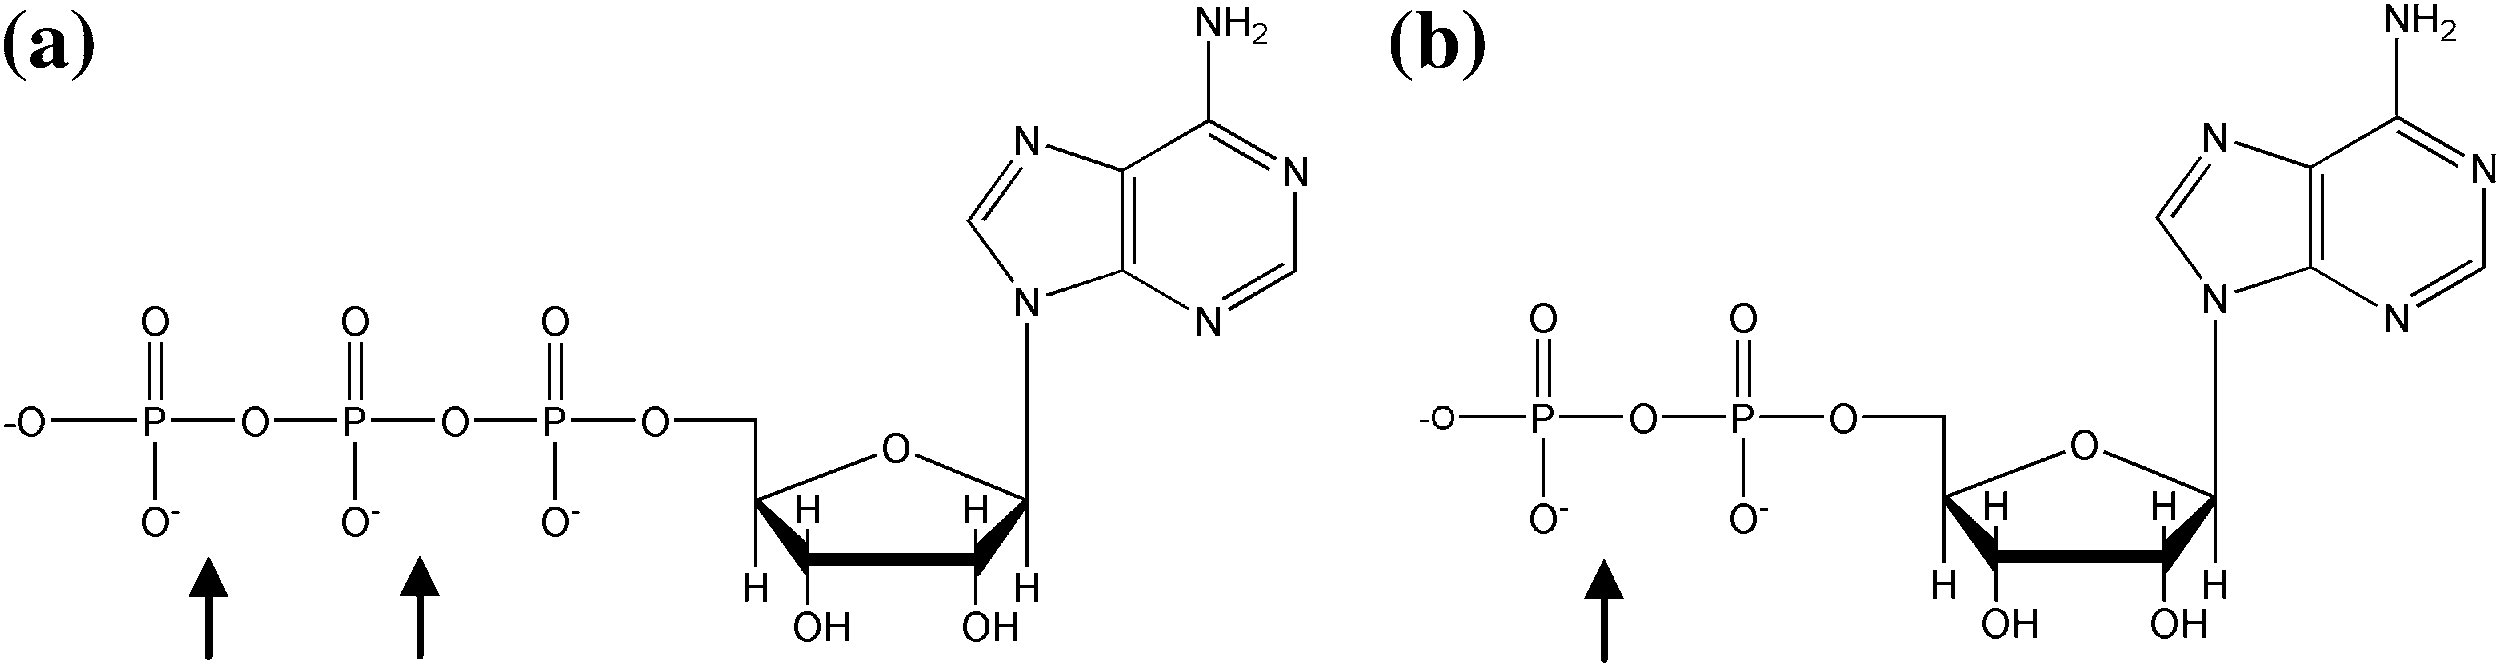
\includegraphics[width=0.8\textwidth]{63.png}
  \caption{Las estructuras de (\textbf{a}) ATP y (\textbf{b}) ADP, que muestran que el ATP tiene un grupo fosfato inorgánico $\text{P}_i$ más que el ADP. De izquierda a derecha se muestran los (\textbf{a}) tres o (\textbf{b}) dos grupos fosfato, el azúcar de cinco carbonos, la ribosa, y la adenina, que es la estructura de doble anillo. Los dos enlaces inestables de alta energía que unen los grupos fosfato en el ATP y el único enlace inestable similar en el ADP se indican con flechas.}
  \label{fig:63}
\end{figure}



La estructura del ATP se muestra en la Fig. 6.3. Consiste en un azúcar de cinco carbonos, la ribosa, que está unida a la base aromática, la adenina —formando la adenosina—, y tres grupos fosfato. Los dos enlaces que unen los grupos fosfato son enlaces inestables de alta energía; el enlace interfosfato situado más a la izquierda en la Fig. 6.3 se rompe en la hidrólisis del ATP
\begin{equation}
\text{ATP} + \text{H}_2\text{O} \rightarrow \text{ADP} + \text{fosfato inorgánico} + \text{energía},
\label{eq:613}
\end{equation}
donde el ADP es adenosín difosfato. Este es el proceso catabólico básico para la liberación de energía, y fue analizado como la fuerza motriz en el golpe de fuerza de la miosina para generar fuerza en los músculos en el Cap. 5. La energía liberada, o más precisamente la energía libre, varía de $7$ a $14\text{ kcal/mol de ATP}$, dependiendo de las condiciones (véase el Problema 6.32). Bajo condiciones celulares típicas, puede ser de $\simeq 12\text{--}14\text{ kcal/mol}$ \cite{55,63,75}.

\textbf{Anabolismo.} Después de la hidrólisis, el ADP necesita combinarse con un grupo fosfato para reformar el ATP para su uso posterior. En promedio, cada molécula de ATP se recicla de esta manera aproximadamente cada dos minutos (véase el Problema 6.38). ¿Cómo utiliza el cuerpo las fuentes de alimentos como la glucosa para hacer esto? Esto ocurre mediante una serie de pasos químicos que pueden proceder hasta cierto límite sin oxígeno (glucólisis anaeróbica) y en mayor medida con oxígeno (metabolismo aeróbico o respiración) \cite{20,35,57,75,106}. Esto utiliza la glucosa en el torrente sanguíneo y el glucógeno, $(\text{C}_6\text{H}_{12}\text{O}_6)_n$, un azúcar polimerizado de cadena ramificada que consiste en moléculas de glucosa como monómeros unidos entre sí con enlaces glucosídicos (oxígeno). El glucógeno se almacena en las células musculares, donde se utiliza directamente, y en el hígado, donde se descompone en glucosa mediante la glucogenólisis, que luego es transportada por la sangre a las otras células. En el metabolismo aeróbico, los productos de las etapas anaeróbicas se metabolizan más profundamente (en presencia de oxígeno) para completar el metabolismo de la glucosa almacenada mediante una serie compleja de pasos denominados colectivamente ciclo de Krebs y sistema de transporte de electrones (ETS); estos se muestran en la Fig. 6.4 y se describen con un poco más de detalle más adelante. El resultado general es que, en el metabolismo aeróbico, $1\text{ mol}$ de glucosa puede producir aproximadamente $30\text{--}32\text{ mol}$ de ATP (dependiendo de los detalles del mecanismo de lanzadera de la membrana). (De hecho, $1\text{ mol}$ de carbohidratos provenientes del glucógeno muscular puede producir aproximadamente $31\text{--}33\text{ mol}$ de ATP, pero se utiliza energía en la formación de glucógeno a partir de la glucosa; consideraremos únicamente el metabolismo de la glucosa). De estos, $2\text{ mol}$ se producen mediante procesos anaeróbicos y $28\text{--}30\text{ mol}$ adicionales se producen cuando hay suficiente oxígeno. El resultado final es que la hidrólisis de estos, digamos por ahora, $30\text{ mol}$ de ATP proporcionados por la glucosa
\begin{equation}
30\text{ mol de ATP/mol de glucosa} \times 14,0\text{ kcal/mol de ATP} = 420\text{ kcal/mol de glucosa}.
\label{eq:614}
\end{equation}
Esto debe compararse con la energía proveniente de la combustión de la glucosa
\begin{equation}
180\text{ g/mol de glucosa} \times 3,8\text{ kcal/g de glucosa} = 686\text{ kcal/mol de glucosa}.
\label{eq:615}
\end{equation}
Esto significa que la eficiencia del uso de glucosa por parte del cuerpo para formar energía disponible en forma de ATP es de $420\text{ kcal}/686\text{ kcal} = 61\%$; para $32\text{ mol}$ de ATP formados a partir de glucosa, esto da $448\text{ kcal}/686\text{ kcal} = 65\%$. Este rango de eficiencia de $\simeq 61\text{--}65\%$ es para condiciones en las células musculares. Para otras condiciones específicas, la energía libre del ATP puede ser un poco menor. (Esto se explora en los Problemas 6.32 y 6.33). En cualquier caso, esta eficiencia es bastante buena, aunque no es perfecta. (Es mucho mejor que la eficiencia de las máquinas térmicas típicas, que es de $\sim 10\text{--}20\%$). La eficiencia general del uso de glucosa para realizar trabajo mecánico es mucho menor debido a otros factores de eficiencia que analizaremos más adelante.

\begin{figure}[htbp]
  \centering
  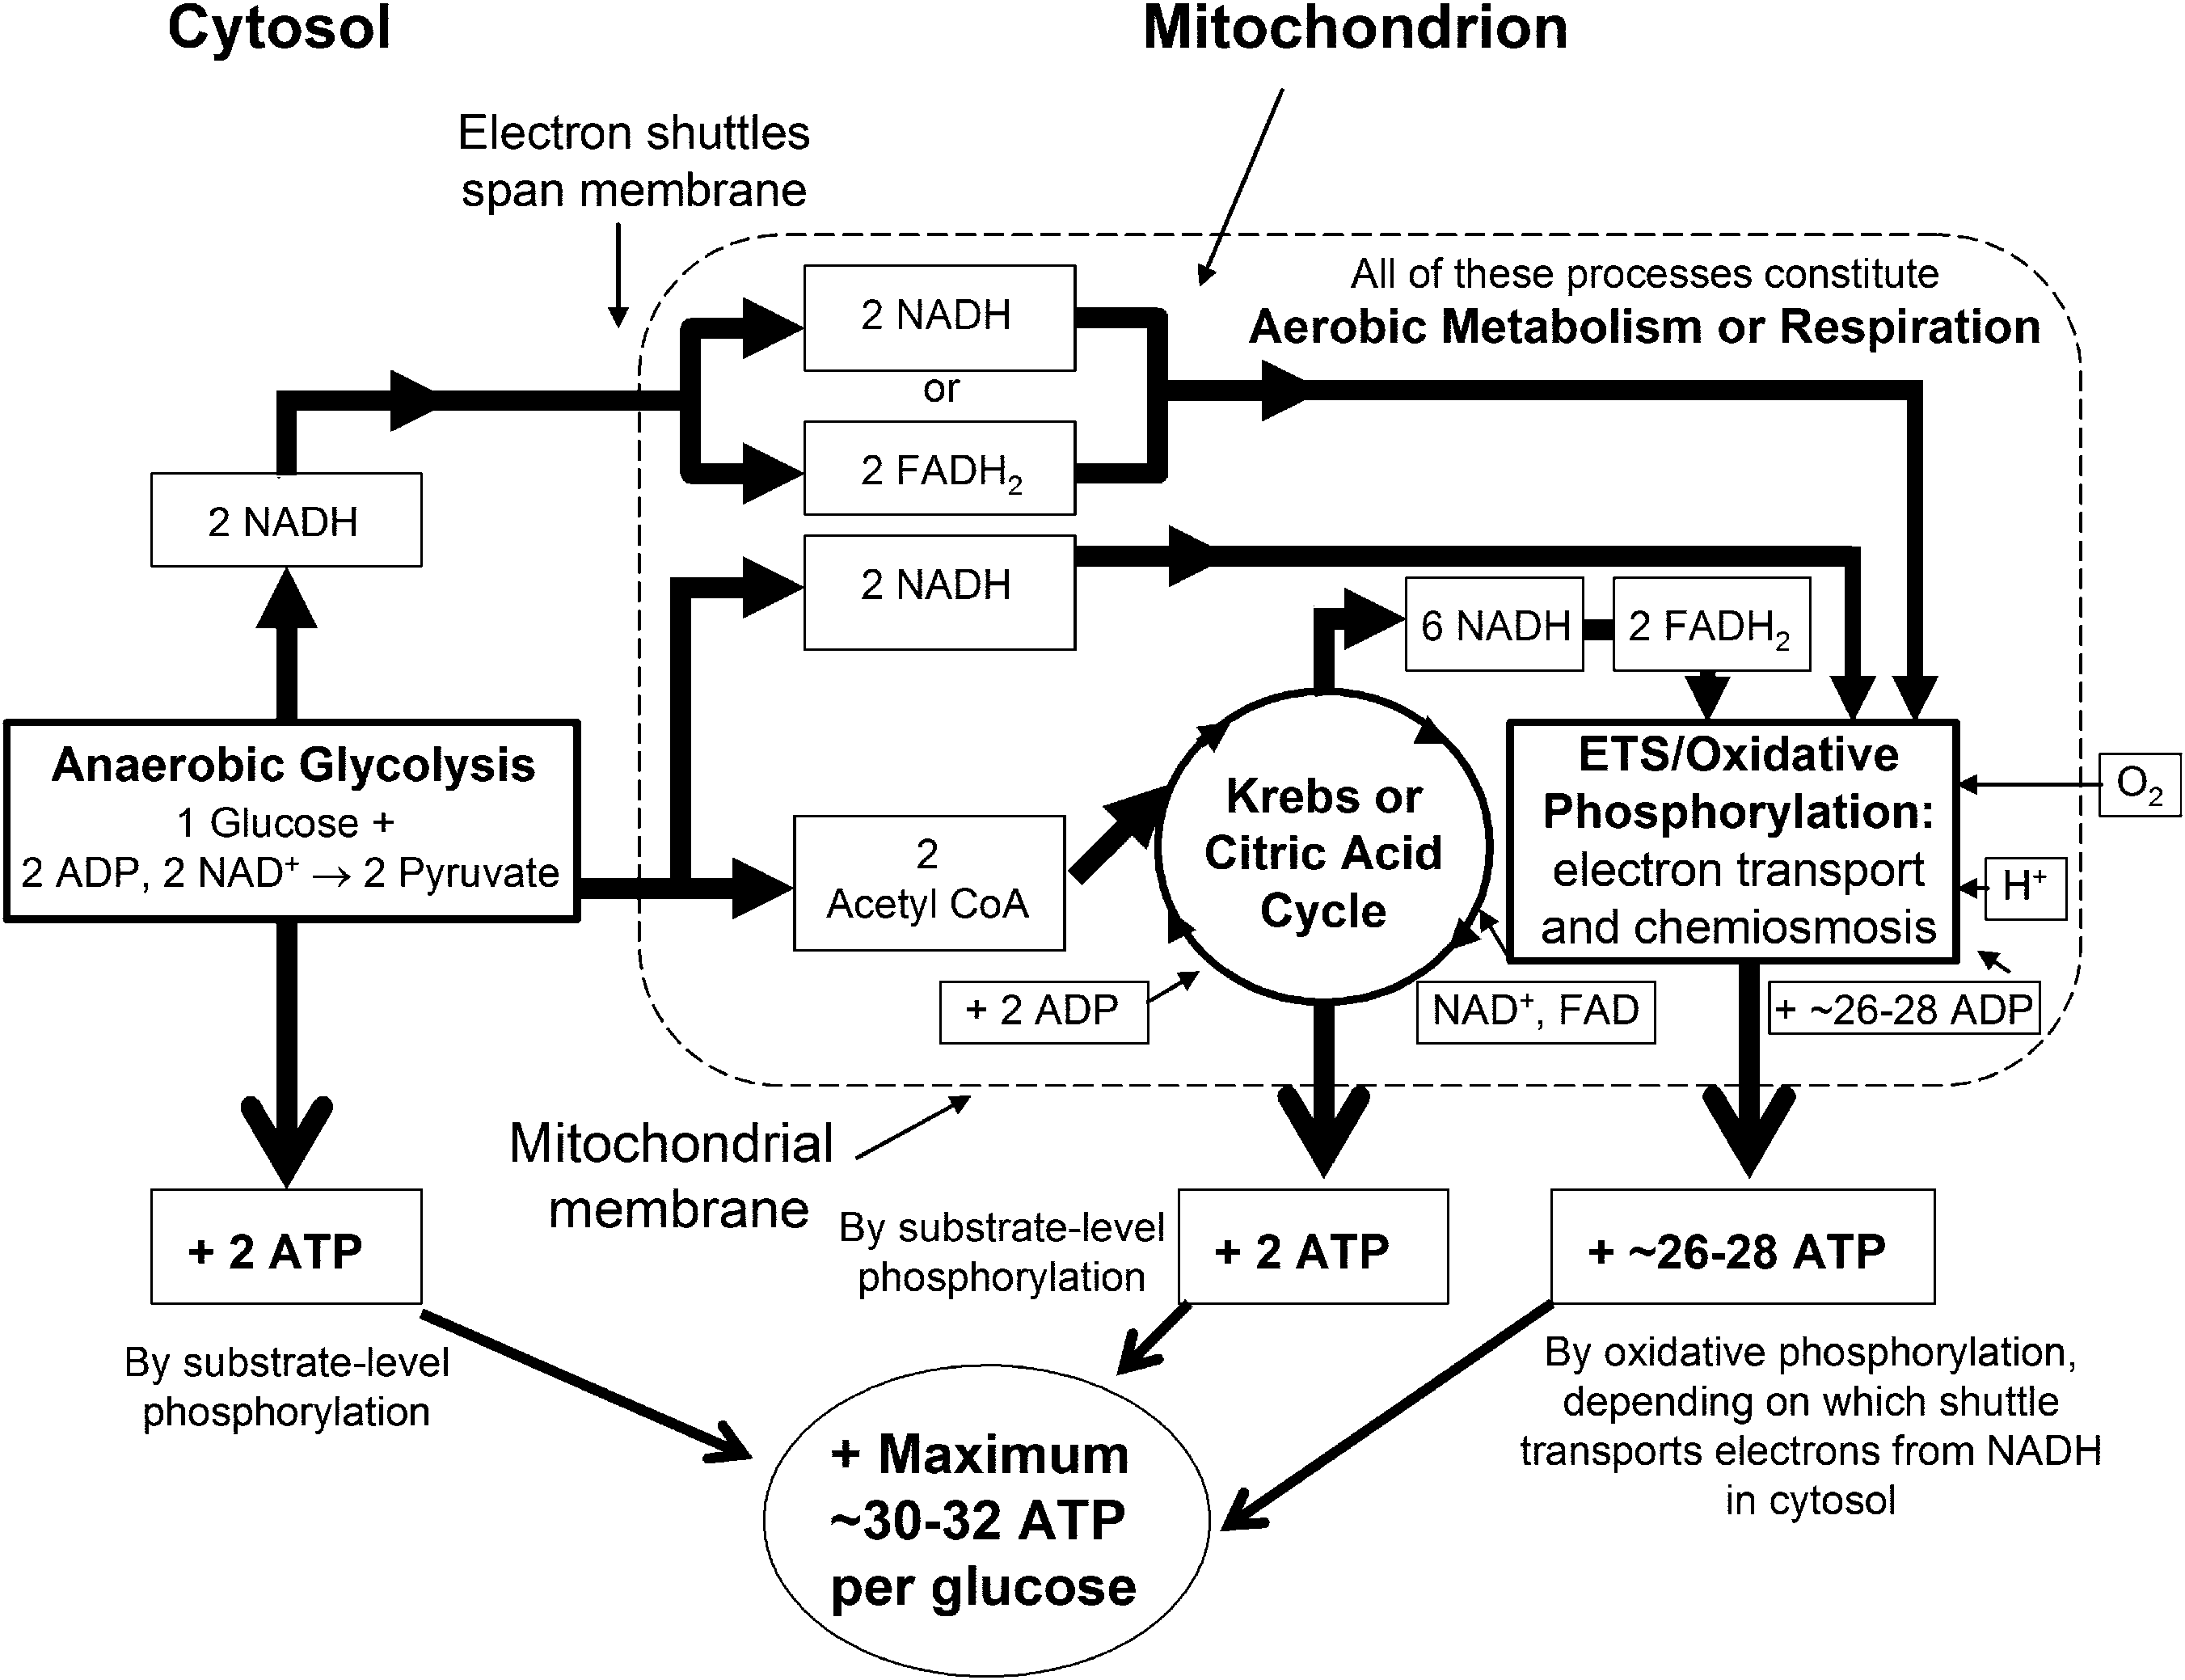
\includegraphics[width=0.7\textwidth]{64.png}
  \caption{Esquema de los procesos involucrados en la resíntesis de ATP a partir de ADP y fosfato inorgánico mediante glucólisis anaeróbica en el citosol (el fluido intracelular) y metabolismo aeróbico (o respiración) en la mitocondria (basado en \cite{20,66,75}).}
  \label{fig:64}
\end{figure}



\subsection{Cómo se utiliza realmente el ATP en el cuerpo}

El ATP es la fuente última de energía para el movimiento muscular, pero no siempre es la fuente almacenada localmente. El cuerpo tiene un mecanismo para utilizarlo directamente y luego varios niveles de mecanismos para transferir energía de otras moléculas a la formación de ATP (a partir de ADP), que luego se utiliza de forma directa. Existen cuatro niveles de etapas, cada una de las cuales puede utilizarse durante tiempos sucesivamente más largos, aunque a niveles de actividad sucesivamente menores (Tabla 6.8) \cite{35,66,75}.

\begin{table}[htbp]
\centering
\caption{Potencia y energía estimadas disponibles en el cuerpo, para un hombre de $70\text{ kg}$ con $30\text{ kg}$ de músculo, asumiendo $10\text{ kcal/mol de ATP}$}
\label{tab:68}
\small
\begin{tabularx}{\textwidth}{Xcc}
\toprule
\textbf{Sistema} & \textbf{Potencia máxima (moles de ATP/min)} & \textbf{Capacidad máxima (moles totales de ATP)} \\
\midrule
Sistema de fosfágenos (ATP-PC) & 3,6 & 0,7 \\
Glucólisis anaeróbica & $1,6\text{--}2,5$ & 1,2 \\
Metabolismo aeróbico a partir de glucógeno & 1,0 & 90,0 \\
\bottomrule
\end{tabularx}
\begin{flushleft}
    \small Utilizando datos de \cite{35}.
\end{flushleft}
\end{table}

\textbf{Paso 1.} Normalmente hay suficiente ATP en los músculos esqueléticos vivos para suministrar energía para aproximadamente $8$ sacudidas. Esto puede ser suficiente para unos $3\text{ s}$ o para aproximadamente la mitad de una carrera de $50\text{ m}$. La energía proviene de (Fig. 6.3)
\begin{equation}
\text{ATP} + \text{H}_2\text{O} \rightarrow \text{ADP} + \text{P}_i + \text{H}^+ + 14\text{ kcal/mol}.
\label{eq:616}
\end{equation}

\begin{figure}[htbp]
  \centering
  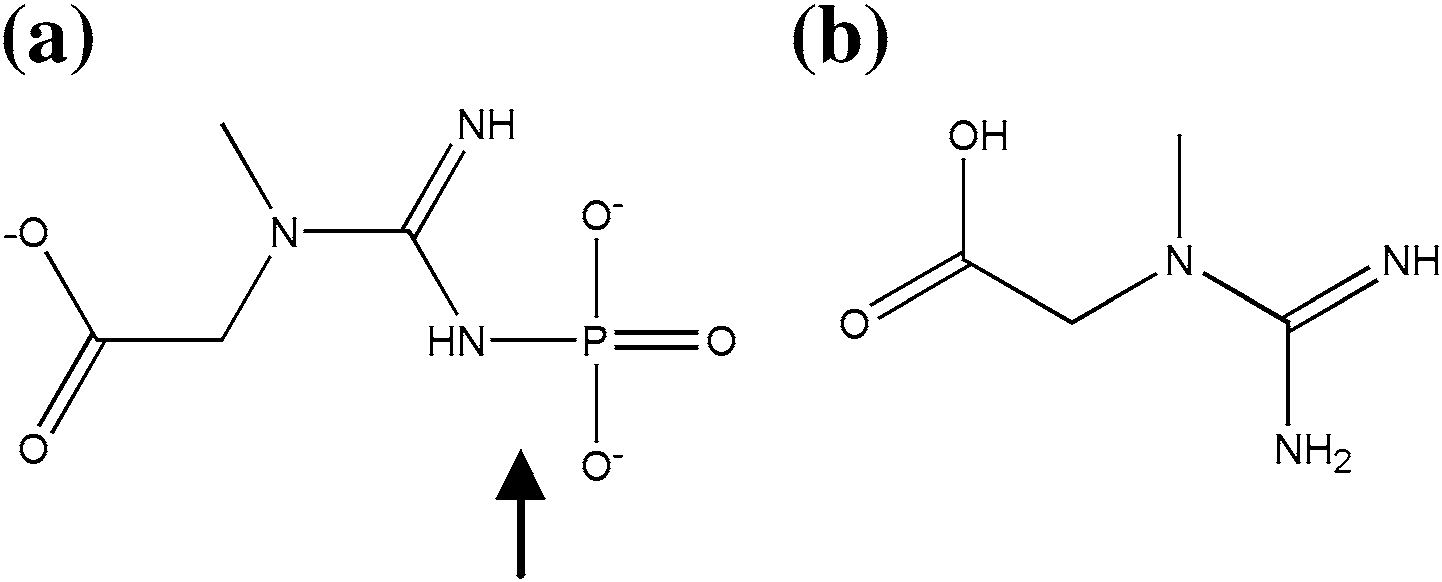
\includegraphics[width=0.8\textwidth]{65.png}
  \caption{Las estructuras de (\textbf{a}) fosfocreatina (PCr) y (\textbf{b}) creatina (Cr), que muestran que la PCr tiene un grupo fosfato inorgánico $\text{P}_i$. El enlace inestable de alta energía que une el grupo fosfato en la PCr se indica con una flecha. La enzima que cataliza la descomposición de la PCr para formar ATP, que es la transferencia del grupo fosfato de la PCr al ADP para formar ATP (\ref{eq:617}), se llama creatina quinasa.}
  \label{fig:65}
\end{figure}



\textbf{Paso 2.} Ahora se necesita más ATP. Se resintetiza a partir del depósito local de fosfocreatina (o fosfato de creatina) (PCr) (Fig. 6.5) mediante
\begin{equation}
\text{ADP} + \text{PCr} \rightarrow \text{ATP} + \text{Cr},
\label{eq:617}
\end{equation}
donde $\text{Cr}$ es creatina. Esta reacción es impulsada fuertemente hacia la derecha porque tiene una constante de equilibrio $>20$. El músculo tiene suficiente $\text{PCr}$ para proporcionar ATP para aproximadamente $\sim 100$ sacudidas, o para los primeros $50\text{ m}$ ($\sim 8\text{--}10\text{ s}$) de un sprint.

Juntos, los pasos 1 y 2 (reacciones (\ref{eq:616}) y (\ref{eq:617})) constituyen el sistema de fosfágenos o el sistema ATP-PC. Es la fuente de mayor potencia máxima, con alrededor de $4\text{ mol de ATP}$ utilizados por una persona cada minuto. Se puede utilizar durante tiempos cortos, de $8\text{--}10\text{ s}$, y a lo sumo para carreras de $100\text{ m}$ o para saltos limitados. La $\text{PCr}$ se puede reformar a partir de $\text{Cr}$ y $\text{P}_i$ utilizando el propio ATP. Para niveles intensos de ejercicio, esto puede ocurrir solo después de la actividad, y usualmente ocurre por metabolismo aeróbico.

Cuando se necesita más energía de la que puede suministrar el sistema de fosfágenos por sí solo, esta se produce a partir del glucógeno que está almacenado en el músculo y del metabolismo de la glucosa y los ácidos grasos en el torrente sanguíneo. Se producen dos moléculas de alta energía como intermediarios durante esta formación de ATP: (1) NADH (a partir de $\text{NAD}^+$, nicotinamida adenina dinucleótido, un derivado de la vitamina niacina) y (2) $\text{FADH}_2$ (a partir de FAD, flavín adenina dinucleótido, derivado de la riboflavina, una vitamina B). Los modos de utilizar estas fuentes de energía para formar ATP son diferentes para la actividad ligera y la pesada.

\textbf{Paso 3.} Durante la actividad «pesada» las personas necesitan ATP rápidamente y no hay suficiente oxígeno para el metabolismo aeróbico, por lo que solo ocurre la glucólisis anaeróbica (la vía de Embden-Meyerhof). Un mol de glucosa-1-fosfato (obtenido de $1\text{ mol}$ de carbohidratos a partir de glucógeno) puede convertir solo $3\text{ mol}$ de ADP en ATP. En este proceso, se utiliza $1\text{ mol}$ de ATP para producir fructosa-1,6-difosfato a partir de fructosa-6-fosfato (que se produce a partir de glucosa-1-fosfato), y se forman $2\text{ mol}$ de ATP en cada uno de los dos pasos subsecuentes de la glucólisis, lo que lleva a un neto de $3\text{ mol}$ de ATP. El metabolismo de la glucosa en sangre rinde un neto de solo $2\text{ mol}$ de ATP porque se necesita $1\text{ mol}$ de ATP para convertirla en glucosa-6-fosfato (véase el Problema 6.35). Todo esto ocurre en el fluido intracelular de la célula muscular (el citosol).

Esta degradación del glucógeno o de la glucosa es solo parcial, y sin suficiente oxígeno, el potencial de producir los otros $28\text{--}30\text{ mol}$ de ATP mediante los otros pasos del metabolismo aeróbico se pierde por completo. Al final de la glucólisis anaeróbica, la energía todavía está almacenada en las $2$ moléculas de ácido pirúvico ($\text{C}_3\text{H}_4\text{O}_3$) (iones piruvato en solución) formadas a partir de cada molécula de glucosa, las cuales se convierten en $2$ moléculas de ácido láctico ($\text{C}_3\text{H}_6\text{O}_3$) (iones lactato en solución) si no se pueden utilizar en el ciclo de Krebs en el metabolismo aeróbico. Además, se forman $2$ moléculas de NADH por molécula de glucosa en la glucólisis anaeróbica, y la energía de estas moléculas de alta energía también se desperdicia porque no son metabolizadas por el ETS en el metabolismo aeróbico (véase la Fig. 6.4). (Sin embargo, el NADH puede permanecer hasta que se recupere la deuda de oxígeno).

La ventaja de esta glucólisis anaeróbica o sistema de glucógeno-ácido láctico es que proporciona un nivel medio de potencia, $\sim 2,5\text{ mol de ATP/min}$, que es aproximadamente el $60\%$ de la del sistema de fosfágenos. Proporciona potencia para unas $600$ sacudidas, durante un tiempo intermedio de $\sim 1,3\text{--}1,6\text{ min}$, lo suficiente para una carrera de $400\text{ m}$. (La potencia máxima anaeróbica es de $2,1\text{ hp}$ para hombres y $1,7\text{ hp}$ para mujeres. Estos valores disminuyen drásticamente después de los $25$ años de edad). La glucólisis anaeróbica tiene desventajas. Además de ser ineficiente, produce ácido láctico, que causa malestar por acidosis y provoca fatiga. Debido a que la reacción piruvato-lactato es reversible, el ácido láctico de la glucólisis anaeróbica puede convertirse para formar piruvato cuando el oxígeno está disponible durante la recuperación del ejercicio pesado (pero principalmente en el hígado y no en el músculo).

\textbf{Paso 4.} Durante el ejercicio «ligero», hay suficiente oxígeno para que el metabolismo aeróbico complete la oxidación de los carbohidratos. El metabolismo aeróbico consta de dos procesos complejos además de la glucólisis anaeróbica: el ciclo de Krebs (que también se conoce como el ciclo del ácido tricarboxílico (TCA) o ciclo del ácido cítrico) y el sistema de transporte de electrones (ETS) (que también se conoce como la vía del citocromo o fosforilación oxidativa) (Fig. 6.4). Ambos ocurren en la mitocondria celular. Solo el ETS requiere oxígeno directamente, pero sin oxígeno incluso los beneficios del ciclo de Krebs se pierden debido a reacciones inversas. (Por cierto, Hans Adolf Krebs compartió el Premio Nobel de Fisiología o Medicina en 1953 por su descubrimiento del ciclo del ácido cítrico).

Los $2\text{ mol}$ de NADH de la glucólisis anaeróbica se transportan a través de la membrana de la mitocondria. Dos moles de piruvato de la glucólisis anaeróbica sirven como material de partida para el ciclo de Krebs. Antes de entrar en este ciclo, cada piruvato produce una molécula de acetil CoA, que entra en el ciclo de Krebs, y $1\text{ NADH}$, por lo que se producen $2\text{ acetil CoA}$ y $2\text{ NADH}$ por molécula de glucosa. Para cada piruvato, el ciclo de Krebs produce $1\text{ ATP}$, $3\text{ NADH}$ y $1\text{ FADH}_2$, junto con $2$ moléculas de $\text{CO}_2$, que son productos de desecho, por lo que para cada molécula de glucosa el ciclo de Krebs produce $2\text{ ATP}$, junto con $6$ moléculas de NADH y $2$ de $\text{FADH}_2$.

Esto significa que por cada mol de glucosa, un total de $10\text{ mol}$ de NADH y $2\text{ mol}$ de $\text{FADH}_2$ entran al ETS, donde se convierten en ATP y $\text{H}_2\text{O}$. (Alternativamente, si los $2\text{ mol}$ de NADH de la glucólisis anaeróbica transportados a través de la membrana mitocondrial se ciclan a través de la membrana como $2\text{ mol}$ de $\text{FADH}_2$, un total de $8\text{ mol}$ de NADH y $4\text{ mol}$ de $\text{FADH}_2$ entran al ETS). Existen varias series de vías alternativas en las que estas moléculas de alta energía se convierten en ATP, lo que conduce efectivamente a $2,5\text{ ATP}$ por NADH y efectivamente a $1,5\text{ ATP}$ por $\text{FADH}_2$, o $2,5 \times 10 + 1,5 \times 2 = 28\text{ mol}$ de ATP. También están los $2\text{ mol}$ de ATP directamente de la glucólisis anaeróbica y los $2\text{ mol}$ de ATP directamente del ciclo de Krebs, para un total de $32\text{ mol}$ de ATP. En general, se produce un total de $30\text{--}32\text{ mol}$ de ATP a partir de $1\text{ mol}$ de glucosa (dependiendo del mecanismo de lanzadera de la membrana). (Esta estimación de $30\text{--}32\text{ mol}$ de ATP por mol de glucosa se cita en trabajos más recientes \cite{57,75}; estimaciones más antiguas concluían que se producían de $36\text{--}38\text{ mol}$ de ATP por mol de glucosa \cite{55}).

El ATP también se forma por la oxidación de ácidos grasos y de algunos aminoácidos y proteínas. (Las grasas y las proteínas pueden ser metabolizadas solo en presencia de oxígeno). El papel del metabolismo de las proteínas es muy menor durante el reposo y no contribuye con más del $5\text{--}10\%$ del suministro total de energía durante el ejercicio normal. Cada molécula de ácido graso se activa utilizando $2$ moléculas de ATP, y luego se metaboliza en pases sucesivos a través de un ciclo metabólico dentro de la mitocondria en el cual se pierden dos átomos de carbono en cada pase para producir una molécula de acetil-CoA, NADH y $\text{FADH}_2$ mediante la $\beta$-oxidación, hasta que queda el acetil-CoA. Para el ácido palmítico de cadena de 16 carbonos, hay siete pases completos y por lo tanto un mol de ácido palmítico produce $8\text{ mol}$ de acetil-CoA (incluyendo el que queda después de la $\beta$-oxidación), $7\text{ mol}$ de NADH y $7\text{ mol}$ de $\text{FADH}_2$. Cada mol de acetil-CoA se oxida luego en el ciclo de Krebs para dar $3\text{ mol}$ de NADH, $1\text{ mol}$ de $\text{FADH}_2$ y $1\text{ mol}$ de ATP. El NADH y el $\text{FADH}_2$ entran al sistema ETS. Para el ácido palmítico, esto significa que $31\text{ mol}$ de NADH y $15\text{ mol}$ de $\text{FADH}_2$ entran al sistema ETS. En general, se forman $2,5 \times 31 + 1,5 \times 15 = 100\text{ mol}$ de ATP en el ETS. Incluyendo los otros $8\text{ mol}$ de ATP, se forman $108\text{ moles}$ de ATP por mol de ácido palmítico. Incluyendo los $2\text{ moles}$ de ATP utilizados para la activación, se forma un neto de $106\text{ moles}$ de ATP \cite{75}.

Un hombre sano con un entrenamiento adecuado puede aportar $\sim 50\text{ mL de oxígeno/kg-min}$. Este sistema aeróbico proporciona la potencia máxima más baja, $1\text{ mol de ATP/min}$ ($\sim 25\%$ de la del sistema de fosfágenos), pero durante un tiempo muy prolongado. Hay suficiente glucógeno para unas $\sim 10.000$ sacudidas. Es útil para actividades de resistencia y larga distancia, incluyendo la carrera de maratón. El glucógeno en el músculo se agota después de varias horas ($\sim 1,5\text{--}4,0\text{ h}$) de este nivel de actividad. (La glucosa en sangre también se puede convertir en ácido pirúvico y luego ser utilizada en las mitocondrias celulares en presencia de oxígeno para formar más ATP. Este es un proceso eficiente y a largo plazo).

Se almacena una cantidad insignificante de oxígeno en el cuerpo. Debe ser introducido por los pulmones y transferido a la sangre en las arterias continuamente. El oxígeno se transfiere a las células, dejando sangre desoxigenada en las venas. Podemos seguir la conservación de las moléculas de $\text{O}_2$ en el cuerpo. La tasa de consumo corporal de $\text{O}_2$, $d V_{\text{O}_2}/dt$, es igual al producto del gasto cardíaco (tasa de flujo sanguíneo, $Q_t$, véase el Cap. 8) y la diferencia en el contenido de oxígeno (presión parcial de oxígeno) en las arterias y venas, $p_a - p_v$:
\begin{equation}
\frac{d V_{\text{O}_2}}{dt} = Q_t(p_a - p_v).
\label{eq:618}
\end{equation}

Durante el ejercicio aeróbico, $d V_{\text{O}_2}/dt$ aumenta linealmente con $Q_t$. Para una persona con una condición física promedio, las tasas máximas de uso de oxígeno y de flujo sanguíneo son $(d V_{\text{O}_2}/dt)_{\text{max}} \approx 2,8\text{ L/min}$ (litros de gas oxígeno a una atmósfera) y $(Q_t)_{\text{max}} \approx 19\text{ L/min}$, y para una persona con una condición física muy alta son $\approx 4\text{ L/min}$ y $25\text{ L/min}$, respectivamente.

La Tabla 6.9 proporciona las concentraciones y cantidades totales de moléculas de almacenamiento de energía y la energía disponible a partir de ellas para un hombre de $70\text{ kg}$ con $30\text{ kg}$ de músculo. Las mujeres tienen aproximadamente las mismas concentraciones de ATP y $\text{PC}$ por kilogramo de músculo que los hombres, pero tienen menos músculo en general. Los recursos de energía química específica típicos almacenados en el cuerpo se enumeran en la Tabla 6.10.

\begin{table}[htbp]
\centering
\caption{Energía disponible estimada del cuerpo (por kg y también, entre paréntesis, total), para un hombre de $70\text{ kg}$ con $30\text{ kg}$ de músculo, asumiendo $10\text{ kcal/mol de ATP}$}
\label{tab:69}
\small
\begin{tabularx}{\textwidth}{Xcc}
\toprule
\textbf{Sistema} & \textbf{Cantidades musculares} & \textbf{Energía útil} \\
 & \textbf{(en mmol/kg de músculo$^{\text{a}}$) (total)} & \textbf{(en kcal/kg de músculo) (total)} \\
\midrule
\multicolumn{3}{l}{\textit{Sistema de fosfágenos (ATP-PC)}} \\
\quad ATP & $4\text{--}6$ ($120\text{--}180$) & $0,04\text{--}0,06$ ($1,2\text{--}1,8$) \\
\quad PC & $15\text{--}17$ ($450\text{--}510$) & $0,15\text{--}0,17$ ($4,5\text{--}5,1$) \\
\quad Total: ATP + PC & $19\text{--}23$ ($570\text{--}690$) & $0,19\text{--}0,23$ ($5,7\text{--}6,9$) \\
\midrule
\multicolumn{3}{l}{\textit{Glucólisis anaeróbica}} \\
\quad Formación de ATP & $33\text{--}38$ ($1000\text{--}1200$) & $0,33\text{--}0,38$ ($10,0\text{--}12,0$) \\
\midrule
\multicolumn{3}{l}{\textit{Metabolismo aeróbico}} \\
\quad A partir de glucógeno almacenado & $13\text{--}15\text{ g}$ ($400\text{--}450$) & -- \\
\quad Formación de ATP & $2800\text{--}3200$ ($87\,000\text{--}98\,000$) & $28\text{--}32$ ($870\text{--}980$) \\
\bottomrule
\end{tabularx}
\begin{flushleft}
    $^{\text{a}}$ A menos que se indique lo contrario.\\
    Utilizando datos de \cite{35}.
\end{flushleft}
\end{table}

La Tabla 6.11 enumera el sistema de energía que se utiliza principalmente en diversas actividades deportivas. Esto se explora con más detalle en la Tabla 6.12, que proporciona la fracción de cada sistema utilizado en diferentes actividades deportivas. Estas fracciones se dan para distancias más cortas y más largas en patinaje de velocidad sobre hielo, natación y carrera a pie en las Tablas 6.13, 6.14 y 6.15.

\begin{table}[htbp]
\centering
\caption{Reservas corporales de combustible y energía, para una persona de $65\text{ kg}$ ($143\text{ lb}$) con $12\%$ de grasa corporal}
\label{tab:610}
\small
\begin{tabularx}{0.8\textwidth}{Xcc}
\toprule
 & \textbf{Cantidad (g)} & \textbf{Energía (kcal)} \\
\midrule
\multicolumn{3}{l}{\textit{Carbohidratos}} \\
Glucógeno hepático & 110 & 451 \\
Glucógeno muscular & 500 & 2050 \\
Glucosa en fluidos corporales & 15 & 62 \\
\textbf{Total de carbohidratos} & \textbf{625} & \textbf{2563} \\
\midrule
\multicolumn{3}{l}{\textit{Grasa}} \\
Subcutánea y visceral & 7800 & $73\,320$ \\
Intramuscular & 161 & 1513 \\
\textbf{Total de grasa} & \textbf{7961} & \textbf{74\,833} \\
\bottomrule
\end{tabularx}
\begin{flushleft}
    \small Utilizando datos de \cite{106}.
\end{flushleft}
\end{table}

\begin{table}[htbp]
\centering
\caption{Sistemas de energía utilizados en deportes}
\label{tab:611}
\small
\begin{tabularx}{\textwidth}{l X}
\toprule
\textbf{Sistema de energía} & \textbf{Actividades deportivas} \\
\midrule
\textbf{Principalmente sistema de fosfágenos} & Carrera de $100\text{ m}$, saltos, levantamiento de pesas, clavados, sprints en fútbol americano. \\
\midrule
\textbf{Sistemas de fosfágenos y de glucógeno-ácido láctico} & Carrera de $200\text{ m}$, baloncesto, home run en béisbol (correr alrededor de las bases), sprints en hockey sobre hielo. \\
\midrule
\textbf{Principalmente sistema de glucógeno-ácido láctico} & Carrera de $400\text{ m}$, $100\text{ m}$ de natación, tenis, fútbol. \\
\midrule
\textbf{Sistemas de glucógeno-ácido láctico y aeróbicos} & Carrera de $800\text{ m}$, $200\text{ m}$ y $400\text{ m}$ de natación, $1500\text{ m}$ de patinaje, boxeo, $2000\text{ m}$ de remo, carrera de $1500\text{ m}$ / $1\text{ milla}$. \\
\midrule
\textbf{Sistemas aeróbicos} & $10\,000\text{ m}$ de patinaje, esquí de fondo, carrera de maratón ($26,2\text{ millas}$, $42,2\text{ km}$), trote. \\
\bottomrule
\end{tabularx}
\begin{flushleft}
    \small Utilizando datos de \cite{45}.
\end{flushleft}
\end{table}

En cada caso, los sprints de corta distancia utilizan los sistemas ATP-PC y anaeróbico, mientras que los eventos de mayor distancia utilizan principalmente el sistema aeróbico.

Los pasos metabólicos involucrados en estos sistemas están todos regulados por un mecanismo de retroalimentación y control (Cap. 13), y van seguidos de una etapa de recuperación. La Tabla 6.16 proporciona el tiempo de recuperación para restablecer las reservas de energía en reposo y el $\text{O}_2$, y para reducir el ácido láctico después del ejercicio. El ejercicio anaeróbico está limitado por la tolerancia máxima al ácido láctico, que es de aproximadamente $2,0\text{--}2,3\text{ g/kg de músculo}$, por lo que esto equivale a $60\text{--}70\text{ g}$ para $30\text{ kg}$ de músculo. Se puede aprender un poco sobre la etapa de recuperación corriendo tan rápido como se pueda durante el mayor tiempo posible. Entonces se estará jadeando y resoplando, respirando aire lo más rápido posible. Esto es parte de la recuperación. (Consulte a su médico antes de intentar esta demostración).

\begin{table}[htbp]
\centering
\caption{Porcentaje de énfasis de los sistemas de energía}
\label{tab:612}
\small
\begin{tabularx}{\textwidth}{X >{\centering\arraybackslash}c >{\centering\arraybackslash}c >{\centering\arraybackslash}c}
\toprule
\textbf{Deporte o actividad} & \textbf{ATP-PC y glucólisis} & \textbf{Glucólisis anaeróbica} & \textbf{Aeróbica} \\
 & \textbf{anaeróbica (\%)} & \textbf{y aeróbica (\%)} & \textbf{(\%)} \\
\midrule
Danza aeróbica (aeróbic) & 5 & 15\text{--}20 & 75\text{--}80 \\
Béisbol & 80 & 15 & 5 \\
Baloncesto & 60 & 20 & 20 \\
Clavados & 98 & 2 & Despreciable \\
Esgrima & 90 & 10 & Despreciable \\
Hockey sobre césped & 50 & 20 & 30 \\
Fútbol americano & 90 & 10 & Despreciable \\
Golf & 95 & 5 & Despreciable \\
Gimnasia & 80 & 15 & 5 \\
Hockey sobre hielo & & & \\
\quad Delantero, defensa & 60 & 20 & 20 \\
\quad Portero & 90 & 5 & 5 \\
Lacrosse & & & \\
\quad Portero, defensa, atacante & 50 & 20 & 30 \\
\quad Mediocampistas, en desventaja & 60 & 20 & 20 \\
Remo & 20 & 30 & 50 \\
Fútbol & & & \\
\quad Portero, extremos, delanteros & 60 & 30 & 10 \\
\quad Mediocampistas o líbero & 60 & 20 & 20 \\
Máquina de step & 5 & 25 & 70 \\
Tenis & 70 & 20 & 10 \\
Pruebas de campo (atletismo) & 95\text{--}98 & 2\text{--}5 & Despreciable \\
Voleibol & 80 & 5 & 15 \\
Caminar & Despreciable & 5 & 95 \\
Lucha & 90 & 5 & 5 \\
\bottomrule
\end{tabularx}
\begin{flushleft}
    \small Utilizando datos de \cite{35,36}.
\end{flushleft}
\end{table}

\begin{table}[htbp]
\centering
\caption{Porcentaje de énfasis de los sistemas de energía para un rango de distancias en patinaje de velocidad sobre hielo}
\label{tab:613}
\small
\begin{tabularx}{\textwidth}{X >{\centering\arraybackslash}c >{\centering\arraybackslash}c >{\centering\arraybackslash}c}
\toprule
\textbf{Actividad} & \textbf{ATP-PC y glucólisis} & \textbf{Glucólisis anaeróbica} & \textbf{Aeróbica} \\
 & \textbf{anaeróbica (\%)} & \textbf{y aeróbica (\%)} & \textbf{(\%)} \\
\midrule
\textit{Patinaje de velocidad sobre hielo} & & & \\
\quad $500\text{ m}$ & 80 & 10 & 10 \\
\quad $1000\text{ m}$ & 35 & 55 & 10 \\
\quad $1500\text{ m}$ & 20\text{--}30 & 30 & 40\text{--}50 \\
\quad $5000\text{ m}$ & 10 & 25 & 65 \\
\quad $10\,000\text{ m}$ & 5 & 15 & 80 \\
\midrule
\textit{Patinaje en línea} & & & \\
\quad $>10\text{ km}$ & 5 & 25 & 70 \\
\bottomrule
\end{tabularx}
\begin{flushleft}
    \small Utilizando datos de \cite{35,36}.
\end{flushleft}
\end{table}

\begin{table}[htbp]
\centering
\caption{Porcentaje de énfasis de los sistemas de energía para un rango de distancias en natación}
\label{tab:614}
\small
\begin{tabularx}{\textwidth}{X >{\centering\arraybackslash}c >{\centering\arraybackslash}c >{\centering\arraybackslash}c}
\toprule
\textbf{Natación} & \textbf{ATP-PC y glucólisis} & \textbf{Glucólisis anaeróbica} & \textbf{Aeróbica} \\
 & \textbf{anaeróbica (\%)} & \textbf{y aeróbica (\%)} & \textbf{(\%)} \\
\midrule
$50\text{ m}$ & 90 & 5 & 5 \\
$100\text{ m}$ & 80 & 15 & 5 \\
$200\text{ m}$ & 30 & 65 & 5 \\
$400\text{ m}$ & 20 & 40 & 40 \\
$1500\text{ m}$ & 10 & 20 & 70 \\
\bottomrule
\end{tabularx}
\begin{flushleft}
    \small Utilizando datos de \cite{35,36}.
\end{flushleft}
\end{table}

\begin{table}[htbp]
\centering
\caption{Porcentaje de énfasis de los sistemas de energía para un rango de distancias en carrera a pie}
\label{tab:615}
\small
\begin{tabularx}{\textwidth}{X >{\centering\arraybackslash}c >{\centering\arraybackslash}c >{\centering\arraybackslash}c}
\toprule
\textbf{Carrera a pie} & \textbf{ATP-PC y glucólisis} & \textbf{Glucólisis anaeróbica} & \textbf{Aeróbica} \\
 & \textbf{anaeróbica (\%)} & \textbf{y aeróbica (\%)} & \textbf{(\%)} \\
\midrule
$100$, $200\text{ m}$ & 95\text{--}98 & 2\text{--}5 & Despreciable \\
$400\text{ m}$ & 80 & 15 & 5 \\
$800\text{ m}$ & 30 & 65 & 5 \\
$1500\text{ m}$ (o milla) & 20\text{--}30 & 20\text{--}30 & 40\text{--}60 \\
$3000\text{ m}$ (o $2\text{ millas}$) & 10 & 20 & 70 \\
$5000\text{ m}$ (o $3\text{ millas}$) & 10 & 20 & 70 \\
$10\,000\text{ m}$ (o $6\text{ millas}$) & 5 & 15 & 80 \\
Maratón & Despreciable & 5 & 95 \\
\bottomrule
\end{tabularx}
\begin{flushleft}
    \small Utilizando datos de \cite{35,36}.
\end{flushleft}
\end{table}

\begin{table}[htbp]
\centering
\caption{Tiempos de recuperación después de un ejercicio exhaustivo}
\label{tab:616}
\small
\begin{tabularx}{\textwidth}{Xcc}
\toprule
 & \textbf{Mínimo} & \textbf{Máximo} \\
\midrule
Restauración de fosfágenos ($\text{ATP} + \text{PC}$) & $2\text{ min}$ & $5\text{ min}$ \\
Reabastecimiento de glucógeno muscular & $5\text{--}10\text{ h}$ & $24\text{--}46\text{ h}$ \\
Reabastecimiento de glucógeno hepático & Desconocido & $12\text{--}24\text{ h}$ \\
Restauración de $\text{O}_2$ en plasma y mioglobina & $10\text{--}15\text{ s}$ & $1\text{ min}$ \\
Duración del componente rápido de la recuperación de $\text{O}_2$ & $3\text{ min}$ & $6\text{ min}$ \\
Duración del componente lento de la recuperación de $\text{O}_2$ & $30\text{ min}$ & $1\text{ h}$ \\
Reducción de ácido láctico en sangre y músculo & $30\text{--}60\text{ min}^{\text{a}}$ & $1\text{--}2\text{ h}^{\text{a}}$ \\
\bottomrule
\end{tabularx}
\begin{flushleft}
    \small $^{\text{a}}$ Recuperación más rápida con ejercicio y más lenta con descanso.\\
    Utilizando datos de \cite{35}.
\end{flushleft}
\end{table}

\section{Tasas metabólicas}

Existen variaciones entre las tasas metabólicas (TM) de las personas debido a sus diferentes pesos, genética, etc. Las necesidades metabólicas a lo largo de los años han cambiado, en parte debido a los cambios en las estaturas y pesos corporales, y en los niveles de actividad \cite{34}. Primero, discutiremos las tasas metabólicas mínimas para las personas y luego abordaremos cómo la actividad incrementa la tasa metabólica. La tasa metabólica también puede depender de la ingesta de alimentos. Por ejemplo, se sabe que la TM disminuye bajo condiciones de ayuno y este cambio contrarresta algunos de los efectos esperados de las dietas. Aunque se denominan ampliamente tasas metabólicas, estas son más precisamente tasas catabólicas. A veces, la TM se denomina gasto energético total, TEE (por sus siglas en inglés), lo que podría dejar más claro que la ingesta calórica que no se gasta como energía es almacenada por el cuerpo.

\subsection{Tasa metabólica basal (BMR)}

La tasa metabólica basal (BMR) es la de un cuerpo inactivo y despierto. La BMR para una persona de $70\text{ kg}$ es de aproximadamente $1680\text{ kcal/día} \simeq 70\text{ kcal/h} \simeq 81\text{ W}$. Esto significa que, incluso en reposo, cada uno de nosotros emite casi la misma cantidad de calor que una bombilla incandescente de $100\text{ W}$. Como veremos más adelante, cuanto más pesada sea la persona, mayor será la BMR. Aproximadamente el $85\%$ de las personas del mismo género y peso tienen una BMR dentro del $6\text{--}10\%$ de la media para su clasificación (Tabla 6.14).

Los números exactos que se encuentran para la BMR a veces varían con la fuente. Esto puede debido en parte a las exigentes condiciones utilizadas para definir la BMR y a la falta de especificación del género, edad, peso, etc., de la persona. Para medir su BMR, usted debe:
\begin{enumerate}[label={(\arabic*)}]
  \item No haber consumido alimentos durante al menos $12\text{ h}$.
  \item Haber tenido una noche de sueño reparador y ninguna actividad extenuante posterior.
  \item Estar descansando completamente en posición reclinada durante al menos $30\text{ min}$.
  \item No experimentar ninguna excitación por factores psíquicos o físicos.
  \item Estar en una habitación con una temperatura de $20$ a $27^\circ\text{C}$ ($68$ a $80^\circ\text{F}$).
\end{enumerate}

La BMR es mayor que la tasa metabólica durante el sueño (cuando hay una digestión mínima de alimentos). Debido a la naturaleza estricta de las pruebas de BMR, las tasas metabólicas «de fondo» o «mínimas» a veces se prueban bajo condiciones algo menos exigentes, y estas tasas medidas no se citan como BMR, sino que se denominan de manera diferente, aunque no siempre de forma uniforme. El gasto energético basal (BEE) a menudo se define como equivalente a la BMR. La tasa metabólica en reposo (RMR) es similar a la BMR, pero se mide bajo condiciones algo menos restrictivas —temprano en la mañana después de un ayuno nocturno y $8\text{ h}$ de sueño—, por lo que es más fácil de lograr y, por lo tanto, se usa a menudo. El gasto energético en reposo (REE) generalmente se mide después de $4\text{ h}$ de estar sentado y es un poco mayor que la BMR. La BMR y las tasas metabólicas durante las actividades a menudo se determinan midiendo la ingesta de oxígeno, porque son proporcionales entre sí para las actividades aeróbicas.

\begin{table}[htbp]
\centering
\caption{Metabolismo de una persona en reposo}
\label{tab:617}
\small
\begin{tabularx}{0.8\textwidth}{X >{\centering\arraybackslash}c >{\centering\arraybackslash}c >{\centering\arraybackslash}c}
\toprule
\textbf{Sistema} & \textbf{Porcentaje} & \textbf{Tasa met.} & \textbf{Masa del órgano (kg)} \\
 & \textbf{de la BMR (\%)} & \textbf{(kcal/min)} & \textbf{para un hombre de $65\text{ kg}$} \\
\midrule
Hígado y bazo & 27 & 0,33 & -- \\
Cerebro & 19 & 0,23 & 1,40 \\
Músculo esquelético & 18 & 0,22 & 28,0 \\
Riñón & 10 & 0,13 & 0,30 \\
Corazón & 7 & 0,08 & 0,32 \\
Resto & 19 & 0,23 & -- \\
\midrule
\textbf{Suma} & \textbf{100} & \textbf{1,22} & \textbf{--} \\
\bottomrule
\end{tabularx}
\begin{flushleft}
    \small Utilizando datos de \cite{19}.
\end{flushleft}
\end{table}

El funcionamiento de varios órganos contribuye a esta BMR en una persona en reposo, como se observa en la Tabla 6.17. Tres cuartas partes de la actividad metabólica ocurren en órganos con una masa total de $5\text{ kg}$, lo cual representa el $\sim 8\%$ de la masa corporal total. Estimaremos estas tasas metabólicas del corazón y los pulmones en los Caps. 8 y 9.

Los cerebros humanos y los sistemas gastrointestinales (que no se enumeran en la Tabla 6.17) tienen aproximadamente la misma masa y tasas metabólicas, por lo que requieren aproximadamente la misma energía por unidad de masa, $\sim 11\text{--}12\text{ W/kg}$. Nuestros cerebros son mucho más grandes y nuestros sistemas gastrointestinales son mucho más pequeños que los de los primates y otros mamíferos, como se espera del escalamiento alométrico de la masa (aunque nuestros hígados y riñones son del tamaño esperado). Nuestros tractos gastrointestinales, más pequeños de lo esperado y, por lo tanto, con menor demanda de energía, son suficientes porque los humanos pueden adquirir y consumir fácilmente alimentos de alto valor calórico que podemos digerir rápidamente, en parte porque no tienen un contenido de fibra extremadamente alto y pueden ser procesados (es decir, cocinados). Nuestros cerebros son más grandes de lo esperado y, por lo tanto, tienen una mayor demanda energética. Quizás, debido a tractos gastrointestinales más pequeños, los humanos pueden «permitirse» energéticamente tener cerebros muy grandes \cite{3,56} (y, en equilibrio, seguir teniendo necesidades metabólicas basales generales consistentes con las esperadas del escalamiento alométrico de la BMR con la masa corporal, que discutiremos pronto).

La BMR es una función de la masa, la estatura y el género, como veremos más adelante en este capítulo. También es una función de la temperatura corporal. Cambia aproximadamente un $10\%$ (algunos dicen que un $13\%$) por cada $1^\circ\text{C}$ de cambio en la temperatura corporal. En consecuencia, la BMR aumenta un $30\%$ (o un $39\%$) cuando la temperatura corporal se eleva desde los normales $37^\circ\text{C}$ ($98,6^\circ\text{F}$) hasta $40^\circ\text{C}$ ($104,0^\circ\text{F}$), y disminuye un $30\%$ (o un $39\%$) cuando la temperatura corporal desciende desde la normal hasta $34^\circ\text{C}$ ($93,2^\circ\text{F}$).

\begin{table}[htbp]
\centering
\caption{BMR determinada para varios mamíferos}
\label{tab:618}
\small
\begin{tabularx}{0.8\textwidth}{Xcc}
\toprule
\textbf{Especie} & \textbf{Masa} & \textbf{BMR (kcal/día)} \\
\midrule
Ratón & $20\text{ g}$ & 3 \\
Mujer de referencia ($25\text{ años}$) & $55\text{ kg}$ & 1260 \\
Hombre de referencia ($25\text{ años}$) & $65\text{ kg}$ & 1500 \\
Elefante & $5000\text{ kg}$ & 70\,000 \\
\bottomrule
\end{tabularx}
\begin{flushleft}
    \small Véase, por ejemplo, \cite{66}.
\end{flushleft}
\end{table}

\subsubsection*{Escalamiento de la BMR}

Antes de abordar cómo la BMR y la TM dependen del género, el peso, la edad, etc., ampliaremos temporalmente nuestra discusión de la BMR de los humanos a todos los mamíferos. Cuanto más grande es el animal, mayor es la tasa metabólica (catabólica), lo cual es de esperar. Además, existe una forma en que la BMR se escala con un atributo físico de tamaño, específicamente la masa corporal $m_{\text{b}}$.

La Tabla 6.18 muestra que la BMR de los mamíferos aumenta sublinealmente con $m_{\text{b}}$. Muchos piensan que la variación para los mamíferos es proporcional a la potencia de $3/4$:
\begin{equation}
\text{BMR} = c m_{\text{b}}^{3/4},
\label{eq:619}
\end{equation}
donde $c \approx 90\text{ kcal/kg}^{3/4}\text{-día}$. Esto se conoce como la Ley de Kleiber [51--53], y es un ejemplo de una relación alométrica, como se describe en la Tabla 1.13. Es válida desde ratones hasta elefantes y, algunos dicen, hasta ballenas. (La novela de Steinbeck fue válida solo de ratones a hombres. En cuanto a las ballenas: existe una gran incertidumbre sobre la BMR de las ballenas. ¿Cómo se mide?) Aunque esta relación de escalamiento se desarrolló originalmente para comparar diferentes especies, funciona bastante bien de manera intraespecífica para los humanos, desde niños hasta adultos. Otros afirman que las BMR de los mamíferos aumentan con la masa a la potencia de $2/3$. Quienes creen en la Ley de Kleiber señalan que esta otra regla de escalamiento tiene un error por un factor de dos desde ratones hasta vacas.

Ambas dependencias dan esencialmente la misma predicción sobre el rango de masa de los humanos, por lo que importa poco cuál usemos para el análisis. Los partidarios de ambas reglas afirman que los datos disponibles de BMR las respaldan. En cualquier caso, es interesante examinar las razones físicas expuestas para apoyar las reglas de escalamiento de $m_{\text{b}}^{2/3}$ y $m_{\text{b}}^{3/4}$ \cite{27,42}.

Hay tanto un razonamiento físico sólido como otro bastante cuestionable en ambos conjuntos de argumentos.

\paragraph*{Apoyo a la regla de escalamiento $m_{\text{b}}^{3/4}$ de Kleiber}

Se supone que la tasa metabólica, y la BMR en particular, se escalan como la potencia máxima de salida de los músculos \cite{65,66}. El uso de potencia es proporcional a $Fv$, donde $F$ es la fuerza muscular y $v$ es la velocidad de contracción muscular. La fuerza muscular es $F = \sigma(\text{PCA})$, donde $\sigma$ es la fuerza muscular por unidad de área y $\text{PCA}$ es el área de sección transversal del músculo. Por lo tanto,
\begin{equation}
\text{BMR} \propto Fv = \sigma(\text{PCA})v.
\label{eq:620}
\end{equation}

Los estudios demuestran que para los músculos de todas las especies y tamaños, $v$ y $\sigma$ no varían sustancialmente, por lo que
\begin{equation}
\text{BMR} \propto \text{PCA}.
\label{eq:621}
\end{equation}

Si las extremidades de los mamíferos, que por supuesto contienen muchos de estos músculos, tienen un ancho característico $d$ y una longitud $L$, este área y la masa del mamífero $m_{\text{b}}$ se escalan como
\begin{equation}
\text{PCA} \propto d^2
\label{eq:622}
\end{equation}
y
\begin{equation}
m_{\text{b}} \propto d^2 L.
\label{eq:623}
\end{equation}

Para relacionar la BMR con la masa, necesitamos relacionar $L$ con $d$. Se han expuesto cuatro argumentos que sugieren que $L$ se escala con $d^{2/3}$. Primero, los datos experimentales en primates muestran que $L$ varía con $d$ de esta manera. Segundo, esta ley de escalamiento también relaciona la altura de un árbol $L$ con el ancho del tronco del árbol $d$, por lo que esta ley de escalamiento parece ser universal. Tercero, $L \propto d^{2/3}$ es también la ley de escalamiento para la condición bajo la cual una columna vertical larga de altura $L$ y ancho $d$ se pandea bajo su propio peso cuando se desplaza de la orientación vertical.

Un cuarto argumento se basa en la autosemejanza, utilizando la expresión que derivamos anteriormente, (4.46). El extremo de la viga de longitud $L$ y dimensión lateral $d$ en la Fig. 4.40 se deflecta hacia abajo una distancia $y(L) = -FL^3/3Y I_{\text{A}}$ cuando se aplica una fuerza $F$ en su extremo. Aunque el momento de inercia de área es diferente para diferentes secciones transversales —$I_{\text{A}} = \pi d^4/64$ para cilindros (a partir de $I_{\text{A}} = \pi a^4/4$ para una sección transversal circular de radio $a = d/2$ utilizando (4.42)) y $d^4/12$ para sólidos rectangulares con una sección transversal cuadrada (a partir de $I_{\text{A}} = wh^3/12$ para una sección transversal rectangular de ancho $w$ y altura $h$ —aquí con $d = w = h$, utilizando (4.41))— no hace ninguna diferencia cuál utilicemos porque ambos tienen la misma dependencia con $d^4$. (Utilizaremos formalmente la sección transversal circular).

Este ángulo de deflexión hacia abajo $\theta$ es $\sim |y|/L$, lo que da
\begin{equation}
\theta = \frac{|y|}{L} = \frac{F L^2}{3 Y I_{\text{A}}}.
\label{eq:624}
\end{equation}

La autosemejanza sugiere que $\theta$ sería el mismo para todas las especies y, en consecuencia, igual a una constante. Si $F$ se debe a la gravedad, entonces $F = m_{\text{b}}g = \rho V g$, donde $\rho$ es la densidad de masa de la viga y $V$ es su volumen $= (\pi d^2/4)L$. Si esta fuerza actuara completamente en el extremo, entonces
\begin{equation}
\theta = \frac{(\rho((\pi d^2/4)L)g)L^2}{3Y(\pi d^4/64)} = \frac{16}{3} \frac{\rho g}{Y} \frac{L^3}{d^2}.
\label{eq:625}
\end{equation}

Si $\theta$ fuera independiente de $L$ y $d$, obtenemos nuevamente $L \propto d^{2/3}$.

En cualquier caso, dado que $m_{\text{b}} \propto d^2 L$ y $L \propto d^{2/3}$, vemos que $m_{\text{b}} \propto d^2(d^{2/3}) = d^{8/3}$. Por lo tanto, $d \propto m_{\text{b}}^{3/8}$. Con $\text{BMR} \propto \text{PCA}$ y $\text{PCA} \propto d^2$, encontramos que $\text{BMR} \propto d^2$. Utilizando $d \propto m_{\text{b}}^{3/8}$, vemos que
\begin{equation}
\text{BMR} \propto \left(m_{\text{b}}^{3/8}\right)^2 = m_{\text{b}}^{3/4},
\label{eq:626}
\end{equation}
la cual es la Ley de Kleiber.

Existen muchas lagunas en este razonamiento. Por ejemplo, la potencia necesaria para hacer funcionar los músculos esqueléticos es en realidad una pequeña fracción de la BMR (Tabla 6.17), por lo que las leyes de escalamiento basadas en esta potencia pueden no representar las de toda la BMR.

\paragraph*{Apoyo a la regla de escalamiento $m_{\text{b}}^{2/3}$}

El argumento anterior asumía que la BMR se escalaba según las necesidades de potencia metabólica. Esta línea de razonamiento sostiene que la BMR está limitada por la tasa de pérdida de calor del mamífero. Un mamífero tiene un área de sección transversal que se escala como $L^2$, donde $L$ es su dimensión característica, mientras que su volumen y, por lo tanto, su masa $m_{\text{b}}$ se escalan como $L^3$. La pérdida de calor se escala como el área superficial disponible $A$, la cual varía claramente como $m_{\text{b}}^{2/3}$, por lo que
\begin{equation}
\text{BMR} \propto m_{\text{b}}^{2/3}.
\label{eq:627}
\end{equation}

\subsubsection*{Escalamiento de la BMR en humanos}

La BMR en humanos depende de la masa, así como de otros factores, como el género, la estatura y la edad. La BMR para hombres de $20\text{--}39\text{ años}$ de edad en climas de temperatura moderada oscila entre $1350$ y $2000\text{ kcal/día}$ para rangos comunes de estaturas y pesos \cite{34}.

Las ecuaciones de Harris--Benedict se utilizan comúnmente para caracterizar las BMR humanas medidas:
Para hombres:
\begin{equation}
\text{BMR} = 66{,}4730 + 13{,}7516 m_{\text{b}} + 5{,}0033 H - 6{,}75505 Y,
\label{eq:628}
\end{equation}
Para mujeres:
\begin{equation}
\text{BMR} = 655{,}0955 + 9{,}5634 m_{\text{b}} + 1{,}8496 H - 4{,}6756 Y,
\label{eq:629}
\end{equation}
donde la $\text{BMR}$ está en $\text{kcal/día}$, $m_{\text{b}}$ es la masa corporal en $\text{kg}$, $H$ es la estatura en $\text{cm}$ y $Y$ es la edad en años.

Esto también se puede expresar como
Para hombres:
\begin{equation}
\text{BMR} = 71{,}2 m_{\text{b}}^{3/4} [1 + 0{,}004(30 - Y) + 0{,}010(S - 43{,}4)],
\label{eq:630}
\end{equation}
Para mujeres:
\begin{equation}
\text{BMR} = 65{,}8 m_{\text{b}}^{3/4} [1 + 0{,}004(30 - Y) + 0{,}010(S - 43{,}4)],
\label{eq:631}
\end{equation}
donde $S$ es la estatura específica $= H (\text{en cm}) / m_{\text{b}}^{1/3}$ ($m_{\text{b}}$ en $\text{kg}$). Estas relaciones siguen promedios, y no necesariamente cómo cambia la BMR cuando un individuo determinado se vuelve más pesado o más viejo.

Otro estudio reexaminó la BMR en términos de grupos de edad y género, como se presenta en la Tabla 6.19. La Tabla 6.20 proporciona las BMR para adultos de estaturas dadas según lo predicho por la Tabla 6.19. La masa de la persona se elige para hacer que el IMC (o el índice de Quételet $Q = m_{\text{b}}/H^2$, donde $m_{\text{b}}$ es la masa corporal (en $\text{kg}$) e $H$ es la estatura (en $\text{m}$)) sea igual a $22$ para los hombres y $21$ para las mujeres.

\begin{table}[htbp]
\centering
\caption{BMR (kcal/día) para diferentes grupos de edad}
\label{tab:619}
\small
\begin{tabularx}{0.8\textwidth}{Xcc}
\toprule
\textbf{Grupo de edad (años)} & \textbf{BMR (hombres)} & \textbf{BMR (mujeres)} \\
\midrule
Menor de 3 & $59{,}5 m_{\text{b}} - 30$ & $58{,}3 m_{\text{b}} - 31$ \\
3\text{--}10 & $22{,}7 m_{\text{b}} + 504$ & $20{,}3 m_{\text{b}} + 486$ \\
10\text{--}18 & $17{,}7 m_{\text{b}} + 658$ & $13{,}4 m_{\text{b}} + 693$ \\
18\text{--}30 & $15{,}1 m_{\text{b}} + 692$ & $14{,}8 m_{\text{b}} + 487$ \\
30\text{--}60 & $11{,}5 m_{\text{b}} + 873$ & $8{,}1 m_{\text{b}} + 846$ \\
Mayor de 60 & $11{,}7 m_{\text{b}} + 588$ & $9{,}1 m_{\text{b}} + 658$ \\
\bottomrule
\end{tabularx}
\begin{flushleft}
    \small $m_{\text{b}}$ es la masa corporal en $\text{kg}$.\\
    Utilizando datos de \cite{11}, a partir de \cite{90}.
\end{flushleft}
\end{table}

\begin{table}[htbp]
\centering
\caption{BMR (kcal/día) para hombres y mujeres adultos de diferentes edades, asumiendo que el IMC (o índice de Quételet $Q$) es de $22$ para hombres y $21$ para mujeres, utilizando las relaciones de la Tabla 6.19}
\label{tab:620}
\small
\begin{tabularx}{\textwidth}{X >{\centering\arraybackslash}c >{\centering\arraybackslash}c >{\centering\arraybackslash}c >{\centering\arraybackslash}c}
\toprule
\textbf{Estatura (m)} & \textbf{Masa (kg)} & \multicolumn{3}{c}{\textbf{Edad (años)}} \\
\cmidrule(lr){3-5}
\textbf{(también ft, in)} & \textbf{(también lb)} & \textbf{18\text{--}30} & \textbf{30\text{--}60} & \textbf{Mayor de 60} \\
\midrule
\multicolumn{5}{l}{\textit{Hombres}} \\
1,5 ($4'\ 11''$) & 49,5 ($109$) & 1440 & 1450 & 1150 \\
1,6 ($5'\ 3''$) & 56,5 ($124$) & 1540 & 1530 & 1250 \\
1,7 ($5'\ 7''$) & 63,5 ($140$) & 1650 & 1620 & 1350 \\
1,8 ($5'\ 11''$) & 71,5 ($157$) & 1770 & 1710 & 1450 \\
1,9 ($6'\ 3''$) & 79,5 ($175$) & 1900 & 1800 & 1560 \\
2,0 ($6'\ 7''$) & 88,0 ($194$) & 2030 & 1900 & 1670 \\
\midrule
\multicolumn{5}{l}{\textit{Mujeres}} \\
1,4 ($4'\ 7''$) & 41,0 ($90$) & 1100 & 1190 & 1030 \\
1,5 ($4'\ 11''$) & 47,0 ($104$) & 1190 & 1240 & 1090 \\
1,6 ($5'\ 3''$) & 54,0 ($119$) & 1290 & 1300 & 1160 \\
1,7 ($5'\ 7''$) & 61,0 ($134$) & 1390 & 1360 & 1230 \\
1,8 ($5'\ 11''$) & 68,0 ($150$) & 1500 & 1420 & 1310 \\
\bottomrule
\end{tabularx}
\begin{flushleft}
    \small Utilizando datos de \cite{11}, a partir de \cite{33}.
\end{flushleft}
\end{table}

Estas relaciones muestran que las personas más jóvenes tienen BMR más altas que las personas mayores, lo cual es cierto porque tienen más masa corporal magra. De manera similar, las personas altas y delgadas tienen BMR más altas y las personas con sobrepeso tienen BMR más bajas. Las mujeres embarazadas tienen BMR más altas de lo predicho anteriormente, al igual que las personas con fiebre, aquellas bajo estrés y en condiciones calurosas y frías. La BMR es menor que la predicha aquí para personas que están ayunando, pasando hambre y desnutridas.

Durante el embarazo, las necesidades básicas de energía dietética aumentan en promedio aproximadamente $200\text{--}250\text{ kcal/día}$, ocurriendo la mayor parte del incremento en la segunda mitad de la gestación \cite{18,58,73,85}. Del total extra estimado de necesidades calóricas que tiene una mujer durante el embarazo, aproximadamente la mitad se destina al aumento de las necesidades metabólicas, como se espera de una mayor masa corporal, y aproximadamente la mitad a la construcción de proteínas y grasas en el tejido añadido (para el feto, el útero, la sangre, la placenta y los senos) \cite{18}. En consecuencia, una fracción muy grande de este aumento puede considerarse un incremento en la BMR y una fracción menor puede atribuirse a la actividad corporal, lo que hace que la TM supere a la BMR. En los países desarrollados, las necesidades calóricas adicionales son de $\sim 90\,000\text{ kcal}$ para un aumento de peso total de $\sim 13,8\text{ kg}$ ($30,4\text{ lb}$). (Una estimación anterior del costo energético promedio adicional fue de $\sim 80\,000\text{ kcal}$, con un aumento de peso durante el embarazo de $\sim 12,5\text{ kg}$ y un peso mediano del lactante al nacer de $\sim 3,3\text{ kg}$ \cite{33}).

En los países desarrollados, la BMR aumenta en $\sim 5$, $11$ y $24\%$ durante el primer, segundo y tercer trimestre del embarazo \cite{18}. El USDA recomienda que no haya un incremento en la tasa de ingesta calórica en el primer trimestre del embarazo, y un aumento de $340$ y $450\text{ kcal/día}$ en el segundo y tercer trimestre. En el posparto, la lactancia aumenta las necesidades energéticas en $\sim 500\text{ kcal/día}$ \cite{73}, y nuevamente este aumento puede considerarse un incremento en la BMR general. Este aumento en la ingesta calórica puede ser menor en aquellas personas con más grasa almacenada.

El crecimiento de tejido es importante durante el embarazo, en el crecimiento normal desde la infancia hasta la adolescencia y en el crecimiento de «recuperación» en niños desnutridos. Durante el embarazo, se estima que el tejido añadido contiene un $\sim 5\text{--}8\%$ de proteínas y un $\sim 25\text{--}31\%$ de grasa, siendo el resto agua \cite{18,85}. El costo de energía para producir nuevo tejido se puede determinar a partir de los calores de combustión de proteínas, grasas y carbohidratos, que son $5,7$, $9,3$ y $4,3\text{ kcal/g}$ respectivamente, los cuales son los factores de Atwater excluyendo las pérdidas en la orina y las heces. Para el crecimiento de tejido en niños se estima en aproximadamente $5\text{ kcal}$ por gramo de crecimiento de tejido (seco); en niños desnutridos es de $4,4\text{ kcal/g}$ \cite{94}. Este costo energético adicional es solo del $<5\%$ de las necesidades metabólicas totales desde el primer año de edad hasta la adolescencia, incluyendo el estirón de crecimiento \cite{17}, pero puede ser muy significativo durante el crecimiento del feto (como se señaló anteriormente) y desde la infancia hasta los $12\text{ meses}$.

Véanse los problemas al final del capítulo que abordan la BMR y el crecimiento tisular en mujeres embarazadas.

Las variaciones en la BMR y la TM entre los humanos se discuten a continuación.

\subsection{Tasas metabólicas durante actividades comunes}

Afortunadamente, pasamos la mayor parte del tiempo bajo condiciones menos restrictivas que las necesarias para medir la BMR. Las tasas metabólicas durante la actividad se expresan comúnmente de varias maneras. (1) La tasa metabólica total (TM) (incluida la debida a la BMR) se expresa como (a) un valor acumulativo (BMR + la TM adicional debido a las actividades), (b) un factor multiplicado por la BMR —llamándose a este factor el factor de actividad $f$ o la relación de actividad física (PAR) (que se utiliza comúnmente en la comunidad de la salud)—, o (c) un factor multiplicado por la RMR, llamándose a ese factor el MET, el equivalente metabólico (que se utiliza comúnmente en la comunidad del ejercicio). La RMR se utiliza con más frecuencia como referencia porque es mucho más fácil de medir que la BMR. (Para nuestros propósitos podemos asumir que el MET y el factor $f$, que es ligeramente mayor, son iguales). (2) Solo se proporciona el aumento neto en la tasa metabólica sobre la BMR (o RMR), como $\text{TM} - \text{BMR}$.

Por supuesto, cada método debería proporcionar la misma TM total. No es sorprendente que los valores publicados de la TM expresados de estas diferentes maneras sean a menudo algo inconsistentes; esto es cierto por varias razones. Las tasas metabólicas exactas pueden no conocerse muy bien, los detalles de la actividad específica pueden no estar bien definidos, las diferencias en las tasas entre personas de diferentes géneros, edades y pesos pueden no haberse contabilizado adecuadamente, y las diferencias exactas entre las tasas metabólicas de referencia pueden no estar claras. Por ejemplo, las diferencias entre la BMR y la RMR pueden no haber sido bien consideradas. Además, a veces el MET se define en relación con la RMR como se definió anteriormente, justo después de dormir, y a veces se toma como referencia la TM al estar sentado. Otra razón más sutil es que la BMR varía con $m_{\text{b}}^{3/4}$, mientras que se piensa que el aumento en la tasa metabólica debido a la actividad depende linealmente de $m_{\text{b}}$ (y esto puede no ser siempre exactamente cierto). En consecuencia, los factores de escala, como el factor de actividad, no pueden ser rigurosamente correctos. Sin embargo, examinar la TM total es intrigante y podemos aprender mucho de ello, incluso en medio de estas posibles inconsistencias.

Vemos en la Tabla 6.21 que cuanto más pesada es la actividad, mayor es la tasa metabólica y mayor es la necesidad de oxígeno, y por supuesto esta es la razón por la que entonces necesitamos respirar más rápido y con más fuerza. De hecho, el consumo de aire/oxígeno es proporcional a la potencia ejercida y a la tasa de calor producido, si la potencia es lo suficientemente baja como para que solo los procesos aeróbicos sean importantes (Tablas 6.11, 6.12, 6.13, 6.14 y 6.15). Podemos comparar las TM en esta tabla con nuestras BMR. Estos valores son solo aproximados y dependen de las condiciones específicas. Por ejemplo, los adultos jóvenes gastan $\sim 20\text{ kcal/h}$ más cuando usan escritorios de pie no tradicionales que cuando se sientan en escritorios tradicionales \cite{87}, lo cual es un poco mayor que la diferencia entre las TM para estar de pie y sentado registradas en esta tabla.

\begin{table}[htbp]
\centering
\caption{Tasas metabólicas totales (TM) aproximadas y consumo de oxígeno para diferentes niveles de actividad para una persona promedio de $70\text{ kg}$}
\label{tab:621}
\small
\begin{tabularx}{\textwidth}{X >{\centering\arraybackslash}c >{\centering\arraybackslash}c >{\centering\arraybackslash}c}
\toprule
\textbf{Actividad} & \multicolumn{2}{c}{\textbf{Producción de calor equivalente}} & \textbf{Consumo de $\text{O}_2$} \\
\cmidrule(lr){2-3}
 & \textbf{(kcal/h)} & \textbf{(W)} & \textbf{(L/min)} \\
\midrule
\multicolumn{4}{l}{\textit{Actividad de nivel muy bajo}} \\
Durmiendo & 71 & 83 & 0,24 \\
Sentado en reposo & 103 & 120 & 0,34 \\
De pie relajado & 108 & 125 & 0,36 \\
\midrule
\multicolumn{4}{l}{\textit{Actividad ligera}} \\
Caminar despacio, $5\text{ km/h}$ & 228 & 265 & 0,76 \\
\midrule
\multicolumn{4}{l}{\textit{Actividad moderada}} \\
Ciclismo, $15\text{ km/h}$ & 344 & 400 & 1,13 \\
Natación moderada & 400 & 465 & 1,32 \\
\midrule
\multicolumn{4}{l}{\textit{Actividad pesada}} \\
Fútbol & 500 & 580 & 1,65 \\
\midrule
\multicolumn{4}{l}{\textit{Actividad bastante pesada}} \\
Subir escaleras, $116\text{ escalones/min}$ & 589 & 685 & 1,96 \\
Ciclismo, $21\text{ km/h}$ & 602 & 700 & 2,00 \\
Baloncesto & 688 & 800 & 2,28 \\
\midrule
\multicolumn{4}{l}{\textit{Actividad extrema}} \\
Ciclista de carreras & 1400 & 1600 & 4,62 \\
\bottomrule
\end{tabularx}
\begin{flushleft}
    \small De \cite{9} y \cite{19}.
\end{flushleft}
\end{table}

\begin{figure}[htbp]
  \centering
  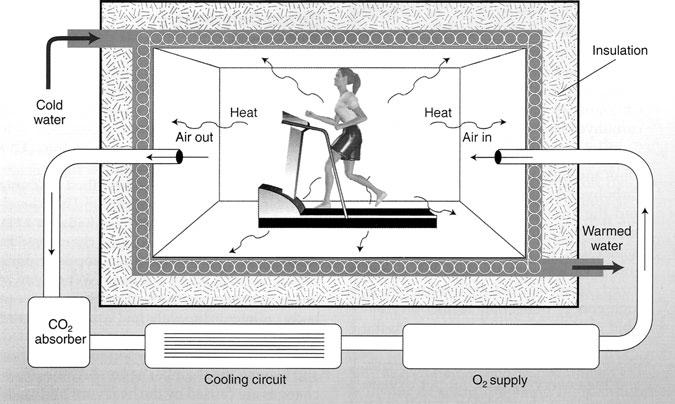
\includegraphics[width=0.8\textwidth]{66.png}
  \caption{En una cámara calorimétrica para calorimetría directa, el calor generado por la persona se transfiere al aire y a las paredes de la cámara, y el calor producido —y por lo tanto la tasa metabólica— se determinan mediante el cambio de temperatura medido en el aire y en el agua que fluye a través de la cámara.}
  \label{fig:66}
\end{figure}



La tasa metabólica durante el ejercicio se puede medir mediante calorimetría directa (Fig. 6.6) o calorimetría indirecta (Fig. 6.7). En la calorimetría directa (o de «bomba»), se mide el calor producido por una persona que realiza ejercicio en una habitación térmicamente aislada. La tasa metabólica se determina asumiendo que el $\sim 40\%$ de la energía liberada durante el metabolismo se utiliza para producir ATP, mientras que el $60\%$ restante se convierte en calor, el cual está siendo medido. El sujeto se encuentra en una cámara cerrada y térmicamente aislada. El calor producido por el cuerpo del sujeto calienta finalmente el agua que fluye por tuberías dentro de las paredes de la cámara, y se mide la temperatura de esta agua. Construir una cámara de este tipo es relativamente costoso y el tiempo de respuesta de este método es lento, por lo que las tasas metabólicas durante una actividad intensa no se pueden medir bien.

\begin{SCfigure}[1.0][htbp]
  \centering
  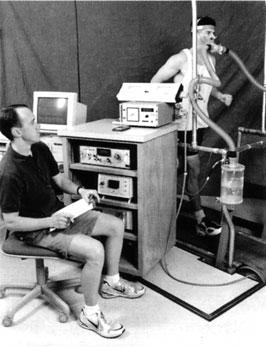
\includegraphics[width=0.45\textwidth]{67.png}
  \caption{Recolección de gases para la medición indirecta de las tasas metabólicas.}
  \label{fig:67}
\end{SCfigure}



En la calorimetría indirecta, se determinan las tasas de consumo de $\text{O}_2$, $d V_{\text{O}_2}/dt$, y producción de $\text{CO}_2$, $d V_{\text{CO}_2}/dt$, por lo que es más fácil de implementar, como se representa en la Fig. 6.7. Estas se determinan a partir de las tasas de volumen de aire inspirado y espirado, y de las fracciones de $\text{O}_2$ y $\text{CO}_2$ tanto en el aire inspirado como en el espirado (Problema 6.10). Si los equivalentes calóricos de los carbohidratos y las grasas fueran los mismos, la tasa de energía térmica producida sería $d V_{\text{O}_2}/dt \times$ el equivalente calórico. Debido a que no son los mismos, se mide la relación de intercambio respiratorio (RER) (Tabla 6.2) para determinar las cantidades relativas de carbohidratos y grasas que se están metabolizando. La RER se puede expresar como $(d V_{\text{CO}_2}/dt)/(d V_{\text{O}_2}/dt)$. Un valor de $\text{RER} = 1,0$ indica que los músculos están utilizando únicamente glucosa o glucógeno (carbohidratos). Un valor de $\text{RER} = 0,71$ indica que solo se están utilizando grasas. Los valores intermedios entre estos límites indican que se están utilizando tanto grasas como carbohidratos (Problema 6.10). Este enfoque supone que no se están metabolizando proteínas, lo cual no es cierto para el ejercicio que dura varias horas, durante el cual hasta el $10\%$ de la energía metabólica puede provenir del metabolismo de las proteínas.

Las capacidades aeróbicas de estudiantes universitarios normalmente activos de $18\text{--}22\text{ años}$ de edad son de $44\text{--}50\text{ mL/kg-min}$ (de oxígeno) para hombres y de $38\text{--}42\text{ mL/kg-min}$ para mujeres. Para atletas entrenados esta capacidad aumenta a unos $60\text{ mL/kg-min}$ y a $70\text{--}80\text{ mL/kg-min}$ o más para corredores masculinos de élite de larga distancia. Los adultos con un acondicionamiento físico deficiente pueden tener capacidades aeróbicas por debajo de $20\text{ mL/kg-min}$. La capacidad aeróbica disminuye con la edad, en aproximadamente un $10\%$ por década, comenzando a mediados de la adolescencia para las mujeres y a mediados de los 20 años para los hombres. Entre los hombres normalmente activos, esta disminuye desde aproximadamente $\sim 47,7\text{ mL/kg-min}$ a los $25\text{ años}$ de edad, a $\sim 43,1\text{ mL/kg-min}$ a los $35$, $\sim 39,5\text{ mL/kg-min}$ a los $45$, $\sim 38,4\text{ mL/kg-min}$ a los $52$, $\sim 34,5\text{ mL/kg-min}$ a los $63$, y $\sim 25,5\text{ mL/kg-min}$ a los $75\text{ años}$ de edad.

Todos estos cambios en las tasas metabólicas corporales están vinculados a los cambios correspondientes dentro de las células, órganos y sistemas del cuerpo. La Tabla 6.22 enumera la producción de potencia de diversas células y tejidos en diferentes niveles de actividad.

Al discutir las tasas metabólicas, debemos tener en cuenta que existen variaciones significativas en el metabolismo entre personas con las mismas características corporales y niveles de actividad. La variación habitual en la BMR es de $\pm 6\text{--}10\%$; presumiblemente, esto también es cierto para la TM (para los mismos niveles de actividad promedio). La Tabla 6.23 muestra un ejemplo sorprendente en el cual las tasas metabólicas de dos mujeres jóvenes difieren en un $50\%$. Debido a que la mayor parte de esta diferencia se debe al metabolismo durante el sueño por la noche, las posibles diferencias en los niveles de actividad no parecen muy importantes.

\begin{table}[htbp]
\centering
\caption{Producción de potencia estimada (tasas metabólicas) y densidades de potencia de células y tejidos biológicos (humanos, a menos que se indique lo contrario)}
\label{tab:622}
\small
\begin{tabularx}{\textwidth}{X >{\centering\arraybackslash}c >{\centering\arraybackslash}c >{\centering\arraybackslash}c}
\toprule
\textbf{Organelo, célula u objeto} & \textbf{Producción de potencia} & \textbf{Volumen} & \textbf{Densidad de potencia} \\
 & \textbf{(picovatios, pW)$^{\text{a}}$} & \textbf{($\mu\text{m}^3$)$^{\text{a}}$} & \textbf{($\text{W/m}^3$)} \\
\midrule
Puente cruzado de miosina & 0,000001 & $5 \times 10^{-7}$ & $2 \times 10^6$ \\
Plaqueta (en reposo) & 0,003\text{--}0,09 & 3 & $0,1\text{--}3,0 \times 10^4$ \\
Glóbulo rojo & 0,008 & 94 & $8,5 \times 10^1$ \\
Bacteria \textit{E. coli} (basal) & 0,05 & 2 & $2,5 \times 10^2$ \\
Organelo mitocondrial & 0,1\text{--}1,1 & 1 & $0,1\text{--}1,1 \times 10^6$ \\
Plaqueta (activada) & 0,7\text{--}7,0 & 3 & $0,2\text{--}2,3 \times 10^6$ \\
Célula de la piel & 1\text{--}3 & 1000 & $1,0\text{--}3,1 \times 10^3$ \\
Músculo esquelético (en reposo) & 1\text{--}10 & 2000 & $0,5\text{--}4,9 \times 10^3$ \\
Célula tisular típica (basal) & 30 & 8000 & $3,8 \times 10^3$ \\
Célula de intestino/estómago & 46\text{--}52 & 8000 & $5,6\text{--}6,5 \times 10^3$ \\
Neurona (basal) & 70\text{--}110 & 14\,000 & $5,0\text{--}7,9 \times 10^3$ \\
Célula muscular cardíaca (típica) & 87\text{--}290 & 8000 & $1,1\text{--}3,6 \times 10^4$ \\
Célula muscular esquelética (vol.) & 113 & 2000 & $5,7 \times 10^4$ \\
Célula renal & 155\text{--}346 & 8000 & $1,9\text{--}4,3 \times 10^4$ \\
Neurona (máxima) & 255\text{--}330 & 14\,000 & $1,8\text{--}2,4 \times 10^4$ \\
Célula tisular típica (máxima) & 480 & 8000 & $6,0 \times 10^4$ \\
Célula muscular esquelética (tet.) & 2300 & 2000 & $1,2 \times 10^6$ \\
Músculo de vuelo de abeja & 3400 & 1000 & $3,4 \times 10^6$ \\
Célula muscular cardíaca (máx.) & 3500\text{--}5000 & 8000 & $4,4\text{--}6,3 \times 10^5$ \\
Cerebro humano & $15\text{--}25\text{ W}$ & $1,4 \times 10^{-3}\text{ m}^3$ & $1,1\text{--}1,8 \times 10^4$ \\
Cuerpo humano (basal) & $100\text{ W}$ & $0,1\text{ m}^3$ & $1,0 \times 10^3$ \\
Cuerpo humano (máximo) & $1600\text{ W}$ & $0,1\text{ m}^3$ & $1,6 \times 10^4$ \\
Automóvil de gasolina & $200\,000\text{ W}$ & $10\text{ m}^3$ & $2,0 \times 10^4$ \\
El Sol & $3,92 \times 10^{26}\text{ W}$ & $1,41 \times 10^{27}\text{ m}^3$ & 0,28 \\
\bottomrule
\end{tabularx}
\begin{flushleft}
    \small $^{\text{a}}$ A menos que se indique otra unidad.\\
    Nota: tenga en cuenta que $1\text{ W} = 0,86\text{ kcal/h}$.\\
    Utilizando datos presentados en \cite{38}.
\end{flushleft}
\end{table}

\begin{table}[htbp]
\centering
\caption{Ingesta de alimentos y producción de calor para dos mujeres de $23\text{ años}$ de tamaño físico comparable}
\label{tab:623}
\small
\begin{tabularx}{0.8\textwidth}{Xccc}
\toprule
 & \textbf{«Gran comedora»} & \textbf{«Pequeña comedora»} & \textbf{Relación} \\
\midrule
Masa corporal (kg) & 54,2 & 52,7 & 1,03 \\
Masa corporal magra (kg) & 45,1 & 43,6 & 1,03 \\
Ingesta promedio de alimentos (kcal/día) & 2370 & 1550 & 1,54 \\
Producción de calor (kcal/día) & 2170 & 1390 & 1,55 \\
Producción de calor por la noche (kcal/día) & 1720 & 1100 & 1,56 \\
\bottomrule
\end{tabularx}
\begin{flushleft}
    \small Utilizando datos de \cite{11}, a partir del resultado de Warwick citado por \cite{39}.
\end{flushleft}
\end{table}

\begin{SCfigure}[0.9][htbp]
  \centering
  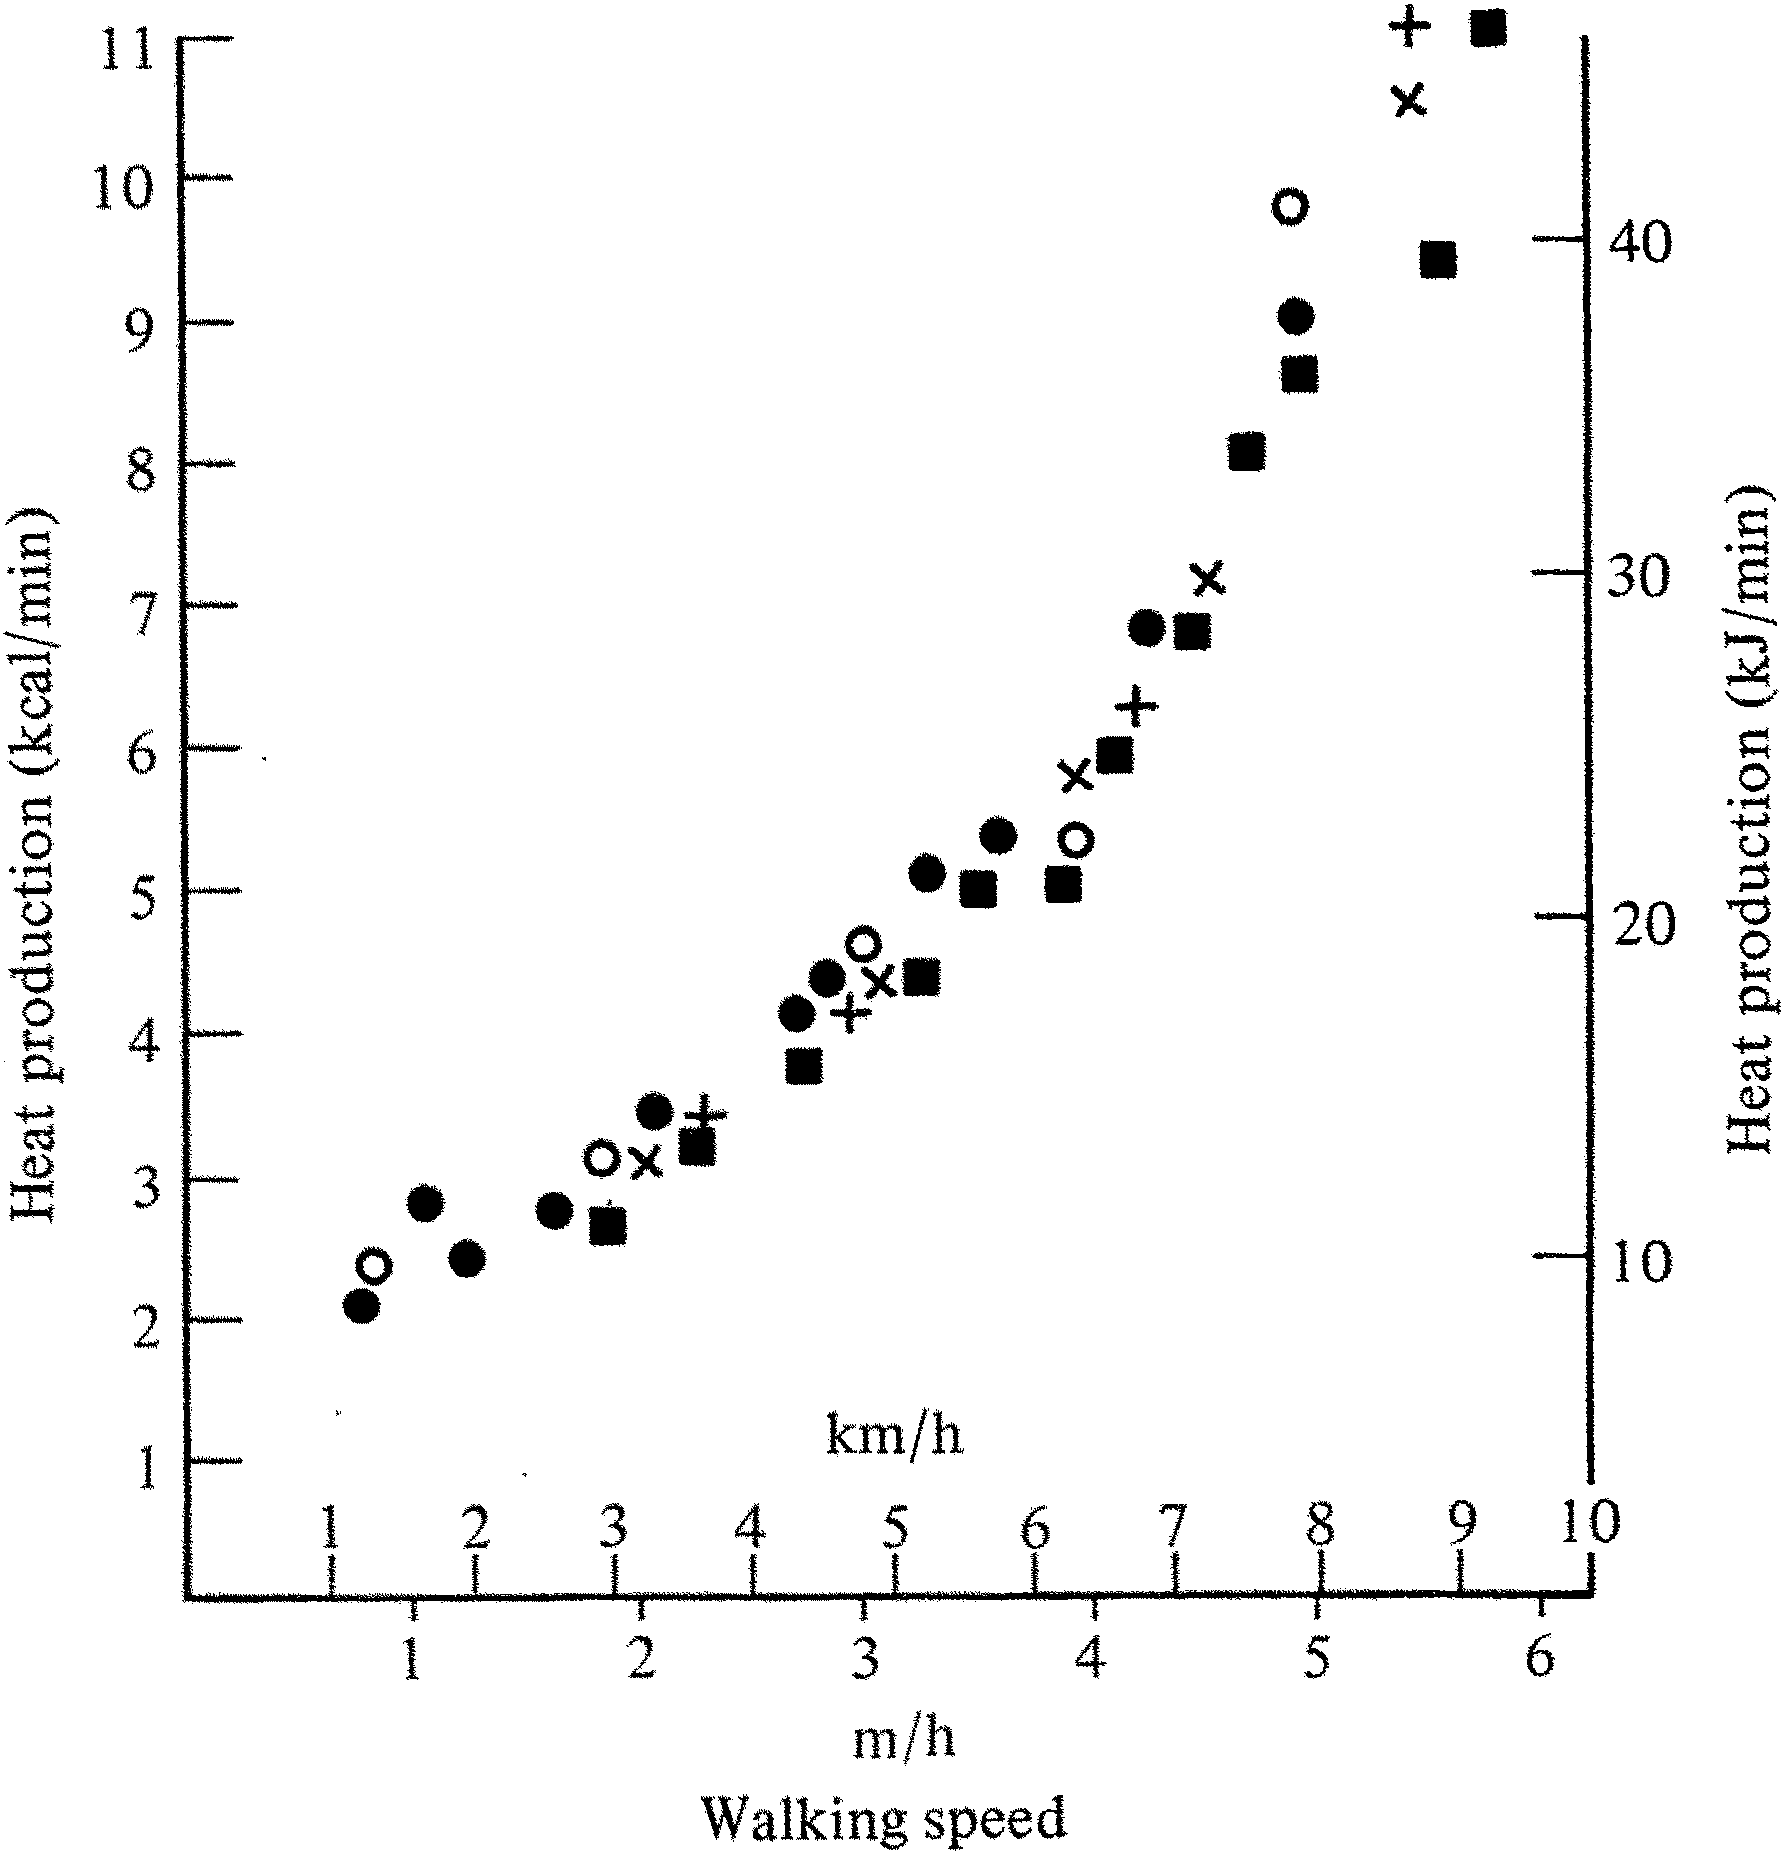
\includegraphics[width=0.5\textwidth]{68.png}
  \caption{Producción de calor (necesidades metabólicas) de la marcha.}
  \label{fig:68}
\end{SCfigure}



\subsubsection*{Tasas metabólicas durante la locomoción}

La Figura 6.8 muestra que la tasa de producción de calor en función de la velocidad de marcha es aproximadamente lineal, lo que significa que el costo de energía por distancia recorrida es independiente de la velocidad. Por encima de $3\text{ m/s}$ ($7\text{ mph}$), esta curva se vuelve muy superlineal. El costo energético de caminar por encima del de estar de pie es de $\sim 2,13\text{ J/kg-m}$ a $1,2\text{ m/s}$ ($2,6\text{ mph}$), $\sim 2,49\text{ J/kg-m}$ a $1,8\text{ m/s}$ ($4,0\text{ mph}$) y $\sim 3,93\text{ J/kg-m}$ a $2,4\text{ m/s}$ ($5,4\text{ mph}$).

\begin{SCfigure}[0.8][htbp]
  \centering
  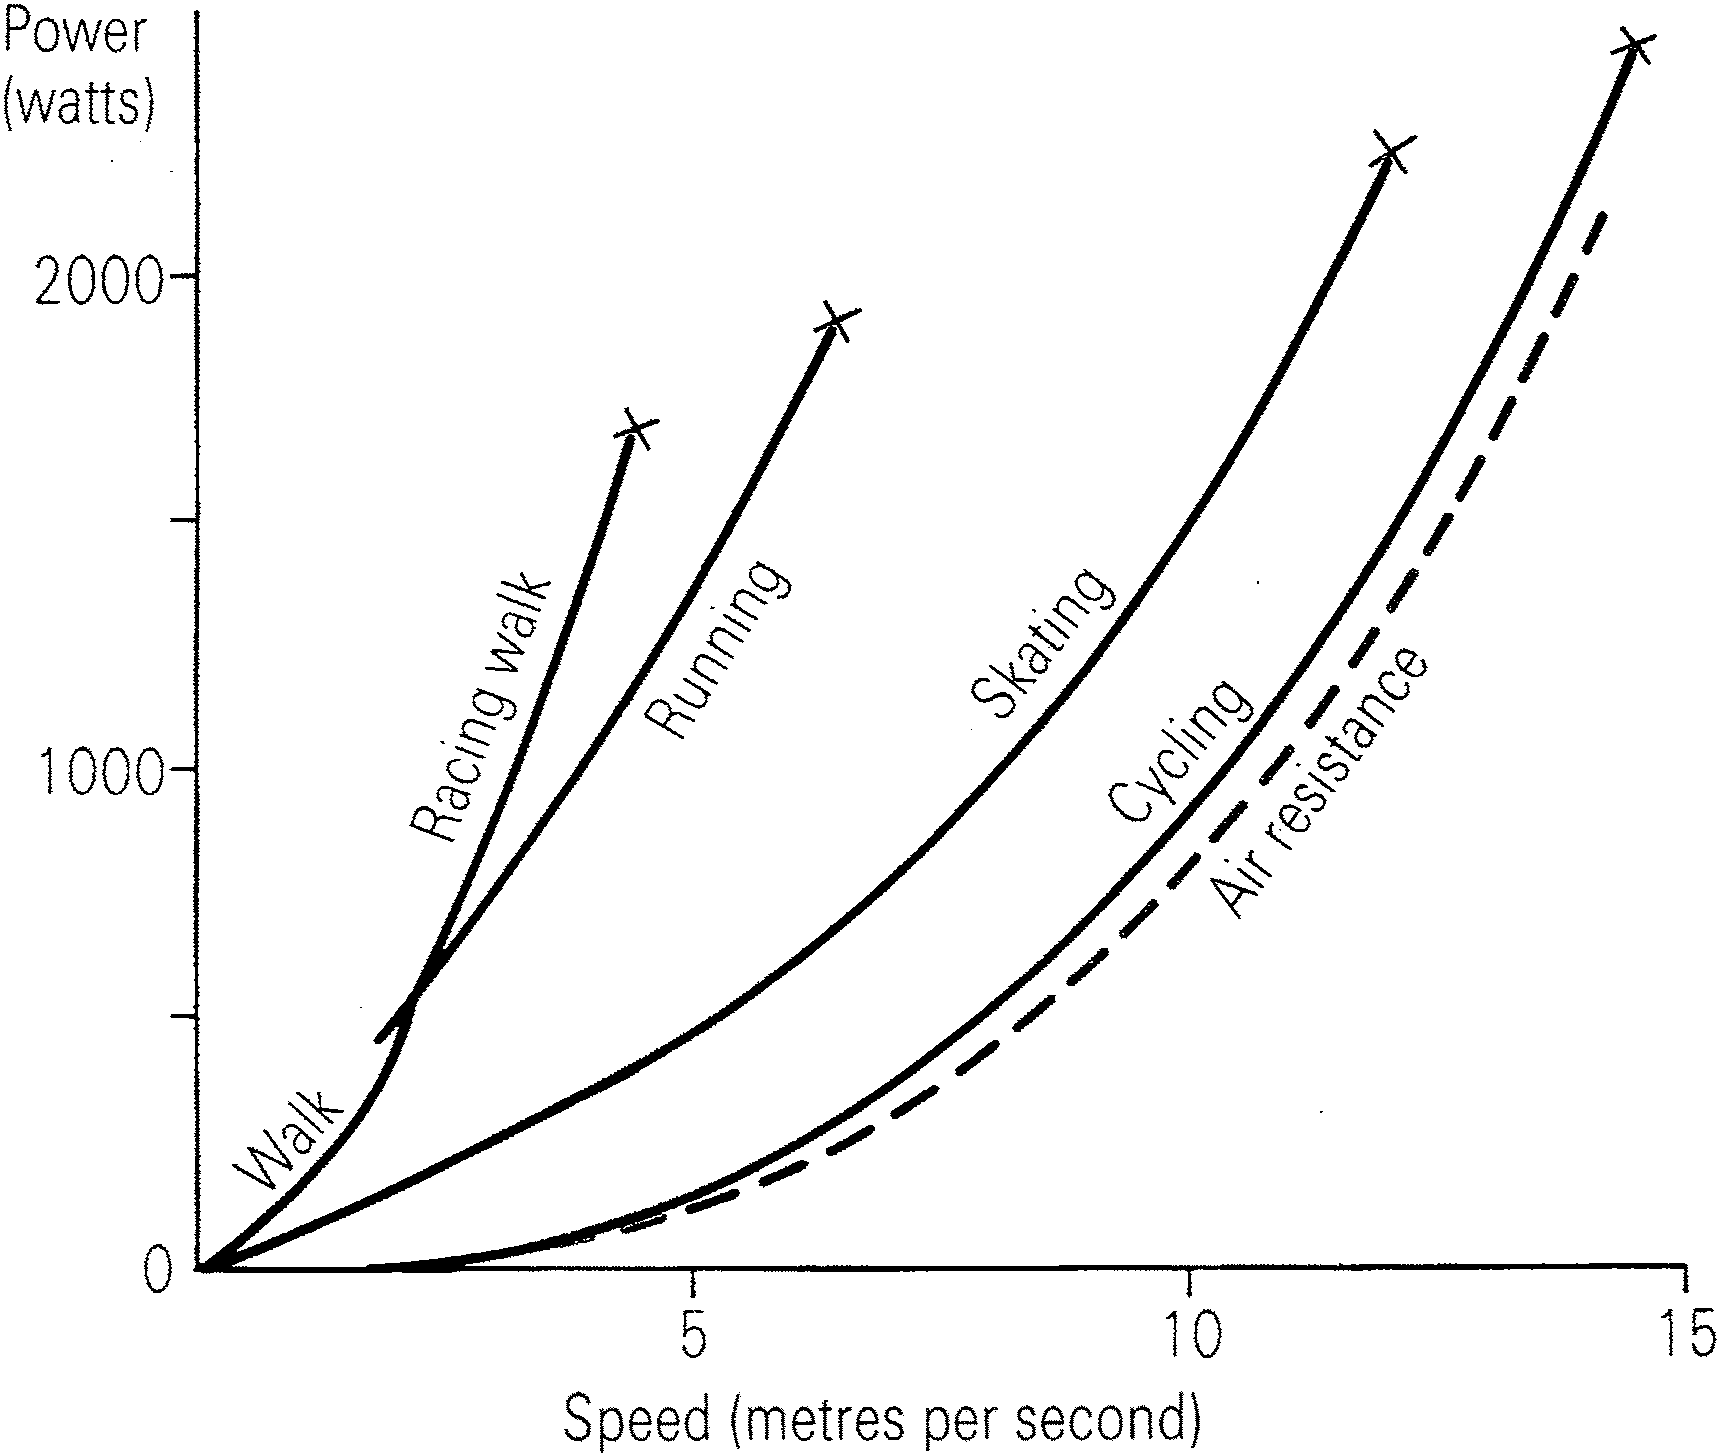
\includegraphics[width=0.55\textwidth]{69.png}
  \caption{Necesidades metabólicas frente a la velocidad para varios tipos de locomoción, extrapoladas a las velocidades de récord mundial para carreras de $5\text{ km}$ (para correr) o carreras de $10\text{ km}$ (para los demás). La línea discontinua muestra la potencia necesaria para superar únicamente la resistencia del aire.}
  \label{fig:69}
\end{SCfigure}



A altas velocidades, ¿por qué preferimos correr a caminar? Es muy difícil seguir caminando a estas velocidades más rápidas debido a la mayor potencia necesaria en relación con el trote y la carrera (Fig. 3.26). De hecho, a $2,4\text{ m/s}$ ($5,4\text{ mph}$), la potencia metabólica necesaria para correr es un $14\%$ menor que la necesaria para caminar. Expresado en términos de la energía necesaria por unidad de masa para moverse horizontalmente por metro, esto representa una disminución de $\sim 3,93\text{ J/kg-m}$ ($0,94\text{ cal/kg-m}$) a $\sim 3,40\text{ J/kg-m}$ ($0,81\text{ cal/kg-m}$). La Figura 3.26 muestra que el costo metabólico de la locomoción por distancia recorrida es relativamente independiente de la velocidad para una amplia gama de velocidades cuando se utiliza la marcha óptima, tanto para humanos como para caballos. La energía necesaria para correr en terreno plano es de $\sim 4,2\text{ J/kg-m}$ para corredores no entrenados, independiente de la velocidad, lo cual es aproximadamente el doble que para caminar a la velocidad de marcha más económica desde el punto de vista energético, de $4\text{ km/h}$. Esta energía es un $\sim 6\%$ menor que este valor para corredores entrenados \cite{60}. (Aunque cuesta la misma energía caminar una milla rápidamente que correr una milla, correr proporciona un mejor entrenamiento cardiovascular). La ingesta de oxígeno es de aproximadamente $5,8\text{ mL/kg-min}$ por cada mph de velocidad de carrera. La Figura 6.9 muestra las necesidades metabólicas frente a la velocidad para varios tipos de locomoción.

Se dice que las contracciones musculares concéntricas realizan trabajo positivo, mientras que las contracciones excéntricas realizan trabajo negativo (véase la Fig. 3.56). El costo metabólico del trabajo positivo es mayor que una cantidad igual de trabajo negativo. La energía adicional promedio necesaria para moverse horizontalmente, de $\sim 2,8\text{ J/kg-m}$ (en relación con estar de pie), es mucho menor que la adicional necesaria para moverse verticalmente, de $\sim 30\text{ J/kg-m}$. Obviamente, caminar cuesta arriba requiere más potencia que en terreno plano; caminar cuesta abajo requiere menos potencia que en terreno plano. El trabajo y la potencia requeridos para subir una cuesta son aproximadamente $2,7 \times$ el aumento en la energía potencial y la tasa concomitante de cambio de esta energía; esto significa que la eficiencia para realizar este tipo de trabajo es de aproximadamente $1/2,7 = 36\%$. (Como veremos pronto, esto indica que la energía adicional promedio necesaria para moverse verticalmente es de $26\text{ J/kg-m}$, lo cual es consistente con el valor de $\sim 30\text{ J/kg-m}$ que se acaba de dar). Al moverse cuesta abajo, se necesita menos potencia que en terreno plano en un $\sim 50\%$ de la tasa de disminución de la energía potencial. Toda la energía potencial ganada no se recupera porque se requiere trabajo muscular para evitar que caigamos cuesta abajo. El Problema 6.65 explora la potencia necesaria al caminar (o correr) y las pendientes.

\begin{table}[htbp]
\centering
\caption{El protocolo de Bruce para una prueba de esfuerzo en una caminadora}
\label{tab:624}
\small
\begin{tabularx}{0.8\textwidth}{Xccc}
\toprule
\textbf{Etapa} & \textbf{Velocidad (mph)} & \textbf{Pendiente (\%)} & \textbf{Tiempo acumulado (min)} \\
\midrule
I & 1,7 & 10 & 1\text{--}3 \\
II & 2,5 & 12 & 4\text{--}6 \\
III & 3,4 & 14 & 7\text{--}9 \\
IV & 4,2 & 16 & 10\text{--}12 \\
V & 5,0 & 18 & 13\text{--}15 \\
\bottomrule
\end{tabularx}
\begin{flushleft}
    \small Utilizando datos de \cite{35}.
\end{flushleft}
\end{table}

Abordemos el uso de las caminadoras para evaluar la capacidad cardiovascular y cardiorrespiratoria de personas sanas y de aquellas con enfermedades cardíacas. El paciente se conecta con cables de ECG (electrocardiograma) y se toman lecturas continuas de ECG mientras el paciente camina o corre en la caminadora (véanse los Caps. 8 y 12 para más información sobre los ECG). La velocidad de la caminadora y/o la pendiente cuesta arriba se incrementan después de períodos de tiempo establecidos (llamados etapas), hasta que el ciclo completo termina, el paciente ya no puede tolerar el esfuerzo o aparece alguna irregularidad. En el Protocolo de Bruce (Tabla 6.24), la velocidad y la pendiente aumentan en cada etapa. En otro protocolo común, el Protocolo de Naughton, la velocidad se fija en $3,0\text{ mph}$ y la pendiente aumenta desde el $2,5\%$ en la Etapa I hasta el $20,0\%$ en la Etapa VIII, en incrementos de $2,5\%$, durando cada etapa $2\text{ min}$. Dichas caminadoras inclinables también se utilizan para determinar la eficiencia de los músculos esqueléticos en la locomoción humana. Las tasas de consumo de oxígeno —y, por lo tanto, las tasas metabólicas— se comparan para un grupo de personas que se mueven a una velocidad dada, primero en una caminadora nivelada y luego en una caminadora inclinada. La eficiencia es de aproximadamente el $30\%$.

Como ejemplo, determinaremos la potencia metabólica y la tasa de consumo de oxígeno necesarias durante la Etapa V del protocolo de Bruce para un varón de $75\text{ kg}$. La tasa total es la suma de la BMR (o más precisamente la TM al estar de pie), la potencia necesaria para moverse horizontalmente y la potencia adicional necesaria para moverse cuesta arriba. El segundo término es $\sim 2,8\text{ J/kg-m} \times$ (distancia horizontal recorrida por unidad de tiempo). Esto es $2,8\text{ W } m_{\text{b}} v$, donde $m_{\text{b}}$ es la masa corporal en $\text{kg}$ y $v$ es la velocidad de marcha en $\text{m/s}$ (o más bien trote a esta velocidad más rápida). El tercer término proviene de la rapidez con la que cambia la energía potencial $m_{\text{b}}gh$ con el tiempo, que es $m_{\text{b}}g(dh/dt)$, y el factor de «ineficiencia» de $2,7$, por lo que es $2,7 m_{\text{b}}g(dh/dt)$. Una persona que se mueve una distancia $x$ a lo largo de una rampa a un ángulo $\theta$ se eleva una distancia $x \sin \theta$ (dibuje un diagrama para demostrarlo), por lo que este tercer término se convierte en $2,7 m_{\text{b}}g \sin \theta (dx/dt)$. Con $v = dx/dt$, esto se convierte en $2,7 m_{\text{b}}gv \sin \theta = 26\text{ W } m_{\text{b}}v \sin \theta$. La combinación del segundo y tercer término da $(2,8 + 26 \sin \theta) m_{\text{b}}v$ en $\text{W}$ o $(2,4 + 22,8 \sin \theta) m_{\text{b}}v$ en $\text{kcal/h}$ (utilizando $1\text{ W} = 0,86\text{ kcal/h}$). La velocidad es de $5,0\text{ mph} = 2,23\text{ m/s}$ (utilizando $1\text{ mph} = 0,447\text{ m/s}$). Una pendiente del $18\%$ corresponde a un ángulo de $(0,18)90^\circ = 16,2^\circ$, por lo que $\sin \theta = 0,28$. Para esta persona de $75\text{ kg}$, el segundo término es $(2,4)(75)(2,23) = 401\text{ kcal/h}$ y el tercer término es $(22,8)(0,28)(75)(2,23) = 1068\text{ kcal/h}$. La carga de moverse cuesta arriba rápidamente es con diferencia la mayor contribución a la tasa metabólica. La suma de estos dos términos es $1469\text{ kcal/h}$. Sumando a esto la TM al estar de pie de aproximadamente $100\text{ kcal/h}$, la TM en la Etapa V es de aproximadamente $1570\text{ kcal/h}$, lo cual es bastante alto. (Por supuesto, el paciente se encuentra en esta etapa no más de $3\text{ min}$). Asumiendo únicamente metabolismo aeróbico, la tasa de uso de oxígeno es esta tasa metabólica dividida por el equivalente calórico. Si solo se están quemando carbohidratos, el equivalente calórico es de $5,05\text{ kcal/L de O}_2$ y vemos que en la Etapa V se necesita $d V_{\text{O}_2}/dt = (1570\text{ kcal/h}) / (5,05\text{ kcal/L de O}_2) = 311\text{ L de O}_2\text{/h} = 5,2\text{ L de O}_2\text{/min}$.

\begin{table}[htbp]
\centering
\caption{El efecto del viento en las necesidades energéticas de caminar y correr}
\label{tab:625}
\small
\begin{tabularx}{\textwidth}{X >{\centering\arraybackslash}c >{\centering\arraybackslash}c >{\centering\arraybackslash}c >{\centering\arraybackslash}c}
\toprule
\textbf{Actividad, velocidad} & \textbf{Velocidad del viento $w$} & \textbf{Consumo de} & \textbf{Producción} & \textbf{Incremento en} \\
\textbf{(m/s) (o mph)} & \textbf{(m/s) (o mph)} & \textbf{oxígeno (L/min)} & \textbf{de calor (W)} & \textbf{la energía/$w^2$ ($\text{W-s}^2\text{/m}^2$)} \\
\midrule
Caminar, 1,25 (2,80) & 0,0 (0,0) & 0,878 & 294 & -- \\
 & 10,0 (22,4) & 1,192 & 399 & $\simeq 1,05$ \\
 & 14,1 (31,5) & 1,505 & 504 & $\simeq 1,05$ \\
\midrule
Caminar, 2,08 (4,65) & 0,0 (0,0) & 1,649 & 552 & -- \\
 & 10,0 (22,4) & 2,221 & 744 & $\simeq 1,91$ \\
 & 14,1 (31,5) & 2,792 & 935 & $\simeq 1,91$ \\
\midrule
Correr, 3,75 (8,39) & 0,0 (0,0) & 2,836 & 950 & -- \\
 & 10,0 (22,4) & 3,243 & 1086 & $\simeq 1,36$ \\
 & 14,1 (31,5) & 3,710 & 1243 & $\simeq 1,36$ \\
\midrule
Correr, 4,47 (10,00) & 0,0 (0,0) & 3,010 & 1008 & -- \\
 & 10,0 (22,4) & 3,710 & 1243 & $\simeq 2,52$ \\
 & 14,1 (31,5) & 4,525 & 1516 & $\simeq 2,52$ \\
\bottomrule
\end{tabularx}
\begin{flushleft}
    \small Nota: la última columna es el incremento en la producción de calor dividido por el cuadrado de la velocidad del viento para las condiciones particulares de caminata o carrera.\\
    Utilizando datos de \cite{11}, calculados a partir de \cite{86}.
\end{flushleft}
\end{table}

¿Por qué es difícil correr contra el viento? La respuesta es que requiere mucha más potencia metabólica (producción de calor o consumo equivalente de oxígeno). La Tabla 6.25 muestra que para caminar y correr esta potencia aumenta como el cuadrado de la velocidad del viento. Una caminata rápida contra el viento puede requerir tanta potencia como una carrera relativamente lenta sin viento. Incluso el aire en calma afecta las necesidades metabólicas; la resistencia del aire representa aproximadamente el $8\%$ de las necesidades metabólicas para los corredores de media distancia y hasta el $15\%$ para los velocistas. (Examinamos este efecto de la resistencia aerodinámica en el Cap. 7).

\subsubsection*{Escalamiento de la TM con equivalentes metabólicos y factores de actividad}

La producción real de calor, o tasa metabólica (TM), es mayor que la BMR debido a la actividad (Tabla 6.21). Podemos relacionar la TM y la BMR mediante
\begin{equation}
\text{TM} = f (\text{BMR}),
\label{eq:632}
\end{equation}
donde $f$ es el factor de actividad.

El equivalente metabólico (MET) es otra medida de actividad muy estrechamente relacionada. Un cuerpo promedio consume ($3,5\text{ mL/kg-min}$) $\times \text{MET}$. Los valores típicos de MET se presentan en las Tablas 6.26, 6.27, 6.28, 6.29 y 6.30. A menudo se dice que $\text{MET} \sim f/1,5$, debido a que el factor de actividad $f$ se toma con referencia a la BMR, que es menor, pero no es probable que esta relación sea tan grande como $1,5$, especialmente para actividades ligeras. (Al comparar los valores para caminar con los de \cite{47}, esta relación parece estar más cerca de $1,2$ para actividades moderadas). Los ejemplos de $f$ \cite{47} incluyen $1,05$ para estar acostado en reposo, $1,20$ para tejer, $1,48$ para jugar a las cartas, $2,36$ para trabajar en una línea de montaje de automóviles, $3,02$ para jugar al billar, $3,66$ para sacudir el polvo, $4,22$ para bailar el vals, $5,03$ para deshierbar y $5,08$ para competencias de marcha militar.

\begin{table}[htbp]
\centering
\caption{Valores típicos de MET para el cuidado personal}
\label{tab:626}
\small
\begin{tabularx}{0.8\textwidth}{X >{\centering\arraybackslash}c}
\toprule
\textbf{Cuidado personal} & \textbf{MET} \\
\midrule
Descanso, estar sentado, de pie, comer, conversar & 1,0 \\
Vestirse, desvestirse, lavarse las manos y la cara, propulsar silla de ruedas & 2,0 \\
Caminar a $2,5\text{ mph}$ & 3,0 \\
Ducharse & 3,5 \\
Bajar escaleras & 4,5 \\
Caminar a $3,5\text{ mph}$ & 5,5 \\
\bottomrule
\end{tabularx}
\begin{flushleft}
    \small Utilizando datos de \cite{106}.
\end{flushleft}
\end{table}

\begin{table}[htbp]
\centering
\caption{Valores típicos de MET para el trabajo doméstico}
\label{tab:627}
\small
\begin{tabularx}{0.8\textwidth}{X >{\centering\arraybackslash}c}
\toprule
\textbf{Trabajo doméstico} & \textbf{MET} \\
\midrule
Coser a mano & 1,0 \\
Coser a máquina, barrer el suelo & 1,5 \\
Lustrar muebles & 2,0 \\
Pelar patatas, fregar, lavar ropa a mano, amasar masa & 2,5 \\
Fregar suelos, limpiar ventanas, hacer camas & 3,0 \\
Planchar, trapear, escurrir ropa a mano, colgar ropa a mano & 3,5 \\
Sacudir alfombras & 4,0 \\
\bottomrule
\end{tabularx}
\begin{flushleft}
    \small Utilizando datos de \cite{106}.
\end{flushleft}
\end{table}

Como se señaló anteriormente, existe una aparente inconsistencia en nuestra discusión de la BMR, la TM y los factores de actividad. Entre los humanos, la BMR varía de manera más lenta que lineal con $m_{\text{b}}$, de una forma que es aproximadamente, pero no exactamente, la misma que la dependencia de $m_{\text{b}}^{3/4}$ de la Ley de Kleiber. Adoptar el factor de actividad (o PAR) como la relación entre la TM y la BMR para una actividad dada presume que la tasa metabólica adicional debido a esa actividad también varía aproximadamente como $m_{\text{b}}^{3/4}$; sin embargo, la tasa metabólica adicional debido a la locomoción es proporcional a $m_{\text{b}}$. Aún no se comprende bien cómo depende de la masa corporal la energía que gastamos en diferentes actividades.

\begin{table}[htbp]
\centering
\caption{Valores típicos de MET para ocupaciones}
\label{tab:628}
\small
\begin{tabularx}{0.8\textwidth}{X >{\centering\arraybackslash}c}
\toprule
\textbf{Ocupación} & \textbf{MET} \\
\midrule
Sentado en escritorio, escribir, andar en auto, reparación de relojes & 1,5 \\
Escribir en computadora & 2,0 \\
Soldadura, montaje de radios, tocar instrumento musical & 2,5 \\
Montaje de piezas & 3,0 \\
Albañilería, enyesado & 3,5 \\
Trabajo de montaje pesado, empujar carretilla ($115\text{ lb}$, $2,5\text{ mph}$) & 4,0 \\
Carpintería & 5,5 \\
Cortar el césped con cortadora manual, picar leña & 6,5 \\
Palear & 7,0 \\
Cavar & 7,5 \\
\bottomrule
\end{tabularx}
\begin{flushleft}
    \small Utilizando datos de \cite{106}.
\end{flushleft}
\end{table}

\begin{table}[htbp]
\centering
\caption{Valores típicos de MET para ejercicio}
\label{tab:629}
\small
\begin{tabularx}{0.8\textwidth}{X >{\centering\arraybackslash}c}
\toprule
\textbf{Ejercicio (condiciones niveladas)} & \textbf{MET} \\
\midrule
Caminar a $2\text{ mph}$ & 2,5 \\
Ciclismo a $5,5\text{ mph}$ & 3,0 \\
Caminar a $2,5\text{ mph}$, ciclismo a $6\text{ mph}$ & 3,5 \\
Caminar a $3\text{ mph}$; calistenia & 4,5 \\
Ciclismo a $9,7\text{ mph}$; natación, crol, a $1,0\text{ ft/s}$ & 5,0 \\
Caminar a $3,5\text{ mph}$ & 5,5 \\
Caminar a $4\text{ mph}$ & 6,5 \\
Trotar a $5\text{ mph}$ & 7,5 \\
Correr a $7,5\text{ mph}$; ciclismo a $13\text{ mph}$ & 9,0 \\
Natación, crol, a $2,0\text{ ft/s}$ & 10,0 \\
Correr a $8,5\text{ mph}$ & 12,0 \\
Correr a $10\text{ mph}$; natación, crol, a $2,5\text{ ft/s}$ & 15,0 \\
Correr a $12\text{ mph}$; natación, crol, a $3,0\text{ ft/s}$ & 20,0 \\
Correr a $15\text{ mph}$; natación, crol, a $3,5\text{ ft/s}$ & 30,0 \\
\bottomrule
\end{tabularx}
\begin{flushleft}
    \small Utilizando datos de \cite{106}.
\end{flushleft}
\end{table}

\subsubsection*{Factor de actividad promedio diario}

El factor de actividad podría referirse a una actividad dada, como se indicó anteriormente, o al promedio diario, al cual llamaremos $f_{\text{av}}$. (El término nivel de actividad física (PAL, por sus siglas en inglés) se utiliza comúnmente en la comunidad de la salud). No existe un acuerdo universal sobre los valores reales de $f_{\text{av}}$. Estos dependen del tipo de trabajo, la cantidad de ejercicio y el acceso a comodidades automatizadas. Estudios de las Naciones Unidas sugieren para hombres adultos un $f_{\text{av}} \sim 1,55$ para trabajo ocupacional ligero, $1,78$ para trabajo ocupacional moderado y $2,10$ para trabajo ocupacional pesado. Esto es consistente con otra evaluación, presentada de manera diferente, que estima que es de aproximadamente $1,2$ para aquellos en reposo absoluto en cama, $\sim 1,6$ para oficinistas sedentarios, $\sim 1,8$ para quienes se dedican a la manufactura o la agricultura, $\sim 2$ para agricultores de subsistencia y «cazadores-recolectores» modernos (que cazan y recolectan alimentos, como en la tribu Hadza en Tanzania) \cite{7} y $\sim 2,5$ durante el entrenamiento para eventos de resistencia, como el maratón \cite{56}. También se han sugerido valores «deseables» de $f_{\text{av}}$ de $\sim 1,65$ para adolescentes y adultos hasta los $59\text{ años}$ de edad en países desarrollados (y $\sim 1,8$ en países en desarrollo) y de $\sim 1,5$ para aquellos de $60\text{ años}$ o más \cite{33,47}. Otros estudios sugieren que la TM es mucho menor, con un $f_{\text{av}} \sim 1,3$ para actividad baja (sedentaria), $\sim 1,5$ para actividad intermedia (algo de ejercicio regular) y $\sim 1,7$ para una actividad de alto nivel (actividad regular o trabajo físicamente exigente). Para una dieta de supervivencia que incluya la energía necesaria para comer y digerir los alimentos y la higiene esencial, pero no la necesaria para ganarse la vida o preparar los alimentos, se ha estimado que el $f_{\text{av}}$ es de $1,27$ \cite{34}.

\begin{table}[htbp]
\centering
\caption{Valores típicos de MET para recreación}
\label{tab:630}
\small
\begin{tabularx}{0.8\textwidth}{X >{\centering\arraybackslash}c}
\toprule
\textbf{Actividad recreativa} & \textbf{MET} \\
\midrule
Pintar, sentado & 1,5 \\
Tocar el piano, conducir un auto & 2,0 \\
Hacer canotaje a $2,5\text{ mph}$, montar a caballo (al paso) & 2,5 \\
Voleibol (recreativo), billar & 3,0 \\
Bolos, juego de herraduras & 3,5 \\
Golf, críquet & 4,0 \\
Tiro con arco, baile de salón, ping-pong (tenis de mesa), béisbol & 4,5 \\
Tenis & 6,0 \\
Montar a caballo (al trote), danza folclórica & 6,5 \\
Esquí, montar a caballo (al galope) & 8,0 \\
Squash & 8,5 \\
Esgrima, baloncesto, fútbol americano & 9,0 \\
Gimnasia, balonmano, paleta & 10,0 \\
\bottomrule
\end{tabularx}
\begin{flushleft}
    \small Utilizando datos de \cite{106}.
\end{flushleft}
\end{table}

El más alto de estos valores para el trabajo ocupacional pesado, $f_{\text{av}} \sim 2,10$, es aún menor que el estimado para un minero de carbón escocés en la década de 1950, antes de que la ocupación se automatizara más. La tasa metabólica máxima del minero de carbón era de $4,3 \times \text{BMR}$ durante las horas de trabajo y promediaba un valor aún muy alto de $2,5 \times \text{BMR}$ durante todo el día, como se calcula en la Tabla 6.31. La mayoría de las ocupaciones son físicamente menos exigentes ahora y, en general, los estilos de vida modernos requieren mucha menos actividad física. El trabajo doméstico es mucho menos exigente físicamente con el uso generalizado de lavadoras de ropa, aspiradoras, lavavajillas y procesadores de alimentos. El tiempo dedicado a las tareas del hogar cada semana ha disminuido aproximadamente a la mitad en los últimos $50\text{ años}$ \cite{5}.

Los estadounidenses típicos caminan $\sim 1/4$~de milla al día y los europeos occidentales $\sim 2/3$~de milla al día, mucho menos que las $\sim 5\text{--}9$~millas al día de los cazadores-recolectores modernos \cite{7}. Los cazadores-recolectores masculinos tienen una masa corporal de $\sim 51\text{ kg}$, caminan alrededor de $9\text{ millas}$ cada día y tienen una $f_{\text{av}} \sim 2650\text{ kcal/día} \text{ (TM)} / 1170\text{ kcal/día} \text{ (BMR)} = 2,26$, lo cual supera a la de los varones occidentales de $\sim 81\text{ kg}$, $3050\text{ kcal/día} / 1685\text{ kcal/día} = 1,81$. Estos cazadores-recolectores utilizan aproximadamente el doble de kcal por kg de masa corporal en las actividades, $(2650 - 1170)/51 = 29{,}0\text{ kcal/kg}$, en comparación con los occidentales típicos, $(3050 - 1685)/81 = 16{,}9\text{ kcal/kg}$. No es sorprendente que también tengan un IMC menor, $\sim 20{,}3$ frente a $\sim 25{,}6\text{ kg/m}^2$, y menos grasa corporal, $\sim 13{,}5\%$ frente a $\sim 22{,}5\%$ \cite{56,62,82}.

Aun así, las tasas metabólicas (TM) humanas sostenidas no suelen superar $2{,}0\text{--}2{,}5 \times \text{BMR}$, excepto para aquellos en ocupaciones de alto rendimiento, como los atletas de resistencia. Esto podría constituir un techo metabólico para los seres humanos \cite{29,46,78}. Este límite es superado por los ciclistas del Tour de Francia, quienes tienen un factor de actividad promedio de $\sim 4{,}3$, pero no por los cazadores-recolectores.

¿Por qué las mujeres normalmente dan a luz entre $38\text{ y }40\text{ semanas}$ después de la concepción? La razón parece relacionarse con el tamaño fetal en ese momento. Algunos piensan que está limitado por los tamaños de la cadera y del canal de parto en relación con el tamaño de la cabeza fetal (la cual es grande a pesar de que el tamaño del cerebro al nacer es solo el $30\%$ del tamaño final). Si los tamaños de las caderas fueran mayores, tal vez la locomoción en las mujeres requeriría más energía (y esto no sería deseable), pero hay evidencia de que este no es el caso \cite{29}. El final del embarazo podría estar indicado por un cruce entre las tasas metabólicas de la madre y las necesidades metabólicas fetales \cite{29,30}. Existe cierta indicación de que la TM total de una mujer embarazada se estabiliza en aproximadamente $2{,}1$ veces su BMR previa al embarazo en algún momento durante la segunda mitad de la gestación, lo cual sería consistente con un techo de TM de $2{,}0\text{--}2{,}5 \times \text{BMR}$ \cite{29,46,78}. Si esto fuera realmente un límite, la madre podría no ser capaz de sostener una ingesta calórica suficiente para satisfacer las necesidades calóricas de rápido crecimiento al final del embarazo, cuando el feto comienza a crecer muy rápido. Si este cruce ocurre $\simeq 40\text{ semanas}$ después de la gestación, esta podría ser la razón por la cual las señales hormonales que conducen al parto ocurren en ese momento y no más tarde. (Las crecientes necesidades metabólicas del feto pueden apreciarse al observar que los requerimientos metabólicos para los lactantes aumentan de $450\text{ a }1000\text{ kcal/día}$ desde el nacimiento hasta los $12\text{ meses}$ \cite{33}. Esto incluye las necesidades calóricas para soportar el tejido en crecimiento en el bebé, pero también incluye las necesidades metabólicas que respaldan el movimiento del bebé y la función de sus órganos que no ocurrirían en un feto, y excluye otras necesidades metabólicas de la madre durante el embarazo).

\begin{table}[htbp]
\centering
\caption{Análisis de las necesidades de potencia metabólica de un minero de carbón escocés a principios de la década de 1950, antes de la mecanización}
\label{tab:631}
\small
\begin{tabularx}{\textwidth}{X >{\centering\arraybackslash}c >{\centering\arraybackslash}c >{\centering\arraybackslash}c >{\centering\arraybackslash}c}
\toprule
\textbf{Actividad} & \textbf{Tiempo} & \textbf{Fracción del} & \textbf{TM/BMR} & \textbf{Producto} \\
 & \textbf{(min)} & \textbf{día, $F$} & \textbf{$= f$} & \textbf{$F \times f$} \\
\midrule
En cama & 501 & 0,348 & 1,00 & 0,348 \\
\midrule
\multicolumn{5}{l}{\textit{No ocupacional}} \\
Sentado & 331 & 0,230 & 1,51 & 0,347 \\
De pie & 19 & 0,013 & 1,71 & 0,022 \\
Caminando & 129 & 0,089 & 4,67 & 0,416 \\
Aseándose y vistiéndose & 43 & 0,030 & 3,14 & 0,094 \\
Jardinería & 17 & 0,012 & 4,76 & 0,057 \\
Ciclismo & 21 & 0,015 & 6,28 & 0,094 \\
\midrule
\multicolumn{5}{l}{\textit{Ocupacional}} \\
Sentado & 130 & 0,090 & 1,60 & 0,144 \\
De pie & 18 & 0,012 & 1,71 & 0,021 \\
Caminando & 58 & 0,040 & 6,38 & 0,255 \\
Picar carbón & 11 & 0,007 & 6,38 & 0,045 \\
Apuntalamiento & 59 & 0,041 & 5,43 & 0,223 \\
Cargando & 104 & 0,072 & 6,00 & 0,432 \\
\midrule
\textbf{Totales} & \textbf{1440} & \textbf{1,000} & \textbf{--} & \textbf{2,497} \\
\bottomrule
\end{tabularx}
\begin{flushleft}
    \small TM es la tasa metabólica.\\
    Utilizando datos de \cite{11}, recalculados a partir de los datos de \cite{40}.
\end{flushleft}
\end{table}

\subsubsection*{Trabajo mecánico y potencia}

La primera ley de la termodinámica (6.1) muestra que la energía almacenada puede utilizarse para suministrar calor o trabajo. Para las personas, este es trabajo mecánico y no de ningún otro tipo (como pensar profundamente en su tarea). El trabajo mecánico es la fuerza que se aplica a un objeto multiplicada por la distancia que se empuja o se tira de él.

\begin{SCfigure}[1.0][htbp]
  \centering
  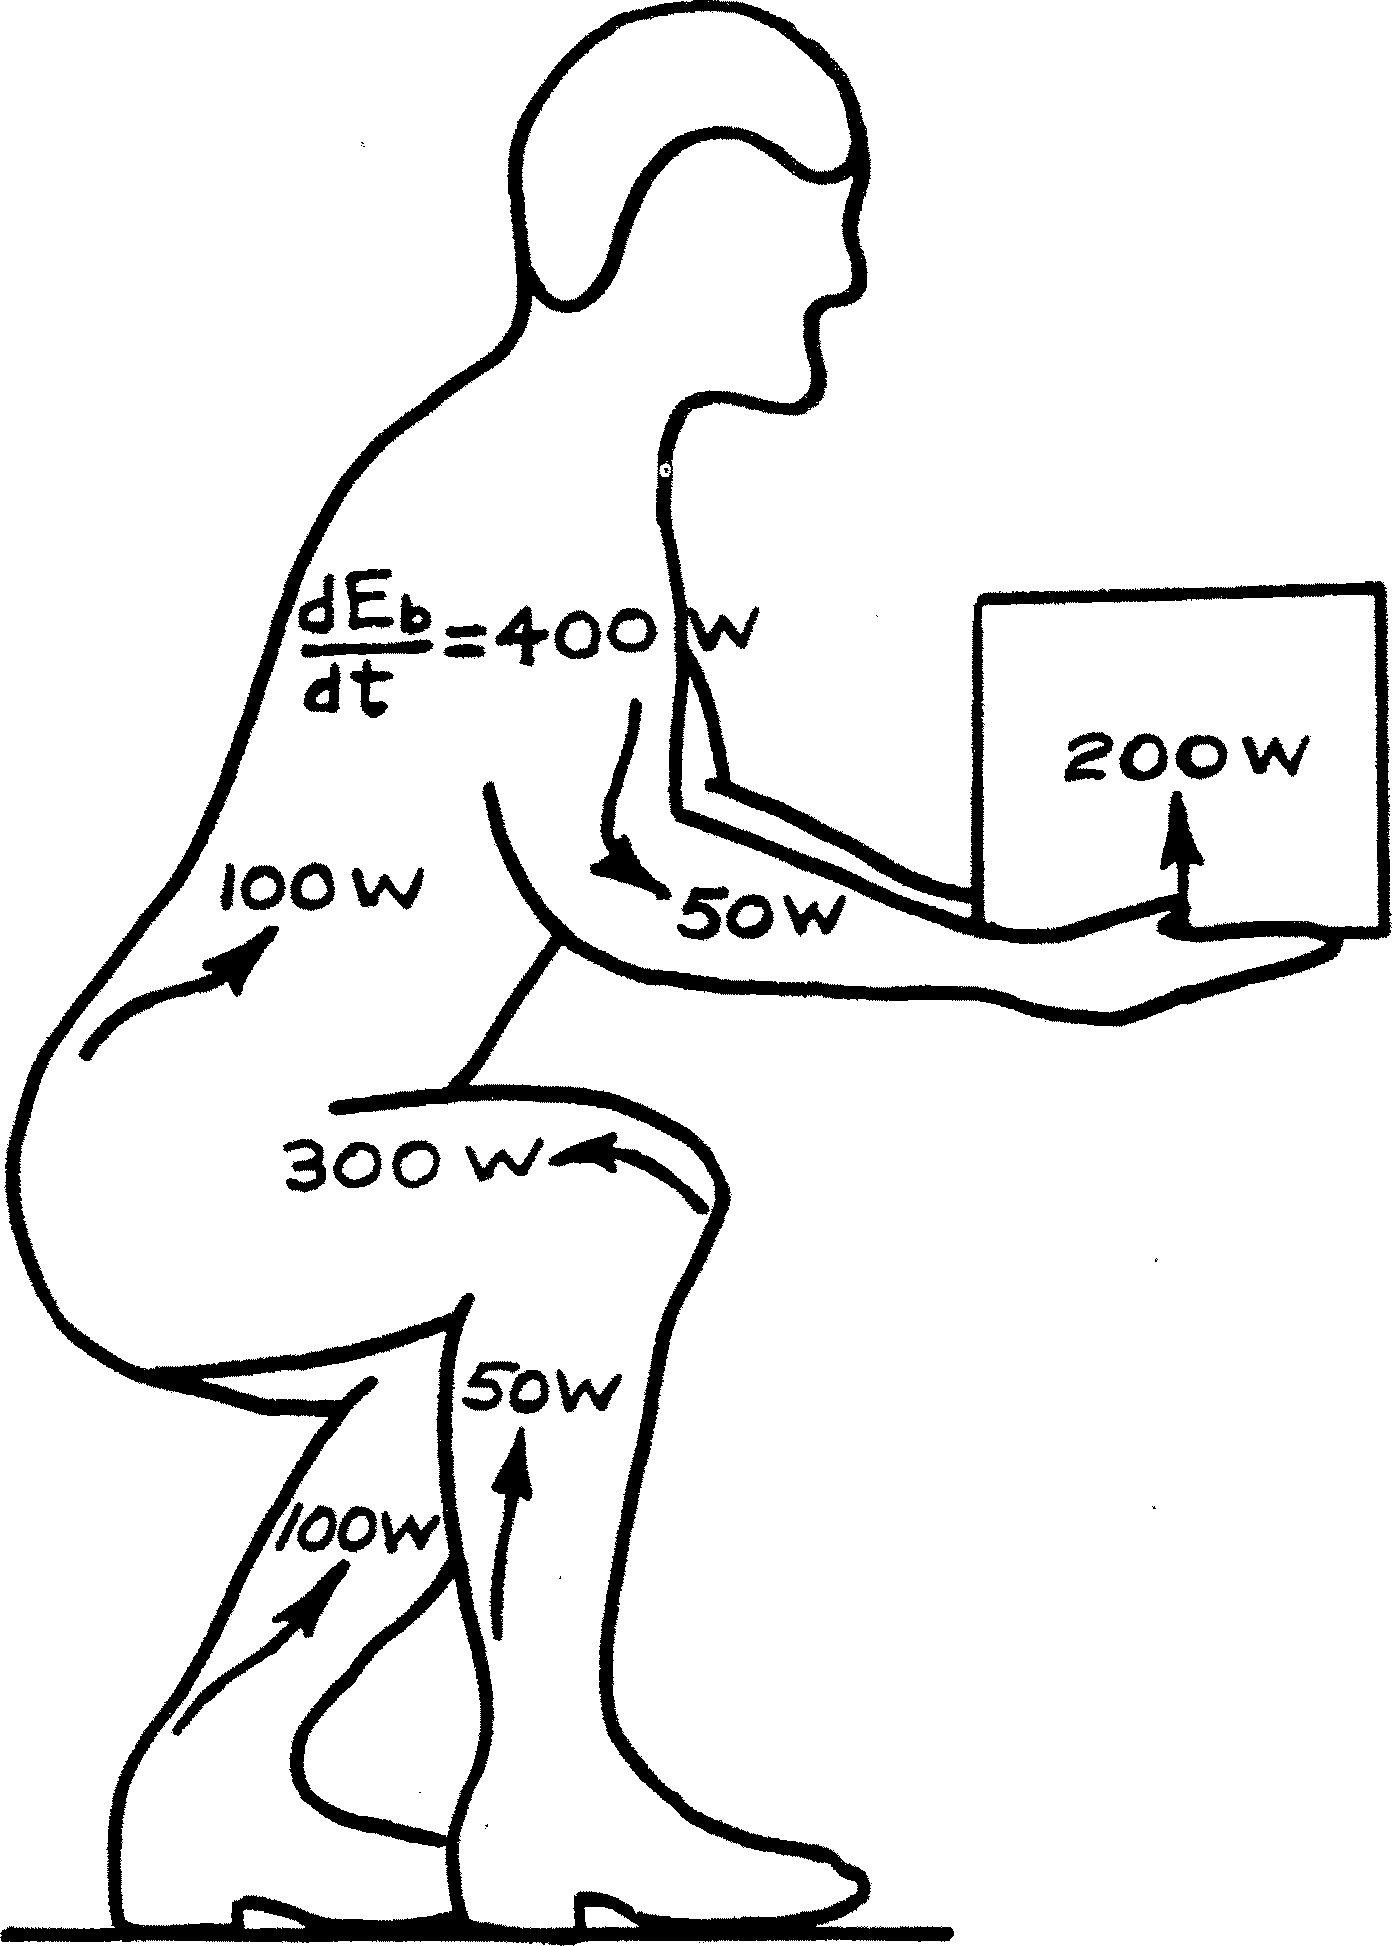
\includegraphics[width=0.45\textwidth]{610.png}
  \caption{Trabajo «interno» frente a «externo» al levantar un objeto (De \cite{107}. Reimpreso con autorización de Wiley).}
  \label{fig:610}
\end{SCfigure}



Al discutir las tasas metabólicas debemos ser cuidadosos al definir los tipos de trabajo y de energía \cite{107}. La Figura 6.10 muestra que al levantar un objeto, lo cual podemos llamar trabajo externo, también se realiza trabajo alrededor de las articulaciones del cuerpo para elevar el centro de masa del propio cuerpo, lo cual es trabajo interno. Asimismo, se dice que las contracciones musculares concéntricas realizan trabajo (mecánico) positivo, mientras que las contracciones excéntricas realizan trabajo negativo. Caminar sobre un terreno plano requiere cantidades iguales de trabajo positivo y negativo. Caminar cuesta arriba requiere relativamente más trabajo positivo, mientras que caminar cuesta abajo requiere relativamente más trabajo negativo. Las eficiencias de trabajo del trabajo positivo y del trabajo negativo son diferentes.

El término eficiencia puede significar cosas diferentes, por lo que en general debemos ser cuidadosos y observar qué se está definiendo \cite{105,107}. La eficiencia metabólica o muscular es el trabajo mecánico total realizado por todos los músculos dividido por el trabajo metabólico realizado por los músculos. Otra medida de la eficiencia es la eficiencia mecánica, que es el trabajo mecánico total realizado (interno + externo) dividido por el costo de energía metabólica que excede al costo metabólico en reposo. Un parámetro más restrictivo es la eficiencia del trabajo, que es el trabajo mecánico externo dividido por el costo metabólico en exceso sobre el costo metabólico de trabajo cero. La ineficiencia se debe a la conversión incompleta de la energía metabólica en energía mecánica y a la ineficiencia neurológica en el control de esta energía mecánica.

Para nuestros propósitos, definiremos simplemente la eficiencia, $\epsilon$, como la tasa de realización de trabajo mecánico dividida por la tasa metabólica. Las Tablas 6.32 y 6.33 muestran que rara vez supera el $20\%$ y suele ser mucho menor que esto. El ciclismo es relativamente eficiente, con una $\epsilon$ que se aproxima al $22\%$ para los ciclistas de carreras. El vagoneteo también es eficiente. (Esto implica empujar vagonetas cargadas con carbón a lo largo de una vía ferroviaria). Palear arena, una actividad más común, tiene solo una eficiencia del $3\%$. En comparación, las máquinas de vapor tienen una eficiencia del $17\%$ y los motores de gasolina tienen una $\epsilon = 38\%$.

\begin{table}[htbp]
\centering
\caption{Potencia mecánica y eficiencia del trabajo mecánico}
\label{tab:632}
\small
\begin{tabularx}{0.8\textwidth}{X >{\centering\arraybackslash}c >{\centering\arraybackslash}c >{\centering\arraybackslash}c >{\centering\arraybackslash}c}
\toprule
\textbf{Tarea} & \multicolumn{2}{c}{\textbf{Potencia mecánica de salida}} & \textbf{Tasa metabólica} & \textbf{Eficiencia} \\
\cmidrule(lr){2-3}
 & \textbf{(hp)} & \textbf{(W)} & \textbf{(W)} & \textbf{(\%)} \\
\midrule
Ciclismo (típico) & 0,15 & 112 & 505 & 19 \\
Vagoneteo & 0,12 & 90 & 525 & 17 \\
Palear arena & 0,024 & 17,5 & 570 & 3 \\
\bottomrule
\end{tabularx}
\begin{flushleft}
    \small Utilizando datos de \cite{9}.
\end{flushleft}
\end{table}

\begin{table}[htbp]
\centering
\caption{Eficiencias del trabajo mecánico}
\label{tab:633}
\small
\begin{tabularx}{0.7\textwidth}{X >{\centering\arraybackslash}c}
\toprule
\textbf{Actividad de ejercicio o tarea} & \textbf{Eficiencia (\%)} \\
\midrule
Ciclismo, nivelado & 24\text{--}34 \\
Ciclismo, cuesta arriba & 19 \\
Patinaje sobre hielo & 11 \\
Remo & 10\text{--}20 \\
Máquina escaladora & 23 \\
Natación, estilo libre & 2,9\text{--}7,4 \\
Caminar, horizontal & 20\text{--}35 \\
Caminar, con inclinación & 21\text{--}43 \\
\bottomrule
\end{tabularx}
\begin{flushleft}
    \small Utilizando datos de \cite{35}.
\end{flushleft}
\end{table}

¿A dónde va el resto de la energía? El resto se destina a la producción de calor. Esto significa que del $80\text{ al }100\%$ del producto final de su metabolismo es calor; este número suele estar más cerca del $100\%$. En cualquier caso, los $\sim 500\text{ kcal}$ de trabajo mecánico realizado por un trabajador físico durante un día se traducen en necesidades dietéticas de al menos $2500\text{ kcal}$ por encima de la BMR, porque la eficiencia mecánica suele ser $<20\%$.

La tasa de captación de oxígeno está limitada por la tasa en la que los pulmones pueden absorber oxígeno y la velocidad a la que el corazón puede distribuir este oxígeno por todo el cuerpo para el metabolismo aeróbico.

\begin{table}[htbp]
\centering
\caption{Récords mundiales de velocidad en carrera}
\label{tab:634}
\small
\begin{tabularx}{0.6\textwidth}{X >{\centering\arraybackslash}c}
\toprule
\textbf{Distancia (m)} & \textbf{Velocidad promedio de carrera (m/s)} \\
\midrule
100 & 10,44 \\
200 & 10,42 \\
400 & 9,26 \\
1500 & 7,28 \\
10\,000 & 6,34 \\
42\,195$^{\text{a}}$ & 5,72 \\
100\,000 & 4,46 \\
\bottomrule
\end{tabularx}
\begin{flushleft}
    \small $^{\text{a}}$ Maratón, $26\text{ millas}$, $385\text{ yd}$.\\
    Datos de 2014.
\end{flushleft}
\end{table}

Un ejemplo de esto es la disminución en la velocidad de carrera humana al aumentar la distancia (más allá de $\sim 200\text{ m}$), lo cual se debe a las limitaciones en la captación de oxígeno. Esto queda claro a partir de las velocidades promedio de carrera récord mundial para diversas distancias que se muestran en la Tabla 6.34.

\begin{SCfigure}[0.9][htbp]
  \centering
  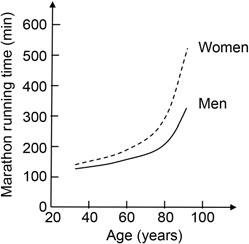
\includegraphics[width=0.5\textwidth]{611.png}
  \caption{Variación de los mejores tiempos de maratón con la edad (basado en \cite{99}).}
  \label{fig:611}
\end{SCfigure}



Los tiempos de clase mundial al correr cada uno de estos eventos aumentan con la edad, manteniéndose el rendimiento máximo hasta los $\sim 35\text{ años}$ de edad y luego disminuye, primero lentamente hasta los $\sim 50\text{--}60\text{ años}$ de edad y luego más rápido, con disminuciones más rápidas en eventos de resistencia que en velocidad. Esto se observa en la Figura 6.11 para quienes corren maratones \cite{99}.

\begin{SCfigure}[0.8][htbp]
  \centering
  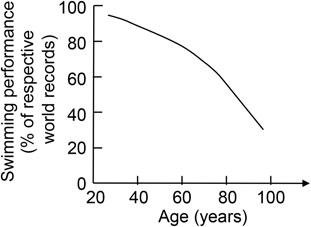
\includegraphics[width=0.55\textwidth]{612.png}
  \caption{Variación de los mejores tiempos de natación con la edad, para carreras de $50\text{ y }1500\text{ m}$, para hombres y mujeres (basado en \cite{99}).}
  \label{fig:612}
\end{SCfigure}



Aun así, los tiempos ganadores en los Juegos Olímpicos de 1896 (los primeros Juegos Olímpicos modernos, en Atenas) son alcanzados actualmente por corredores de clase mundial que tienen aproximadamente $60\text{ años}$ de edad \cite{99}. El rendimiento máximo en natación también disminuye con la edad avanzada, pero a ritmos comparables para eventos de velocidad y resistencia (Figura 6.12) \cite{28,99}.

La Tabla 6.35 muestra que la potencia máxima de trabajo mecánico que puede realizar una persona bien acondicionada disminuye con la duración de la tarea. Durante tiempos cortos podemos realizar trabajo mecánico a una tasa más alta debido a los procesos metabólicos anaeróbicos; el trabajo a más largo plazo requiere procesos aeróbicos.

\begin{table}[htbp]
\centering
\caption{Potencia mecánica máxima aproximada de seres humanos bien acondicionados}
\label{tab:635}
\small
\begin{tabularx}{\textwidth}{X >{\centering\arraybackslash}c >{\centering\arraybackslash}c >{\centering\arraybackslash}c >{\centering\arraybackslash}c}
\toprule
\multicolumn{2}{c}{\textbf{Potencia}} & \textbf{Duración} & \multicolumn{2}{c}{\textbf{Energía total}} \\
\cmidrule(lr){1-2} \cmidrule(lr){4-5}
\textbf{(hp)} & \textbf{(W)} & & \textbf{(kJ)} & \textbf{(kcal)} \\
\midrule
2 & 1500 & 6\text{ s} & 9,0 & 2,2 \\
1 & 750 & 1\text{ min} & 45 & 10,8 \\
0,35 & 260 & 35\text{ min} & 546 & 130 \\
0,2 & 150 & 5\text{ h} & 2700 & 645 \\
0,1 & 75 & Jornada de $8\text{ h}$ de un trabajador & 2160 & 516 \\
\bottomrule
\end{tabularx}
\begin{flushleft}
    \small Utilizando datos de \cite{9}. Véase también \cite{105}.
\end{flushleft}
\end{table}

\subsubsection*{Cómo «quemar» la comida}

Supongamos que acaba de comer una dona «estándar». Se siente culpable y quiere quemar esas calorías adicionales. ¿Qué puede hacer?

Si está sentado en reposo, está quemando de forma natural $\sim 103\text{ kcal/h}$ (hombre de $70\text{ kg}$). Si decide jugar al baloncesto, su tasa metabólica aumenta a $\sim 688\text{ kcal/h}$, por lo que estará incrementando su tasa metabólica en $\sim 585\text{ kcal/h}$. Quemará esa dona estándar de $280\text{ kcal}$ en
\begin{equation}
\frac{280\text{ kcal}}{585\text{ kcal/h}} = 0{,}48\text{ h} = 29\text{ min}.
\label{eq:633}
\end{equation}

Esa dona le costará media hora de baloncesto a un ritmo verdaderamente intenso.

Supongamos que quiere «bajar» esa dona caminando. La tasa metabólica durante una caminata lenta es de $\sim 228\text{ kcal/h}$, la cual excede a la de estar sentado en reposo por $\sim 125\text{ kcal/h}$. Para bajar esa dona caminando tendría que caminar durante
\begin{equation}
\frac{280\text{ kcal}}{125\text{ kcal/h}} = 2{,}24\text{ h} = 2\text{ h } 14\text{ min}.
\label{eq:634}
\end{equation}

Lo cual es un poco más largo que la mayoría de los paseos después de la cena.

¿Por qué las personas aumentan de peso a medida que envejecen? Una razón es la disminución de la BMR con la edad (Tablas 6.19 y 6.20). El nivel de actividad $f_{\text{av}}$ a menudo disminuye con la edad. Además, a veces las personas comen más (picoteo) (véase el Problema 6.88). Ahora examinaremos cómo se combinan la ingesta calórica y la actividad para determinar el peso corporal.

\subsection{Pérdida y ganancia de peso}

Si su tasa de ingesta calórica supera su tasa metabólica, usted aumenta de peso. Si es menor, pierde peso. Puede controlar su ingesta calórica controlando lo que se lleva a la boca. Tiene cierto control sobre su tasa metabólica al ser más o menos activo en general y al hacer más o menos ejercicio. (En un atrevido ejemplo de su devoción a la ciencia y a sus lectores, mientras escribía la primera edición de este texto, el autor demostró lo fácil que es ganar $10\text{ lb}$ en $6\text{ meses}$ simplemente haciendo menos ejercicio y picando más por la noche. ¡No necesitó suplementos dietéticos para lograr esta hazaña! El autor consideró el experimento inverso de pérdida de peso mediante más ejercicio y menos picoteo. Al momento de escribir esta segunda edición, todavía estaba considerando este experimento). Como veremos más adelante en este capítulo, su tasa metabólica está relacionada con su temperatura corporal y la pérdida de calor corporal. Por ejemplo, si tiene mucho frío, tiembla y esto aumenta su TM.

Aquí y en los problemas examinaremos algunos modelos muy sencillos de pérdida y ganancia de peso. ¿Cuánto peso en forma de grasa corporal se puede perder realmente en una semana? ¿Cómo se controla el peso corporal mediante la ingesta de sal? ¿Cómo varía su peso corporal debido a cambios en la ingesta calórica, la edad y la estatura específica? Nuestros modelos no solo son sencillos, son demasiado simplistas y, sin embargo, es un poco difícil hacerlos más realistas. Por ejemplo, los aumentos de peso corporal debido al músculo añadido incrementan la BMR mucho más que aquellos debidos a la grasa añadida. ¿Cómo se puede incluir esto en el modelo?

\begin{figure}[htbp]
  \centering
  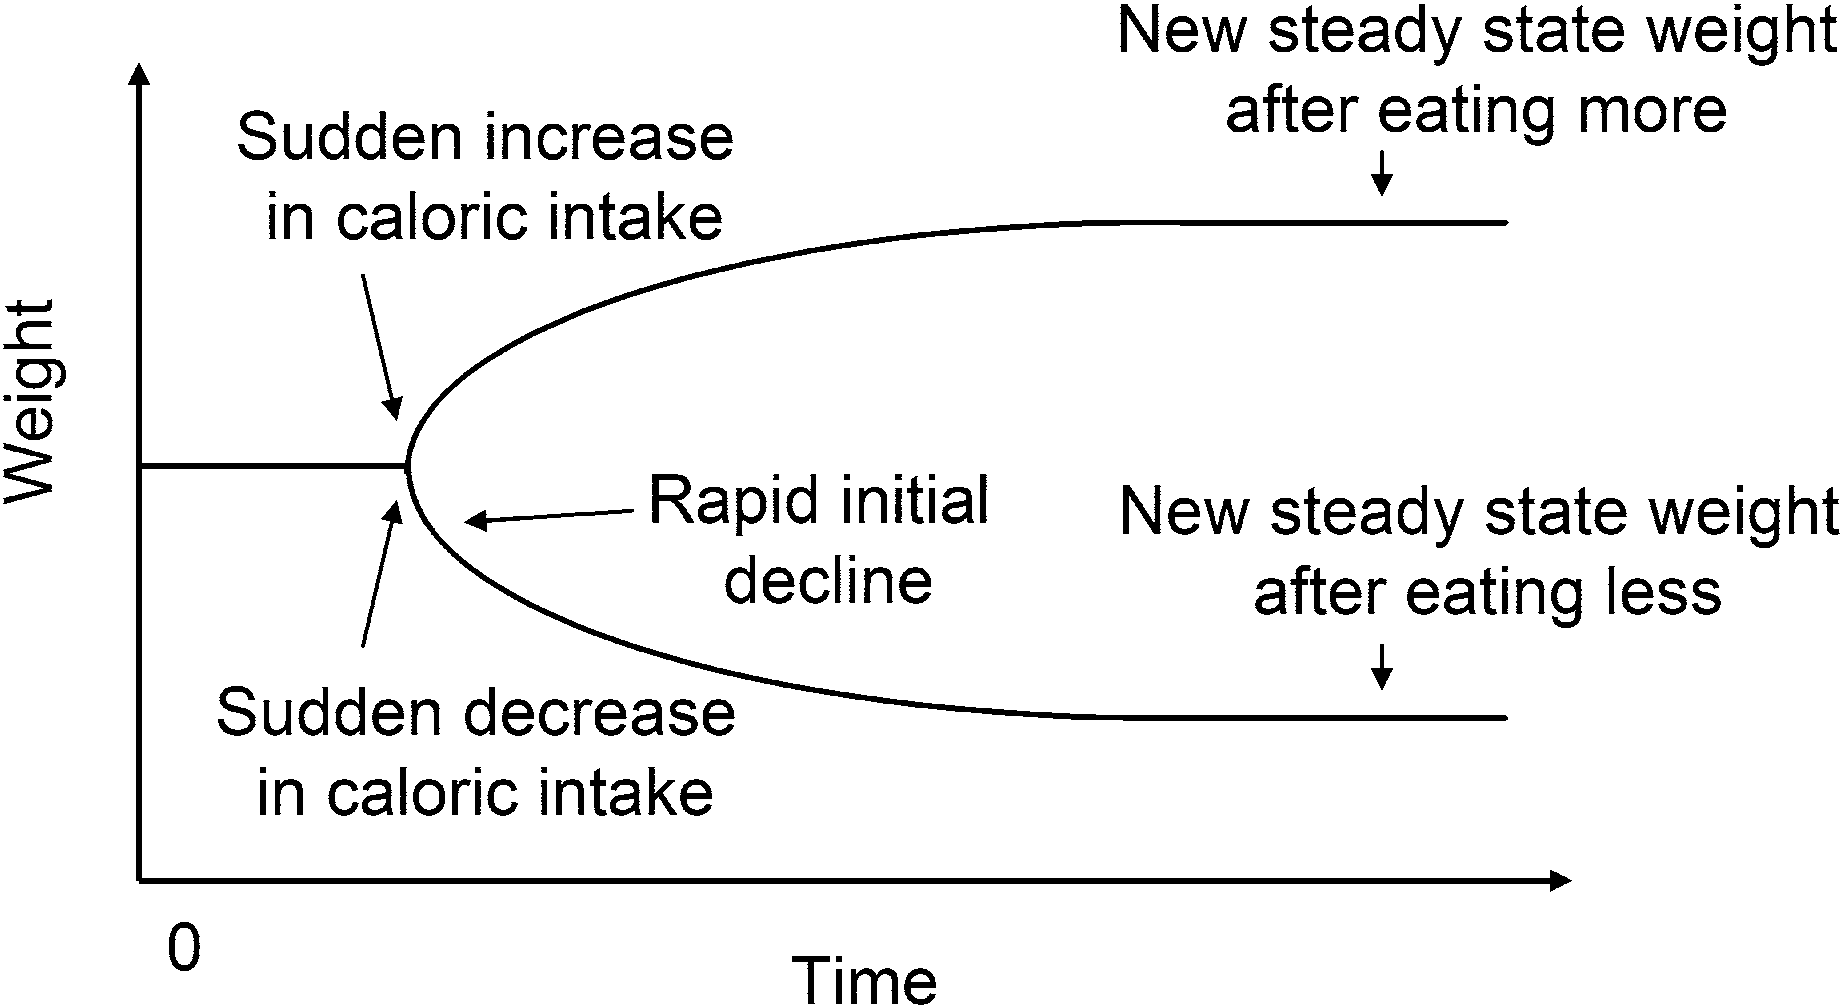
\includegraphics[width=0.8\textwidth]{613.png}
  \caption{Esquema de la evolución temporal de la ganancia o pérdida de peso ante un pequeño aumento o disminución repentino en la ingesta metabólica (que luego se mantiene en este nuevo nivel). Se esperan cambios similares para una pequeña disminución o aumento repentino en el nivel de actividad, respectivamente.}
  \label{fig:613}
\end{figure}



¿Es razonable aplicar las relaciones que caracterizan cómo depende la tasa metabólica promedio del peso corporal, la edad y la estatura utilizando la Ley de Kleiber, las ecuaciones de Harris--Benedict, etc., para determinar el peso en estado estacionario y los cambios de peso para un individuo dado? No está claro que sea razonable. Como se señaló anteriormente, estos son promedios sobre grupos de personas y no tendencias para una persona en particular. El cuerpo controla las tasas metabólicas de manera diferente para distintos individuos en respuesta a estímulos como la dieta, lo que hace que para algunos sea más fácil perder peso, mientras que para otros sea más difícil. Aun así, por ahora, asumamos que estas relaciones también se aplican a un individuo determinado y que, por lo tanto, pueden usarse para determinar cómo cambia el peso en estado estacionario de una persona con la ingesta de alimentos, el nivel de actividad y la edad. Ante un cambio repentino en la ingesta metabólica o la actividad hacia un nuevo nivel, ¿qué tan rápido alcanza el cuerpo su nuevo estado estacionario? Los cambios generales se representan en la Figura 6.13.

Si su ganancia o pérdida de peso involucrara únicamente grasa, el valor calórico de la grasa de $9\text{ kcal/g}$ significa que un aumento o disminución en la ingesta metabólica de $4090\text{ kcal}$ resultaría en una ganancia o pérdida de una libra (de grasa). Si su cambio de peso involucrara solo proteínas ($4\text{ kcal/g}$), un cambio de $1820\text{ kcal}$ cambiaría la masa corporal en una libra. Según la regla de Wishnofsky, cuando usted aumenta o disminuye su ingesta metabólica en $3500\text{ kcal}$, gana o pierde aproximadamente una libra \cite{108}. En consecuencia, la regla de Wishnofsky sugiere que la ganancia o pérdida promedia típicamente alrededor de $3/4$ de grasa y $1/4$ de músculo.

Debido a las diferentes masas de músculo, grasa y líquidos en hombres y mujeres, y en personas jóvenes y mayores, hoy en día no se considera que esta regla tan utilizada sea realmente universal. Este contenido energético promedio del cambio de peso es en realidad significativamente menor para los hombres ($2480\text{ kcal/lb}$) que para las mujeres ($3380\text{ kcal/lb}$). Además, es aproximadamente un $10\%$ mayor para las personas mayores ($2610\text{ kcal/lb}$ para hombres de $70\text{ años}$; $3510\text{ kcal/lb}$ para mujeres de $70\text{ años}$) que para las personas más jóvenes ($2360\text{ kcal/lb}$ para hombres de $35\text{ años}$; $3260\text{ kcal/lb}$ para mujeres de $35\text{ años}$) \cite{79}. (Todos estos valores han sido escalados para la misma persona de $90\text{ kg}$ y $170\text{ cm}$ de estatura).

Supongamos que aumenta o disminuye su ingesta de alimentos en $1000\text{ kcal/día}$. Si todo esto se destinara a aumentar o disminuir sus reservas de grasa, esto llevaría a un cambio de $1000\text{ kcal/día}$ dividido por $9\text{ kcal/g}$ de grasa, o aproximadamente $110\text{ g}$ de grasa al día, lo que corresponde a $1/4\text{ lb}$ por día o aproximadamente $2\text{ lb}$ por semana. Si está a dieta, una disminución en la ingesta calórica de $1000\text{ kcal/día}$ es muy grande, por lo que nunca puede esperar perder más de $2\text{ lb}$ a la semana. (Por supuesto, el ejercicio regular también aceleraría la pérdida de peso).

¿Por qué algunas dietas prometen una pérdida de peso más rápida, especialmente al principio? Algunas dietas pueden implicar en realidad la pérdida de agua corporal, con muy poca pérdida de grasa, carbohidratos o proteínas. (Los boxeadores que necesitan perder peso rápidamente para entrar en una categoría de peso a menudo siguen este tipo de dietas). Además, la pérdida de peso en una dieta legítima puede ser muy rápida al principio. En los primeros días de dieta, quemar $1000\text{ kcal}$ implica quemar glucógeno de la pequeña reserva de glucógeno. Quemar glucógeno consume $4{,}1\text{ kcal/g de glucógeno}$, pero debido a la pérdida concomitante de agua asociada con el glucógeno, solo se consume aproximadamente $1\text{ kcal}$ por gramo total perdido. Por lo tanto, se pierden $1000\text{ kcal} / (1\text{ kcal/g}) = 1000\text{ g}$, lo que equivale a unas $2\text{ lb}$. Más tarde, cuando en su lugar se oxida grasa, este mismo déficit de $1000\text{ kcal}$ resulta en una pérdida de masa de solo $110\text{ g}$ ($1/4\text{ lb}$). Este ritmo de pérdida de peso repentinamente más lento (en la aproximación al nuevo peso en estado estacionario) puede desanimar fácilmente a quienes hacen dieta.

Para parafrasear el consejo dado por el Sr. Micawber a David Copperfield de Charles Dickens: «Ingesta calórica diaria de $2000\text{ kcal}$, gasto de energía diario de $2100\text{ kcal}$, resultado: felicidad. Ingesta calórica diaria de $2000\text{ kcal}$, gasto de energía diario de $1900\text{ kcal}$, resultado: miseria». (Esto es cierto al menos para aquellos que han dejado atrás sus años universitarios).

La ingesta y el gasto de energía claramente afectan el peso corporal de esta manera directa. Sin embargo, varios factores que no se comprenden muy bien parecen influir en la ingesta y el gasto de energía y, por consiguiente, en el peso corporal \cite{56}. Los genes son uno de varios factores que causan la obesidad \cite{101}. Algunos genes regulan el apetito, y con la fácil disponibilidad de alimentos digeribles y altamente calóricos, aquellos con genes que aumentan el apetito pueden ganar peso más fácilmente. El estrés crónico incrementan el nivel en estado estacionario de la hormona cortisol, lo que aumenta el apetito por alimentos densos en calorías, económicos y muy apetecibles, como la «comida chatarra» \cite{1}. El aumento del ejercicio mejora la condición cardiovascular (y su tasa de mortalidad por muchas enfermedades \cite{12}), pero no siempre reduce considerablemente el peso corporal \cite{13,25,81}. El incremento neto en la tasa metabólica promedio debido al ejercicio reduce su peso en estado estacionario, pero no necesariamente lo suficiente como para mantener una gran pérdida de peso a largo plazo. Aumentar la masa muscular mediante el ejercicio, a expensas de la grasa, incrementará su BMR y conducirá a cierta pérdida de peso. Sin embargo, el aumento de ejercicio a veces se acompaña de un mayor deseo de comer. Las personas mayores con obesidad parecen perder peso cuando siguen una dieta controlada, hagan o no ejercicio, y no pierden peso solo con el aumento del ejercicio o sin dieta ni ejercicio \cite{102}. Estudios más amplios en personas con obesidad sugieren que la combinación de dieta y ejercicio conduce a una mayor pérdida de peso que cualquiera de los dos por separado \cite{48}. Si usted duerme muy poco, su tasa metabólica diaria aumenta, lo que se esperaría que disminuyera su peso. Sin embargo, parece que su cuerpo lo convence de comer más alimentos, tanto que sobrecompensa su mayor tasa metabólica y en realidad aumenta de peso \cite{8,61}. Sorprendentemente, la TM (o TEE) de los occidentales y de los cazadores-recolectores es aproximadamente la misma para la misma masa corporal (o masa corporal libre de grasa), por lo que el aumento de la ingesta calórica de los occidentales es probablemente más importante como causa de obesidad en algunos que su sospechado, pero no probado, menor gasto energético \cite{82}.

Otros aspectos del metabolismo, la dieta y el control del peso tampoco se comprenden bien. Aunque el ejercicio parece ayudar directamente con el control de peso al aumentar la tasa metabólica, puede afectarlo indirectamente a través de cómo el cuerpo controla las rutas y la eficiencia del metabolismo de los alimentos. En cualquier caso, el ejercicio generalmente no sustituye el control de la cantidad y el tipo de alimentos ingeridos \cite{67}. Existe evidencia de que una dieta alta en proteínas y de bajo índice glucémico ayuda a mantener la pérdida de peso, mientras que una dieta baja en proteínas y de alto índice glucémico no lo hace \cite{54}. Además, el cuerpo convierte la grasa marrón (not la grasa blanca habitual y más abundante) en calor aparentemente sin alimentar las actividades metabólicas; parece ser una fuente de calor para los bebés cuando tienen frío, antes de que su mecanismo de tiritar esté activo. Los adultos también parecen tener cierta cantidad de grasa marrón. Es posible que la creación y el metabolismo de la grasa marrón sean importantes para controlar el equilibrio energético corporal en algunos adultos, incluso bajo condiciones en las que las tasas metabólicas suelen ser más lentas, como cuando las personas están inactivas y cuando hace fresco (temperaturas más bajas, pero no lo suficiente como para causar tiritones) \cite{74}.

Existe cierta evidencia de que comer alimentos específicos puede afectar el peso corporal, aunque las razones de esto no siempre están claras. Decidir incluir cacahuates (maníes) y frutos secos, como las almendras, como parte de su dieta puede ayudar a controlar o incluso reducir el peso corporal \cite{64}. Los frutos secos son saciantes debido a su alto contenido de proteínas y fibra, y tal vez a su alto contenido de grasa, y este efecto saciante reduce la ingesta calórica posterior en un $\sim 55\text{--}75\%$ de la energía que supuestamente aportan los frutos secos. Se digiere una fracción menor del contenido calórico de los frutos secos enteros en comparación con el de la mantequilla y el aceite de frutos secos, perdiéndose posiblemente un $\sim 10\text{--}15\%$ o más del contenido calórico en las heces. El contenido de energía utilizable de las almendras puede ser de $\sim 4{,}8\text{ kcal/g}$, en comparación con el valor de $6{,}0\text{--}6{,}1\text{ kcal/g}$ obtenido mediante los factores de Atwater \cite{76}. Además, existe alguna evidencia de que el consumo crónico de frutos secos puede aumentar la BMR, tal vez en aproximadamente un $10\%$. Esto todavía no es seguro.

Las calorías baratas están disponibles para muchos en los países desarrollados, y esta disponibilidad ha aumentado en los últimos siglos. Por ejemplo, el número de calorías disponibles per cápita en Inglaterra y Gales aumentó de un estimado de $\sim 2230\text{ kcal}$ en 1700 a $\sim 2980\text{ kcal}$ en 1910 \cite{34}. Un problema importante para mantener pesos corporales deseables es que las calorías baratas (en la sabrosa comida chatarra) están demasiado disponibles.

Para la mayoría de las personas en los países desarrollados obtener suficientes calorías diarias a partir de alimentos densos en calorías no es un problema, pero esto no es cierto a nivel mundial ni durante las guerras, when transportar suficientes calorías para los soldados y suministrar calorías a los civiles puede ser muy importante. Los cambios estacionales en el peso corporal ocurren en personas que realizan trabajo físico estacional y que no tienen acceso a una fuente constante de alimentos ricos en calorías. Por ejemplo, los agricultores en Gambia pierden peso ($\sim 10\text{ lb}$ o $\sim 5\text{ kg}$) durante la temporada de lluvias y siembra y, si la cosecha es exitosa, lo recuperan durante la temporada seca de cosecha y descanso \cite{56,84,93}. Aquellos con carreras que implican mucho trabajo físico, como agricultores, carpinteros y atletas profesionales, deben disminuir su ingesta calórica diaria después de jubilarse o aumentarán mucho de peso, a menos que hagan mucho más ejercicio \cite{56}.

¿Por qué las personas se han vuelto más altas con cada generación en muchos países desarrollados? Cuando la ingesta calórica de los niños es limitada, gran parte se utiliza para actividades metabólicas básicas y actividades adicionales (que podrían implicar mucho trabajo físico) y para combatir enfermedades, y se utiliza menos de lo necesario para el crecimiento. Con una mayor ingesta calórica (y a veces menos trabajo físico), se puede destinar más energía al crecimiento y las personas pueden alcanzar la estatura determinada por sus genes \cite{56}. (Con un exceso de ingesta calórica, también engordan).

Desde el punto de vista de la salud, a veces se cita el IMC ideal como $25\text{ kg/m}^2$, pero esto parece ser cierto solo para hombres con estaturas de $\sim 1{,}75\text{ m}$ ($5'\ 9''$) y es mayor, $\sim 26\text{ kg/m}^2$, para hombres más bajos ($<1{,}68\text{ m}$, $5'\ 6''$) y menor, de $22\text{ a }24\text{ kg/m}^2$, para hombres más altos ($>1{,}83\text{ m}$, $6'$) \cite{34}. Los IMC de los hombres estadounidenses de entre cuarenta y cincuenta años aumentaron de $\sim 22$ a más de $27\text{ kg/m}^2$ entre 1870 y 2000, por lo que ahora muchos hombres tienen un IMC por encima del umbral actual de $25\text{ kg/m}^2$ para el sobrepeso \cite{34,56}. (Solo una parte de este aumento puede atribuirse a los aumentos observados en la estatura y a cómo el IMC presume que la masa corporal idealmente se escala cuadráticamente con la estatura (véase el Problema 1.42)).

El IMC parece afectar la esperanza de vida. La mortalidad para hombres y mujeres noruegos de entre $50\text{ y }64\text{ años}$ es bastante constante para aquellos con IMC entre $21\text{ y }29$, pero aumenta rápidamente para aquellos con IMC progresivamente menores de $21$ (demasiado delgados) o progresivamente mayores de $29$ (demasiado obesos) \cite{34,103}.

\begin{figure}[htbp]
  \centering
  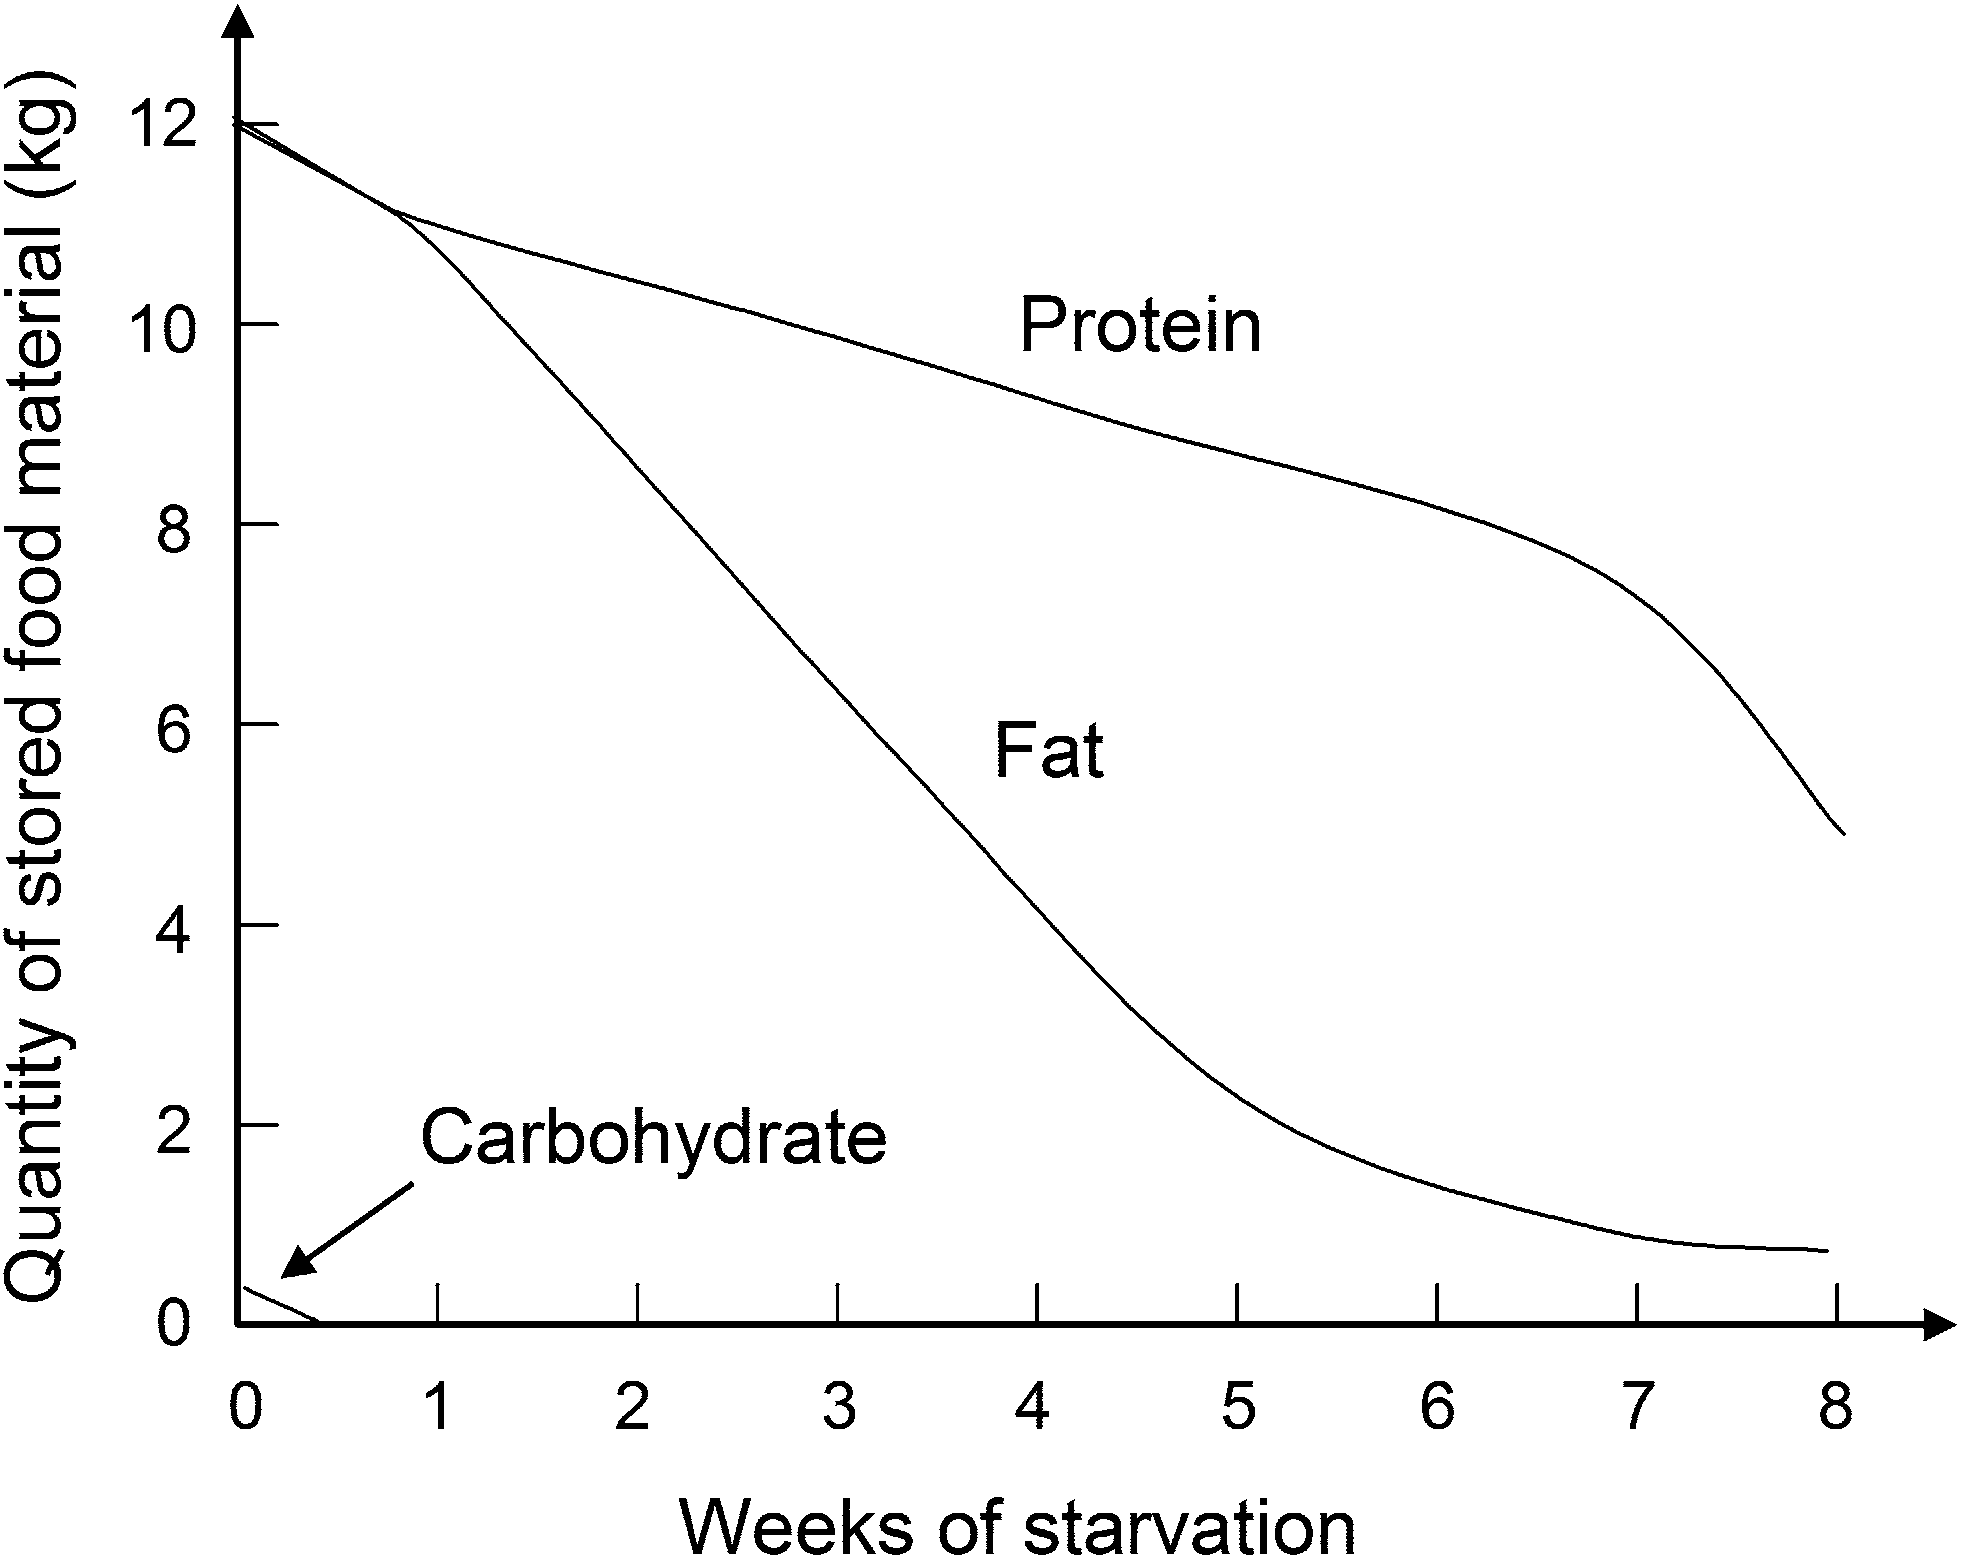
\includegraphics[width=0.7\textwidth]{614.png}
  \caption{Efecto de la inanición en las reservas de energía en el cuerpo (basado en \cite{45}).}
  \label{fig:614}
\end{figure}



Durante la inanición, el cuerpo utiliza primero todos los carbohidratos disponibles —principalmente el glucógeno en el hígado y los músculos— y esto satisface las necesidades energéticas del cuerpo durante aproximadamente medio día. Luego, el cuerpo agota las grasas y proteínas (véase la Figura 6.14); las reservas de grasa son aproximadamente $100$ veces mayores que las reservas iniciales de carbohidratos. Luego, sin grasa restante, las proteínas se siguen consumiendo hasta la muerte. La muerte ocurre cuando se ha agotado aproximadamente la mitad de las proteínas, debido a que estas son necesarias para la función celular.

\section{Pérdida de calor corporal}

¿Por qué es importante la pérdida de calor corporal? Prácticamente todo nuestro metabolismo se convierte en calor, debido a que normalmente muy poca energía se destina a trabajo mecánico útil. Considere la BMR de una persona con $m_{\text{b}} = 70\text{ kg}$, que es de $\sim 1680\text{ kcal/día}$. Esto se traduce en $70\text{ kcal/h}$. Utilizando (6.5), la velocidad con la que aumentaría la temperatura corporal con el tiempo si todo el calor permaneciera dentro del cuerpo es
\begin{equation}
\frac{dT}{dt} = \frac{1}{m_{\text{b}} c_{\text{b}}} \frac{dQ}{dt} = \frac{\text{BMR}}{m_{\text{b}} c_{\text{b}}},
\label{eq:635}
\end{equation}
donde la tasa de producción de calor $dQ/dt \approx \text{BMR}$ y el calor específico humano promedio es $c_{\text{b}} = 0{,}83\text{ kcal/kg-}^\circ\text{C}$. (Para ser consistentes con la literatura, usualmente expresaremos esto en términos de grados Kelvin en esta sección, que es $0{,}83\text{ kcal/kg-K}$). Esta capacidad calorífica es $C = 0{,}83\text{ kcal/kg-}^\circ\text{C} \times 70\text{ kg} = 58\text{ kcal/}^\circ\text{C}$. La velocidad de aumento de la temperatura es igual a
\begin{equation}
\frac{dT}{dt} = \frac{70\text{ kcal/h}}{58\text{ kcal/}^\circ\text{C}} = 1{,}2^\circ\text{C/h} = 2{,}1^\circ\text{F/h}.
\label{eq:636}
\end{equation}

Nuestra temperatura corporal aumentaría muy rápido sin modos efectivos de pérdida de calor, incluso con alguna producción de trabajo mecánico ($0{,}8\,\text{TM} < dQ/dt < \text{TM}$).

El calor específico del cuerpo se cita a menudo como $0{,}829\text{ kcal/kg-K}$. Esto es un poco más alto que el calculado utilizando el calor específico de cada componente del cuerpo, los cuales son (en $\text{kcal/kg-K}$) $0{,}507$ para los lípidos, $0{,}299$ para las proteínas, $0{,}201$ para la materia mineral, $0{,}272$ para los carbohidratos y $1{,}00$ para el agua. Estos valores calculados son de $0{,}798\text{ kcal/kg-K}$ para un hombre sin grasa (que contiene un $72\%$ de agua, $22\%$ de proteínas y $6\%$ de minerales en peso), $0{,}765\text{ kcal/kg-K}$ para un hombre delgado (que contiene un $12\%$ de grasa corporal) y $0{,}652\text{ kcal/kg-K}$ para un hombre obeso (que contiene un $50\%$ de grasa corporal). Las capacidades caloríficas de los diferentes tejidos corporales se muestran en la Tabla 6.36 y las de otros materiales comunes en la Tabla 6.37.

\begin{table}[htbp]
\centering
\caption{Características termofísicas de los tejidos y órganos corporales y de otros materiales}
\label{tab:636}
\small
\begin{tabularx}{\textwidth}{X >{\centering\arraybackslash}c >{\centering\arraybackslash}c >{\centering\arraybackslash}c}
\toprule
\textbf{Órgano o tejido} & \textbf{Conductividad térmica} & \textbf{Calor específico $c_{\text{v}}$} & \textbf{Densidad (aprox.)} \\
 & \textbf{$K$ (W/m-K)} & \textbf{(MJ/m$^3$-K)} & \textbf{$\rho$ (kg/m$^3$)} \\
\midrule
Piel: muy caliente & 2,80 & 3,77 & 1000 \\
Piel: mano normal & 0,960 & 3,77 & 1000 \\
Piel: fría & 0,335 & 3,77 & 1000 \\
Grasa pura subcutánea & 0,190 & 1,96 & 850 \\
Músculo: vivo & 0,642 & 3,94 & 1050 \\
Músculo: extirpado, fresco & 0,545 & 3,64 & 1050 \\
Hueso: promedio & 1,16 & 2,39 & 1500 \\
Hueso: compacto & 2,28 & 2,70 & 1790 \\
Hueso: trabecular & 0,582 & 2,07 & 1250 \\
Sangre: agua a 310 K & 0,623 & 4,19 & 993 \\
Sangre: plasma ($\text{Hct} = 0\%$) a 310 K & 0,599 & 4,05 & 1025 \\
Sangre: total ($\text{Hct} = 40\%$) & 0,549 & 3,82 & 1050 \\
Corazón: extirpado, casi fresco & 0,586 & 3,94 & 1060 \\
Hígado: extirpado, casi fresco & 0,565 & 3,78 & 1050 \\
Riñón: extirpado, casi fresco & 0,544 & 4,08 & 1050 \\
Núcleo del abdomen & 0,544 & 3,89 & 1050 \\
Cerebro: extirpado, casi fresco & 0,528 & 3,86 & 1050 \\
Cerebro: vivo & 0,805 & -- & -- \\
Pulmón: extirpado, bovino & 0,282 & 2,24 & 603 \\
Cuerpo entero (promedio) & -- & 4,12 & 1156 \\
\bottomrule
\end{tabularx}
\begin{flushleft}
    \small Tenga en cuenta que $1\text{ MJ/m}^3\text{-K} = 239\text{ kcal/m}^3\text{-K}$ y $1000\text{ kg/m}^3 = 1\text{ g/cm}^3$.\\
    Utilizando datos de \cite{38}.
\end{flushleft}
\end{table}

\begin{table}[htbp]
\centering
\caption{Características termofísicas de materiales}
\label{tab:637}
\small
\begin{tabularx}{\textwidth}{X >{\centering\arraybackslash}c >{\centering\arraybackslash}c >{\centering\arraybackslash}c}
\toprule
\textbf{Material} & \textbf{Conductividad térmica} & \textbf{Calor específico $c_{\text{v}}$} & \textbf{Densidad} \\
 & \textbf{$K$ (W/m-K)} & \textbf{(MJ/m$^3$-K)} & \textbf{$\rho$ (kg/m$^3$)} \\
\midrule
Aire & 0,009246 & 0,00119 & 1,18 \\
Tejido de algodón a 310 K & 0,0796 & 0,0267 & 160 \\
Caucho & 0,156 & 2,41 & 1200 \\
Etanol a 310 K & 0,163 & 1,96 & 789 \\
Teflón & 0,399 & 2,20 & 2180 \\
Hormigón & 0,934 & 1,93 & 2310 \\
Vidrio de placa & 1,09 & 1,94 & 2520 \\
Hielo a 249 K ($-42^\circ\text{C}$) & 2,21 & 1,76 & 913 \\
Zafiro (normal al eje c) a 310 K & 2\text{--}20 & 2,89 & 3970 \\
Acero inoxidable & 13,8 & 3,68 & 7910 \\
Aluminio & 204 & 2,45 & 2710 \\
Plata & 405 & 2,59 & 10500 \\
Diamante, natural & 2000 & 1,82 & 3510 \\
\bottomrule
\end{tabularx}
\begin{flushleft}
    \small Tenga en cuenta que $1\text{ MJ/m}^3\text{-K} = 239\text{ kcal/m}^3\text{-K}$ y $1000\text{ kg/m}^3 = 1\text{ g/cm}^3$.\\
    Utilizando datos de \cite{38}.
\end{flushleft}
\end{table}

\begin{figure}[htbp]
  \centering
  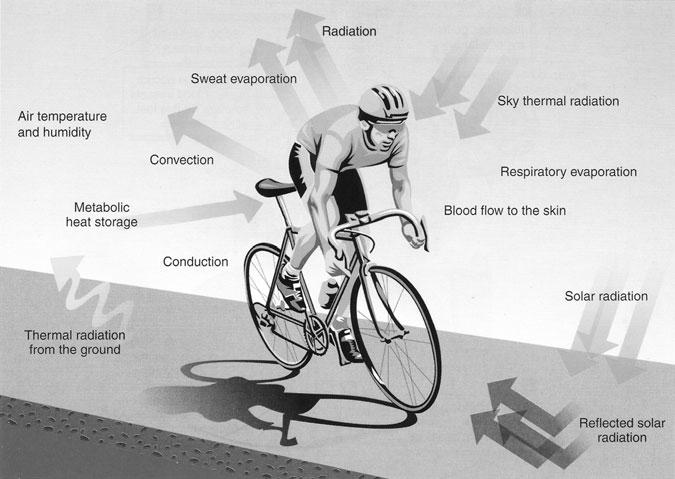
\includegraphics[width=0.7\textwidth]{615.png}
  \caption{Modos generales del cuerpo para la pérdida de calor y la ganancia de energía no metabólica (De \cite{106}, adaptado de \cite{43}. Utilizado con autorización).}
  \label{fig:615}
\end{figure}

\begin{SCfigure}[0.9][htbp]
  \centering
  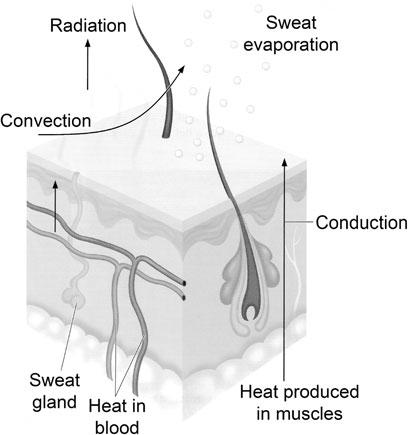
\includegraphics[width=0.5\textwidth]{616.png}
  \caption{Vista más microscópica de los modos de pérdida de calor por remoción desde la piel. Cuando la temperatura de la piel excede la temperatura ambiental, el calor se elimina mediante la evaporación del sudor, mientras que cuando es menor que la temperatura ambiental, hay una pérdida neta de calor únicamente por la evaporación del sudor. La piel es calentada por la sangre arterial y por conducción térmica a través del tejido subcutáneo (debajo de la piel) (De \cite{106}. Utilizado con autorización).}
  \label{fig:616}
\end{SCfigure}



\subsection{Modos de pérdida de calor}

Existen cuatros modos de pérdida de calor. Su magnitud absoluta y su importancia relativa dependen de la ropa, el entorno, el medio circundante, etc. (Figuras 6.15 y 6.16). Para discusiones generales sobre la pérdida de calor en personas, véanse \cite{10,11,19,35,106}.

\begin{enumerate}
\item La pérdida por radiación, también conocida como radiación de cuerpo negro, es la radiación térmica emitida por un objeto en equilibrio térmico. En reposo, normalmente entre el $54\text{ y }60\%$ de la pérdida de energía se produce a través de la radiación térmica.
\item La convección y la conducción del aire desde el cuerpo representan $\sim 25\%$ de la pérdida de calor.
\item La evaporación del sudor representa $\sim 7\%$ de la pérdida de calor.
\item La evaporación de agua a través de la respiración representa $\sim 14\%$ de esta pérdida.
\end{enumerate}

Durante una actividad muy intensa, la pérdida de calor aumenta desde el valor en reposo de $\sim 1{,}5\text{ a }\sim 15\text{ kcal/min}$. La cantidad debida a la radiación permanece aproximadamente igual, $0{,}8\text{ kcal/min}$, pero disminuye a aproximadamente el $5\%$ del total. La pérdida por conducción y convección aumenta de $\sim 0{,}3\text{ a }2{,}2\text{ kcal/min}$ y esto representa aproximadamente el $15\%$ de la pérdida total. Las pérdidas debidas a la evaporación del sudor aumentan de $\sim 0{,}3\text{ a }12{,}0\text{ mL/min}$ y constituyen aproximadamente el $80\%$ de la pérdida de calor.

Los principios de estos modos de pérdida de calor están determinados totalmente por la física; las magnitudes absolutas de la pérdida real pueden modificarse mediante procesos biológicos.

En los modelos sencillos de pérdida de calor, las personas a menudo se tratan como cilindros verticales, mientras que los animales de cuatro patas se modelan como cilindros horizontales. In particular, un hombre típico se modela como un cilindro de $1{,}65\text{ m}$ de altura con un diámetro de $0{,}234\text{ m}$. (Recuerde el comentario de la introducción de que, a orden cero, un físico podría modelar a una vaca como una esfera y que nuestros modelos aquí pueden volverse un poco más complejos; de hecho, un cilindro es más complejo que una esfera. Véase la Figura 1.33 para un modelo de un hombre compuesto por muchos componentes cilíndricos).

\begin{SCfigure}[0.75][htbp]
  \centering
  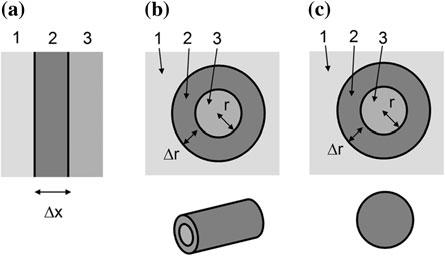
\includegraphics[width=0.6\textwidth]{617.png}
  \caption{Flujo térmico entre los medios 1 y 3, a través del medio 2, en diferentes geometrías: (a) placa rectangular, (b) corteza cilíndrica, (c) corteza esférica. En los casos comunes, $\Delta r$ es mucho menor que $r$.}
  \label{fig:617}
\end{SCfigure}



Nos centraremos principalmente en la pérdida de calor en una dimensión. Por ejemplo, la ecuación de conducción de calor (6.6) es unidimensional y describe el flujo de calor entre dos interfaces planas separadas por un espesor $\Delta x$ (Figura 6.17a). Matemáticamente, el flujo de calor radial a través de una corteza cilíndrica delgada de espesor $\Delta r$ en un cilindro de radio $r$ (Figura 6.17b) es idéntico al que cruza interfaces planas si la $\Delta x$ en (6.6) se reemplaza por $r \ln(1 + \Delta r/r)$. Para la conducción a través de una corteza esférica delgada de espesor $\Delta r$ en una esfera de radio $r$ (Figura 6.17c), debe reemplazarse por $r \Delta r / (r + \Delta r)$. En ambos casos, el parámetro reemplazado se reduce a $\Delta r$ cuando $r \gg \Delta r$, es decir, cuando la nueva interfaz se aproxima a un plano plano.

\subsubsection*{Pérdida de calor por radiación}

Los cuerpos en equilibrio térmico emiten un flujo específico de energía por unidad de área superficial y tiempo que depende de su temperatura. También reciben un flujo de radiación térmica del mundo exterior sobre su área superficial que depende de la temperatura de los alrededores.

Todos los objetos a una temperatura $T$ emiten dicha radiación térmica distribuida en un rango de longitudes de onda (o equivalentemente frecuencias) de acuerdo con la distribución de cuerpo negro de Planck para la intensidad, la cual es
\begin{equation}
I(\lambda, T) d\lambda = \frac{2 h c^2 \epsilon}{\lambda^5 \left[\exp\left(\frac{h c}{\lambda k_{\text{B}} T}\right) - 1\right]} d\lambda,
\label{eq:637}
\end{equation}
donde $\epsilon$ es un parámetro conocido como la emisividad, $h$ es la constante de Planck ($6{,}626 \times 10^{-34}\text{ J}\cdot\text{s}$), $k_{\text{B}}$ es la constante de Boltzmann ($1{,}381 \times 10^{-23}\text{ J/K}$) y $T$ es la temperatura en grados Kelvin (K) ($T(\text{K}) = T(^\circ\text{C}) + 273^\circ$). ($I(\lambda, T)$ es en realidad la intensidad por unidad de rango de longitud de onda. $I(\lambda, T)d\lambda$ es la intensidad que cubre el rango de longitud de onda desde $\lambda$ hasta $\lambda + d\lambda$, donde $d\lambda \ll \lambda$. La intensidad tiene unidades de energía/área-tiempo).

Dos características de esta distribución son importantes para nosotros. Primero, presenta un pico a una longitud de onda $\lambda$ dada por la Ley de Wien
\begin{equation}
\lambda_{\text{peak}} (\text{en }\mu\text{m}) = \frac{2898}{T (\text{en K})}.
\label{eq:638}
\end{equation}
Esto significa que la radiación térmica de una persona o de la pared interior de una casa tiene su pico a $10\ \mu\text{m}$ (luz del infrarrojo medio) porque $T \approx 300\text{ K}$, mientras que la del sol tiene su pico cerca de $0{,}6\ \mu\text{m}$ ($600\text{ nm}$, luz visible) debido a que la temperatura del sol es de $\sim 5000\text{ K}$. (No debería ser muy sorprendente que la longitud de onda de máxima detección ocular esté cerca de este pico). Segundo, el flujo de energía total por unidad de área y tiempo (el flujo de energía) se determina integrando la ecuación (6.37) sobre todas las longitudes de onda para obtener el flujo de radiación, $R$ (que tiene unidades de energía/área-tiempo)
\begin{equation}
R = \epsilon \sigma T^4,
\label{eq:639}
\end{equation}
donde $\sigma$ es la constante de Stefan--Boltzmann $= 5{,}67 \times 10^{-8}\text{ W/m}^2\text{-K}^4$. Esto se conoce como la Ley de Stefan. A la temperatura de la piel ($34^\circ\text{C}$), la emisión térmica es de $505\text{ W/m}^2$ para una $\epsilon = 1$.

La radiación que incide sobre un objeto puede ser reflejada por este, absorbida por él o transmitida a través de él. La emisividad es la fracción de energía incidente en el objeto que es absorbida. Para un cuerpo negro perfecto, es igual a $1$. La mayoría de los objetos tienen una emisividad un poco menor debido a la reflexión y la transmisión, y una emisividad que en realidad varía con la longitud de onda (y a veces con la temperatura). Estamos interesados en la emisividad en el infrarrojo (Tabla 6.38), porque la radiación de cuerpo negro de las personas y las paredes tiene su pico cerca de $10\ \mu\text{m}$, y en el rango visible, porque se necesita para comprender cómo la radiación térmica del sol afecta a las personas y a los objetos. En los cálculos, el infrarrojo

\begin{table}[htbp]
\centering
\caption{Emisividades en el infrarrojo}
\label{tab:638}
\small
\begin{tabularx}{0.6\textwidth}{X >{\centering\arraybackslash}c}
\toprule
\textbf{Material} & \textbf{Emisividad} \\
\midrule
Nieve fresca & 0,89 \\
Hielo & 0,96 \\
Arena seca o húmeda & 0,89 \\
Hormigón & 0,95 \\
Suelo húmedo & 0,97 \\
Superficie de césped & 0,96 \\
Ladrillo rojo & 0,92 \\
Madera & 0,90 \\
Pintura blanca & 0,93 \\
Pintura aluminizada & 0,55 \\
Hierro galvanizado & 0,28 \\
Papel de aluminio & 0,08 \\
Piel humana & 0,95\text{--}0,99 \\
\bottomrule
\end{tabularx}
\begin{flushleft}
    \small Utilizando datos de \cite{11,70,71} y otras fuentes.
\end{flushleft}
\end{table}

% Control de Calidad: 16 párrafos origen -> 16 párrafos salida. Mapeo 1:1 verificado. Sin omisiones.

% ============================================================
% BLOQUE 12: Páginas 448 a 452 (PDF pp. 56–60)
% ============================================================

la emisividad de la ropa y de la piel humana generalmente se toma como $0{,}95$. (La emisividad a $10\ \mu\text{m}$ es la misma para todos los colores de piel, aunque en el visible es diferente). La pérdida de energía por unidad de tiempo debido a la radiación térmica del cuerpo es
\begin{equation}
-\left(\frac{dQ}{dt}\right)_{\text{pérdida}} = R A = \epsilon_{\text{skin}} \sigma T_{\text{skin}}^4 A_{\text{skin}},
\label{eq:640}
\end{equation}
donde $\epsilon_{\text{skin}}$ es la emisividad de la piel (o de la ropa), $T_{\text{skin}}$ es la temperatura de la piel del cuerpo y $A_{\text{skin}}$ es el área de la superficie corporal. (Recuerde que $dQ/dt < 0$ significa que el cuerpo pierde energía y se enfría. Los lados izquierdos de ecuaciones como esta son positivos). La temperatura correcta a utilizar es la de la piel del cuerpo ($34\ ^\circ\text{C} = 307\text{ K}$), que es un poco menor que la del núcleo del cuerpo ($37\ ^\circ\text{C} = 310\text{ K}$). El área de superficie corporal promedio es $A_{\text{skin}} \approx 1{,}85\text{ m}^2$, por lo que la tasa de pérdida de calor corporal es
\begin{equation}
-\left(\frac{dQ}{dt}\right)_{\text{pérdida}} = (1)(5{,}67 \times 10^{-8}\text{ W/m}^2\text{-K}^4)(307\text{ K})^4(1{,}85\text{ m}^2) = 932\text{ W},
\label{eq:641}
\end{equation}
asumiendo que la emisividad $\epsilon_{\text{skin}}$ es $1$. Ignorando todas las fuentes de ganancia de calor y otras fuentes de pérdida de calor, este enfriamiento por radiación solo enfriaría el cuerpo a una tasa de $14\ ^\circ\text{C/h}$, como se ve al usar (\ref{eq:635}) y (\ref{eq:636}). ¡Afortunadamente, esta pérdida de calor se equilibra con ganancias!

El cuerpo también recibe radiación térmica de su entorno. El análisis es algo diferente para una persona que está en interiores, es decir, en un espacio cerrado, y otra que está al aire libre, donde no hay cerramientos y puede haber calentamiento directo por el sol durante el día.

\paragraph*{Recepción de radiación térmica en interiores}

Supongamos primero que el cuerpo recibe radiación de una fuente a temperatura ambiente con la misma área $A_{\text{room}} = A_{\text{skin}}$. Entonces, la tasa de ganancia de calor en un entorno a $24\ ^\circ\text{C} = 297\text{ K}$ ($T_{\text{room}}$) es
\begin{equation}
\left(\frac{dQ}{dt}\right)_{\text{ganancia}} = \epsilon_{\text{room}} \sigma T_{\text{room}}^4 A_{\text{room}}
\label{eq:642}
\end{equation}
\begin{equation}
= (1)(5{,}67 \times 10^{-8}\text{ W/m}^2\text{-K}^4)(297\text{ K})^4(1{,}85\text{ m}^2) = 816\text{ W},
\label{eq:643}
\end{equation}
asumiendo estas temperaturas y una emisividad de $1$. (Llamaremos a la temperatura del entorno $T_{\text{room}}$, independientemente de si la persona está en interiores o al aire libre). Entonces, la pérdida neta de calor por radiación del cuerpo viene dada por
\begin{equation}
-\left(\frac{dQ}{dt}\right)_{\text{neta}} = -\left(\frac{dQ}{dt}\right)_{\text{pérdida}} - \left(\frac{dQ}{dt}\right)_{\text{ganancia}} = 932\text{ W} - 816\text{ W} = 116\text{ W},
\label{eq:644}
\end{equation}
la cual ahora llamaremos $-\left(dQ/dt\right)_r$. Esto depende de la temperatura del entorno. Debido a que la emisividad del cuerpo es un poco menor que $1$, esta es una ligera sobreestimación, pero sigue siendo consistente con la tasa metabólica habitual del cuerpo.

Este análisis comúnmente utilizado está en realidad sesgado. Las paredes de la habitación tienen un área mucho mayor, $A_{\text{room}}$, que la de la persona, lo que parecería aumentar la radiación térmica que incide sobre la persona en relación con la emitida por ella. Sin embargo, solo una parte de la radiación de este recinto de la habitación incide sobre la persona —la mayor parte de ella choca con otras partes del recinto, y esto disminuye la ganancia térmica del cuerpo. También hemos ignorado la probabilidad de que las emisividades de las paredes de la habitación (o del entorno) y de la persona sean probablemente diferentes. Estos efectos se incluyen reemplazando $\epsilon_{\text{room}} A_{\text{room}}$ en (\ref{eq:642}) por $(\epsilon_{\text{room}} A_{\text{room}})_{\text{effective}}$, utilizando la ecuación de Christiansen
\begin{equation}
(\epsilon_{\text{room}} A_{\text{room}})_{\text{effective}} = \frac{\epsilon_{\text{skin}} A_{\text{skin}}}{1 + (A_{\text{skin}}/A_{\text{room}})(\epsilon_{\text{skin}}/\epsilon_{\text{room}} - 1)}
\label{eq:645}
\end{equation}
(la cual no deduciremos aquí). Esta expresión se aproxima a $\epsilon_{\text{skin}} A_{\text{skin}}$ a medida que el área de la habitación se vuelve muy grande en relación con el cuerpo, porque solo una pequeña cantidad de radiación de las paredes de la habitación golpea el cuerpo. La predicción de (\ref{eq:644}) es, por lo tanto, razonable. (Por supuesto, este análisis debe modificarse cuando todas las «paredes» no están a la misma temperatura, como cuando hay ventanas frías). Una casa mal aislada se siente fría, incluso cuando no hay corrientes de aire frío filtrándose en el interior. Con paredes y ventanas frías, el aire cerca de nuestros cuerpos puede estar caliente, pero las paredes están frías y, por lo tanto, la radiación térmica de ellas es relativamente baja (Problema 6.96).

En general, la pérdida neta de calor por radiación es
\begin{equation}
-\left(\frac{dQ}{dt}\right)_r = \epsilon_{\text{skin}} \sigma T_{\text{skin}}^4 A_{\text{skin}} - \epsilon_{\text{room}} \sigma T_{\text{room}}^4 A_{\text{room}}
\label{eq:646}
\end{equation}
y en el límite de una habitación grande utilizamos $(\epsilon_{\text{room}} A_{\text{room}})_{\text{effective}}$ y esto se convierte en
\begin{equation}
-\left(\frac{dQ}{dt}\right)_r = \epsilon_{\text{skin}} \sigma \left( T_{\text{skin}}^4 - T_{\text{room}}^4 \right) A_{\text{skin}}.
\label{eq:647}
\end{equation}
Esto se puede utilizar directamente (y exactamente) o se puede aproximar «linealizándolo». Esto también nos permitirá compararlo con otros modos de pérdida de calor. Con $\delta = T_{\text{skin}} - T_{\text{room}}$, entonces $T_{\text{room}} = T_{\text{skin}} - \delta$ y
\begin{equation}
-\left(\frac{dQ}{dt}\right)_r = \epsilon_{\text{skin}} \sigma \left( T_{\text{skin}}^4 - T_{\text{room}}^4 \right) A_{\text{skin}}
\label{eq:648}
\end{equation}
\begin{equation}
= \epsilon_{\text{skin}} \sigma \left( T_{\text{skin}}^4 - (T_{\text{skin}} - \delta)^4 \right) A_{\text{skin}}
\label{eq:649}
\end{equation}
\begin{equation}
= \epsilon_{\text{skin}} \sigma \left( 4 \delta T_{\text{skin}}^3 - 6 \delta^2 T_{\text{skin}}^2 + 4 \delta^3 T_{\text{skin}} - \delta^4 \right) A_{\text{skin}}
\label{eq:650}
\end{equation}
donde la última aproximación se deduce porque $|\delta| \ll T_{\text{skin}}$. Así vemos que
\begin{equation}
-\left(\frac{dQ}{dt}\right)_r \approx (4 \sigma T_{\text{skin}}^3) \epsilon_{\text{skin}} A_{\text{skin}}(T_{\text{skin}} - T_{\text{room}})
\label{eq:651}
\end{equation}
\begin{equation}
= (4 \times 5{,}67 \times 10^{-8}\text{ W/m}^2\text{-K}^4 \times (307\text{ K})^3) \epsilon_{\text{skin}} A_{\text{skin}} (T_{\text{skin}} - T_{\text{room}}).
\label{eq:652}
\end{equation}
También encontramos que
\begin{equation}
-\left(\frac{dQ}{dt}\right)_r = h'_r \epsilon_{\text{skin}} A_{\text{skin}}(T_{\text{skin}} - T_{\text{room}}) = h_r A_{\text{skin}}(T_{\text{skin}} - T_{\text{room}}),
\label{eq:653}
\end{equation}
donde $h'_r$ es el coeficiente de transferencia de calor por radiación de primera potencia
\begin{equation}
h'_r = 4\sigma T_{\text{skin}}^3 = 5{,}6\text{ kcal/m}^2\text{-h-}^\circ\text{C}
\label{eq:654}
\end{equation}
para $T_{\text{skin}} = 34\ ^\circ\text{C}$. En (\ref{eq:653}) también hemos combinado $h'_r \epsilon_{\text{skin}}$ en un solo factor $h_r = 4\sigma \epsilon_{\text{skin}} T_{\text{skin}}^3$ para expresarlo en una forma similar a las que usaremos para la transferencia de calor por convección, conductividad y evaporación.

Este método de linealización es bastante general y es aplicable aquí porque $|T_{\text{skin}} - T_{\text{room}}| \ll T_{\text{skin}}$. Sin embargo, debido a la factorización fortuita
\begin{equation}
T_{\text{skin}}^4 - T_{\text{room}}^4 = (T_{\text{skin}} - T_{\text{room}})(T_{\text{skin}}^3 + T_{\text{skin}}^2 T_{\text{room}} + T_{\text{skin}} T_{\text{room}}^2 + T_{\text{room}}^3),
\label{eq:655}
\end{equation}
(\ref{eq:653}) se vuelve exacta si se reemplaza $4 T_{\text{skin}}^3$ por $(T_{\text{skin}}^3 + T_{\text{skin}}^2 T_{\text{room}} + T_{\text{skin}} T_{\text{room}}^2 + T_{\text{room}}^3)$, y por lo tanto
\begin{equation}
h_r = \sigma \epsilon_{\text{skin}} (T_{\text{skin}}^3 + T_{\text{skin}}^2 T_{\text{room}} + T_{\text{skin}} T_{\text{room}}^2 + T_{\text{room}}^3) \approx 4 \sigma \epsilon_{\text{skin}} T_{\text{skin}}^3.
\label{eq:656}
\end{equation}

\paragraph*{Recepción de radiación térmica al aire libre}

Generalmente no hay recintos tipo pared al aire libre que emitan una radiación térmica significativa, pero hay radiación térmica (infrarroja) del suelo (asfalto, césped, capa de nieve, etc.), edificios, árboles, etc. También hay calentamiento por rayos directamente incidentes del sol y luz solar dispersa; esto depende de la latitud, la época del año, la nubosidad, etc. El calor ganado por el cuerpo por unidad de área y tiempo es
\begin{equation}
\frac{1}{A} \left(\frac{dQ}{dt}\right)_{\text{ganancia}} = (1 - \rho)(R_{S,D} + R_{S,I} + R_{S,R}) + \alpha(R_{\text{IR},U} + R_{\text{IR},D}),
\label{eq:657}
\end{equation}
donde el primer término describe el calentamiento por el sol (principalmente luz visible) y el segundo término la luz de longitud de onda más larga, infrarroja. La luz solar puede ser directamente del sol ($R_{S,D}$), luz indirecta dispersa o difusa del cielo ($R_{S,I}$) o aquella reflejada desde el terreno ($R_{S,R}$). Una fracción $\rho$ de esa luz se refleja en el cuerpo (véase la Tabla~\ref{tab:639}). La contribución de cada término solar se observa en la Tabla~\ref{tab:640}. La luz infrarroja puede venir «hacia arriba» desde el terreno ($R_{\text{IR},U}$) o «hacia abajo» desde el cielo ($R_{\text{IR},D}$); esta contribución es análoga a la emisión térmica de las paredes de la habitación en la sección anterior. La componente de radiación infrarroja de onda larga proveniente del cielo se observa en la Tabla~\ref{tab:641}. Una fracción $\alpha$ de esta luz infrarroja es absorbida por el cuerpo (y esto incluye efectos de reflexión y promedio de ángulos); esto es típicamente $\sim 1/2$. Normalmente, el cuerpo absorbe más de este calor radiante (solar más infrarrojo) del que emite durante el día; lo contrario suele ocurrir por la noche.

\begin{table}[htbp]
\centering
\caption{Reflectancia en el visible}
\label{tab:639}
\small
\begin{tabularx}{0.65\textwidth}{X >{\centering\arraybackslash}c}
\toprule
\textbf{Material} & \textbf{Reflectancia} \\
\midrule
Césped cortado & 0,24 \\
Arena seca & 0,40 \\
Macadán de alquitrán seco (asfalto) & 0,12 \\
Hormigón seco & 0,24 \\
Nieve fresca & 0,85 \\
Piel humana negra & 0,18 ($0,10^{\text{a}}$) \\
Piel humana blanca & 0,35 ($0,42^{\text{a}}$) \\
\bottomrule
\end{tabularx}
\begin{flushleft}
    \small $^{\text{a}}$De \cite{10} para piel humana muy negra y muy blanca.\\
    Utilizando datos de \cite{11}.
\end{flushleft}
\end{table}

\begin{table}[htbp]
\centering
\caption{Radiación solar desde cielos despejados sobre una oveja con lana con sus costados en ángulo recto con el haz solar, en W/m$^2$}
\label{tab:640}
\small
\begin{tabularx}{\textwidth}{>{\centering\arraybackslash}X >{\centering\arraybackslash}X >{\centering\arraybackslash}X >{\centering\arraybackslash}X >{\centering\arraybackslash}X >{\centering\arraybackslash}X}
\toprule
\textbf{Elevación solar (ángulo, $^\circ$)} & \textbf{$R_{S,D}$} & \textbf{$R_{S,I}$} & \textbf{$R_{S,R}$} & \textbf{$R_S$} & \textbf{$(1 - \rho)R_S$} \\
\midrule
5 & 14 & 29 & 5 & 48 & 36 \\
10 & 79 & 34 & 12 & 125 & 94 \\
15 & 150 & 43 & 19 & 212 & 159 \\
20 & 208 & 48 & 27 & 283 & 212 \\
25 & 252 & 51 & 35 & 338 & 254 \\
30 & 285 & 52 & 44 & 381 & 286 \\
45 & 331 & 55 & 67 & 453 & 340 \\
60 & 344 & 53 & 86 & 483 & 362 \\
75 & 348 & 52 & 97 & 497 & 373 \\
90 & 352 & 52 & 101 & 505 & 379 \\
\bottomrule
\end{tabularx}
\begin{flushleft}
    \small Las componentes directa, indirecta reflejada y los flujos totales son, respectivamente, $R_{S,D}$, $R_{S,I}$, $R_{S,R}$, $R_S$ y $(1 - \rho)R_S$. El coeficiente de transmisión atmosférica se tomó como $0{,}7$.\\
    Utilizando datos de \cite{11} y \cite{24}.
\end{flushleft}
\end{table}

\begin{table}[htbp]
\centering
\caption{Radiación entrante de onda larga desde cielos despejados y temperatura de radiación equivalente}
\label{tab:641}
\small
\begin{tabularx}{0.8\textwidth}{>{\centering\arraybackslash}X >{\centering\arraybackslash}X >{\centering\arraybackslash}X}
\toprule
\textbf{Temperatura del aire ($^\circ$C)} & \textbf{Radiación entrante (W/m$^2$)} & \textbf{Temperatura radiante ($^\circ$C)} \\
\midrule
$-30$ & 67 & $-88$ \\
$-20$ & 108 & $-65$ \\
$-10$ & 155 & $-45$ \\
0 & 208 & $-28$ \\
10 & 266 & $-12$ \\
20 & 331 & 3 \\
30 & 404 & 17 \\
\bottomrule
\end{tabularx}
\begin{flushleft}
    \small Utilizando datos de \cite{11}, calculado con \cite{98}.
\end{flushleft}
\end{table}

\subsubsection*{Pérdida de calor por convección y conducción}

La convección es el transporte de calor a través del flujo de masa del medio. La conducción es el transporte de calor a través de un medio sin flujo de masa (involucrando electrones, vibraciones, movimiento molecular local, etc.). En gases y líquidos ambos mecanismos pueden contribuir. La convección es el mayor de los dos y no siempre es sencillo diferenciar entre ambos. En los sólidos solo contribuye la conducción.

\paragraph*{Convección}

El flujo de calor por convección consiste en el de convección forzada (corrientes de aire) y convección natural o libre (que se debe al movimiento cerca del cuerpo inducido por la expansión térmica causada por gradientes de temperatura). En su forma más general, el coeficiente de transferencia de calor convectivo por unidad de área (en $\text{W/m}^2\text{-}^\circ\text{C}$) es
\begin{equation}
h_{\text{c-convección forzada}} = \frac{a k w^n}{\nu^n L^{1-n}},
\label{eq:658}
\end{equation}
donde $w$ es la velocidad del viento en $\text{m/s}$, $L$ es la dimensión característica del objeto en $\text{m}$ —que es el diámetro del cilindro en algunos modelos—, $\nu$ es la viscosidad cinemática del aire en $\text{m}^2\text{/s}$, y $a$, $k$ y $n$ son parámetros. Esto se utiliza en
\begin{equation}
-\frac{1}{A} \left(\frac{dQ}{dt}\right)_c = h_{\text{c-convección forzada}} (T_{\text{skin}} - T_{\text{air}}),
\label{eq:659}
\end{equation}
el cual se deduce \cite{11} utilizando argumentos de escala que involucran el número de Reynolds, un parámetro que se discute en el Cap.~7. Se ha predicho que la pérdida de calor convectivo natural por unidad de área $A$ (en $\text{W/m}^2$) para un hombre de altura $L$ (en $\text{m}$) es
\begin{equation}
-\frac{1}{A} \left(\frac{dQ}{dt}\right)_{\text{c-convección natural}} = \frac{1{,}69}{L^{0{,}25}} (T_{\text{skin}} - T_{\text{air}})^{1{,}25},
\label{eq:660}
\end{equation}
la cual escala con la temperatura de manera diferente a (\ref{eq:658}) y (\ref{eq:659}) para la convección forzada. Por lo general, en el análisis solo se considera el mayor entre la convección forzada o la natural, y se modela en la forma

% Control de Calidad: 24 párrafos de texto origen -> 24 párrafos de texto salida. Mapeo 1:1 verificado. Sin omisiones.

% ============================================================
% BLOQUE 13: Páginas 453 a 457 (PDF pp. 61–65)
% ============================================================

\begin{equation}
-\frac{1}{A}\left(\frac{dQ}{dt}\right)_{\text{c}} = h_c(T_{\text{skin}} - T_{\text{air}}),
\label{eq:661}
\end{equation}
donde $h_c$ es el coeficiente de transferencia de calor convectivo por unidad de área y $T_{\text{air}}$ es la temperatura del aire muy cerca de la persona, que generalmente es la misma que $T_{\text{room}}$. Con aire en reposo y ropa normal, $h_c \sim 2{,}3\text{ kcal/m}^2\text{-h-}^\circ\text{C}$, que es menor que $h_r$ (el coeficiente de transferencia de calor por radiación). El coeficiente $h_c$ disminuye con ropa más pesada y aumenta con menos ropa y más ligera; cuando está desnudo se enfría más rápido debido al aumento de $h_c$. También aumenta con la velocidad del aire, como se observa en la Tabla 6.42. Esto da lugar al factor de sensación térmica (wind chill). Para una persona desnuda

\begin{equation}
h_c = 8{,}3\, w^{0{,}5}
\label{eq:662}
\end{equation}
en W/m$^2$-$^\circ$C, donde $w$ es la velocidad del aire en m/s. En otra formulación \cite{19},

\begin{equation}
h_c = 10{,}45 - w + 10\, w^{0{,}5}
\label{eq:663}
\end{equation}
en kcal/h-m$^2$-$^\circ$C, para velocidades entre $2\text{ m/s}$ ($\simeq 4{,}5\text{ mph}$) y $20\text{ m/s}$ ($\simeq 45\text{ mph}$), donde de nuevo $w$ está en m/s. Deben considerarse tanto las regiones vestidas como las desnudas del cuerpo. El cuerpo «siente» la temperatura de sensación térmica, que es más fría y vale

\begin{equation}
T_{\text{wc}} = 13{,}12 + 0{,}6215\,T - 11{,}37\, w^{0{,}16} + 0{,}3965\,T\, w^{0{,}16},
\label{eq:664}
\end{equation}
donde $w$ es la velocidad del viento en km/h y $T$ la temperatura en $^\circ$C. (Esta es la relación revisada en 2001). Véase también la Tabla 6.43. (En contraste, la humedad hace que uno se sienta aún más caliente de lo esperado por la temperatura ambiente, como se describe mediante el índice de calor que se discute más adelante en este capítulo).

\begin{table}[htbp]
\centering
\caption{Coeficiente de transferencia de calor convectivo ($h_c$) y aislamiento del aire $[1/(h_c + h_r)]$ de la interfaz piel-aire para un hombre desnudo}
\label{tab:642}
\small
\begin{tabularx}{\textwidth}{>{\centering\arraybackslash}X >{\centering\arraybackslash}X >{\centering\arraybackslash}X}
\toprule
\textbf{Velocidad del viento (m/s)} & \textbf{Coeficiente de transferencia de calor convectivo (W/m$^2$-$^\circ$C)} & \textbf{Aislamiento del aire (m$^2$-$^\circ$C/W)} \\
\midrule
0,1 & 2,6 & 0,123 \\
0,2 & 3,7 & 0,109 \\
0,4 & 5,2 & 0,093 \\
0,6 & 6,4 & 0,084 \\
0,8 & 7,4 & 0,077 \\
1,0 & 8,3 & 0,072 \\
2,0 & 11,7 & 0,058 \\
3,0 & 14,4 & 0,050 \\
4,0 & 16,6 & 0,045 \\
5,0 & 18,6 & 0,041 \\
\bottomrule
\end{tabularx}
\begin{flushleft}
    \small El coeficiente de transferencia de calor por radiación $h_r$ es $5{,}5\text{ W/m}^2\text{-}^\circ\text{C}$.\\ Utilizando datos de \cite{11}
\end{flushleft}
\end{table}

\begin{table}[htbp]
\centering
\caption{Temperatura de sensación térmica (factor de viento), en $^\circ$C, en función de la velocidad del viento y la temperatura; la temperatura se indica en la primera fila para la velocidad de viento de 0 km/h}
\label{tab:643}
\small
\begin{tabularx}{\textwidth}{>{\centering\arraybackslash}X >{\centering\arraybackslash}X >{\centering\arraybackslash}X >{\centering\arraybackslash}X >{\centering\arraybackslash}X >{\centering\arraybackslash}X >{\centering\arraybackslash}X}
\toprule
\textbf{Velocidad del viento (km/h)} & \multicolumn{6}{c}{\textbf{Temperatura de sensación térmica ($^\circ$C)}} \\
\midrule
 & \textbf{10} & \textbf{0} & \textbf{$-$10} & \textbf{$-$20} & \textbf{$-$30} & \textbf{$-$40} \\
\midrule
20  & 7,4  & $-$5,2  & $-$17,9 & $-$30,5 & $-$43,1 & $-$55,7 \\
40  & 6,0  & $-$7,4  & $-$20,8 & $-$34,1 & $-$47,5 & $-$60,9 \\
60  & 5,1  & $-$8,8  & $-$22,6 & $-$36,5 & $-$50,3 & $-$64,2 \\
80  & 4,4  & $-$9,8  & $-$24,0 & $-$38,2 & $-$52,4 & $-$66,6 \\
100 & 3,9  & $-$10,6 & $-$25,1 & $-$39,6 & $-$54,1 & $-$68,6 \\
\bottomrule
\end{tabularx}
\begin{flushleft}
    \small Utilizando la escala revisada en 2001 por el Servicio Meteorológico Nacional de EE.\,UU.
\end{flushleft}
\end{table}

Con $T_{\text{room}} = T_{\text{air}}$, el flujo de calor total debido a la radiación (neta) y la convección se obtiene sumando (6.53) y (6.61):
\begin{equation}
-\frac{1}{A}\left(\frac{dQ}{dt}\right)_{\text{total}} = -\frac{1}{A}\left(\frac{dQ}{dt}\right)_r - \frac{1}{A}\left(\frac{dQ}{dt}\right)_c = (h_r + h_c)(T_{\text{skin}} - T_{\text{room}}),
\label{eq:665}
\end{equation}
lo cual da

\begin{equation}
T_{\text{skin}} - T_{\text{room}} = \frac{-(1/A)(dQ/dt)_{\text{total}}}{h_r + h_c}.
\label{eq:666}
\end{equation}

\textit{Convección dentro del cuerpo.} Hemos estado discutiendo la convección de calor desde el exterior del cuerpo al aire mediante la convección del aire. También existe convección dentro del cuerpo por el flujo de sangre. Esto no cambia la temperatura promedio del cuerpo, sino la distribución de temperatura dentro del mismo. La ecuación (6.5) indica que se necesita un flujo de calor $Q = mc(\Delta T)$ hacia un cuerpo de masa $m$ y calor específico $c$ para calentar la masa en $\Delta T$, y se necesita un flujo de calor de esta magnitud alejándose del cuerpo para enfriarlo. Esto significa que si la sangre fluye hacia una parte del cuerpo, como el pie en el Problema 6.107, a una tasa $F_m$ (masa por unidad de tiempo) con una temperatura $T_{\text{blood}}$ y la abandona (a la misma tasa, por supuesto) a $T_{\text{blood}} + \Delta T_{\text{blood}}$, extraerá calor de la parte a una tasa

\begin{equation}
-\left(\frac{dQ}{dt}\right)_{\text{flujo sanguíneo}} = F_m c (\Delta T_{\text{blood}}).
\label{eq:667}
\end{equation}
Por lo tanto, la sangre deposita calor en la parte del cuerpo cuando $dQ/dt > 0$ y la sangre se enfría, $\Delta T_{\text{blood}} < 0$. Por supuesto, esta transferencia de calor entre la sangre y los tejidos locales ocurre por conducción térmica.

Este análisis no ha abordado cuáles son realmente $(dQ/dt)_{\text{blood}}$ y $\Delta T_{\text{blood}}$, sino solo cómo se relacionan entre sí. Para determinarlos, tendríamos que considerar las tasas de conducción térmica entre la sangre en las arterias, capilares y venas, y el tejido circundante, así como los caudales reales de sangre en cada uno de estos vasos. Si el flujo es muy rápido, puede que no haya suficiente tiempo para que se produzca un flujo de calor considerable.

\begin{SCfigure}[1.3][htbp]
  \centering
  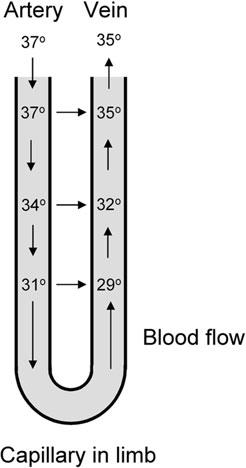
\includegraphics[width=0.35\textwidth]{618.png}
  \caption{Ejemplo de flujo de calor a contracorriente desde una arteria hacia una vena cercana. Sin este flujo, la caída de temperatura a lo largo de la arteria sería aún mayor en condiciones de frío porque habría más flujo de calor hacia el entorno. Todas las temperaturas están en $^\circ$C. Véase también la Fig. 6.19a (basado en \cite{69}).}
  \label{fig:618}
\end{SCfigure}



Si las arterias que fluyen hacia una parte del cuerpo, como una mano o un pie, están físicamente separadas de las venas que devuelven la sangre al corazón, la transferencia de calor de arterias a venas es mínima. Si, en cambio, están muy próximas entre sí, puede producirse una transferencia de calor sustancial desde la sangre más caliente que fluye por las arterias hacia la sangre más fría que fluye por las venas. (La sangre venosa es más fría debido a la pérdida de calor hacia los tejidos locales, que pueden estar mucho más fríos que el núcleo). Esto se denomina intercambio de calor a contracorriente, y se muestra en la Fig. 6.18 \cite{69}. Reduce la pérdida de calor total en la parte del cuerpo —especialmente en las extremidades y las regiones superficiales— y, por tanto, reduce la pérdida de calor total en la sangre y el cuerpo, porque disminuye la diferencia de temperatura entre la sangre en la parte del cuerpo y el tejido (y localmente, fuera del cuerpo). Como parte de su sistema de control de temperatura (Cap. 13), el cuerpo puede decidir si minimizar la pérdida de calor, utilizando el enfriamiento a contracorriente, o maximizarla, desviando más flujo sanguíneo hacia zonas más próximas a la piel. El intercambio de calor a contracorriente se modela en el Problema 6.114.

\begin{figure}[htbp]
  \centering
  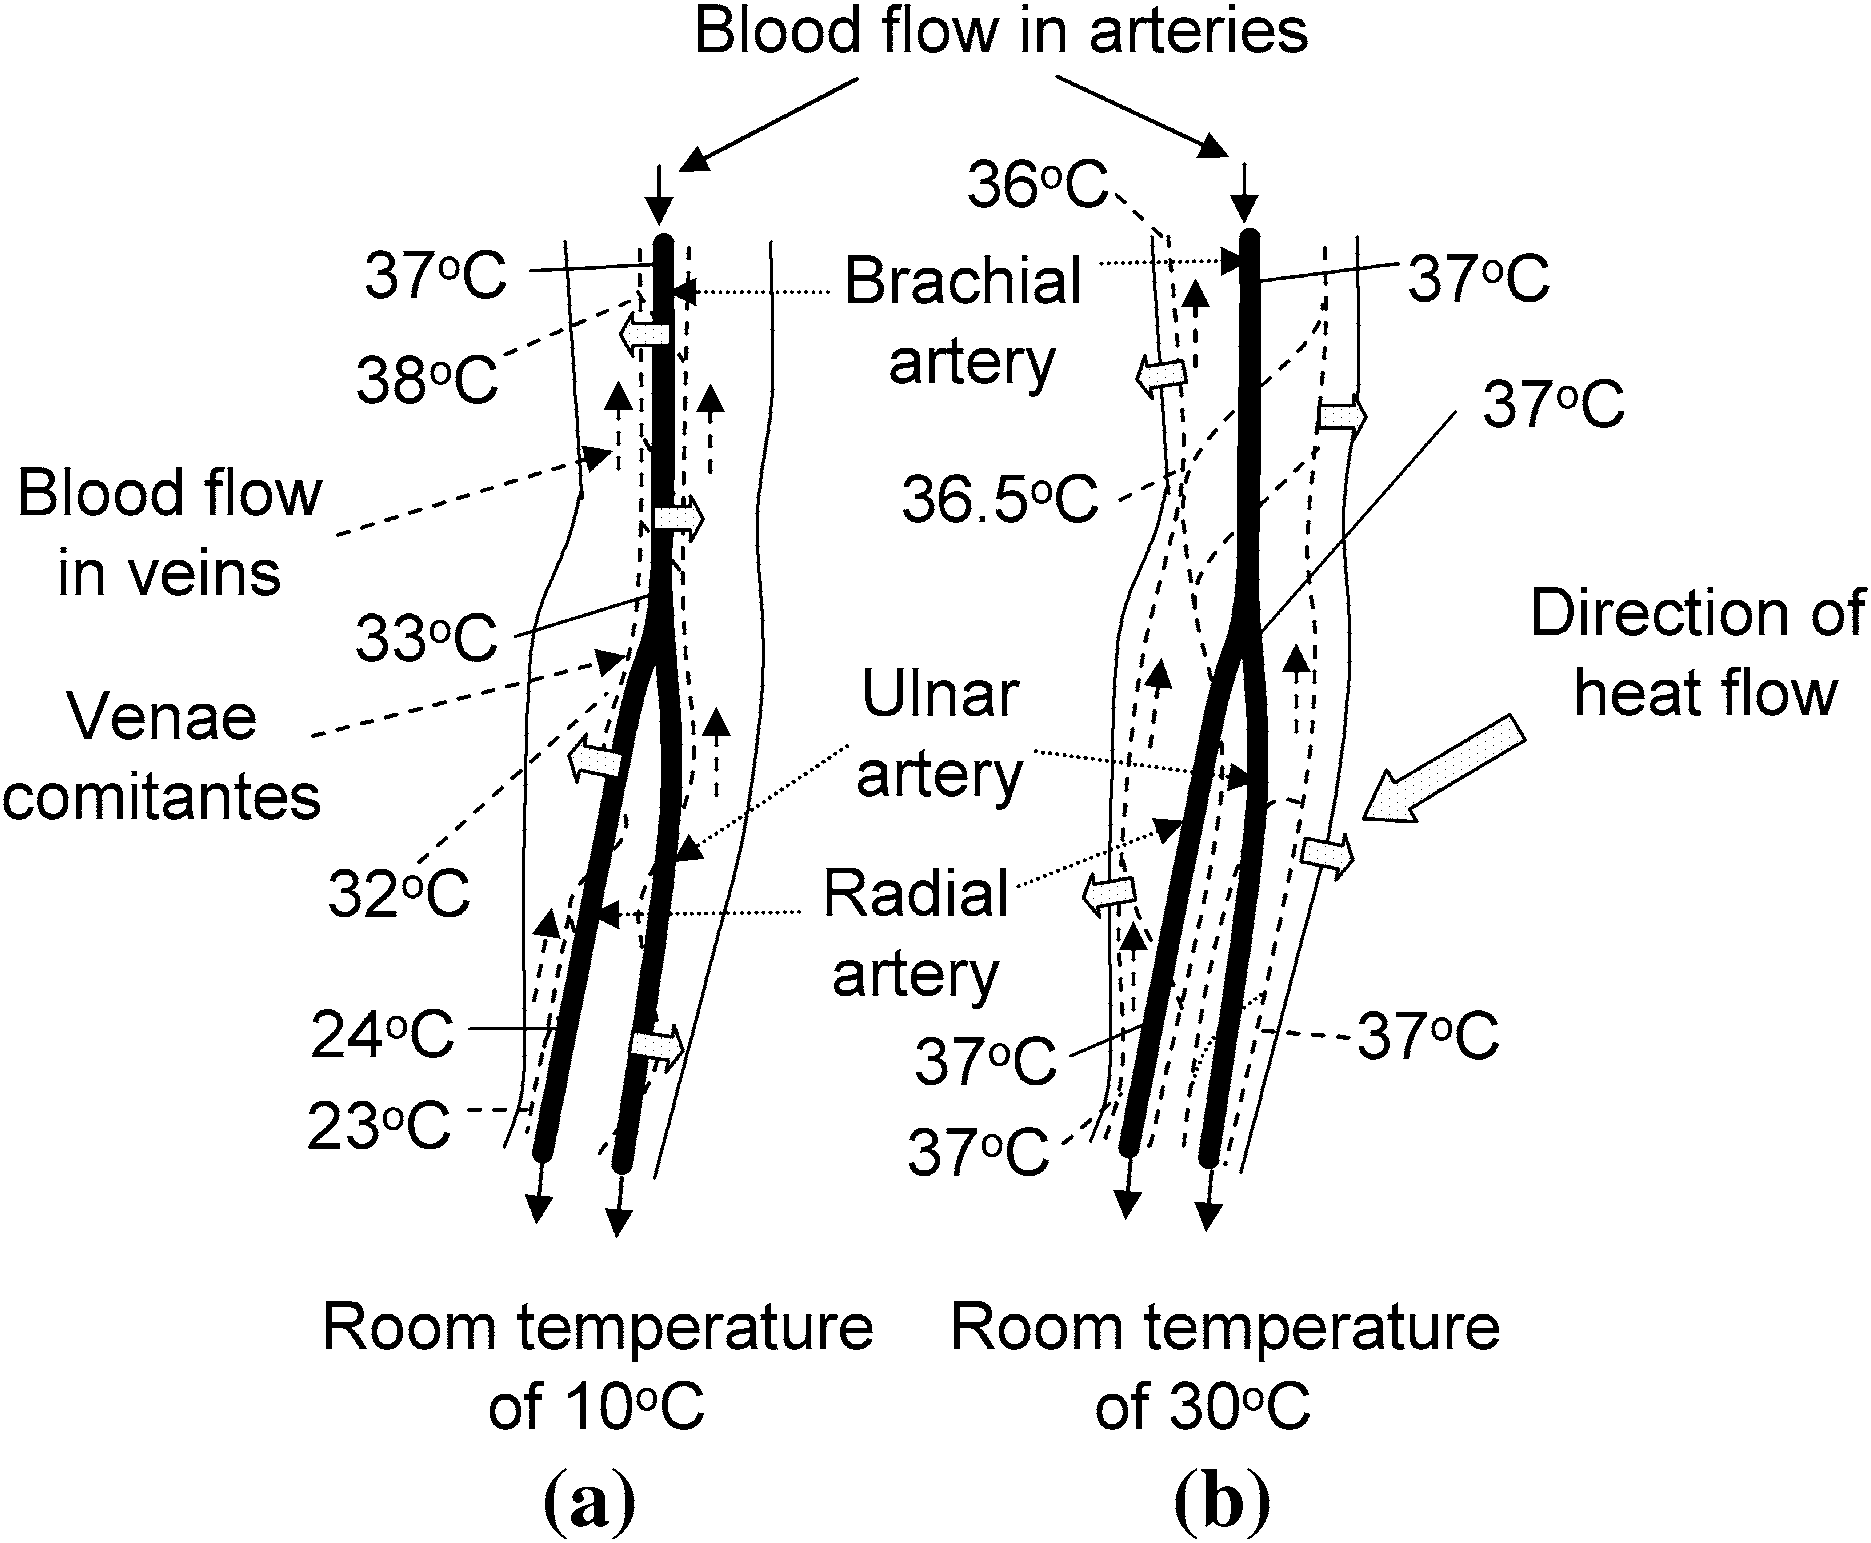
\includegraphics[width=0.7\textwidth]{619.png}
  \caption{Intercambio de calor a contracorriente en el brazo (derecho) para la sangre que fluye por la arteria braquial en (a). A temperaturas de habitación más altas ($30\ ^\circ$C) en (b) y durante el ejercicio, el retorno venoso fluye por vasos superficiales para permitir la pérdida de calor hacia la habitación. A la temperatura más baja ($10\ ^\circ$C) en (a), esta vía de retorno se desplaza a las venas profundas, lo que ayuda a retener el calor de dos formas: el calor de las arterias se transfiere a la sangre venosa antes de perderse hacia la habitación (intercambio de calor a contracorriente, Fig. 6.18), y se pierde poco calor hacia la habitación desde estas venas porque son profundas. Nótese que en el antebrazo inferior la temperatura en las venas comitantes es $1\ ^\circ$C más baja que en la arteria. Las venas comitantes son las venas que acompañan a las arterias en las extremidades. Se utilizan diferentes tipos de flechas para denotar el flujo sanguíneo en arterias (continua, estrecha), el flujo sanguíneo en venas (discontinua, estrecha) y el flujo de calor (ancha, gris) (basado en \cite{16,49}).}
  \label{fig:619}
\end{figure}



La Figura 6.19 muestra cómo ocurre esto en el antebrazo a través de dos conjuntos diferentes de venas. Si hace frío en la superficie del cuerpo, la sangre regresa al corazón a través de venas que están muy próximas a las arterias, de modo que la pérdida de calor se minimiza mediante el intercambio de calor a contracorriente. Dado que esto minimiza el calentamiento de las manos, es una de las formas de obtener manos excesivamente frías.

Si hace calor, el flujo sanguíneo cerca de la superficie y la transferencia de calor y el enfriamiento se maximizan. La sangre se dirige a estas venas «internas» y «externas» mediante músculos vasodilatadores y vasoconstrictores que rodean las venas apropiadas (para dilatarlas y contraerlas, respectivamente), controlados por el sensor de temperatura y el sistema de regulación de la temperatura (Cap. 12).

El intercambio de calor a contraflujo también se utiliza para regular la temperatura de los testículos. Estos se mantienen fuera del núcleo del cuerpo porque la fertilidad mejora a unos pocos grados por debajo de la temperatura central. Antes de que la sangre entre en la región de los testículos, suele experimentar un intercambio de calor a contraflujo para que entre sangre más fría en esta región. Esto evita un calentamiento excesivo de los testículos por la sangre caliente, así como la pérdida excesiva de calor corporal desde esta región «térmicamente» expuesta.

Un mecanismo multiplicador a contraflujo también es utilizado por el cuerpo en la difusión en el riñón para superar grandes gradientes de concentración \cite{69,95}.

\paragraph*{Conducción}

Como se muestra en (6.6), el flujo de calor durante la conducción térmica es el producto de la conductividad térmica $K$ y el gradiente de temperatura

\begin{equation}
-\frac{1}{A}\left(\frac{dQ}{dt}\right) = K\frac{dT}{dx} \sim K\frac{\Delta T}{\Delta x}.
\label{eq:668}
\end{equation}
Para una distancia bien definida $d = \Delta x$ entre dos regiones de temperatura diferente pero uniforme, por ejemplo debida al grosor de la ropa o a una capa límite de aire, podemos definir un coeficiente de transferencia de calor por unidad de área $h_t = K/d$ y

\begin{equation}
-\frac{1}{A}\left(\frac{dQ}{dt}\right) = h_t \Delta T,
\label{eq:669}
\end{equation}
como en (6.7). Esto tiene una forma similar a la de la pérdida de calor por radiación (neta) (6.53) y la convección forzada (6.59).

Determinemos cuánto calor pierde una persona cuando mete la mano y el antebrazo en agua muy fría ($4\ ^\circ$C) durante 2 min \cite{2}. Su mano y antebrazo pueden modelarse como un cilindro de longitud $L = 30\text{ cm}$ y radio promedio de $3\text{ cm}$. Supongamos que el cuerpo tiene una capa de grasa de $\Delta r = 3\text{ mm}$ de grosor con conductividad térmica $K = 0{,}2\text{ W/m-}^\circ\text{C}$ que separa el núcleo cilíndrico (de radio $r = 2{,}7\text{ cm}$, a $37\ ^\circ$C) del agua fría. El área de contacto entre el brazo y el agua es $A = 2\pi r L$. Usando (6.68) modificada para cilindros (reemplazando $\Delta x$ por $r\ln(1 + \Delta r/r)$, como se indicó antes), la tasa a la que el calor abandona el brazo es $(2\pi r L)(K \Delta T)/(r\ln(1 + \Delta r/r)) \simeq (2\pi r L K \Delta T)/(\Delta r)$. La expresión exacta da $118\text{ W}$, mientras que la aproximación da $112\text{ W}$. En 2 min, el cuerpo pierde $(118\text{ W})(120\text{ s}) = 14\,200\text{ J}$ o $3{,}4\text{ kcal}$.

El aislamiento $I$ puede definirse formalmente como $I = 1/h_t = d/K$. A veces se expresa en términos del valor de ropa o Clo, donde $1\text{ Clo}$ es el aislamiento para un hombre con un traje normal sin guantes o con guantes ligeros, que lleva zapatos de cuero y calcetines ligeros \cite{10,22}. Un aislamiento de $1\text{ Clo} = 0{,}155\text{ m}^2\text{-}^\circ\text{C/W}$ ($= 0{,}88\text{ ft}^2\text{-}^\circ\text{F/BTU}$). Una persona desnuda tiene $0\text{ Clo}$ de aislamiento. Un conjunto de trabajo ligero (calzoncillos, calcetines de lana, camisa de trabajo de algodón —con la parte inferior de la camisa por fuera y el cuello abierto— y pantalones de trabajo) corresponde a $0{,}6\text{ Clo}$. Un traje ligero típico tiene entre $0{,}7$ y $1{,}0\text{ Clo}$ del aislamiento, mientras que un traje de negocios pesado tiene $1{,}2\text{ Clo}$. Un traje para clima polar hecho de lana de pelo grueso tiene entre $3$ y $4\text{ Clo}$. Los valores típicos de aislamiento se indican en la Tabla 6.44. El aislamiento que proporciona la ropa humana es de aproximadamente $0{,}25\ ^\circ\text{C-m}^2/\text{W}$ por cm de grosor de ropa. La conductividad térmica de varios tejidos corporales se indica en la Tabla 6.36 y la de materiales comunes en la Tabla 6.37.

\subsubsection*{Pérdida de calor por evaporación del agua: sudoración y respiración}

La cantidad de calor necesaria para evaporar 1 L de agua es de $540\text{ kcal}$ (cerca de su punto de ebullición); este es el calor de vaporización. Cuando sudamos hay pérdida de calor solo si se permite que el agua se evapore. (Limpiarse el sudor no lo enfriará). Esto normalmente representa una pérdida de $\sim 7\text{ kcal/h}$.

\begin{table}[htbp]
\centering
\caption{El aislamiento de pelajes de animales, tejidos, componentes corporales y otros materiales, en unidades de m$^2$-$^\circ$C/W por cm de aislamiento}
\label{tab:644}
\small
\begin{tabularx}{0.85\textwidth}{X >{\centering\arraybackslash}X}
\toprule
\textbf{Material} & \textbf{Aislamiento por cm} \\
\midrule
Pelaje de ganado & 0{,}07--0{,}10 \\
Pelaje de oveja & 0{,}13--0{,}24 \\
Pelaje de perro husky & 0{,}24 \\
Pelaje de cerdo & 0{,}04 \\
Lana & 0{,}29 \\
Plumón de ganso & 0{,}38 \\
Ropa humana (promedio) & 0{,}25 \\
Aire & 0{,}36 / 0{,}39 \\
Músculo, hueso & 0{,}01 / 0{,}024 \\
Grasa corporal & 0{,}01 / 0{,}05 \\
Agua & 0{,}01 / 0{,}017 \\
Hielo & 0{,}01 / 0{,}004 \\
Madera típica\textsuperscript{a} & 0{,}01 / 0{,}062 \\
\bottomrule
\end{tabularx}
\begin{flushleft}
    \small $h_t$ es $1/(\text{aislamiento por cm} \times \text{el espesor en cm})$. La conductividad térmica $K$ es $1/(\text{aislamiento por cm})$ o $0{,}01 \times$ este valor cuando se expresa en unidades de W/m-$^\circ$C.\\
    \textsuperscript{a}La madera de balsa es mayor; la madera verde es menor.\\
    Utilizando datos de \cite{2,11}; también véase \cite{22}
\end{flushleft}
\end{table}

Normalmente inspiramos aire que está más frío que la temperatura corporal. Este se calienta y luego se exhala: esto también es una fuente de enfriamiento corporal. Además, inspiramos aire relativamente seco y exhalamos aire saturado con vapor de agua. Debido a que este vapor de agua se forma por la evaporación de agua líquida, esta es otra fuente más de enfriamiento. La pérdida de calor respiratoria debida a los pulmones se puede describir por
\begin{equation}
-\left(\frac{dQ}{dt}\right)_l = \rho_{\text{air}} c_{p, \text{air}} (T_{\text{exp}} - T_{\text{insp}}) \frac{dV_{\text{air}}}{dt} + H_{\text{evap, water}} (\rho_{\text{exp, water}} - \rho_{\text{insp, water}}) \frac{dV_{\text{air}}}{dt},
\label{eq:670}
\end{equation}
donde $\rho$ es la densidad de masa (del aire o del vapor de agua espirado o inspirado), $c_{p, \text{air}}$ es el calor específico del aire ($2{,}4 \times 10^{-4}\text{ kcal/g-}^\circ\text{C}$), $T$ es la temperatura del aire espirado o inspirado, $dV/dt$ es la tasa de inhalación de aire y $H_{\text{evap, water}}$ es el calor de evaporación del agua ($0{,}54\text{ kcal/g}$). El primer término da cuenta del enfriamiento corporal debido al calentamiento del aire inspirado antes de la espiración (exhalación) y el segundo término da cuenta del enfriamiento corporal por la evaporación de agua en los pulmones, la cual incrementa el contenido de agua del aire inspirado antes de la espiración.

Cuando hace calor, ¿por qué se siente aún más caliente que la temperatura ambiente cuando hay humedad? La humedad disminuye la tasa de pérdida de calor del cuerpo al reducir el flujo de calor desde el cuerpo hacia el aire, disminuyendo la evaporación del sudor (porque la presión de vapor de agua en el aire reduce la diferencia entre la presión de vapor sobre el sudor y en el aire) y disminuyendo la tasa de pérdida de calor respiratoria debido al último término en (\ref{eq:670}). El índice de calor describe qué tan caliente se siente realmente a una temperatura y humedad dadas \cite{96,97}. Por ejemplo, cuando hace $90\ ^\circ\text{F}$ ($32\ ^\circ\text{C}$), se siente como si hiciera $95\ ^\circ\text{F}$ ($35\ ^\circ\text{C}$) cuando la humedad relativa es del $50\%$, $109\ ^\circ\text{F}$ ($43\ ^\circ\text{C}$) cuando es del $75\%$ y $132\ ^\circ\text{F}$ ($56\ ^\circ\text{C}$) when the relative humidity is 100\% (cuando es del $100\%$). (La humedad relativa es la presión de vapor real de agua en el aire dividida por la presión de vapor de equilibrio del agua (en contacto con agua líquida), a la misma temperatura. Normalmente se expresa en porcentaje). La probabilidad de trastornos por calor, como la insolación y el golpe de calor, se caracteriza por advertencias tales como «precaución» para valores del índice de calor de $80\text{--}90\ ^\circ\text{F}$ ($27\text{--}32\ ^\circ\text{C}$), «precaución extrema» de $90$ a $105\ ^\circ\text{F}$ ($32$ a $41\ ^\circ\text{C}$), «peligro» de $105$ a $129\ ^\circ\text{F}$ ($41$ a $54\ ^\circ\text{C}$) y «peligro extremo» por encima de $130\ ^\circ\text{F}$ ($54\ ^\circ\text{C}$). El índice de calor se explora más en los Problemas 6.120--6.123.

El efecto de la humedad del aire también se puede evaluar considerando tres «temperaturas»: la temperatura habitual de bulbo seco, la temperatura de bulbo húmedo y el punto de rocío. La temperatura de bulbo húmedo de un objeto es la temperatura a la que se enfriaría el objeto, al suministrar el calor de vaporización, de modo que localmente habría una humedad relativa del $100\%$. El termómetro de bulbo húmedo es un termómetro de bulbo seco cubierto con un material empapado en agua, por lo que indica el efecto máximo del enfriamiento evaporativo al nivel de humedad absoluta. El punto de rocío es la temperatura a la que comienza la condensación (humedad relativa del $100\%$) al nivel de humedad absoluta. Para una humedad relativa del $100\%$, las tres temperaturas son iguales; a medida que esta disminuye, la temperatura de bulbo húmedo disminuye y el punto de rocío disminuye aún más rápido. La temperatura de bulbo húmedo proporciona una indicación de la regulación de la temperatura corporal debido al enfriamiento evaporativo. Para temperaturas de bulbo húmedo de $\approx 95\ ^\circ\text{F}$ ($35\ ^\circ\text{C}$) y superiores, el cuerpo no puede enfriarse lo suficiente únicamente mediante el enfriamiento evaporativo.

Los humanos podemos correr largas distancias en parte porque podemos perder calor sudando, pudiendo evaporar más de un litro de agua por hora. Tenemos entre $3$ y $10\text{ millones}$ de glándulas sudoríparas en todo el cuerpo. Sin ellas, tendríamos que depender del jadeo, como hacen los animales con pelaje, quienes poseen glándulas sudoríparas para enfriamiento solo en regiones desprovistas de pelo, como en las almohadillas de las patas en el caso de los perros \cite{44,56,91}.

\section{Temperatura corporal}

La temperatura corporal central normal está en el rango de $36{,}5\text{--}37{,}5\ ^\circ\text{C}$ ($97{,}7\text{--}99{,}5\ ^\circ\text{F}$); para un individuo dado, la temperatura central generalmente aumenta durante las horas de vigilia en $0{,}5\ ^\circ\text{C}$ ($\sim 0{,}9\ ^\circ\text{F}$). La anestesia disminuye la temperatura corporal central en $\sim 1\ ^\circ\text{C}$, probablemente porque los anestésicos interfieren con la forma en que el cuerpo regula la temperatura; también puede provocar variaciones de temperatura de varios grados a lo largo de las superficies de las extremidades \cite{37}. Las temperaturas medidas en el recto son $0{,}4\ ^\circ\text{C}$ ($\sim 0{,}7\ ^\circ\text{F}$) más altas que las medidas en la boca \cite{59}.

\begin{figure}[htbp]
  \centering
  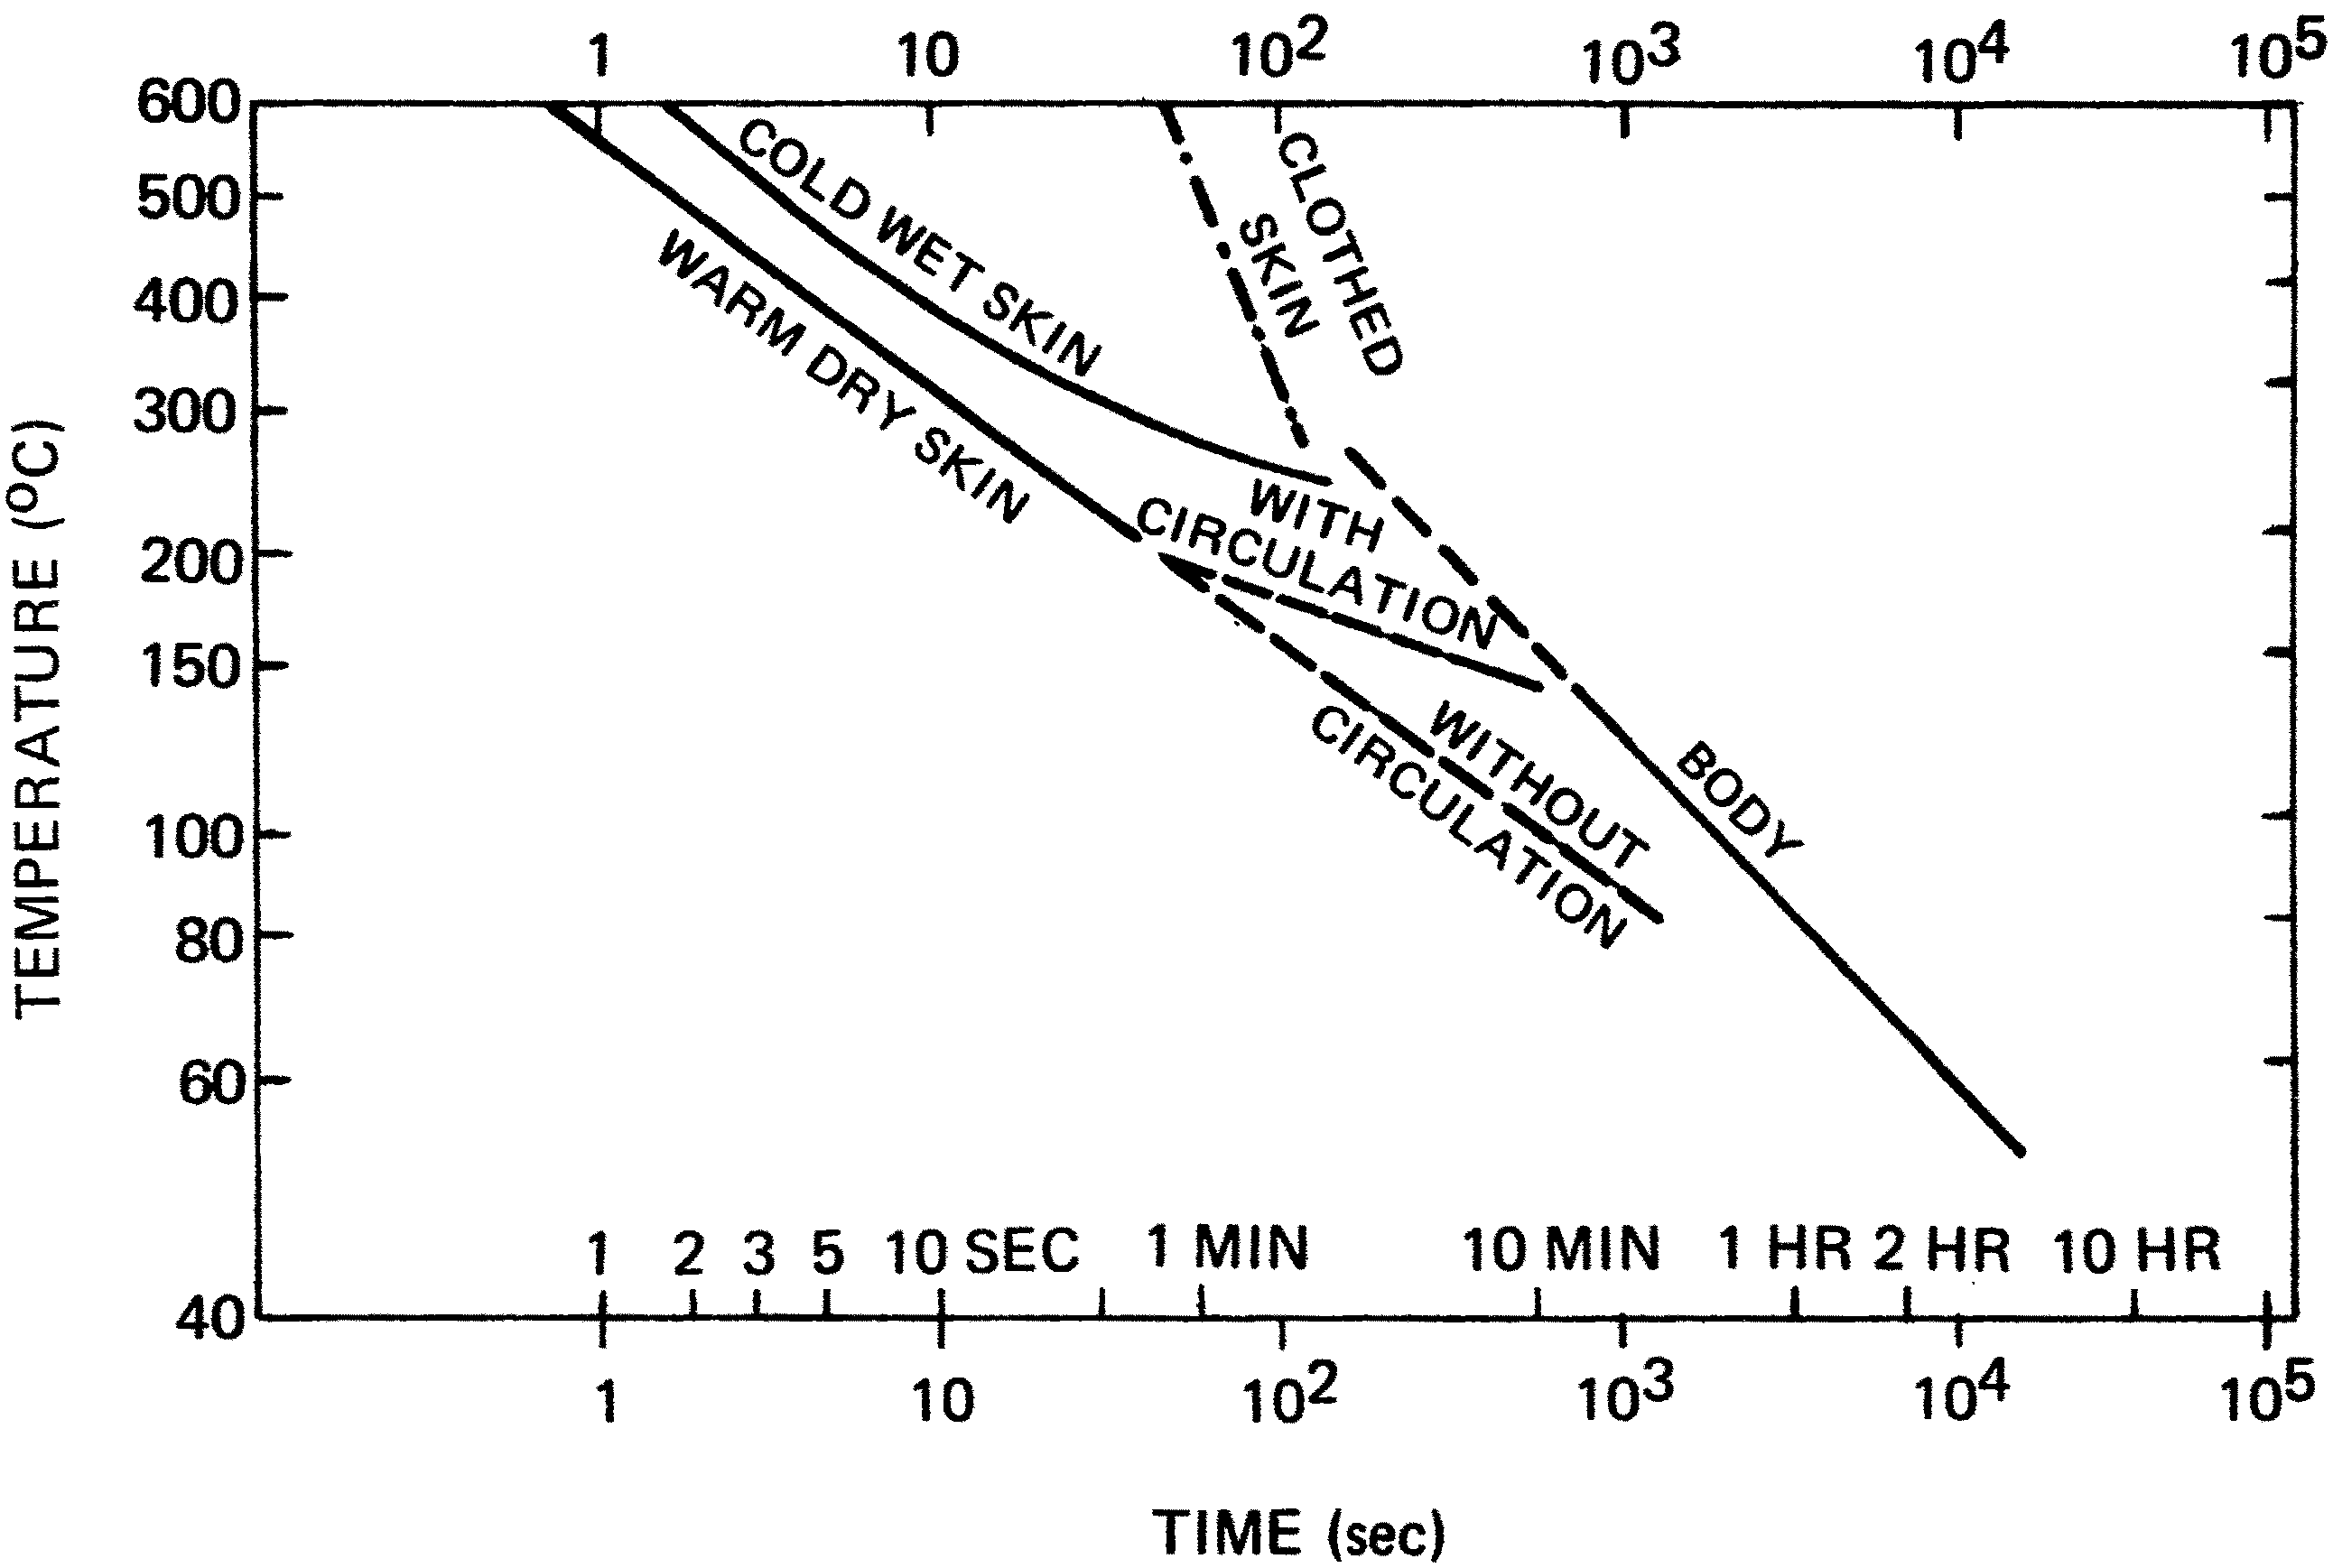
\includegraphics[width=0.7\textwidth]{620.png}
  \caption{Control corporal de la temperatura central durante varias horas con grandes variaciones en la temperatura ambiental local, para aire seco. La temperatura corporal normal de $98{,}6\ ^\circ\text{F}$ ($37\ ^\circ\text{C}$) se mantiene para temperaturas atmosféricas desde $\sim 70$ hasta $130\ ^\circ\text{F}$ ($\sim 21$ a $54\ ^\circ\text{C}$). La forma exacta de esta curva depende del entorno: humedad, movimiento del aire, radiación térmica hacia el cuerpo, etc. (basado en \cite{45}).}
  \label{fig:620}
\end{figure}

\begin{figure}[htbp]
  \centering
  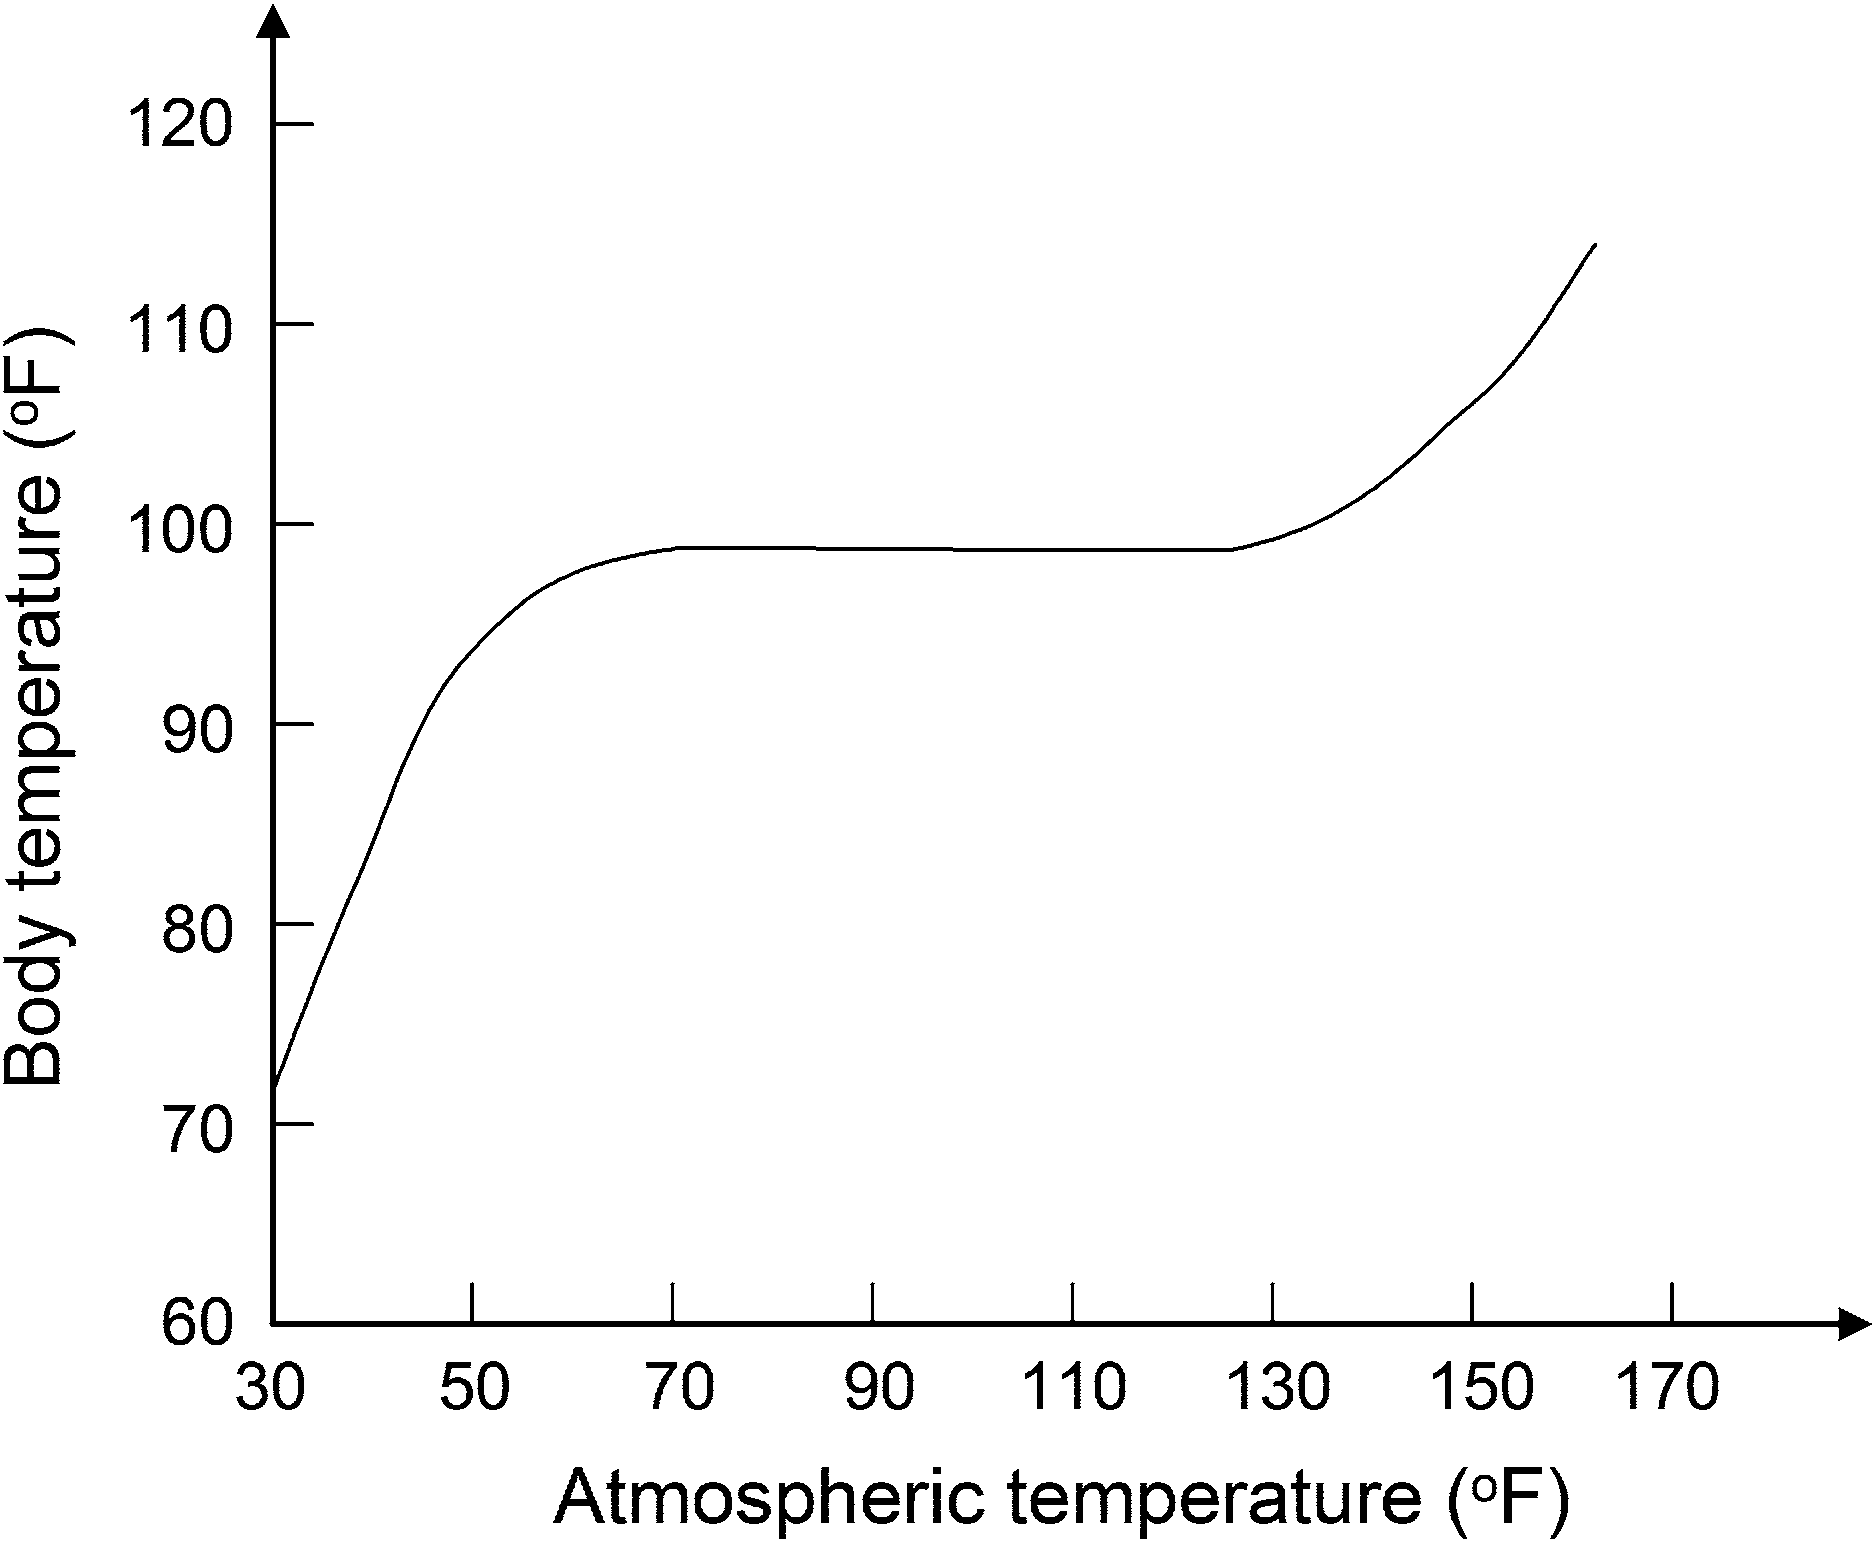
\includegraphics[width=0.7\textwidth]{621.png}
  \caption{Temperaturas elevadas máximas tolerables (del aire) en función de los tiempos de exposición, para diferentes condiciones corporales. Las condiciones tolerables están por debajo de las líneas para cada condición de la piel y para el cuerpo, y las condiciones intolerables están por encima de ellas (de \cite{10}).}
  \label{fig:621}
\end{figure}

\begin{figure}[htbp]
  \centering
  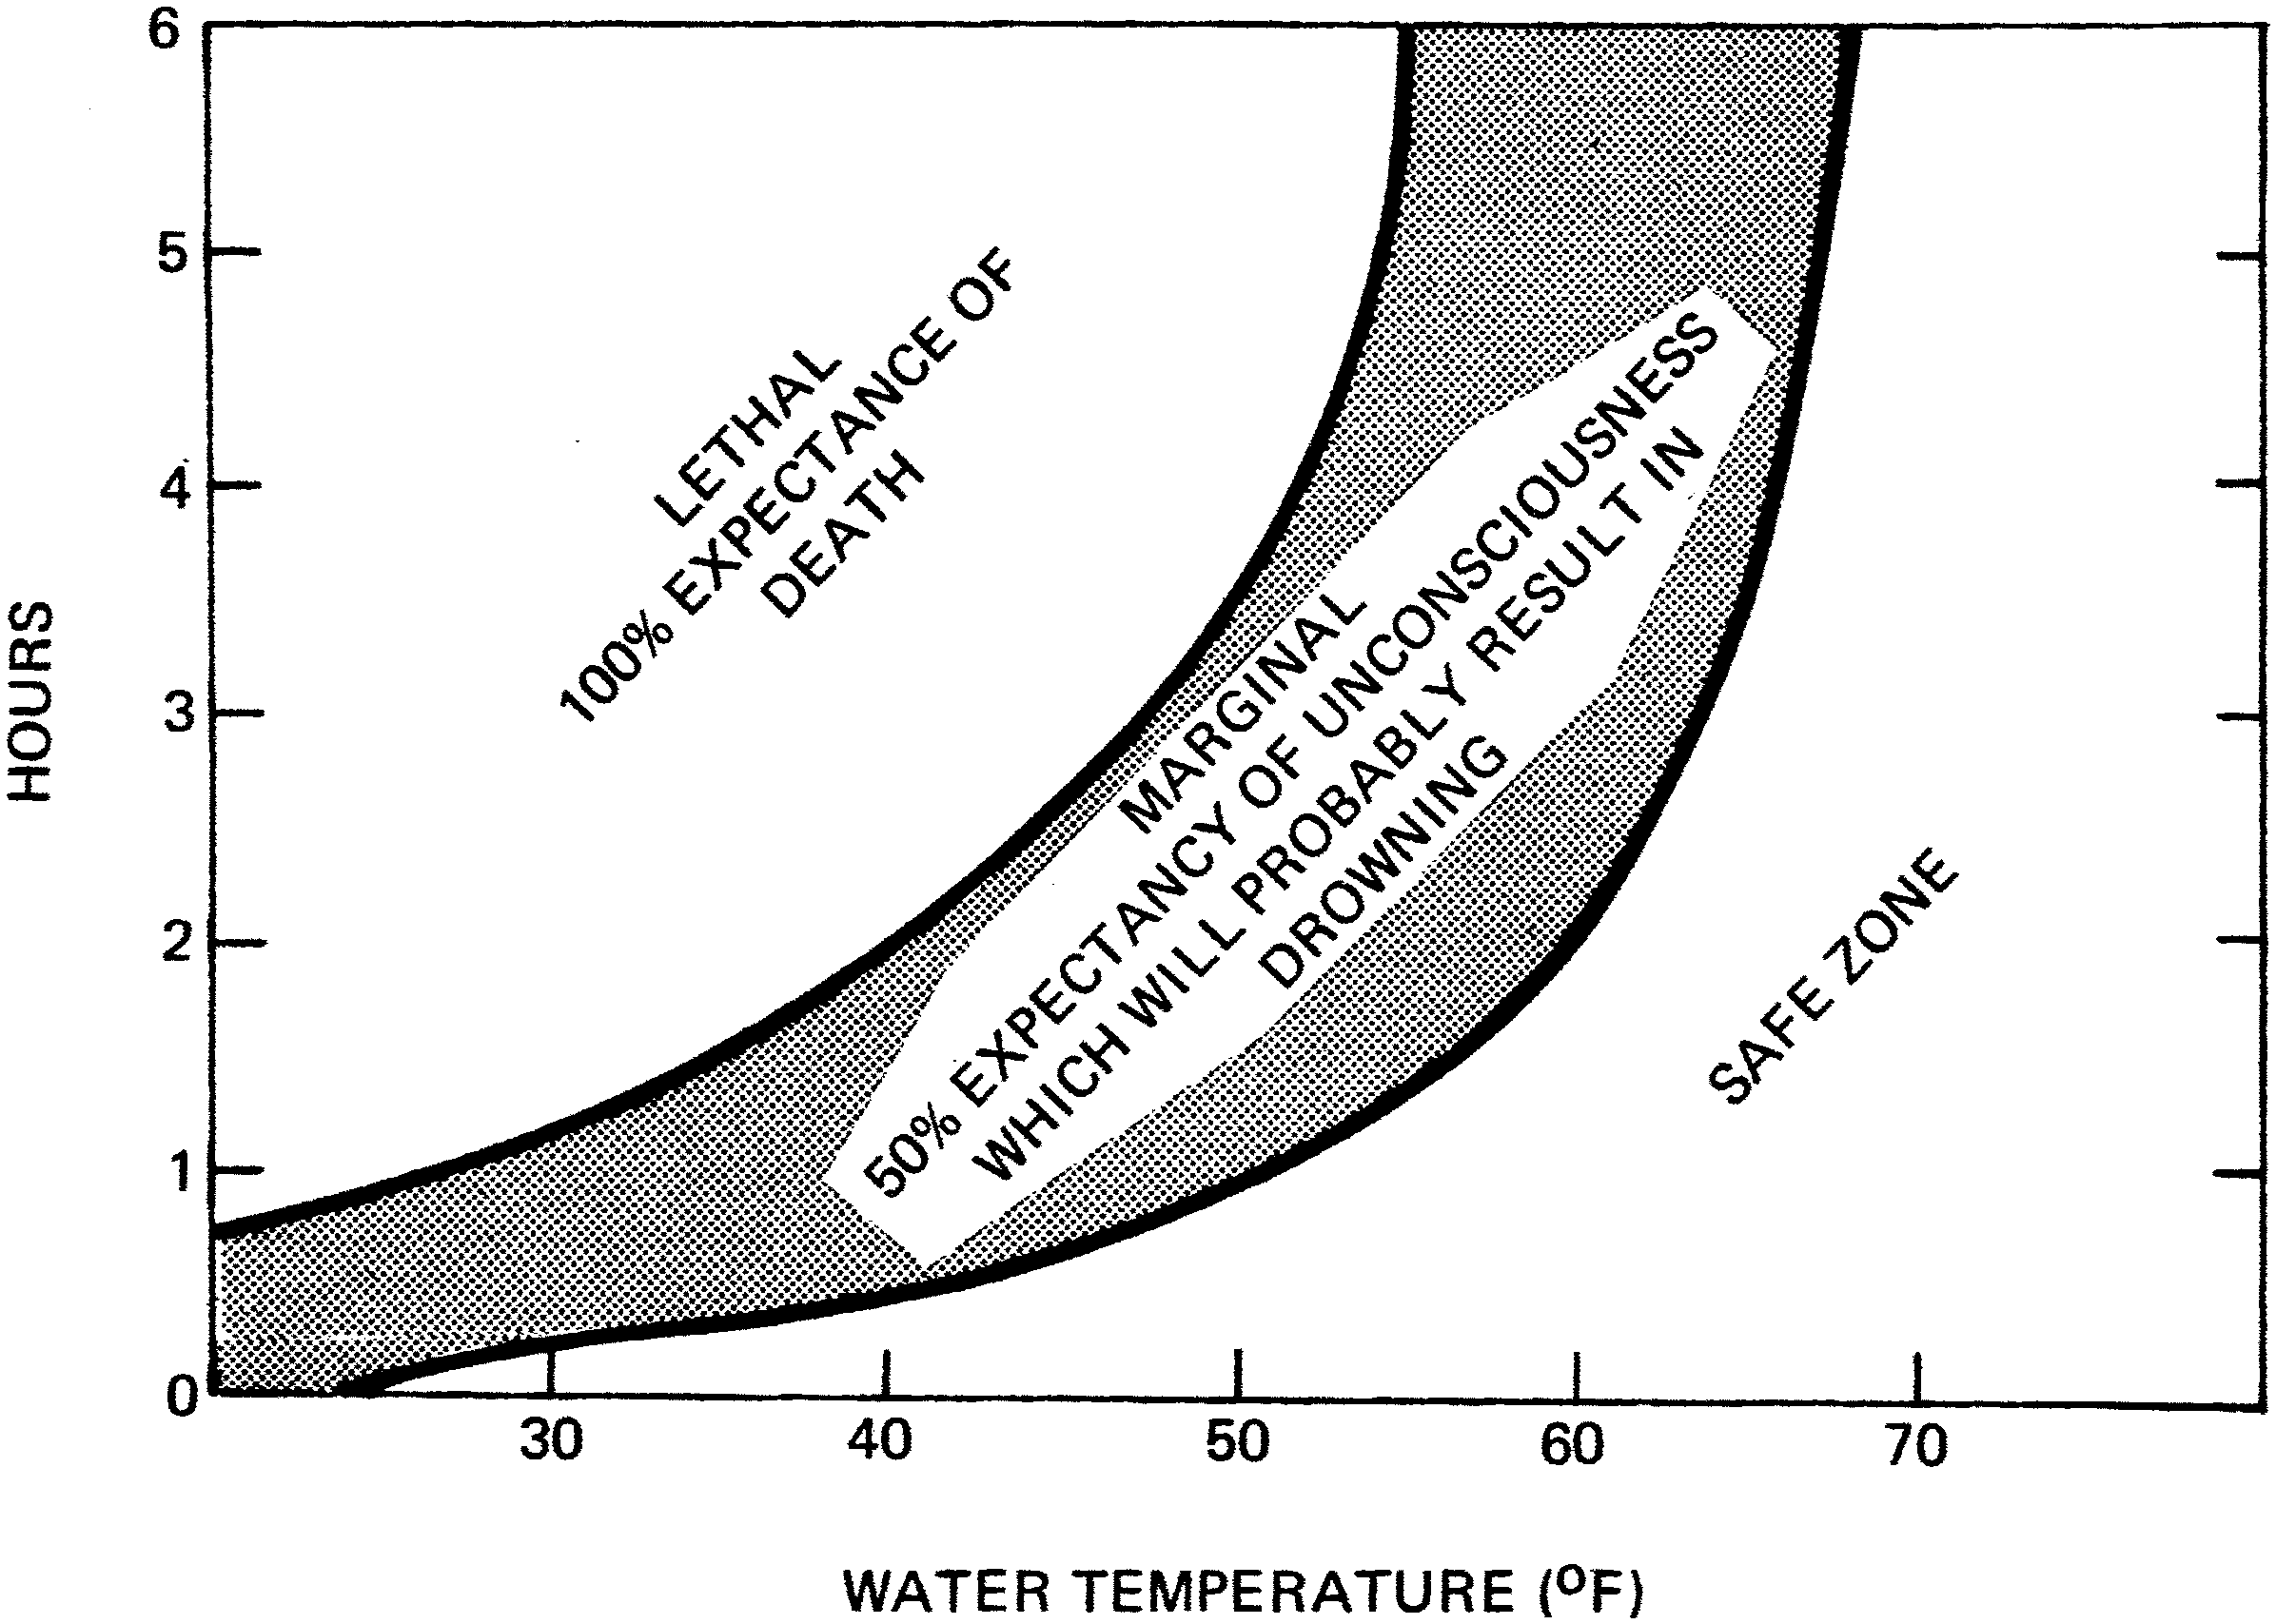
\includegraphics[width=0.7\textwidth]{622.png}
  \caption{Esperanza de vida de una persona sin traje de exposición en agua fría para diferentes tiempos (de \cite{10}).}
  \label{fig:622}
\end{figure}

\begin{figure}[htbp]
  \centering
  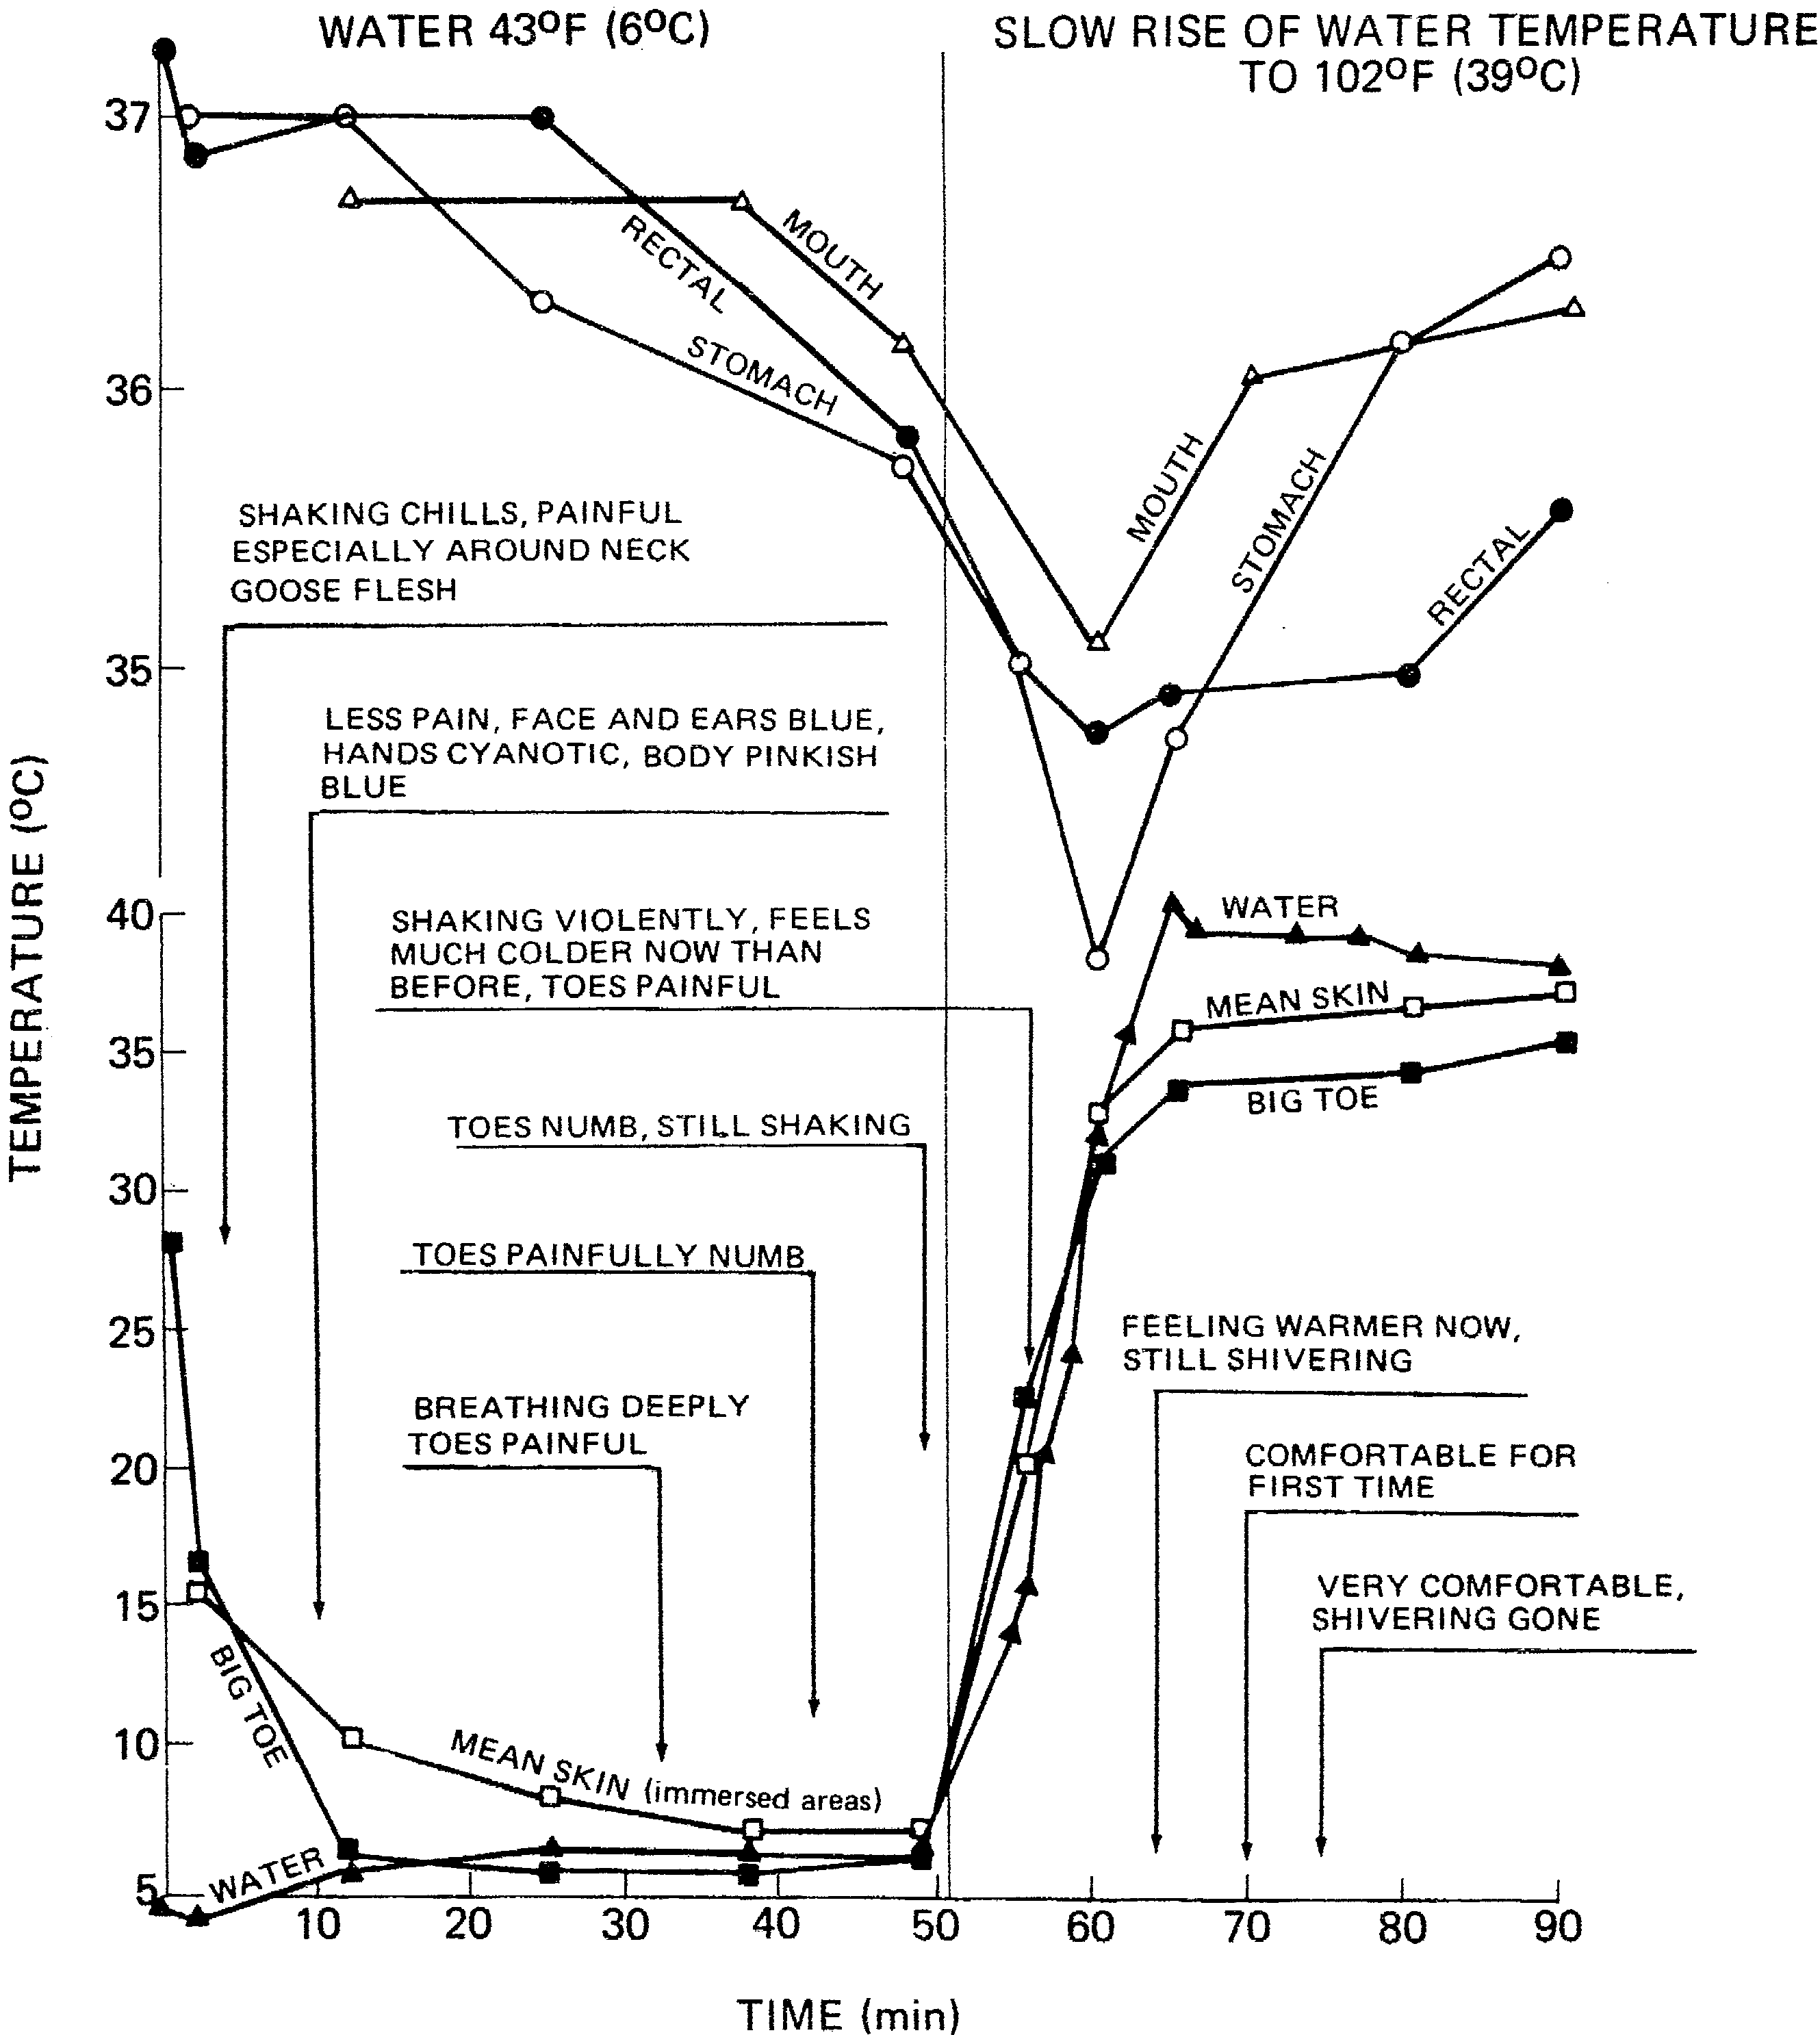
\includegraphics[width=0.55\textwidth]{623.png}
  \caption{Variación en la temperatura cutánea e interna cuando una persona se sumerge en agua a $6\ ^\circ\text{C}$ ($43\ ^\circ\text{F}$) durante $52\text{ min}$ y luego se calienta lentamente usando agua a $39\ ^\circ\text{C}$ (de \cite{10}).}
  \label{fig:623}
\end{figure}



El cuerpo es muy bueno controlando su temperatura. La Figura 6.20 muestra que el cuerpo desnudo puede mantener la temperatura central entre $97$ y $100\ ^\circ\text{F}$ ($36$ y $38\ ^\circ\text{C}$) durante varias horas con temperaturas ambientales que oscilan entre $70$ y $130\ ^\circ\text{F}$ ($21$ y $54\ ^\circ\text{C}$) en aire seco. Sin embargo, claramente tenemos límites. La Figura 6.21 muestra que podemos tolerar solo una exposición limitada al aire caliente, mientras que la Fig. 6.22 muestra que podemos sobrevivir solo a una exposición limitada al agua fría; en ambos casos, cuanto mayor sea la desviación de la temperatura respecto a la temperatura corporal normal, menor será el tiempo máximo de exposición posible antes de la muerte. La Figura 6.23 registra cómo disminuyen las temperaturas de la piel y del interior del cuerpo durante la exposición al agua fría, y cómo se recuperan cuando el cuerpo se coloca luego en agua tibia. ¿Cómo cambian las energéticas del cuerpo para mantener la temperatura normal y resistir los cambios que pueden ser inducidos por temperaturas ambientales extremas o por el ejercicio?

Cada uno de los modos de pérdida de calor corporal que hemos descrito es important para la regulación de la temperatura corporal. Se puede controlar la vía de convección cambiando de ropa. Algunos modos se controlan de forma involuntaria por el cuerpo, como el sudor y la respiración. ¿Qué sucede cuando la temperatura de la habitación supera la temperatura central y de la piel del cuerpo? El cuerpo entonces se calienta por radiación. La convección debe ser reevaluada. El aire exhalado ya no se calienta. ¿Qué sucede cuando se hace ejercicio y la tasa metabólica aumenta? El cuerpo tiene que responder de manera que aumente la tasa de pérdida de calor corporal. Todos estos modos de pérdida de calor son importantes. Un modelo cuantitativo de esta regulación se presenta en el Cap. 13, como parte de la discusión sobre la retroalimentación y el control en el cuerpo.

\begin{SCfigure}[0.9][htbp]
  \centering
  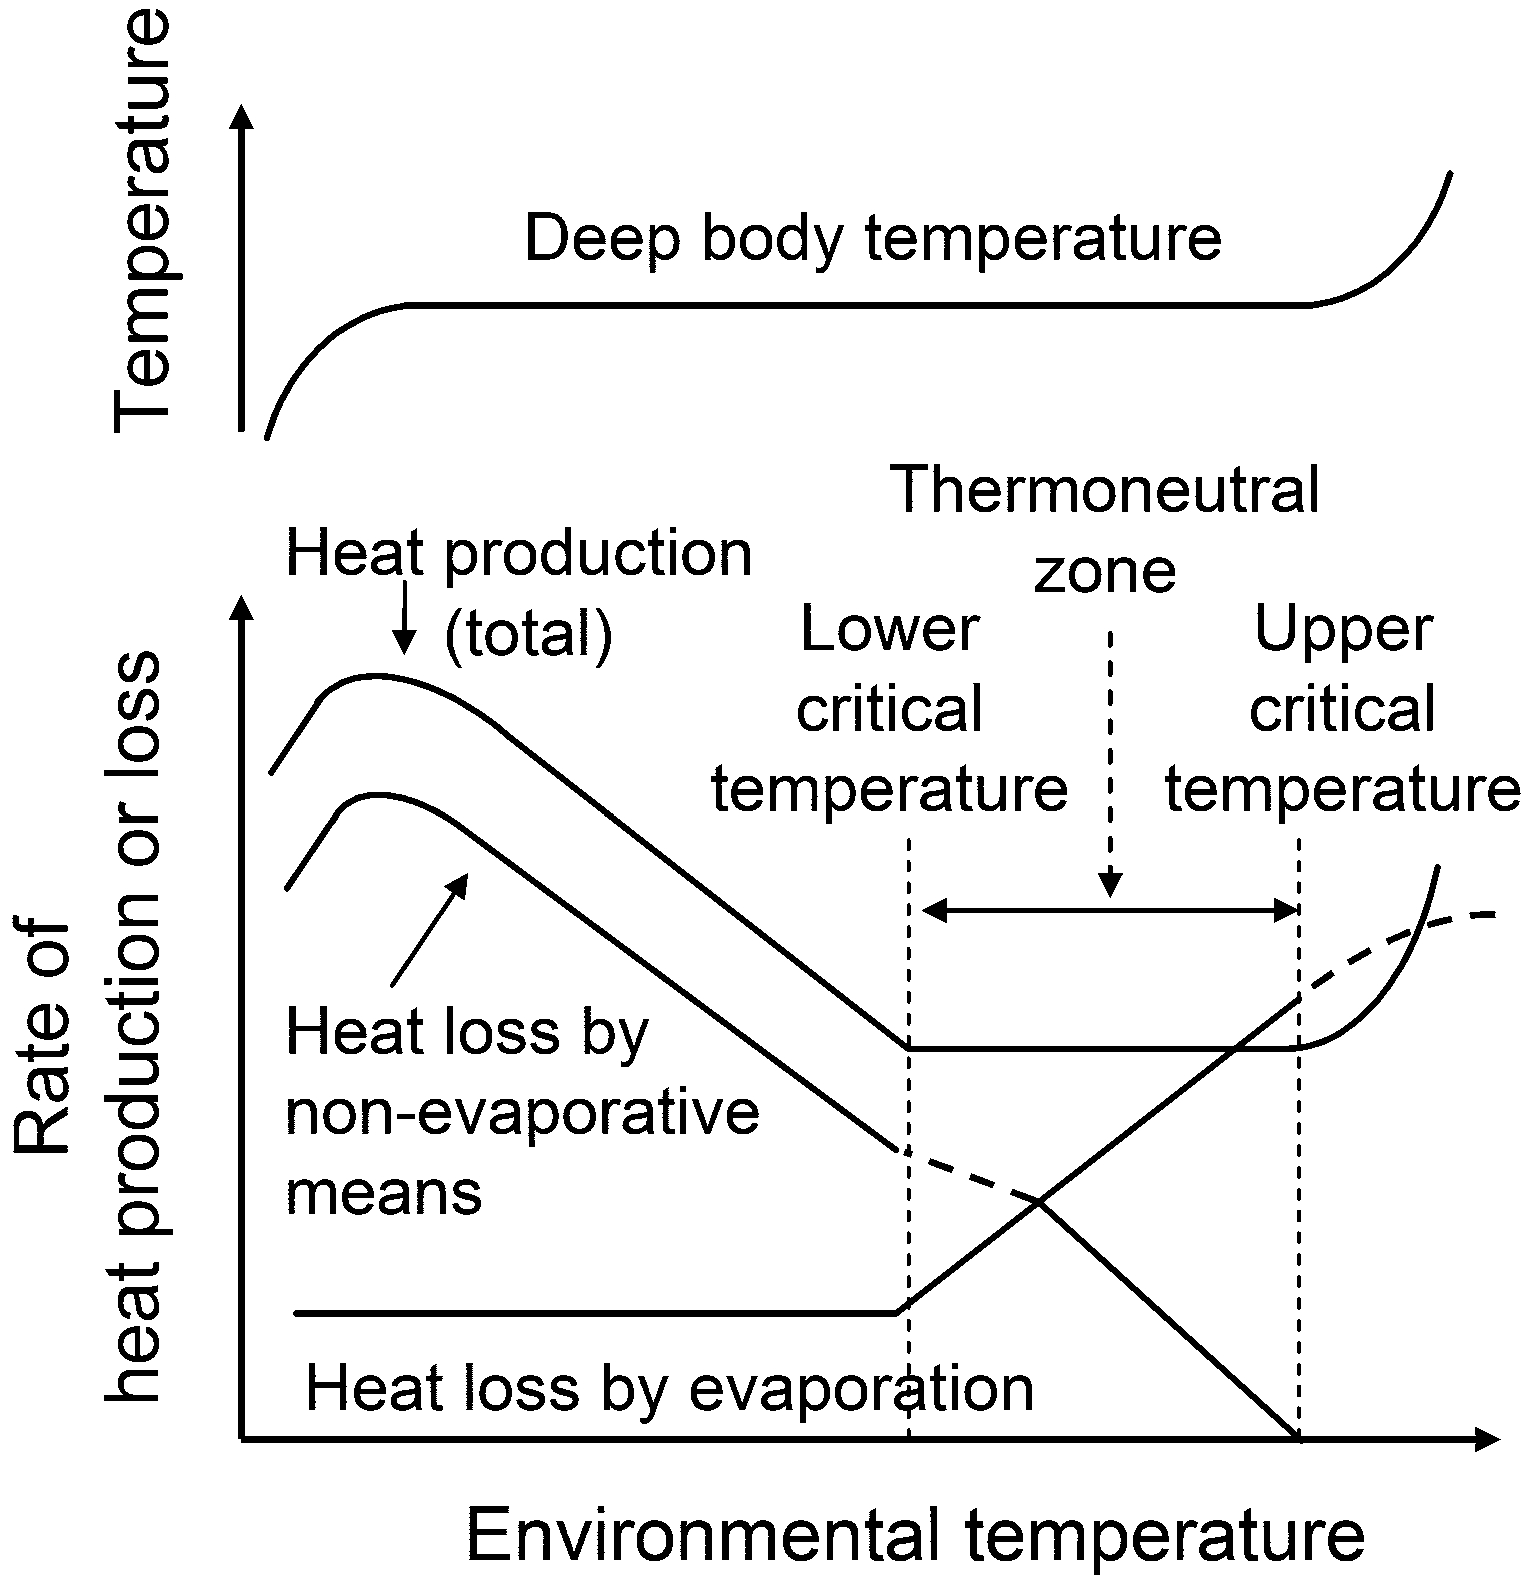
\includegraphics[width=0.5\textwidth]{624.png}
  \caption{Temperaturas críticas y relación entre la temperatura ambiental y la producción de calor en animales homeotermos (que son aquellos que poseen una temperatura corporal constante y relativamente alta, es decir, aves y mamíferos) (basado en \cite{11,72}).}
  \label{fig:624}
\end{SCfigure}



La producción de calor varía con la temperatura ambiental local, que llamamos $T_{\text{room}}$ anteriormente. Es alta a bajas temperaturas, luego disminuye con el aumento de la temperatura hasta $T_{\text{c}}$, se vuelve constante y luego en $T_{\text{h}}$ aumenta nuevamente, como se muestra en la Fig. 6.24. La temperatura crítica $T_{\text{c}}$ (o temperatura crítica inferior) es, por lo tanto, la temperatura ambiental a la cual la producción de calor comienza a aumentar cuando la temperatura ambiental cae. Es de $26\ ^\circ\text{C}$ para un hombre adulto desnudo y de $35\ ^\circ\text{C}$ para un bebé desnudo, asumiendo un movimiento de aire mínimo. De manera similar, la temperatura de aumento hipertérmico $T_{\text{h}}$ (o temperatura crítica superior) es la temperatura ambiental a la cual la producción de calor comienza a aumentar cuando la temperatura ambiental se incrementa. Entre $T_{\text{c}}$ y $T_{\text{h}}$ se encuentra la zona de metabolismo mínimo o zona termoneutral.

Por debajo de $T_{\text{c}}$, la pérdida de calor aumenta debido a vías no evaporativas, como la radiación y la convección. El aumento del metabolismo se debe a incrementos en la tensión muscular y al tiritar, que técnicamente es el movimiento visible del músculo subcutáneo. Esto aumenta a medida que se incrementa la diferencia entre la temperatura corporal y la ambiental, hasta que se alcanza el metabolismo de cumbre para esa temperatura ambiental. El metabolismo de cumbre es de aproximadamente $21 m_{\text{b}}^{0{,}75}$, en W con $m_{\text{b}}$ en kg, para el hombre (y generalmente alrededor de $25 m_{\text{b}}^{0{,}75}$ para la mayoría de los mamíferos). Esto es aproximadamente $7$ veces la tasa de metabolismo en ayuno o $2\text{--}3$ veces la tasa de gasto energético en el campo. (Sigue siendo mucho menor que las tasas metabólicas máximas que se pueden alcanzar durante el ciclismo, la carrera, etc.). A temperaturas más bajas, la temperatura corporal central no se puede mantener y se produce enfriamiento corporal e hipotermia. Por encima de $T_{\text{h}}$, la pérdida de calor está dominada por la evaporación.

La temperatura crítica se puede evaluar igualando la pérdida de calor y la producción de calor por el metabolismo. Durante el ejercicio, también deben considerarse el trabajo realizado y el calor almacenado o liberado por los tejidos. La temperatura corporal central se puede relacionar con la capacidad aeróbica máxima mediante
\begin{equation}
T_{\text{core}}\ (^\circ\text{C}) = 36{,}5 + 3{,}0 \times \frac{\text{consumo de oxígeno}}{\text{consumo máximo posible de oxígeno}},
\label{eq:671}
\end{equation}
debido a que las tasas de consumo de oxígeno son proporcionales a las tasas metabólicas. Además, el movimiento durante el ejercicio aumenta la pérdida de calor por convección. Un aumento en la temperatura corporal de $1\ ^\circ\text{C}$ incrementa la producción de calor en $\sim 13\%$. La producción de calor también es inducida por pirógenos, etc., y por traumatismos, fracturas óseas, quemaduras, etc.

La temperatura $T$ en (\ref{eq:635}) es la temperatura corporal promedio. La temperatura de la piel del cuerpo $T_{\text{skin}}$ ($34\ ^\circ\text{C} = 307\text{ K}$) suele ser menor que la del núcleo (rectal) $T_{\text{core}}$ ($37\ ^\circ\text{C} = 310\text{ K}$), que es la que se mide con un termómetro. La Tabla 6.45 presenta la temperatura normal de diferentes órganos corporales y vasos sanguíneos. La temperatura de los órganos internos puede diferir en $0{,}2\text{--}1{,}2\ ^\circ\text{C}$ y en $0{,}9\ ^\circ\text{C}$ en un órgano determinado bajo condiciones normales \cite{38}. Existen variaciones de temperatura de $1{,}4\ ^\circ\text{C}$ en el cerebro, siendo la corteza más fría que las regiones basales. La temperatura promedio del cuerpo es el promedio ponderado de las dos temperaturas, $T_{\text{av}} = (80 \pm 5\%) T_{\text{core}} + (20 \pm 5\%) T_{\text{skin}}$.

\begin{table}[htbp]
\centering
\caption{Temperaturas centrales dentro del cuerpo humano}
\label{tab:645}
\small
\begin{tabularx}{0.65\textwidth}{X >{\centering\arraybackslash}X}
\toprule
\textbf{Región corporal} & \textbf{Temperatura normal ($^\circ$C)} \\
\midrule
Piel & 32--35 \\
Escroto & 34{,}0 \\
Hígado & 36{,}4--36{,}8 \\
Cavidad oral & 36{,}5--36{,}6 \\
Vena cava superior & 36{,}65 \\
Esófago, pulmones & 36{,}75 \\
Corazón (ventrículo derecho) & 36{,}75 \\
Aorta, vena cava inferior & 36{,}75 \\
Arteria y vena pulmonar & 36{,}75 \\
Riñón & 36{,}85 \\
Médula espinal & 36{,}95 \\
Estómago, recto (media) & 37{,}0 \\
Recto (rango) & 36{,}2--37{,}8 \\
Cerebro, útero & 37{,}3 \\
\bottomrule
\end{tabularx}
\begin{flushleft}
    \small Utilizando datos de \cite{38}
\end{flushleft}
\end{table}

\begin{SCfigure}[0.9][htbp]
  \centering
  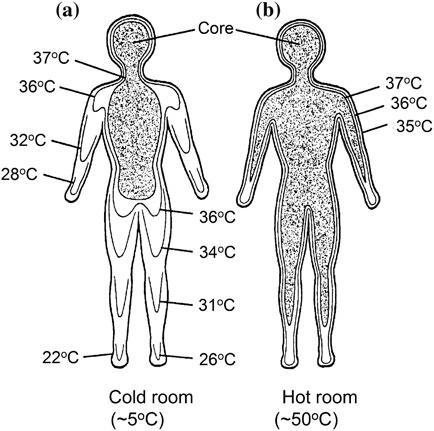
\includegraphics[width=0.5\textwidth]{625.png}
  \caption{Temperatura en el cuerpo en entornos fríos y calientes (de \cite{38}. Cortesía de Robert A. Freitas Jr., Nanomedicine, Vol. 1 (1999), http://www.nanomedicine.com).}
  \label{fig:625}
\end{SCfigure}



La temperatura en todo el cuerpo varía con la temperatura del entorno. Como se muestra en la Fig. 6.25, estas variaciones pueden ser muy grandes en una habitación fría. Estas distribuciones internas se pueden modelar utilizando las propiedades térmicas del cuerpo (Tabla 6.36) y los modelos de transporte térmico presentados aquí.

Las variaciones de temperatura dentro del cuerpo pueden ser importantes, al igual que la forma en que se miden estas temperaturas. Bajo condiciones normales, las temperaturas de todas las regiones del corazón y los pulmones son las mismas dentro de $\sim 0{,}1\ ^\circ\text{C}$ \cite{92}. Durante la hipotermia, como la causada por la inmersión de cuerpo completo en agua fría, la temperatura medida en el esófago inferior o en la región esofágica cerca del corazón parece seguir bien la temperatura cardíaca. Las temperaturas medidas en el recto cambian mucho más lentamente durante la hipotermia que en estas regiones y pueden proporcionar temperaturas que son falsamente $\sim 1\ ^\circ\text{C}$ superiores a las cercanas al corazón. Esto puede ser significativo debido a que la fibrilación ventricular (véase el Cap. 8) ocurre cuando la temperatura corporal central cae por debajo de $\sim 27\text{--}28\ ^\circ\text{C}$ \cite{26,92}.

\begin{SCfigure}[0.8][htbp]
  \centering
  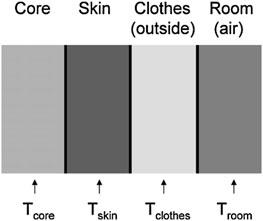
\includegraphics[width=0.55\textwidth]{626.png}
  \caption{Modelo de flujo de calor desde el núcleo del cuerpo hacia el aire.}
  \label{fig:626}
\end{SCfigure}



Relacionemos la temperatura en el interior del cuerpo o núcleo, $T_{\text{core}}$, de la piel, $T_{\text{skin}}$, en el exterior de nuestra ropa, $T_{\text{clothes}}$, y en el aire, $T_{\text{room}}$. Esto se puede visualizar en términos del modelo de la Fig. 6.26, en el cual cada región es una placa rectangular. Modelos más refinados considerarían el cuerpo como un cilindro, como en la Fig. 6.17b \cite{88}.

Siguiendo a (\ref{eq:666}), podemos modelar el flujo entre dos de estas regiones adyacentes mediante
\begin{equation}
(T_1 - T_2) = -I_{12} \frac{1}{A} \left(\frac{dQ}{dt}\right),
\label{eq:672}
\end{equation}
donde el flujo de calor, $dQ/dt$, a través de un área de sección transversal $A$ entre las regiones 1 y 2 está controlado por el aislamiento entre ellas
\begin{equation}
I_{12} = \frac{1}{h_{x, 12}},
\label{eq:673}
\end{equation}
donde $h_{x, 12}$ son los coeficientes de transferencia de calor relevantes entre las dos regiones, tales como los debidos a la radiación, convección, conducción y evaporación.

La diferencia entre la temperatura en el núcleo del cuerpo y en la piel está determinada por el flujo de calor desde el núcleo hacia la piel y el aislamiento del tejido $I_{\text{t}}$, y es
\begin{equation}
T_{\text{core}} - T_{\text{skin}} = -I_{\text{t}} \frac{1}{A} \left[ \left(\frac{dQ}{dt}\right)_r + \left(\frac{dQ}{dt}\right)_c + \left(\frac{dQ}{dt}\right)_v \right],
\label{eq:674}
\end{equation}
donde $(dQ/dt)_r$, $(dQ/dt)_c$ y $(dQ/dt)_v$ son, respectivamente, los flujos de pérdida de calor por radiación, pérdida de calor por convección/conducción y la pérdida de calor por evaporación de humedad en la superficie de la piel. (La pérdida de calor de los pulmones y vías respiratorias no está incluida). Dado que el flujo de calor es desde el núcleo hacia la piel para cada uno, cada término es negativo y la piel está más fría que el núcleo, como es de esperar. El aislamiento proporcionado por el tejido humano tiene un valor máximo de $0{,}10\ ^\circ\text{C-m}^2/\text{W}$ en adultos a temperaturas frías (por debajo de la temperatura crítica) y un valor mínimo de $0{,}03\ ^\circ\text{C-m}^2/\text{W}$ a altas temperaturas. En los bebés, estos valores alto y bajo son de $0{,}05\ ^\circ\text{C-m}^2/\text{W}$ y $0{,}015\ ^\circ\text{C-m}^2/\text{W}$, respectivamente.

La diferencia entre la temperatura en la piel y el exterior de la ropa de una persona es
\begin{equation}
T_{\text{skin}} - T_{\text{clothes}} = -I_{\text{c}} \frac{1}{A} \left[ \left(\frac{dQ}{dt}\right)_r + \left(\frac{dQ}{dt}\right)_c \right],
\label{eq:675}
\end{equation}
donde $I_{\text{c}}$ es el aislamiento de la ropa (o pelaje para los animales). El aislamiento proporcionado por cm de espesor de la ropa humana promedia $0{,}25\ ^\circ\text{C-m}^2/\text{W-cm}$ (Tabla 6.44).

La diferencia entre la temperatura exterior de la ropa de una persona y el aire es
\begin{equation}
T_{\text{clothes}} - T_{\text{room}} = -I_{\text{a}} \frac{1}{A} \left[ \left(\frac{dQ}{dt}\right)_r + \left(\frac{dQ}{dt}\right)_c \right],
\label{eq:676}
\end{equation}
donde $I_{\text{a}}$ es el aislamiento del aire (Tabla 6.42).

\section{Resumen}

La energía utilizada por el cuerpo y la temperatura corporal están determinadas por el metabolismo corporal, que incluye el uso de alimentos, la energía necesaria para hacer funcionar el cuerpo y la producción de calor, y por la pérdida de calor del cuerpo. El valor energético de los alimentos se puede analizar y comparar con la producción de ATP por parte del cuerpo y el uso de ATP en diferentes actividades. La tasa metabólica corporal está compuesta por muchos componentes, cada uno de los cuales se puede modelar. Esto incluye analizar la tasa a la que se necesita energía para el funcionamiento de las funciones corporales de una persona que está inactiva, que se combinan para formar la BMR, y la tasa a la que se necesita energía para que el cuerpo realice actividad física. El metabolismo corporal y la ingesta de alimentos se pueden vincular a modelos del peso corporal en estado estacionario y del aumento y pérdida de peso. El cuerpo puede perder calor por radiación, convección, conducción y evaporación de agua, cada uno de los cuales puede ser modelado y vinculado a modelos que determinan la temperatura corporal.

\section*{Problemas}

\subsection*{Capacidad calorífica}

\begin{enumerate}

\item[6.1] Una persona que pesa $60\text{ kg}$ bebe $600\text{ mL}$ ($0{,}6\text{ kg}$) de agua. Suponga que el agua está a una temperatura que está $25\ ^\circ\text{C}$ por encima o por debajo de la temperatura corporal. ¿Cómo cambia la temperatura corporal? (Utilice el hecho de que el calor específico del agua es $1\text{ kcal/kg-}^\circ\text{C}$, por lo que le suministra al cuerpo una energía de $1\text{ kcal/kg-}^\circ\text{C} \times 0{,}6\text{ kg} \times 25\ ^\circ\text{C}$, y que el calor específico del cuerpo es $0{,}83\text{ kcal/kg-}^\circ\text{C}$). ¿Ayudaría una bebida caliente de este tipo ($+25\ ^\circ\text{C}$) con la hipotermia? ¿Ayudaría una bebida fría de este tipo ($-25\ ^\circ\text{C}$) con la fiebre?

\item[6.2] ¿Cuál es la capacidad calorífica de una célula humana típica de $20\ \mu\text{m}$ de diámetro? Asuma que es una esfera y que tiene un calor específico igual al promedio del cuerpo.

\item[6.3] En una célula humana típica de $20\ \mu\text{m}$ de diámetro, hay aproximadamente $5 \times 10^{-6}\text{ J}$, $2{,}0 \times 10^{-5}\text{ J}$ y $8 \times 10^{-6}\text{ J}$ de energía disponible a partir de carbohidratos, proteínas y grasas, respectivamente. Si toda esta energía se convirtiera en calor, ¿cuál sería el aumento de temperatura en la célula? Utilice los resultados del Problema 6.2 e ignore las pérdidas de calor.

\item[6.4] Una unidad térmica británica (BTU) es la cantidad de calor necesaria para elevar la temperatura de $1\text{ lb}$ de agua en $1\ ^\circ\text{F}$. (Esta unidad, por lo tanto, se define como equivalente al calor específico del agua, que es $1{,}0\text{ cal/g-}^\circ\text{C}$). La cantidad de calor necesaria para congelar agua o derretir hielo (el calor latente de fusión (congelación)) es $80\text{ cal/g} = 335\text{ J/g}$ y la necesaria para vaporizar agua (el calor latente de vaporización) es $543\text{ cal/g} = 2272\text{ J/g}$. (a) Demuestre que $1\text{ BTU} = 1055\text{ J}$. (b) Encuentre el número de BTU requeridos para derretir una libra de hielo. (c) Encuentre el número de BTU requeridos para vaporizar una libra de agua.

\subsection*{Valor calórico}

\item[6.5] Considere la oxidación de la grasa tributirina:
\begin{equation*}
\text{C}_3\text{H}_5\text{O}_3(\text{OC}_4\text{H}_7)_3 + 18{,}5\text{O}_2 \rightarrow 15\text{CO}_2 + 13\text{H}_2\text{O} + 1941\text{ kcal}.
\end{equation*}
(a) Encuentre la energía liberada/g, el equivalente calórico y la relación de intercambio respiratorio (RER) (o cociente respiratorio (RQ)). (b) ¿Son estos valores representativos de una grasa? ¿Por qué sí o por qué no?

\item[6.6] Considere la oxidación del alcohol (etanol): $\text{C}_2\text{H}_5\text{OH} + 3\text{O}_2 \rightarrow 2\text{CO}_2 + 3\text{H}_2\text{O} + 327\text{ kcal}$. (a) Encuentre la energía liberada/g, el equivalente calórico y la relación de intercambio respiratorio (RER) (o cociente respiratorio (RQ)). (b) Compare estos valores con los de los carbohidratos, las proteínas y las grasas.

\item[6.7] Determine el contenido energético en una onza líquida de licor de graduación $86$ (86 proof) a partir del contenido calórico del alcohol. (Una graduación de $200$ (200 proof) significa que la fracción de volumen de alcohol es del $100\%$).

\item[6.8] Demuestre que el volumen de alcohol en un chupito (1~oz) de licor, una copa de vino y una botella de cerveza es aproximadamente el mismo y, por lo tanto, tienen el mismo contenido energético (utilice la Tabla 6.5).

\item[6.9] ¿Son las densidades de energía por unidad de masa para los carbohidratos, las proteínas y las grasas enumeradas en la Tabla 6.3 consistentes con los valores de la Tabla 6.2?

\item[6.10] (a) Deduzca expresiones generales para el porcentaje de energía proveniente de los carbohidratos y las grasas y la energía térmica por L de oxígeno consumido para una RER arbitraria entre $0{,}71$ y $1{,}00$. (b) Determine el porcentaje de kcal proveniente de los carbohidratos y las grasas y la energía térmica por L de oxígeno consumido para cada una de estas RER: $0{,}71$, $0{,}75$, $0{,}80$, $0{,}85$, $0{,}90$, $0{,}95$ y $1{,}00$.

\item[6.11] Muestre cómo el redondeo de las masas de carbohidratos, proteínas y grasas en el donut estándar al valor entero de gramos más cercano puede conducir fácilmente a la diferencia en el contenido calórico calculado y el listado. (Demuestre que esto es cierto incluso ignorando el probable redondeo del contenido calórico total a la decena de kcal más cercana; por lo que $280\text{ kcal}$ podría significar cualquier valor desde $275{,}1$ hasta $284{,}9\text{ kcal}$). Asuma que los carbohidratos y las proteínas tienen un contenido calórico de $4{,}0\text{ kcal/g}$ y las grasas tienen un contenido calórico de $9{,}0\text{ kcal/g}$.

\item[6.12] Repita el Problema 6.11, asumiendo que los contenidos de masa son exactos pero considerando ahora las incertidumbres en los contenidos calóricos de los carbohidratos, proteínas y grasas del donut.

\item[6.13] El Rich Frosted Donut de Entenmann's\textsuperscript{TM}, designado en el texto como nuestro donut estándar, se vendió como un artículo independiente durante muchos años y, hasta 2006, todavía estaba disponible en el paquete de donuts variados con el mismo contenido nutricional. En 2006, el Rich Frosted Donut en empaque individual tenía un contenido nutricional algo diferente: $26\text{ g}$ de grasa, $29\text{ g}$ de carbohidratos, $2\text{ g}$ de proteína y una masa total de $64\text{ g}$. Compare su contenido calórico con el de nuestro donut estándar.

\item[6.14] El Glazed Donut de Entenmann's\textsuperscript{TM} tiene $13\text{ g}$ de grasa, $34\text{ g}$ de carbohidratos, $2\text{ g}$ de proteína y una masa total de $60\text{ g}$ (hasta 2006). (a) Compare su contenido calórico según lo indicado en el paquete ($260\text{ kcal}$) con el de nuestro donut estándar. (b) Encuentre el porcentaje de calorías que provienen de la grasa. (c) Encuentre el porcentaje de la masa del donut que no proviene de grasas, carbohidratos o proteínas.

\item[6.15] El etiquetado del paquete de la versión de 2014 del Rich Frosted Donut de Entenmann's\textsuperscript{TM} (empaque estándar, no un paquete variado) dice que un donut contiene $18\text{ g}$ de grasa, $27\text{ g}$ de carbohidratos y $2\text{ g}$ de proteína, lo cual representa $47\text{ g}$ de la masa total declarada de $55\text{ g}$ del donut. Muestre que, utilizando el mismo método que en el texto, esto sugiere que hay $278\text{ kcal}$ (278 calorías alimentarias) por donut. ¿Cómo se puede reconciliar esto con la afirmación en el paquete de que hay $270\text{ kcal}$ por donut?

\item[6.16] ¿Es la afirmación en el sitio web de Entenmann's\textsuperscript{TM} (descargado el 19 de mayo de 2015) de que la versión de 2015 del Rich Frosted Donut de Entenmann's\textsuperscript{TM} tiene $300\text{ kcal}$ por donut consistente con la información de que este donut de $60\text{ g}$ tiene $20\text{ g}$ de grasa, $30\text{ g}$ de carbohidratos y $2\text{ g}$ de proteína?

\item[6.17] ¿Para cuáles alimentos de la Tabla 6.5 los contenidos calóricos de los carbohidratos, las proteínas y las grasas no explican el valor calórico total? ¿Por qué?

\item[6.18] Sabemos que las grasas tienen aproximadamente $9\text{ kcal/g}$ de contenido energético y las proteínas y carbohidratos tienen alrededor de $4\text{ kcal/g}$. Explique ¿por qué la energía metabolizable por unidad de masa de los alimentos en las Tablas 6.5 y 6.6 es tan diferente de estos números? En particular, ¿por qué los valores para la leche y las zanahorias son tan bajos? ¿Qué podemos aprender sobre la avena y la harina? ¿Qué aprende sobre la mantequilla y los frutos secos?

\item[6.19] Cierta fruta tiene una energía metabolizable de $0{,}4\text{ kcal/g}$ normalmente y de $2{,}4\text{ kcal/g}$ después de haber sido secada. Asuma que la fruta consiste únicamente en agua, azúcar y materia no metabolizable, y encuentre la fracción de cada uno en la fruta y en la fruta después de ser secada.

\item[6.20] Determine el contenido energético por unidad de masa ($\text{kcal/g}$) para cada alimento no alcohólico en la Tabla 6.5. Explique la variación en términos de las cantidades relativas de carbohidratos/proteínas/grasas, agua y «ceniza».

\item[6.21] Determine el porcentaje de calorías provenientes de la grasa para cada alimento no alcohólico en la Tabla 6.5.

\item[6.22] Si la leche descremada es simplemente leche entera menos la grasa, determine el contenido calórico, la masa de carbohidratos, proteínas y grasas, y el $\%$ de agua de 1 taza ($245\text{ g}$) de leche descremada.

\item[6.23] ¿Cuánto aceite hay en las papas fritas? Más precisamente, ¿qué fracciones de la masa y del valor calórico de las papas fritas se deben al aceite y qué fracciones se deben a la papa? Utilice los datos proporcionados en la Tabla 6.5. Ignore la piel de la papa y considere la posibilidad de que se pierda agua en el proceso de fritura. El aceite es pura grasa. ¿Cuánta agua se pierde en el proceso de fritura?

\item[6.24] La yema de un huevo crudo grande tiene una masa de $17\text{ g}$, de los cuales $3\text{ g}$ son de proteína y $5\text{ g}$ son de grasa (y una cantidad traza es de carbohidratos). Tiene un total de $59\text{ kcal}$ de contenido energético y es $49\%$ agua. Determine los valores correspondientes para la clara del huevo, utilizando la Tabla 6.5.

\item[6.25] Para el vino y la cerveza enumerados en la Tabla 6.5, calcule el número de kcal y la masa ($\text{g}$) debido al alcohol (etanol) en cada uno, y la fracción de volumen de alcohol en cada uno, asumiendo que el etanol tiene una densidad de masa de $0{,}79\text{ g/cm}^3$.

\item[6.26] La determinación del calor de combustión de las proteínas a partir de su contenido de nitrógeno debe hacerse con cuidado \cite{68}. (a) Aproximadamente el $60\%$ del nitrógeno en las papas se debe a proteínas y el $40\%$ a la asparagina. Asuma que hay $6{,}25\text{ g}$ de proteína por gramo de N, con un calor de combustión de $5{,}8\text{ kcal/g}$ de proteína, y $4{,}7\text{ g}$ de asparagina por gramo de N, con un calor de combustión de $3{,}45\text{ kcal/g}$ de asparagina. Demuestre que esto significa que hay $28{,}24\text{ kcal}$ en los $5{,}63\text{ g}$ de compuestos nitrogenados provenientes de $1\text{ g}$ de N, lo cual corresponde a un valor promedio de $5{,}02\text{ kcal}$ por gramo de compuesto nitrogenado en las papas. (b) ¿Qué calor de combustión se determinaría para el material nitrogenado con $1\text{ g}$ de N, si utiliza este calor de combustión promedio y la suposición errónea de que hay $6{,}25\text{ g}$ de proteína por gramo de N en este alimento? (c) Repita esto para la suposición errónea de que todo el N medido se debe a proteínas.

\item[6.27] Usted come una libra de comida. Sabe que el $10\%$ de su peso es agua, el $5\%$ de su peso proviene de sólidos no digestibles y el $30\%$ de sus calorías provienen de la grasa. ¿Cuántas calorías ha ingerido?

\item[6.28] En una dieta hipotética propuesta, se supone que una persona deriva el $40 \pm 5\%$, $30 \pm 5\%$ y $30 \pm 5\%$ de sus calorías de carbohidratos, proteínas y grasas, respectivamente. (a) Utilice la Tabla 6.5 para diseñar dos planes de dieta diferentes para una dieta de $2000\text{ kcal/día}$, utilizando alimentos muy diferentes en cada plan. (b) ¿Qué dieta tiene una masa diaria más ligera y, por lo tanto, es quizás mejor para viajes de excursionismo o espaciales? ¿Por qué es así?

\item[6.29] (a) Usted está en una barra de ensaladas y desea ingerir $600\text{ kcal}$. Si asume que la comida es $20\%$ agua (en masa) y $5\%$ cenizas, ¿cuánta comida debe servirse (en oz y g) si asume que del porcentaje restante el $50\%$ son carbohidratos, el $20\%$ es proteína y el $30\%$ es grasa? (b) Para esta cantidad de comida, ¿cuál sería el valor calórico si el contenido sin agua ni cenizas fuera en realidad todo carbohidratos, todo proteínas o todo grasas?

\item[6.30] La energía liberada por tonelada de TNT (trinitrotolueno) detonada es $4{,}18 \times 10^9\text{ J}$. ¿En cuántas toneladas de nuestros donuts estándar se encuentra la misma energía alimentaria?

\item[6.31] Un cuerpo consume $0{,}3\text{ L-atm}$ de oxígeno cada minuto. (a) Determine la tasa de producción de calor si solo se están consumiendo carbohidratos. (b) Determine la tasa de producción de calor si solo se están consumiendo grasas.

\subsection*{Tasas metabólicas}

\item[6.32] La energía libre de Gibbs $\Delta G$ de una reacción química es la energía disponible cuando ocurre a una temperatura constante $T$ y presión constante ($1\text{ atm}$). La energía libre de la hidrólisis del ATP (\ref{eq:616}) es $\Delta G^0 = -7{,}3\text{ kcal/mol}$ bajo las condiciones estándar de $T = 298\text{ K}$, $1\text{ atm}$, $\text{pH} = 7{,}0$ y concentraciones iguales $1\text{ M}$ (molar, mol/L) de todos los reactivos y productos. Para otras condiciones, es $\Delta G = \Delta G^0 + RT \ln(K/K^0)$, donde $R$ es la constante de los gases ($1{,}987\text{ cal/mol-K}$), $T$ es la temperatura para la condición, $K$ es el producto de reacción para la condición y $K^0$ es la constante de equilibrio para condiciones estándar \cite{75}. El producto de reacción es el producto de las concentraciones de los productos (ADP y $\text{P}_i$ aquí) dividido por el de los reactivos (ATP aquí). (Las concentraciones de otros productos y reactivos en (\ref{eq:616}), como el $\text{H}_2\text{O}$, son esencialmente las mismas para las diferentes condiciones y no necesitan ser incluidas. ¿Por qué?). (a) Calcule la energía libre a $T = 310\text{ K}$ en la célula de un eritrocito humano (glóbulo rojo) representativo con concentraciones de $2{,}25\text{ mM}$ (milimolar, milimol/L) para ATP, $0{,}25\text{ mM}$ para ADP y $1{,}65\text{ mM}$ para $\text{P}_i$. (b) En el músculo en reposo, se cree que la concentración de ADP libre está entre $1$ y $37\ \mu\text{M}$ (micromolar). Calcule la energía libre a $T = 310\text{ K}$ si la concentración de ADP es de $25\ \mu\text{M}$ (y las otras concentraciones son las mismas que en (a)). ¿Cómo se comparan estos valores en (a) y (b) con los dados en el texto? (Aparte de la diferencia en los tipos de células, la principal diferencia con la parte (a) es que la concentración relevante es la de ADP libre y no la de ADP total, que incluye el ADP libre y el unido a proteínas celulares). (c) ¿Cómo afecta el uso de tales energías libres bajo condiciones celulares en lugar de aquellas para condiciones estándar al cálculo de la eficiencia de conversión de glucosa en ATP por parte del cuerpo en relación con la de la oxidación de la glucosa?

\item[6.33] Encuentre cuál sería la eficiencia del uso corporal de glucosa si en el metabolismo aeróbico $1\text{ mol}$ de glucosa produjera $36\text{--}38\text{ mol}$ de ATP (el factor de conversión a menudo citado hace varios años), en lugar del rango actualmente aceptado de $30\text{--}32\text{ mol}$, como se indica en el capítulo. Asuma que la energía liberada por el ATP es de $14{,}0\text{ kcal/mol}$.

\item[6.34] Asuma que la oxidación de la glucosa extrae toda la energía libre posible. Encuentre el número máximo de moléculas de ATP que podrían formarse si la hidrólisis del ATP fuera $100\%$ eficiente. Asuma que la energía liberada por el ATP es de $14{,}0\text{ kcal/mol}$.

\item[6.35] Suponga que en el metabolismo aeróbico $1\text{ mol}$ de glucosa puede producir $32\text{ mol}$ de ATP, mientras que bajo condiciones similares $1\text{ mol}$ de carbohidratos del glucógeno puede producir $33\text{ mol}$ de ATP. Dado que el glucógeno es fabricado por el cuerpo a partir de la glucosa, ¿está obteniendo el cuerpo $1\text{ mol}$ adicional de ATP de forma gratuita al convertir primero la glucosa en glucógeno y luego usarla, o realmente está sucediendo algo más? Explique.

\item[6.36] La energía libre estándar para la hidrólisis de ADP a AMP (monofosfato de adenosina) es de $-7{,}8\text{ kcal/mol}$. ¿Cuál es para condiciones celulares? Asuma las condiciones para un eritrocito en el Problema 6.32a y una concentración de AMP de $0{,}2\text{ mM}$ \cite{75}.

\item[6.37] Repita el Problema 6.32 para el ácido palmítico.

\item[6.38] (a) La masa molar del ATP es de $507\text{ g}$. Si una persona de $60\text{ kg}$ tiene una tasa metabólica de $2000\text{ kcal/día}$ y el ATP libera $14{,}0\text{ kcal/mol}$ durante la hidrólisis, ¿qué masa de ATP necesitaría esa persona al día si el ADP formado después de la hidrólisis del ATP no se reciclara de nuevo a ATP? (b) ¿Cómo se compara esto con la masa de la persona? (c) ¿Cuántos ciclos de hidrólisis y recreación de ATP realiza una molécula de ATP promedio por día y por minuto si hay un total de $0{,}2\text{ mol}$ de ATP en el cuerpo? (d) Repita cada parte para un ATP que libera $7{,}3\text{ kcal/mol}$ durante la hidrólisis.

\item[6.39] (a) La masa molar del ATP es de $507\text{ g}$. ¿Cuántas kcal estarían disponibles para el cuerpo si toda la masa en reposo de una molécula de ATP se convirtiera en energía (útil)? Utilice $E = mc^2$. (b) ¿Qué masa de ATP (en g) utilizaría una persona con una tasa metabólica de $2000\text{ kcal/día}$ si todo el ATP se convirtiera en energía? (c) Si una planta de energía nuclear de $1\text{ GW}$ convirtiera esta energía de ATP en energía eléctrica con una eficiencia del $20\%$, ¿cuánto ATP utilizaría (en g) por segundo y por año? (d) En las reacciones nucleares, solo una fracción de la masa en reposo se convierte en energía. Repita (a)--(c) si esa fracción fuera $2{,}5 \times 10^{-5}$, que es la fracción de energía de masa en reposo convertida en energía cinética en la desintegración de partículas alfa $^{241}\text{Am} \rightarrow \alpha + ^{237}\text{Np}$.

\item[6.40] Esboce en el mismo conjunto de ejes etiquetados la tasa disponible de uso de ATP (normalizada a su valor máximo posible) frente al tiempo para una persona que comienza actividades físicas moderadas en $t = 0$, para cada uno de los siguientes casos: (a) Solo el sistema de fosfágenos está disponible. (b) No hay mucho oxígeno disponible, por lo que solo los sistemas de fosfágenos y glucólisis anaeróbica están disponibles. (c) Hay mucho oxígeno disponible, por lo que se utilizan los sistemas de fosfágenos y metabolismo aeróbico.

\item[6.41] La potencia máxima anaeróbica máxima para los hombres es de $2{,}1\text{ hp}$ y la tasa metabólica máxima durante la glucólisis anaeróbica es de $1{,}6\text{ mol de ATP/min}$. ¿Son estas tasas consistentes? ¿Por qué? (Asuma aquí $10\text{ kcal}$ por mol de ATP).

\item[6.42] La Tabla 6.3 muestra que el ATP almacena mucha menos energía por unidad de volumen y masa que otros combustibles. ¿Por qué entonces es tan importante?

\item[6.43] El ácido esteárico es un ácido graso de cadena de 18 carbonos que se somete a 8 ciclos completos en el metabolismo aeróbico. ¿Cuántos moles de ATP se forman por mol de ácido esteárico?

\item[6.44] Utilice los datos de la Tabla 6.22 para encontrar cuál sería la potencia máxima de salida de un ser humano (en W) si todo el volumen humano estuviera compuesto por células tisulares típicas que funcionan a la potencia máxima de salida. ¿Supera esto la potencia máxima de salida del cuerpo humano indicada? ¿Es esto razonable? ¿Por qué?

\item[6.45] (a) Si el volumen habitual de una persona estuviera ocupado únicamente por motores musculares de miosina empaquetados estrechamente, ¿cuál sería la potencia consumida por el cuerpo (en W) y cómo se compara esto con las tasas metabólicas basal y máxima? (b) ¿Cuál sería la tasa de aumento de temperatura del cuerpo para tal volumen, asumiendo que la capacidad calorífica es la de un ser humano normal y no hay pérdidas de calor?

\item[6.46] ¿Cuántos puentes cruzados de miosina se necesitarían para propulsar un auto de $200\text{ hp}$? (Asuma los datos para las moléculas de miosina en la Tabla 6.22). ¿Cómo se compara esto con el número de puentes cruzados en un ser humano típico?

\subsection*{Tasas metabólicas basales}

\item[6.47] Utilice la regla de Kleiber para comparar la BMR por unidad de masa (con unidades generales de $\text{kcal/kg-día}$) para un ratón ($30\text{ g}$), un ser humano ($70\text{ kg}$) y una ballena azul ($10^5\text{ kg}$).

\item[6.48] ¿Compare la tasa metabólica esperada para el hombre estándar del Cap. 1 utilizando la regla de Kleiber y las ecuaciones de Harris--Benedict? ¿Por qué son diferentes? ¿Es esto razonable o no?

\item[6.49] ¿Cuántos donuts estándar debe comer diariamente una persona de $60\text{ kg}$ para mantener su BMR, asumiendo la regla de Kleiber?

\item[6.50] ¿Cuánta comida tendría que comer cada día (en g) para equilibrar una tasa metabólica basal (BMR) de $1700\text{ kcal/día}$ si solo comiera (a) glucosa o (b) grasa (típica)?

\item[6.51] Otra formulación de las ecuaciones de Harris--Benedict (\ref{eq:628}) y (\ref{eq:629}) utiliza números redondeados:
\begin{equation}
\text{Para hombres: BMR} = 66 + 13{,}7 m_{\text{b}} + 5 H - 6{,}9 Y
\label{eq:677}
\end{equation}
\begin{equation}
\text{Para mujeres: BMR} = 665 + 9{,}6 m_{\text{b}} + 1{,}7 H - 4{,}7 Y,
\label{eq:678}
\end{equation}
donde el BMR está en $\text{kcal/día}$, $m_{\text{b}}$ es la masa corporal en kg, $H$ es la altura en cm y $Y$ es la edad en años. ¿Qué tan diferentes son las dos formulaciones para un hombre de $6\text{ ft}$ de estatura, $25\text{ años}$ de edad y un peso de $200\text{ lb}$, y una mujer de $5\text{ ft } 2\text{ in.}$, $50\text{ años}$ de edad y un peso de $125\text{ lb}$? ¿Son significativas estas diferencias?

\item[6.52] ¿Qué tanto más alta es la BMR para una mujer embarazada? Estime esto considerando el aumento en su BMR a partir de dos factores. Ella debe suministrar alimentos para formar el feto junto con la estructura de soporte en el útero y debe suministrar la energía para el BMR del feto. (Ella está literalmente «comiendo por dos»). Asuma que se encuentra al final del embarazo y que está ganando $4\text{ lb}$ al mes de tejido humano típico, asumiendo que esto no incluye la retención de líquido adicional fuera del útero. Asuma que el feto tiene la BMR de un bebé al nacer que pesa $7\text{ lb}$ (y use las tablas de BMR para niños menores de $3\text{ años}$).

\item[6.53] Se estima que una ganancia de peso gestacional de $12\text{ kg}$ durante el embarazo incluye $597\text{ g}$ de proteína y $3{,}74\text{ kg}$ de grasa. ¿Cuánta energía calórica requiere esto? (Utilice $5{,}65\text{ kcal/g}$ de proteína y $9{,}25\text{ kcal/g}$ de grasa \cite{18}). ¿Qué fracción de la ingesta calórica adicional total de $77\,000\text{ kcal}$ durante el embarazo representa esto?

\item[6.54] Durante el transcurso del embarazo, la BMR de una mujer inicialmente de $67\text{ kg}$ aumenta de $1300$ a $1720\text{ kcal/día}$, a medida que gana $18{,}5\text{ kg}$ \cite{58}. ¿Se puede entender esto utilizando el escalamiento de $m_{\text{b}}^{3/4}$ o las relaciones de la Tabla 6.19?

\item[6.55] (a) ¿Cuántos donuts estándar necesitaría comer una futura madre para suministrar las necesidades de energía adicionales totales de $\sim 90\,000\text{ kcal}$ durante el transcurso del embarazo? (b) ¿Cuántos donuts necesitaría comer por cada uno de los $280\text{ días}$ de gestación? (c) ¿Cómo cambiaría esta respuesta sabiendo que la ingesta calórica adicional es necesaria únicamente en la segunda mitad del embarazo?

\item[6.56] Usted le dice a un hombre de $80\text{ kg}$ que ha estado sentado e inactivo durante algún tiempo que no es diferente de una bombilla incandescente de $80\text{ W}$. ¿Qué tan precisa es su afirmación en términos de: (a) la potencia total emitida, (b) la potencia emitida por unidad de volumen, (c) el costo aproximado de la energía producida (en términos de centavos de dólar por $\text{kW-h}$), (d) los tipos de energía que se producen, (e) los tipos de energía que ingresan, (f) el espectro de cualquier luz (radiación electromagnética) que se emita y (g) el flujo de gases hacia y desde cada objeto?

\item[6.57] Si fuera a hacer esencialmente la misma afirmación que en el Problema 6.56 con respecto a una bombilla de diodo emisor de luz (LED), ¿cuál sería la potencia en vatios de esa bombilla (para las luces LED más actuales)?

\item[6.58] Utilice la Fig. 6.14 para encontrar la potencia metabólica (en $\text{kcal/día}$) que tiene una persona en inanición al metabolizar las reservas de energía almacenadas en el cuerpo durante la cuarta semana de inanición. ¿Cómo se compara esto con una tasa metabólica basal típica?

\item[6.59] ¿Tiene sentido cuantitativo la tasa metabólica basal por unidad de volumen para un ser humano, dadas las tasas metabólicas basales para diferentes células y la fracción del cuerpo que contiene células (Tabla 6.22)?

\subsection*{Tasas metabólicas durante actividades}

\item[6.60] En un salto de altura, una persona de $70\text{ kg}$ eleva su centro de masa en $51\text{ cm}$ durante una fase de extensión (con aceleración constante) que toma $0{,}25\text{ s}$. (a) ¿Cuál es la energía cinética de la persona al despegar? (b) Si la eficiencia muscular es del $20\%$, ¿cuánta energía química se utiliza para realizar un salto? (Exprese su respuesta en julios y en kcal (las calorías alimentarias habituales)). (c) ¿Cuál es la potencia promedio generada por la persona durante el salto en vatios y caballos de fuerza ($1\text{ caballo de fuerza (hp)} = 746\text{ W}$)? (d) ¿Con qué frecuencia tendría que saltar alguien (durante un ciclo de vigilia de $12\text{ h}$) para aumentar su tasa de metabolismo (promedio diario) al doble del valor basal (que es $1500\text{ kcal/día}$)?

\item[6.61] Utilice la Fig. 3.26 para encontrar las tasas metabólicas (en $\text{kcal/h}$) para correr a velocidades de $2$ y $4\text{ m/s}$, para personas de $50$ y $90\text{ kg}$ en cada caso. ¿Ha incluido la BMR?

\item[6.62] Convierta los datos sobre capacidades aeróbicas en el párrafo que describe las capacidades de las personas de $\text{mL/kg-min}$ a $\text{kcal/h}$ para hombres de $70\text{ kg}$ y mujeres de $50\text{ kg}$.

\item[6.63] La tasa metabólica al caminar, MR en $\text{cal/min}$, se ha determinado midiendo la tasa de consumo de oxígeno, en función de la velocidad de marcha, $v$ en $\text{m/min}$:
\begin{equation}
\text{MR} = 0{,}267 v^2 + 2160.
\label{eq:679}
\end{equation}
(a) Determine la velocidad de marcha en la cual la energía gastada por unidad de distancia es mínima, en $\text{m/min}$, $\text{m/s}$ y $\text{mph}$ (millas por hora) \cite{50}. ¿Cómo se compara esto con el mínimo mostrado en la Fig. 3.26? (b) Determine la tasa de consumo de energía a esta velocidad óptima en $\text{kcal/h}$.

\item[6.64] Determine cuánta energía utiliza una persona de $70\text{ kg}$ para correr un maratón en terreno plano.

\item[6.65] (a) Demuestre que la tasa de cambio de la energía potencial al caminar o correr a una velocidad $v$ en una pendiente con un ángulo $\theta$ (positivo para cuesta arriba, negativo para cuesta abajo) es $m_{\text{b}}gv \sin \theta$. (b) Considere las necesidades metabólicas para una caminata lenta de una mujer de $50\text{ kg}$, asumiendo que el costo de energía de caminar por encima del de estar de pie es de $2{,}13\text{ J/kg-m}$ a $1{,}2\text{ m/s}$ ($2{,}6\text{ mph}$). Asuma que el trabajo y la potencia requeridos para ir cuesta arriba es aproximadamente $2{,}7 \times$ el aumento en la energía potencial, y al moverse cuesta abajo se necesita menos potencia que en terreno plano en aproximadamente el $50\%$ de la tasa de disminución de la energía potencial. Encuentre la necesidad metabólica promedio (total) en $\text{kcal/min}$ para esta persona que camina a esta velocidad constante: (i) en una superficie plana, (ii) en una pendiente cuesta arriba del $10\%$, (iii) en una pendiente cuesta abajo del $10\%$ y (iv) cuando la mitad es en pendiente cuesta arriba del $10\%$ y la otra mitad en pendiente cuesta abajo del $10\%$ (de modo que la elevación final es la misma que la inicial). (v) ¿Cómo se compara la respuesta en (iv) con la de (i)? (c) Si quisiera mantener su tasa metabólica ya sea que caminara sobre una superficie plana, cuesta arriba o cuesta abajo en la parte (b), ¿qué tan rápido caminaría cuesta arriba y cuesta abajo, asumiendo que en terreno plano se movía a la velocidad $v$ de la parte (b)?

\item[6.66] Considere al velocista en aceleración del Cap. 3. ¿Cuál es la tasa metabólica del velocista (en $\text{kcal/min}$) si la eficiencia de conversión de energía metabólica en energía mecánica es del $20\%$? ¿Cuánta energía metabólica consume el velocista en una carrera de $100\text{ m}$?

\item[6.67] (a) Determine la tasa metabólica y las tasas de consumo de oxígeno para cada etapa del Protocolo de Bruce para un varón de $75\text{ kg}$. (b) ¿Cuántas kcal se queman en cada etapa y cuál es la energía total quemada si el paciente finaliza todas las etapas?

\item[6.68] (a) Determine la tasa metabólica y las tasas de consumo de oxígeno para cada etapa del Protocolo de Naughton para un varón de $75\text{ kg}$. (b) ¿Cuántas kcal se queman en cada etapa y cuál es la energía total quemada si el paciente finaliza todas las etapas?

\item[6.69] ¿Cómo se comparan las tasas metabólicas en las etapas más altas del Protocolo de Bruce y de Naughton?

\item[6.70] En la calorimetría indirecta, las tasas de consumo de $\text{O}_2$, $dV_{\text{O}_2}/dt$, y de producción de $\text{CO}_2$, $dV_{\text{CO}_2}/dt$, se determinan mientras el sujeto realiza una actividad física. (a) Describa cómo se pueden determinar midiendo las tasas de volumen de aire inspirado y espirado, $dV_{\text{air}}/dt$, y las fracciones de $\text{O}_2$ y $\text{CO}_2$ tanto en el aire inspirado como en el espirado. (b) Un sujeto inspira y espira aire a una tasa de $100\text{ L/min}$, el aire inspirado es $21\%\ \text{O}_2$ y el aire espirado es $16\%\ \text{O}_2$. Demuestre que $dV_{\text{O}_2}/dt$ es de $5\text{ L/min}$. (c) ¿Cuál es la tasa metabólica del sujeto en $\text{kcal/min}$? (d) ¿En qué tipo de actividad podría estar participando el sujeto?

\item[6.71] A partir de la discusión después de (\ref{eq:618}), ¿qué es $p_a - p_v$ en la sangre en el sistema (en mL de $\text{O}_2$/L de sangre)?

\item[6.72] (a) Si la energía necesaria para cubrir las necesidades de metabolismo basal de un varón de $70\text{ kg}$ durante un día se utilizara para aumentar la energía potencial gravitatoria de esa persona con un $100\%$ de eficiencia, ¿qué tan alto sería elevada esa persona? (b) Si una persona puede subir escaleras con una eficiencia mecánica del $20\%$, ¿qué tan alto puede subir utilizando la energía metabólica diaria descrita en la parte (a)? ¿A cuántos pisos aproximadamente corresponde esto?

\item[6.73] En el fútbol americano, un liniero ofensivo y uno defensivo, cada uno de $300\text{ lb}$, se enfrentan, agachados en una «posición» de salida, separados por $2\text{ yardas}$ (lo cual es una ligera sobreestimación). Cuando comienza una «jugada», corren el uno hacia el otro, acelerando cada uno a $g/2$, chocan y pasan los siguientes $5\text{--}10\text{ s}$ empujándose mutuamente sin movimiento en este modelo. Considere a uno de los linieros, por ejemplo, el liniero ofensivo. (a) ¿Cuánta energía cinética desarrolla antes de la colisión (en J)? (b) Si convierte energía metabólica en esta energía cinética con una eficiencia del $10\%$ y juega $50\text{ jugadas}$ por partido, ¿cuánta energía metabólica utiliza en un partido (en kcal)? (c) Se dice que los linieros utilizan hasta $10\,000\text{ kcal}$ en un partido. ¿Respalda su respuesta en (b) esta afirmación? Si no es así, ¿por qué?

\item[6.74] Como se describe en el Cap. 7, una persona intenta volar agitando sus brazos. Suponga que al comienzo de cada aleteo cada brazo comienza sin energía cinética y al final del aleteo cada brazo se mueve a una velocidad promedio de $20\text{ m/s}$. (a) Si esta energía cinética de los brazos necesita generarse $3\text{ veces}$ por segundo, y el cuerpo convierte la energía metabólica en esta energía mecánica con una eficiencia del $10\%$, ¿cuántas $\text{kcal/min}$ consumiría un cuerpo de $70\text{ kg}$ en este intento de volar? (Utilice los datos antropométricos del Cap. 1 para determinar la masa de los brazos). (b) ¿Sería difícil para una persona continuar con este intento infructuoso y bastante absurdo de volar durante mucho tiempo? ¿Por qué?

\item[6.75] Una persona levanta una masa de $15\text{ kg}$ desde el suelo hasta por encima de su cabeza (una distancia de $2\text{ m}$). ¿Cuántas veces tiene que hacer esto para perder una libra de grasa, asumiendo una eficiencia muscular del $25\%$?

\item[6.76] Una mujer de $50\text{ kg}$ realiza $10\text{ dominadas}$ (chin-ups) en un minuto (cada una elevando su centro de masa en $0{,}5\text{ m}$). Después de $5\text{ min}$, ¿cuánto trabajo mecánico ha realizado (en J) y cuánta energía metabólica ha utilizado (en kcal), asumiendo una eficiencia muscular del $25\%$?

\item[6.77] ¿Cuánta energía (energía potencial gravitatoria) se requiere para elevar a una persona de $70\text{ kg}$ en $1\text{ m}$ (en kcal)? Si sus músculos pueden hacer esto con una eficiencia del $25\%$, ¿cuántas veces tendría que levantar a esa persona para quemar el contenido calórico de un donut estándar ($280\text{ kcal/donut}$)?

\item[6.78] Después de una carrera larga, usted camina durante $10\text{ min}$ a un ritmo pausado. ¿Es su tasa metabólica la misma que para caminar en la Tabla 6.21? ¿Por qué?

\item[6.79] Usted corre durante media hora y gasta $300\text{ kcal/h}$ por encima de la BMR durante ese tiempo. Después de correr, jadea y resopla durante otros $5\text{ min}$. Estime el número de kcal que gasta en exceso de la cantidad de la BMR durante este tiempo. ¿Es esto significativo?

\item[6.80] Determine la energía metabólica mínima en kcal que una persona de $50\text{ kg}$ necesita gastar para impulsar un columpio de $3\text{ m}$ de longitud hasta que el columpio forme un ángulo de $60\ ^\circ$ con la vertical, si la eficiencia muscular es del $20\%$.

\item[6.81] Las tasas metabólicas máximas a corto plazo son mucho mayores que las tasas promedio que podemos mantener durante largos períodos. Estimémoslas asumiendo que operamos a esta tasa máxima cuando lanzamos una pelota de masa $m = 1\text{ kg}$ a una distancia $d = 60\text{ m}$. Esto se hace lanzándola a una velocidad $v$ con un ángulo de salida de $45\ ^\circ$ e ignorando la resistencia del aire. Ignore también la diferencia entre el punto de despegue y el de caída en la trayectoria de la pelota. (a) Demuestre que la potencia mecánica máxima es $P_{\text{mech}} = mv^2/t + mgv/\sqrt{2}$, donde $t$ es el tiempo necesario para lanzar el objeto acelerando los brazos (a una tasa constante) sobre una distancia $s$. Tomaremos $s = 1\text{ m}$. (b) Si la eficiencia para realizar trabajo mecánico es $\epsilon$, demuestre que la potencia metabólica máxima necesaria es $P_{\text{met}} = m(gd)^{3/2}/2\epsilon s + mg^{3/2}d^{1/2}/\sqrt{2}\epsilon$. (c) Utilizando los valores dados, demuestre que la tasa metabólica máxima es de aproximadamente $14\,000\text{ W}$ y, por lo tanto, aproximadamente $200\times$ la BMR. (La BMR es aproximadamente la misma —y suele ser mayor— que la tasa máxima a largo plazo para realizar trabajo mecánico. Serían iguales si el factor de actividad promedio diario fuera 2).

\item[6.82] ¿Cómo afectaría la actividad física habitual durante el embarazo a la MR, dado lo que sabe sobre la BMR?

\subsection*{Factores de actividad}

\item[6.83] Estime la tasa metabólica diaria promedio y el factor de actividad de una «ama de casa» de $50\text{ kg}$. (Asuma que $f = \text{MET}$).

\item[6.84] Calcule su factor de actividad $f$ para un día típico. (Asuma que $f = \text{MET}$).

\item[6.85] Una estudiante pasa $6\text{ h}$ al día durmiendo, $11\text{ h}$ sentada (asistiendo a clases (y despierta), comiendo, jugando videojuegos, etc.), $0{,}5\text{ h}$ aseándose y vistiéndose, $4{,}75\text{ h}$ caminando, $1\text{ h}$ de pie, $0{,}25\text{ h}$ jugando baloncesto y $0{,}5\text{ h}$ montando en bicicleta. ¿Cuáles son la MR y el nivel de actividad de la estudiante? (Asuma la BMR de una estudiante de $55\text{ kg}$ y $20\text{ años}$ de edad, y que $f = \text{MET}$).

\subsection*{Pérdida y ganancia de peso}

\item[6.86] Determine cuántos donuts estándar debería comer una persona ($70\text{ kg}$) después de jugar al baloncesto durante $2\text{ h}$ para mantener la misma reserva de energía que la persona (a) tenía antes de jugar al baloncesto o (b) habría tenido después de pasar $2\text{ h}$ sentada en su lugar.

\item[6.87] Una persona de $150\text{ lb}$ ($68\text{ kg}$) consume $2500\text{ kcal}$ todos los días y mantiene un peso estable. Ahora, esta persona decide comer una rebanada de pan extra todos los días ($100\text{ kcal}$) y eventualmente alcanza un nuevo peso de estado estacionario. (a) ¿Cuánto peso gana esa persona (en estado estacionario) si su tasa metabólica total escala, respectivamente, como (i) $m_{\text{b}}^{3/4}$ o (ii) $m_{\text{b}}$ ($m_{\text{b}} = \text{masa corporal}$)? (b) Para ambas relaciones de escalamiento, ¿cuánto peso perderá esa persona si comiera una rebanada de pan menos cada día? (c) Si la persona quiere comer esa rebanada de pan extra todos los días, pero no quiere ganar el peso extra, ¿cuánto tiempo tendría que correr cada día para evitar ganar ese peso extra?

\item[6.88] ¿Cuánto peso ganan las personas con la edad? Considere a un hombre de $30\text{ años}$, $6\text{ ft}$ ($1{,}83\text{ m}$), $150\text{ lb}$ ($68\text{ kg}$) de peso, con un factor de actividad $f = 1{,}5$, y asuma que la BMR de la persona escala como en (\ref{eq:630}) —la cual tiene una fuerte dependencia de $m_{\text{b}}^{3/4}$— y que la tasa metabólica total MR es igual a esta BMR multiplicada por el factor de actividad. Encuentre cuánto peso ganará la persona (hasta su nuevo peso en estado estacionario): (a) cuando cumpla $50\text{ años}$ (con la misma ingesta de alimentos, nivel de actividad, etc.). (b) si el nivel de actividad de este hombre de $30\text{ años}$ disminuye de $1{,}5$ a $1{,}4$ (con la misma ingesta de alimentos, etc.). (c) si la persona de $30\text{ años}$ ($f = 1{,}5$) aumenta su ingesta de alimentos en $100\text{ kcal/día}$ (una rebanada grande de pan al día). (d) si ocurre cada una de las situaciones (a)–(c) (es decir, el hombre de $30\text{ años}$ envejece (ahora tiene $50$), es menos activo (ahora $f = 1{,}4$) y come más ($100\text{ kcal/día}$ más)). (e) ¿Se suman los cambios individuales en (a)–(c) para dar el de (d)? (f) Si la persona en (c) quiere comer esa rebanada de pan extra todos los días, pero no quiere ganar el peso extra, ¿cuánto tiempo tendría que correr cada día para evitar ganar ese peso extra? Puede asumir que la estatura específica permanece constante en su valor inicial en las partes (a)–(d).

\item[6.89] Si su tasa metabólica diaria excede su ingesta calórica en $1000\text{ kcal}$ (lo cual es una diferencia muy grande) durante una semana, ¿cuánto peso perderá? Asuma que el cambio se debe únicamente al uso de grasa corporal para compensar esta diferencia, con $9\text{ kcal}$ por gramo de grasa corporal, de modo que no haya otra pérdida de peso concomitante. (¿Existen otras pérdidas de peso concomitantes? Algunos suplementos para perder peso también pueden provocar una pérdida más trivial de agua corporal).

\item[6.90] En un estudio \cite{15}, hombres sanos y sensibles a la insulina de $\sim 50\text{ años}$ de edad fueron alimentados con una dieta con un contenido energético de $6200\text{ kcal/día}$ durante siete días. Su gasto energético habitual es de $2030\text{ kcal/día}$. Ganaron $3{,}5\text{ kg}$ de masa, toda ella en grasa. ¿Tiene sentido esto? ¿Por qué?

\item[6.91] Si $5\text{ lb}$ ($2{,}3\text{ kg}$) de grasa corporal se convirtieran en $5\text{ lb}$ de músculo corporal, ¿cómo disminuiría eso el nivel de otra grasa corporal debido al aumento de la MR?

\item[6.92] ¿Cuál es la masa en kg y el peso en libras de un hemisferio de tejido humano con un diámetro de $0{,}4\text{ m}$ (siendo la densidad promedio de dicho tejido $0{,}9\text{ g/cm}^3$)? (Este es un modelo del aumento de peso de una mujer embarazada —aparte del debido a la retención de agua— o el debido a una «barriga cervecera» relativamente pequeña).

\item[6.93] Un cambio en la masa corporal de $1\text{ kg}$ es causado por un cambio en la energía metabolizable de aproximadamente $3500\text{ kcal}$. Esto significa que se pueden obtener aproximadamente $3500\text{ kcal}$ de energía química al oxidar $1\text{ kg}$ de materiales de almacenamiento corporal promedio. La relatividad especial enseña que el contenido de energía total de una masa $m$ es $E = mc^2$. ¿Cuánto es esto para $1\text{ kg}$ (en unidades de kcal)? ¿Cuántas veces es esto más grande que la energía química?

\item[6.94] \label{prob:694} El nivel de iones de sodio en el cuerpo depende de la ingesta de sal y de cómo el cuerpo controla dicho nivel. El cuerpo mantiene una concentración de $\text{Na}^+$ de aproximadamente $10\text{ mM}$ (milimolar) para el líquido intracelular (normalmente $\sim 5\text{ L}$) y de aproximadamente $145\text{ mM}$ para el líquido extracelular (normalmente $\sim 2{,}5\text{ L}$, que es la mitad correspondiente al plasma sanguíneo de los $5\text{ L}$ de sangre entera). Supongamos que usted come una bolsa de papas fritas que contiene $2\text{ g}$ de sodio (en forma de iones de sodio) y asumamos que —por el momento— todo permanece en el cuerpo y, en particular, en estos líquidos. Ahora supongamos que el cuerpo responde intentando mantener las concentraciones anteriores de $\text{Na}^+$, por lo que luego usted bebe (y retiene) suficiente agua para mantener estas concentraciones. ¿Cuánto peso ganará, asumiendo que todo el nuevo $\text{Na}^+$ (y, por lo tanto, el agua añadida) va a (a) el agua intracelular, (b) el agua extracelular o (c) ambas, de manera que se mantenga la misma relación de volúmenes de líquidos intracelular y extracelular? (La ingesta diaria recomendada de Na es de aproximadamente $2{,}5\text{ g}$).

\item[6.95] Repita el Problema~\ref{prob:694} para el caso de comer una bolsa grande de pretzels que contiene $8\text{ g}$ de sodio.

\subsection*{Pérdida de calor}

\item[6.96] \label{prob:696} En (\ref{eq:644}) hubo un déficit neto de radiación de $116\text{ W}$ para una temperatura de la pared (y del aire) de $24\ ^\circ\text{C}$. Encuentre el déficit para una temperatura de la pared de $0\ ^\circ\text{C}$.

\item[6.97] Una persona estándar se encuentra en el espacio interestelar. Emite radiación térmica basada en la temperatura de la superficie de su cuerpo y recibe radiación térmica del fondo de cuerpo negro a $3\text{ K}$. ¿Cuánto tiempo tardaría la temperatura de la persona en disminuir en $5\text{ K}$? Asuma que no existen otras fuentes de generación y pérdida de calor, e ignore el hecho de que la persona no viviría mucho tiempo por muchas otras razones. Asuma también que el transporte térmico en el cuerpo ocurre en una escala de tiempo mucho más corta que la que calcula aquí.

\item[6.98] Considere a una persona sentada desnuda en una playa en Florida \cite{19}. En un día soleado, la energía de radiación visible del sol es absorbida por la persona a una tasa de $30\text{ kcal/h}$ o $34{,}9\text{ W}$. La temperatura del aire es de unos cálidos $30\ ^\circ\text{C}$ y la temperatura de la piel del individuo es de $32\ ^\circ\text{C}$. La superficie corporal efectiva expuesta al sol es de $0{,}9\text{ m}^2$. (Asuma esta misma área para la absorción solar, la transferencia de radiación y la pérdida por convección. ¿Es esta una buena suposición?). (a) Encuentre la ganancia o pérdida neta de energía por radiación térmica cada hora. (Asuma la ganancia y pérdida de radiación térmica de acuerdo con (\ref{eq:651}) y una emisividad de $1$). (b) Si hay una brisa de $4\text{ m/s}$, encuentre la energía perdida por convección cada hora (use (\ref{eq:661}), con (\ref{eq:663})). (c) Si la tasa metabólica del individuo es de $80\text{ kcal/h}$ ($93{,}0\text{ W}$) y la respiración representa una pérdida de $10\text{ kcal/h}$ ($11{,}6\text{ W}$), ¿cuánto calor adicional debe perderse por evaporación para mantener constante la temperatura central del cuerpo?

\item[6.99] ¿Qué tan diferentes son (\ref{eq:662}) y (\ref{eq:663}) en el rango donde esta última es válida?

\item[6.100] Una ciclista de carreras produce calor a una tasa de $1300\text{ kcal/h}$ en exceso de la tasa normal. Si todo este exceso de calor se pierde por sudoración y enfriamiento evaporativo, ¿cuántos litros de agua debe beber la ciclista cada hora para mantener sus fluidos corporales (al nivel que habría tenido sin pedalear)?

\item[6.101] ¿Qué sucede cuando la temperatura ambiente supera la temperatura corporal, tanto para la vía de «enfriamiento» por cuerpo negro como por respiración?

\item[6.102] Compare las conductividades térmicas de los materiales de la Tabla~\ref{tab:637} con las de las partes del cuerpo.

\item[6.103] Utilice la Tabla~\ref{tab:637} para explicar por qué es malo confeccionar ropa para clima frío con papel de aluminio, muy bueno hacerla con tejido de algodón y excelente hacerla con capas de tela separadas por aire.

\item[6.104] (a) ¿Qué tan gruesa debe ser su ropa en un día frío? Modele a una persona como un cilindro de $1{,}65\text{ m}$ de altura y $0{,}234\text{ m}$ de diámetro. Asuma que la pérdida de calor es de $1500\text{ kcal/día}$ y ocurre en la circunferencia del cilindro (pero no en la parte superior ni en la inferior). La temperatura de su piel es de $34\ ^\circ\text{C}$ y la temperatura exterior es de $0\ ^\circ\text{C}$. Asuma los valores de aislamiento de la Tabla~\ref{tab:644} y que esta es la única forma significativa de aislamiento. Use la ecuación habitual de flujo de calor para superficies planas y regiones planas (\ref{eq:672}). (b) El flujo de calor radial en un cilindro de radio $r$ se puede modelar asumiendo superficies planas si el espesor $\Delta x$ se reemplaza por $r \ln(1 + \Delta r/r)$. ¿Cómo cambia esto el resultado en (a)?

\item[6.105] El valor R a menudo se utiliza para caracterizar el aislamiento (o resistencia térmica) necesario y utilizado para aislar casas. Es formalmente idéntico al término aislamiento definido en este capítulo. Cuando se expresa en unidades del SI, el valor del aislamiento se denomina valor RSI, de modo que si el aislamiento es de $3\text{ m}^2\text{-}^\circ\text{C/W}$, el valor del aislamiento es RSI-3. (a) En los EE.\,UU., se utiliza el valor de aislamiento en unidades de $\text{ft}^2\text{-}^\circ\text{F-h/BTU}$ y se denomina valor R. Demuestre que un valor R de 10 corresponde a un valor RSI de $1{,}761$ y que un valor RSI de 1 corresponde a un valor R de $5{,}6745$. (b) Encuentre el valor R y el valor RSI de 1 Clo. (c) El aislamiento R-19 es típico del aislamiento modesto necesario para una casa. ¿A aproximadamente cuántos trajes para clima polar hechos de pelo de lana pesado corresponde esto? (Estos trajes estarían en serie, por supuesto. Asuma que están completamente abiertos, de modo que se tiene una sola capa de aislamiento de cada uno, y no una capa doble).

\item[6.106] ¿El uso de guantes o mitones mantendrá sus dedos más calientes durante el clima frío?

\item[6.107] (a) ¿Cuánta energía (kcal) pierde cada hora por conducción térmica cuando está descalzo sobre el hielo? Asuma que el flujo es entre el plano del hielo, que está a una temperatura de $0\ ^\circ\text{C}$, y un plano a $5\text{ mm}$ de profundidad en su cuerpo (a través de la piel), el cual está a $34\ ^\circ\text{C}$ \cite{2,69}. (¿Por qué es razonable esta temperatura?). Asuma que el coeficiente de conductividad térmica es de $0{,}3\text{ W/m-}^\circ\text{C}$. (¿Por qué es razonable este valor?). Asuma también que cada pie entra en contacto con el hielo sobre un área de $0{,}02\text{ m}^2$. (b) Necesita calentar su cuerpo en esta cantidad cada hora para mantener su temperatura corporal promedio. ¿Cuánta grasa corporal (expresada en g y lb) tendría que quemar su cuerpo con un $100\%$ de eficiencia cada hora para compensar esta pérdida de calor? (c) ¿Cuántos donuts tendría que comer cada hora para dar cuenta de esta pérdida de calor (nuevamente asumiendo un $100\%$ de eficiencia en la conversión a calor)? (d) Asuma que una cerilla encendida proporciona $1\text{ kJ}$ de energía y determine cuántas cerillas tendrían que quemarse cada hora para suministrar calor al cuerpo para compensar esta pérdida (asumiendo una transferencia perfecta de energía desde la cerilla).

\item[6.108] Suponga que está descalzo sobre el hielo \cite{69}. ¿Puede la sangre que fluye hacia su pie suministrar suficiente calor (por la convección de la sangre que fluye) para contrarrestar la pérdida de calor por conducción térmica desde su pie hacia el hielo, la cual asumiremos aquí que es de $20\text{ W}$? Use (\ref{eq:667}). Asuma que la sangre fluye hacia el pie a una temperatura de $36\ ^\circ\text{C}$ y lo abandona a $32\ ^\circ\text{C}$, de modo que el pie está a $34\ ^\circ\text{C}$, y el calor específico de la sangre es $1\text{ cal/g-}^\circ\text{C}$. La tasa de flujo de masa de la sangre es $F_m = \rho A u$, donde $\rho = 1{,}06\text{ g/cm}^3$ es la densidad de masa de la sangre, $A$ es el área de la sección transversal de la arteria y $u$ es la velocidad lineal del flujo sanguíneo. Asuma una arteria principal modelada como un tubo cilíndrico de radio $2\text{ mm}$ con una velocidad de la sangre de $35\text{ cm/s}$.

\item[6.109] Asuma que la temperatura central de su cuerpo varía linealmente con la distancia desde $38\ ^\circ\text{C}$ en su cabeza hasta $31\ ^\circ\text{C}$ en sus pies (por lo que $dT/dx$ es constante). (Se podría decir que es «caliente de cabeza» y tiene «pies fríos», lo cual no es una combinación muy buena). Asuma que mide $1{,}8\text{ m}$ de altura, tiene una masa de $80\text{ kg}$ y un área de sección transversal corporal transversal constante estimada a partir de los datos del Cap.~1, y que el coeficiente de conductividad térmica promedio en su cuerpo es de $0{,}3\text{ W/m-}^\circ\text{C}$. ¿Cuál es el flujo de calor en su cuerpo por conducción térmica y en qué dirección fluye el calor \cite{69}?

\item[6.110] Modele a una persona como un cilindro circular recto \cite{69}. ¿En qué caso pierde calor más rápido la persona: (i) si la superficie está a $34\ ^\circ\text{C}$ en todas partes o (ii) si la mitad de la superficie está a $36\ ^\circ\text{C}$ y la otra mitad a $32\ ^\circ\text{C}$, asumiendo la pérdida ya sea por (a) radiación o (b) conducción?

\item[6.111] Use (\ref{eq:664}) para encontrar una relación para la temperatura de sensación térmica en unidades métricas, con la temperatura aún en $^\circ\text{C}$, pero con la velocidad del viento en $\text{m/s}$.

\item[6.112] Use (\ref{eq:664}) para encontrar una relación para la temperatura de sensación térmica en unidades imperiales, con la temperatura en $^\circ\text{F}$ y la velocidad del viento en $\text{mph}$.

\item[6.113] ¿El flujo sanguíneo en cuáles venas de la Fig.~\ref{fig:627} promueve (a) una pérdida de calor relativamente baja hacia el mundo exterior por conducción térmica directa, (b) una alta pérdida de calor hacia el mundo exterior por conducción térmica directa, o (c) una baja pérdida de calor por flujo a contracorriente?

\begin{figure}[htbp]
  \centering
  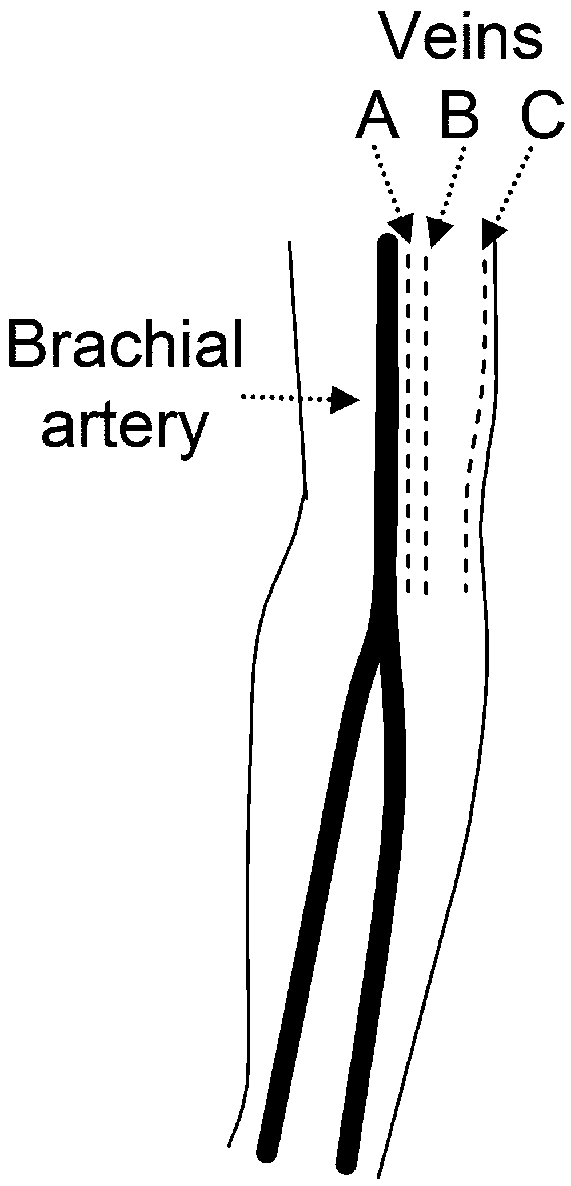
\includegraphics[width=0.4\textwidth]{627.png}
  \caption{Flujo sanguíneo de retorno en tres venas hipotéticas en el brazo derecho, etiquetadas como A, B y C.}
  \label{fig:627}
\end{figure}



\item[6.114] (problema avanzado) Determine el perfil de temperatura en una arteria ($T_{\text{a}}(x)$) y una vena ($T_{\text{v}}(x)$) que están lo suficientemente cerca como para formar un sistema de intercambio de calor a contracorriente \cite{69}, como en las Figs.~\ref{fig:618} y~\ref{fig:619}. Use el modelo de la Fig.~\ref{fig:628}. La arteria y la vena están tan próximas que existe una rápida transferencia de calor entre ellas. Por simplicidad, asuma que ambos vasos son idénticos y tienen un área de sección transversal $A$. La sangre fluye en ellos con una velocidad $v$ en las direcciones $x$ y $-x$, respectivamente, y tiene un calor específico $c$ y una densidad de masa $\rho$. (a) Explique por qué la conservación de la energía implica que la tasa de conducción de calor desde la arteria más caliente hacia la vena más fría (de la región I a la III en la Fig.~\ref{fig:628}) es igual a la pérdida de energía térmica en la convección de la sangre que fluye en la arteria (de la región I a la II, porque se enfría a lo largo de la dirección $x$), y que esto también es igual a la ganancia de energía térmica en la convección de la sangre que fluye en la vena (de la región IV a la III, porque se calienta a medida que viaja en la dirección $-x$). (b) Si la conductividad térmica es $K$, la distancia entre los vasos es $d$ (aproximadamente la suma de los espesores de los vasos) y el área de contacto es $w\,dx$, donde $w$ es el ancho del área de contacto a lo largo de la longitud $dx$, demuestre que la tasa de conducción de calor (por unidad de longitud) de la arteria a la vena es
\begin{equation}
R_{\text{conducción}} = \frac{K w}{d} (T_{\text{a}}(x) - T_{\text{v}}(x))
\label{eq:680}
\end{equation}
(c) Demuestre que la pérdida de flujo de calor por convección a lo largo de la arteria (por unidad de longitud) es
\begin{equation}
R_{\text{convección}} = -c \rho A v \frac{d T_{\text{a}}(x)}{dx}
\label{eq:681}
\end{equation}
(d) Combine (\ref{eq:680}) y (\ref{eq:681}) para obtener
\begin{equation}
\frac{d T_{\text{a}}(x)}{dx} = -\frac{K w}{c \rho A v d} (T_{\text{a}}(x) - T_{\text{v}}(x))
\label{eq:682}
\end{equation}
y de manera similar demuestre para las venas que
\begin{equation}
\frac{d T_{\text{v}}(x)}{dx} = -\frac{K w}{c \rho A v d} (T_{\text{a}}(x) - T_{\text{v}}(x))
\label{eq:683}
\end{equation}
(e) Resuelva estas dos ecuaciones para demostrar que la diferencia de temperatura entre la arteria y la vena es constante a lo largo de $x$ y que la temperatura en cada una disminuye linealmente con $x$, mediante
\begin{equation}
T_{\text{a}}(x) = T_{\text{a}}(0) - \frac{K w}{c \rho A v d} \Delta T x
\label{eq:684}
\end{equation}
y
\begin{equation}
T_{\text{v}}(x) = T_{\text{v}}(0) - \frac{K w}{c \rho A v d} \Delta T x,
\label{eq:685}
\end{equation}
donde $\Delta T = T_{\text{a}}(0) - T_{\text{v}}(0)$. (f) Dibuje $T_{\text{a}}(x)$ y $T_{\text{v}}(x)$ frente a $x$ a lo largo de una extremidad de longitud $L$, alternativamente si $(K w / c \rho A v d) L$ es $\ll 1$ o $\gg 1$. ¿Qué indican estas dos condiciones tan diferentes?

\begin{figure}[htbp]
  \centering
  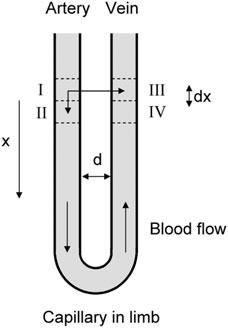
\includegraphics[width=0.45\textwidth]{628.png}
  \caption{Modelo de intercambio de calor a contracorriente entre una arteria y una vena. El calor de la arteria fluye ya sea desde la región I a la II por convección o desde la I a la III por conducción de calor (basado en \cite{69}).}
  \label{fig:628}
\end{figure}



\item[6.115] Alguien tiene una tasa metabólica diaria de $2200\text{ kcal}$, la cual se convierte completamente en calor. Si el $21\%$ de la pérdida de calor es a través de la evaporación de agua (en la piel y en los pulmones), ¿cuánta agua se evapora cada día (en L)?

\item[6.116] Derive (\ref{eq:670}).

\item[6.117] La ecuación (\ref{eq:670}) ignora explícitamente cualquier calentamiento o enfriamiento del vapor de agua. ¿Es esta una aproximación razonable? ¿Por qué?

\item[6.118] \label{prob:6118} Calcule los valores de los dos términos en (\ref{eq:670}) en unidades de $\text{kcal/día}$ asumiendo que la persona inspira aire a $20\ ^\circ\text{C}$ ($68\ ^\circ\text{F}$) que es muy seco ($0\%$ de humedad relativa) a una tasa de $6\text{ L/min}$ y expira aire (a la misma tasa, por supuesto) a $37\ ^\circ\text{C}$ ($98{,}6\ ^\circ\text{F}$) que está totalmente saturado con vapor de agua ($100\%$ de humedad relativa, $47{,}1\text{ mmHg}$ de presión parcial, $44{,}0\text{ g/m}^3$ de vapor de agua). ¿Qué tan significativa es cada pérdida para la pérdida de calor general del cuerpo?

\item[6.119] Repita el Problema~\ref{prob:6118} para los siguientes tres casos. (a) Para una persona que inhala aire a $20\ ^\circ\text{C}$ que está totalmente saturado con vapor de agua ($100\%$ de humedad relativa, $17{,}5\text{ mmHg}$ de presión parcial, $17{,}3\text{ g/m}^3$ de vapor de agua). (b) Para una persona que inhala aire a $40\ ^\circ\text{C}$ ($104\ ^\circ\text{F}$) que es muy seco ($0\%$ de humedad relativa). (c) Para una persona que inhala aire a $40\ ^\circ\text{C}$ que está totalmente saturado con vapor de agua ($100\%$ de humedad relativa, $55{,}3\text{ mmHg}$ de presión parcial, $51{,}1\text{ g/m}^3$ de vapor de agua). (d) Compare la tasa de enfriamiento general para estos tres casos entre sí y con la del Problema~\ref{prob:6118}.

\item[6.120] Explique cada uno de los factores que conducen al índice de calor.

\item[6.121] \label{prob:6121} El índice de calor, \text{HI}, se ha ajustado mediante
\begin{equation}
\begin{split}
\text{HI} = & -42{,}379 + 2{,}04901523 T + 10{,}14333127 R - 0{,}22475541 T R \\
& - 6{,}83783 \times 10^{-3} T^2 - 5{,}481717 \times 10^{-2} R^2 + 1{,}22874 \times 10^{-3} T^2 R \\
& + 8{,}5282 \times 10^{-4} T R^2 - 1{,}99 \times 10^{-6} T^2 R^2,
\end{split}
\label{eq:686}
\end{equation}
con el \text{HI} y la temperatura de bulbo seco ambiental $T$ en $^\circ\text{F}$ y la humedad relativa $R$ en $\%$ \cite{96,97}. (Esto asume una velocidad del viento de $5{,}65\text{ mph}$ ($5\text{ nudos}$) y tiene un error de $1{,}3\ ^\circ\text{F}$. La exposición a la luz solar directa puede aumentar el \text{HI} en hasta $15\ ^\circ\text{F}$). (a) Construya una tabla del índice de calor en $^\circ\text{F}$, con columnas que describan temperaturas secas (de bulbo) que van desde $80$ hasta $110\ ^\circ\text{F}$ (en pasos de $2\ ^\circ\text{F}$) y filas que describan la humedad relativa que va desde $40$ hasta $100\%$ (en pasos de $5\%$). (b) Marque las combinaciones de temperatura y humedad en la tabla para cada una de las cuatro regiones de advertencia de salud descritas en el texto.

\item[6.122] \label{prob:6122} Repita el Problema~\ref{prob:6121} para temperaturas de $27$ a $47\ ^\circ\text{C}$ (en pasos de $2\ ^\circ\text{C}$) y humedad relativa que va desde $40$ hasta $100\%$ (en pasos de $5\%$). (Convierta las temperaturas de $^\circ\text{C}$ a $^\circ\text{F}$ y luego use (\ref{eq:686})).

\item[6.123] (a) Convierta (\ref{eq:686}) de manera que tanto el \text{HI} como $T$ estén en $^\circ\text{C}$ en lugar de en $^\circ\text{F}$. (b) Repita el Problema~\ref{prob:6122}, trabajando directamente en $^\circ\text{C}$.

\item[6.124] Considere dos animales que modelaremos como cilindros \cite{69}. Ambos tienen temperaturas corporales de $35\ ^\circ\text{C}$ y viven en un entorno a $0\ ^\circ\text{C}$. El animal A tiene una longitud de $1\text{ m}$, un diámetro de $1\text{ m}$ y una capa de grasa de $1\text{ cm}$ de espesor (fuera del diámetro dado) para el aislamiento. El animal B tiene una longitud de $6\text{ m}$, un diámetro de $0{,}5\text{ m}$ y una capa de grasa de $4\text{ cm}$ de espesor para el aislamiento. (a) ¿Qué animal tiene más energía térmica (calor)? (b) ¿Qué animal pierde calor a una tasa más rápida? (Incluya las pérdidas alrededor del diámetro y en los extremos, y use una teoría simple, es decir, asuma un flujo plano e ignore las correcciones necesarias para el flujo cilíndrico). (c) ¿Qué animal pierde una fracción mayor de calor por unidad de tiempo? (d) ¿Qué animal espera que tenga la BMR más grande por unidad de masa? ¿Por qué? (e) ¿Son menores las pérdidas de calor para los animales con formas más esféricas, como el animal A, o para los animales con formas más de lápiz, como el animal B? (Ignore los diferentes espesores de las capas aislantes de grasa).

\item[6.125] \label{prob:6125} (a) Encuentre la temperatura de la piel asumiendo que $1\text{ cm}$ de grasa, la piel (sin propiedades de aislamiento térmico asumidas aquí) y $1\text{ cm}$ de ropa separan el núcleo corporal a $37\ ^\circ\text{C}$ y el exterior a $20\ ^\circ\text{C}$. Tome la conductividad térmica $K$ de la grasa como $5 \times 10^{-4}\text{ cal/cm-s-}^\circ\text{C}$ y la de la ropa como igual a la del aire, $6 \times 10^{-5}\text{ cal/cm-s-}^\circ\text{C}$ \cite{69}. (b) Encuentre la pérdida de calor por $\text{cm}^2$ por día. (c) Encuentre la pérdida de calor por día en todo el cuerpo utilizando un área de superficie de $1{,}5\text{ m}^2$. ¿Cómo se compara esto con la BMR? ¿Tiene sentido esto?

\item[6.126] Repita el Problema~\ref{prob:6125} asumiendo que la persona no lleva ropa.

\end{enumerate}

\section*{Referencias}

\begin{thebibliography}{106}
  \bibitem{1} T.C. Adam, E.S. Epel: Stress, eating and the reward system. \textit{Physiol. Behav.} 91, 449--458 (2007)
  \bibitem{2} B.K. Ahlborn: \textit{Zoological Physics: Quantitative Models, Body Design, Actions and Physical Limitations in Animals} (Springer, Berlín, 2004)
  \bibitem{3} L.C. Aiello, P. Wheeler: The expensive-tissue hypothesis: the brain and the digestive system in human and primate evolution. \textit{Curr. Anthropol.} 36, 199--221 (1995)
  \bibitem{4} R.M. Alexander: \textit{The Human Machine} (Columbia University Press, Nueva York, 1992)
  \bibitem{5} E. Archer, R.P. Shook, D.M. Thomas, T.S. Church, P.T. Katzmarzyk, J.R. Hébert, K.L. McIver, G.A. Hand, C.J. Lavie, S.N. Blair: 45-year trends in women's use of time and household management energy expenditure. \textit{PLoS One} 8, e56620 (2013)
  \bibitem{6} W.O. Atwater, F.G. Benedict: \textit{Experiments on the Metabolism of Matter and Energy in the Human Body}. Agricultural Bulletin No. 136 (U.S. Department of Agriculture, Washington, 1903)
  \bibitem{7} D.R. Bassett Jr., J. Pucher, R. Buehler, D.L. Thompson, S.E. Crouter: Walking, cycling, and obesity rates in Europe, North America, and Australia. \textit{J. Phys. Act. Health} 5, 795--814 (2008)
  \bibitem{8} G. Beccuti, S. Pannain: Sleep and obesity. \textit{Curr. Opin. Clin. Nutr. Metab. Care} 14, 402--412 (2011)
  \bibitem{9} G.B. Benedek, F.M.H. Villars: \textit{Physics with Illustrative Examples from Medicine and Biology}, 3 volúmenes, 2.ª ed. (AIP/Springer, Nueva York/Berlín, 2000)
  \bibitem{10} P.J. Berenson, W.G. Robertson: Temperature. En \textit{Bioastronautics Data Book}, editado por J.F. Parker Jr., V.R. West (NASA, Washington, 1973), Cap. 3, pp. 65--148
  \bibitem{11} K. Blaxter: \textit{Energy Metabolism in Animals and Man} (Cambridge University Press, Cambridge, 1989)
  \bibitem{12} S.N. Blair, H.W. Kohl, C.E. Barlow, R.S. Paffenbarger, L.W. Gibbons, C.A. Macera: Changes in physical fitness and all-cause mortality: a prospective study of healthy and unhealthy men. \textit{J. Am. Med. Assoc. (JAMA)} 273, 1093--1098 (1995)
  \bibitem{13} J.E. Blundell, N.A. King: Physical activity and regulation of food intake: current evidence. \textit{Med. Sci. Sports Exerc.} 31, S573--S589 (1999)
  \bibitem{14} S.M. Boback, C.L. Cox, B.D. Ott, R. Carmody, R.W. Wrangham, S.M. Secor: Cooking and grinding reduces the cost of meat digestion. \textit{Comp. Biochem. Physiol. A Mol. Integr. Physiol.} 148, 651--656 (2007)
  \bibitem{15} G. Boden, C. Homko, C.A. Barrero, T.P. Stein, X. Chen, P. Cheung, C. Fecchio, S. Koller, S. Merali: Excessive caloric intake acutely causes oxidative stress, GLUT4 carbonylation, and insulin resistance in healthy men. \textit{Sci. Transl. Med.} 7, 304re7 (2015)
  \bibitem{16} R.W. Bullard: Temperature regulation. En \textit{Physiology}, 4.ª ed., editado por E.E. Selkurt (Little Brown, Boston, 1976), p. 689
  \bibitem{17} N.F. Butte, J.K. Moon, W.W. Wong, J.M. Hopkinson, E.O.B. Smith: Energy requirements from infancy to adulthood. \textit{Am. J. Clin. Nutr.} 62(5), 1047S--1052S (1995)
  \bibitem{18} N.F. Butte, J.C. King: Energy requirements during pregnancy and lactation. \textit{Public Health Nutr.} 8, 1010--1027 (2005)
  \bibitem{19} J.R. Cameron, J.G. Skofronick, R. Grant: \textit{Physics of the Body}, 2.ª ed. (Medical Physics, Madison, 1999)
  \bibitem{20} N.A. Campbell, J.B. Reece: \textit{Biology}, 7.ª ed. (Pearson-Benjamin Cummings, San Francisco, 2005)
  \bibitem{21} R.N. Carmody, G.S. Weintraub, R.W. Wrangham: Energetic consequences of thermal and nonthermal food processing. \textit{Proc. Natl. Acad. Sci. (USA)} 108, 19199--19203 (2011)
  \bibitem{22} K. Cena, J.A. Clark: Thermal insulation of animal coats and human clothing. \textit{Phys. Med. Biol.} 23, 565--591 (1978)
  \bibitem{23} \textit{Composition of Foods: Raw, Processed, Prepared---USDA National Nutrient Database for Standard Reference, Release 26, Documentation and User Guide}, revisado en noviembre de 2013 (U.S. Department of Agriculture, 2013), \url{http://www.ars.usda.gov/sp2UserFiles/Place/12354500/Data/SR26/sr26_doc.pdf}
  \bibitem{24} J.L. Clapperton, J.P. Joyce, K.L. Blaxter: Estimates of the contribution of solar radiation to the thermal exchanges of sheep at a latitude of 55N. \textit{J. Agri. Sci. (Cambridge)} 64, 37--49 (1965)
  \bibitem{25} C.M. Cook, D.A. Schoeller: Physical activity and weight control: conflicting findings. \textit{Curr. Opin. Clin. Nutr. Metab. Care} 14, 419--424 (2011)
  \bibitem{26} K.E. Cooper, J.R. Kenyon: A comparison of temperatures measured in the rectum, esophagus, and on the surface of the aorta during hypothermia in man. \textit{Br. J. Surg.} 44, 616--619 (1957)
  \bibitem{27} P.S. Dodds, D.H. Rothman, J.S. Weitz: Re-examination of the 3/4-law of metabolism. \textit{J. Theor. Biol.} 209, 9--27 (2001)
  \bibitem{28} A.J. Donato, K. Tench, D.H. Glueck, D.R. Seals, I. Eskurza, H. Tanaka: Declines in physiological functional capacity with age: a longitudinal study in peak swimming performance. \textit{J. Appl. Physiol.} 94, 764--769 (2003)
  \bibitem{29} H.M. Dunsworth, A.G. Warrener, T. Deacon, P.T. Ellison, H. Pontzer: Metabolic hypothesis for human altriciality. \textit{Proc. Natl. Acad. Sci. USA} 109, 15212--15216 (2012)
  \bibitem{30} P.T. Ellison: \textit{On Fertile Ground: A Natural History of Human Reproduction} (Harvard University Press, Cambridge, 2003)
  \bibitem{31} P. Evenepoel, B. Geypens, A. Luypaerts, M. Hiele, Y. Ghoos, P. Rutgeerts: Digestibility of cooked and raw egg protein in humans as assessed by stable isotope techniques. \textit{J. Nutr.} 128, 1716--1722 (1998)
  \bibitem{32} P. Evenepoel, D. Claus, B. Geypens, M. Hiele, K. Geboes, P. Rutgeerts, Y. Ghoos: Amount and fate of egg protein escaping assimilation in the small intestine of humans. \textit{Am. J. Physiol. Cell Physiol.} 277, G935--G943 (1999)
  \bibitem{33} FAO/WHO/UNU: \textit{Energy and Protein Requirements. Report of a Joint Experts Consultation}. WHO Technical Report Series No. 724 (Organización Mundial de la Salud, Ginebra, 1985), \url{http://www.fao.org/docrep/003/aa040e/aa040e00.htm}
  \bibitem{34} R. Floud, R.W. Fogel, B. Harris, S.C. Hong: \textit{The Changing Body: Health, Nutrition, and Human Development in the Western World Since 1700} (Cambridge University Press, Cambridge, 2011)
  \bibitem{35} M.L. Foss, S.J. Keteyian: \textit{Fox's Physiological Basis for Exercise and Sport}, 6.ª ed. (McGraw-Hill, Boston, 1998)
  \bibitem{36} E.L. Fox, D.K. Matthews: \textit{Interval Training Conditioning for Sport and General Fitness} (Saunders, Filadelfia, 1974)
  \bibitem{37} S.M. Frank, Y. Shir, S.N. Raja, L.A. Fleisher, C. Beattie: Core hypothermia and skin-surface temperature gradients. Epidural versus general anesthesia and the effects of age. \textit{Anesthesiology} 80, 502--508 (1994)
  \bibitem{38} R.A. Freitas Jr.: \textit{Nanomedicine, Volume I: Basic Capabilities} (Landes Bioscience, Austin, 1999)
  \bibitem{39} J.S. Garrow: Resting metabolic rate as a determinant of energy expenditure in man. En \textit{Substrate and Energy Metabolism in Man}, editado por J.S. Garrow, D. Halliday (Libbey, Londres, 1985), pp. 102--107
  \bibitem{40} R.C. Garry, R. Passmore, G.M. Warnock, J.V.G.A. Durnin: Expenditure of energy and the consumption of food by miners and clerks, Fife, Scotland. Medical Research Council Special Report Series 289 (HMSO, Londres, 1955)
  \bibitem{41} S.E. Gebhardt, R.G. Thomas: \textit{Nutritive Value of Foods}, U.S. Department of Agriculture, Agricultural Research Service, Home and Garden Bulletin 72 (2002)
  \bibitem{42} J.F. Gillooly, J.H. Brown, G.B. West, V.M. Savage, E.L. Charnov: Effects of size and temperature on metabolic rates. \textit{Science} 293, 2248--2251 (2001)
  \bibitem{43} C.V. Gisolfi, C.B. Wenger: Temperature regulation during exercise: old concepts, new ideas. \textit{Exerc. Sport Sci. Rev.} 12, 339--372 (1984)
  \bibitem{44} H. Gray: The Organs of the Senses and the Common Integument. En \textit{Anatomy of the Human Body}, 20.ª ed. (Lea \& Febiger, Filadelfia, 1918)
  \bibitem{45} A.C. Guyton, J.E. Hall: \textit{Human Physiology and Mechanisms of Disease}, 6.ª ed. (Saunders, Filadelfia, 1997)
  \bibitem{46} K.A. Hammond, J. Diamond: Maximal sustained energy budgets in humans and animals. \textit{Nature} 386, 457--462 (1997)
  \bibitem{47} W.P.T. James, E.C. Schofield: \textit{Human Energy Requirements: A Manual for Planners and Nutritionists} (Oxford University Press, Oxford, 1990)
  \bibitem{48} D.J. Johns, J. Hartmann-Boyce, S.A. Jebb, P. Aveyard: Diet or exercise interventions vs combined behavioral weight management programs: A Systematic review and meta-analysis of direct comparisons. \textit{J. Acad. Nutr. Diet.} 114, 1557--1568 (2014)
  \bibitem{49} W.V. Judy: Body temperature regulation. En \textit{Physiology}, 5.ª ed., Cap. 28, editado por E.E. Selkurt (Little Brown, Boston, 1984)
  \bibitem{50} M.C.K. Khoo: \textit{Physiological Control Systems: Analysis, Simulation, and Estimation} (IEEE, Piscataway, 2000)
  \bibitem{51} M. Kleiber: Body size and metabolism. \textit{Hilgardia} 6, 315--353 (1932)
  \bibitem{52} M. Kleiber: Body size and metabolic rate. \textit{Physiol. Rev.} 27, 511--541 (1947)
  \bibitem{53} M. Kleiber: \textit{The Fire of Life: An Introduction to Animal Energetics} (Wiley, Nueva York, 1961)
  \bibitem{54} T.M. Larsen, S.M. Dalskov, M. van Baak, S.A. Jebb, A. Papadaki, A.F. Pfeiffer, J.A. Martinez, T. Handjieva-Darlenska, M. Kunesová, M. Pihlsgård, S. Stender, C. Holst, W.H. Saris, A. Astrup: Diets with high or low protein content and glycemic index for weight-loss maintenance. \textit{N. Engl. J. Med.} 363, 2102--2113 (2010)
  \bibitem{55} A.L. Lehninger: \textit{Biochemistry: The Molecular Basis of Cell Structure and Function}, 2.ª ed. (Worth, Nueva York, 1975)
  \bibitem{56} D.E. Lieberman: \textit{The Story of the Human Body: Evolution, Health, and Disease} (Pantheon, Nueva York, 2013)
  \bibitem{57} H. Lodish, A. Berk, P. Matsudaira, C.A. Kaiser, M. Krieger, M.P. Scott, S.L. Zipursky, J. Darnell: \textit{Molecular Cell Biology}, 5.ª ed. (Freeman, Nueva York, 2004)
  \bibitem{58} M. Lof, H. Olausson, K. Bostrom, B. Janerot-Sjöberg, A. Sohlstrom, E. Forsum: Changes in basal metabolic rate during pregnancy in relation to changes in body weight and composition, cardiac output, insulin-like growth factor I, and thyroid hormones and in relation to fetal growth. \textit{Am. J. Clin. Nutr.} 81, 678--685 (2005)
  \bibitem{59} D.L. Longo, A.S. Fauci, D.L. Kasper, S.L. Hauser, J. Jameson, J. Loscalzo (eds.): \textit{Harrison's Principles of Internal Medicine}, 18.ª ed. (McGraw-Hill, Nueva York, 2011)
  \bibitem{60} R. Margaria, P. Cerretelli, P. Aghemo, G. Sassi: Energy cost of running. \textit{J. Appl. Physiol.} 18, 367--370 (1963)
  \bibitem{61} R.R. Markwald, E.L. Melanson, M.R. Smith, J. Higgins, L. Perreault, R.H. Eckel, K.P. Wright Jr.: Impact of insufficient sleep on total daily energy expenditure, food intake, and weight gain. \textit{Proc. Natl. Acad. Sci. (USA)} 110, 5695--5700 (2013)
  \bibitem{62} F.W. Marlowe: Hunter-gatherers and human evolution. \textit{Evol. Anthropol.} 14, 54--67 (2005)
  \bibitem{63} A.G. Marshall: \textit{Biophysical Chemistry} (Wiley, Nueva York, 1978)
  \bibitem{64} R.D. Mattes, P.M. Kris-Etherton, G.D. Foster: Impact of peanuts and tree nuts on body weight and healthy weight loss in adults. \textit{J. Nutr.} 138, 1741S--1745S (2008)
  \bibitem{65} T.A. McMahon: Size and shape in biology. \textit{Science} 179, 1201--1204 (1973)
  \bibitem{66} T.A. McMahon: \textit{Muscles, Reflexes, and Locomotion} (Princeton University Press, Princeton, 1984)
  \bibitem{67} A. McTiernan, B. Sorensen, M.L. Irwin, A. Morgan, Y. Yasui, R.E. Rudolph, C. Surawicz, J.W. Lampe, P.D. Lampe, K. Ayub, J.D. Potter: Exercise effect on weight and body fat in men and women. \textit{Obesity} 15, 1496--1512 (2007)
  \bibitem{68} A.L. Merrill, B.K. Watt: \textit{Energy Value of Foods---Basis and Derivation}. Agriculture Handbook No. 74, revisado en febrero de 1973 (U.S. Department of Agriculture, 1973), \url{http://www.ars.usda.gov/SP2UserFiles/Place/12354500/Data/Classics/ah74.pdf}
  \bibitem{69} H.J. Metcalf: \textit{Topics in Classical Biophysics} (Prentice-Hall, Englewood Cliffs, 1980)
  \bibitem{70} J.L. Monteith: \textit{Principles of Environmental Physics} (Edward Arnold, Londres, 1973)
  \bibitem{71} L.E. Mount: \textit{Adaptation to the Thermal Environment} (Edward Arnold, Londres, 1979)
  \bibitem{72} L.E. Mount: En \textit{Heat Loss from Animals and Man}, editado por J.L. Monteith, L.E. Mount (Butterworths, Londres, 1974)
  \bibitem{73} J.M. Moya, L. Phillips, J. Sanford, M. Wooton, A. Gregg, L. Schuda: A review of physiological and behavioral changes during pregnancy and lactation: potential exposure factors and data gaps. \textit{J. Expo. Sci. Environ. Epidemiol.} 24, 449--458 (2014)
  \bibitem{74} M.W. Moyer: Supercharging brown fat to battle obesity: why turning down the thermostat could help win the battle of the bulge. \textit{Scientific American} 311(2) (2014), \url{http://www.scientificamerican.com/article/supercharging-brown-fat-to-battle-obesity/}
  \bibitem{75} D.L. Nelson, M.M. Cox: \textit{Lehninger Principles of Biochemistry}, 4.ª ed. (Worth, Nueva York, 2005)
  \bibitem{76} J.A. Novotny, S.K. Gebauer, D.J. Baer: Discrepancy between Atwater factor predicted and empirically measured energy value of almonds in human diets. \textit{Am. J. Clin. Nutr.} 96, 296--301 (2012)
  \bibitem{77} R. Passmore, J.V.G.A. Durnin: \textit{Energy, Work and Leisure} (Heinemann Educational Books, Londres, 1967)
  \bibitem{78} C.C. Peterson, K.A. Nagy, J. Diamond: Sustained metabolic scope. \textit{Proc. Natl. Acad. Sci. USA} 87, 2324--2328 (1990)
  \bibitem{79} A. Pietrobelli, D.B. Allison, S. Heshka, M. Heo, Z.M. Wang, A. Bertkau, B. Laferrère, M. Rosenbaum, J.F. Aloia, F.X. Pi-Sunyer, S.B. Heymsfield: Sexual dimorphism in the energy content of weight change. \textit{Int. J. Obes.} 26, 1339--1348 (2002)
  \bibitem{80} M.H. Pimentel, D. Pimentel (eds.): \textit{Food, Energy, and Society}, 3.ª ed. (CRC Press, Boca Raton, 2007)
  \bibitem{81} P. Poirier, J.-P. Després: Exercise in weight management of obesity. \textit{J. Cardiol. Clin.} 19, 459--470 (2001)
  \bibitem{82} H. Pontzer, D.A. Raichlen, B.M. Wood, A.Z.P. Mabulla, S.B. Racette, F.W. Marlowe: Hunter-Gatherer Energetics and Human Obesity. \textit{PLoS One} 7(7), doi:10.1371/journal.pone.0040503 (2012)
  \bibitem{83} P.E. di Prampero: The energy cost of human locomotion on land and in water. \textit{Int. J. Sports Med.} 7, 55--72 (1986)
  \bibitem{84} A.M. Prentice, R.G. Whitehead, S.B. Roberts, A.A. Paul: Long-term energy balance in child-bearing Gambian women. \textit{Am. J. Clin. Nutr.} 34, 2790--2799 (1981)
  \bibitem{85} A.M. Prentice, C.J. Spaaij, G.R. Goldberg, S.D. Poppitt, J.M. van Raaij, M. Totton, D. Swann, A.E. Black: Energy requirements of pregnant and lactating women. \textit{Eur. J. Clin. Nutr.} 50 (Supl. 1), S82--S110 (1996)
  \bibitem{86} L.G.C.E. Pugh: The influence of wind resistance in running and walking and the efficiency of work against horizontal and vertical forces. \textit{J. Physiol. (London)} 48, 518--522 (1971)
  \bibitem{87} C. Reiff, K. Marlatt, D.R. Dengel: Difference in caloric expenditure in sitting versus standing desks. \textit{J. Phys. Act. Health} 9, 1009--1011 (2012)
  \bibitem{88} V.C. Rideout: \textit{Mathematical and Computer Modeling of Physiological Systems} (Prentice-Hall, Englewood Cliffs, 1991)
  \bibitem{89} R.M. Ross, A.S. Jackson: \textit{Exercise Concepts, Calculations, and Computer Applications} (Benchmark, Carmel, 1990)
  \bibitem{90} W.N. Schofield: Predicting basal metabolic rate, new standards and review of previous work. \textit{Hum. Nutr. Clin. Nutr.} 39C (Supl. 1), 5--41 (1985)
  \bibitem{91} G.G. Schwartz, L.A. Rosenblum: Allometry of primate hair density and the evolution of human hairlessness. \textit{Am. J. Phys. Anthropol.} 55, 9--12 (1981)
  \bibitem{92} J.W. Severinghaus: Temperature gradients during hypothermia. \textit{Ann. New York Acad. Sci.} 80, 515--521 (1959)
  \bibitem{93} J. Singh, A.M. Diaz, E. Prentice, W.A. Coward, J. Ashford, M. Sawyer, R.G. Whitehead: Energy expenditure of Gambian women during peak agricultural activity measured by the doubly-labelled water method. \textit{Brit. J. Nutr.} 62, 315--329 (1989)
  \bibitem{94} D.W. Spady, P.R. Payne, D. Picou, J.C. Waterlow: Energy balance during recovery from malnutrition. \textit{Am. J. Clin. Nutr.} 29, 1073--1088 (1976)
  \bibitem{95} A. Stalheim-Smith, G.K. Fitch: \textit{Understanding Human Anatomy and Physiology} (West, St. Paul, MN, 1993)
  \bibitem{96} R.G. Steadman: The assessment of sultriness. Part I. A temperature-humidity index based on human physiology and clothing science. \textit{J. Appl. Meteorol.} 18, 861--873 (1979)
  \bibitem{97} R.B. Stull: \textit{Meteorology for Scientists and Engineers}, 2.ª ed. (Brooks Cole, Pacific Grove, 1999)
  \bibitem{98} W.C. Swinbank: Long wave radiation from clear skies. \textit{Q. J. R. Meteorol. Soc.} 89, 339--351 (1963)
  \bibitem{99} H.T. Tanaka, D.R. Seals: Topical review: endurance exercise performance in Masters athletes: age-associated changes and underlying physiological mechanisms. \textit{J. Physiol.} 586, 55--63 (2008)
  \bibitem{100} \textit{USDA National Nutrient Database for Standard Reference, Release 26}. Nutrient Data Laboratory (U.S. Department of Agriculture, Agricultural Research Service, 2013), \url{http://www.ars.usda.gov/ba/bhnrc/ndl}
  \bibitem{101} A.A. van der Klaauw, I.S. Farooqi: Review: the hunger genes: pathways to obesity. \textit{Cell} 161, 119--132 (2015)
  \bibitem{102} D.T. Villareal, S. Chode, N. Parimi, D.R. Sinacore, T. Hilton, R. Armamento-Villareal, N. Napoli, C. Qualls, K. Shah: Weight loss, exercise, or both and physical function in obese older adults. \textit{N. Engl. J. Med.} 364, 1218--1229 (2011)
  \bibitem{103} H.T. Waaler: Height, weight and mortality. The Norwegian experience. \textit{Acta Medica Scand.} 215 (Supl. 679), 1--56 (1984)
  \bibitem{104} P.E. Wheeler: The thermoregulatory advantages of hominid bipedalism in open equatorial environments: The contribution of increased convective heat loss and cutaneous evaporative cooling. \textit{J. Hum. Evol.} 21, 107--115 (1991)
  \bibitem{105} D.R. Wilkie: Man as a source of mechanical power. \textit{Ergonomics} 3, 1--8 (1960)
  \bibitem{106} J.H. Wilmore, D.L. Costill: \textit{Physiology of Sport and Exercise}, 3.ª ed. (Human Kinetics, Champaign, 2004)
  \bibitem{107} D.A. Winter: \textit{Biomechanics and Motor Control of Human Movement}, 3.ª ed. (Wiley, Nueva York, 2005)
  \bibitem{108} M. Wishnofsky: Caloric equivalents of gained or lost weight. \textit{Am. J. Clin. Nutr.} 6, 542--546 (1958)
\end{thebibliography}

% Control de Calidad: 13 párrafos de problemas + 108 referencias origen -> 13 párrafos de problemas + 108 referencias salida. Mapeo 1:1 verificado. Sin omisiones.

\end{document}

